% \iffalse meta-comment
%<*internal>
\iffalse
%</internal>
%<*readme>
----------------------------------------------------------------
phd-pkgmanager --- a package to shorten preambles
E-mail: yannislaz@gmail.com
Released under the LaTeX Project Public License v1.3c or later
See http://www.latex-project.org/lppl.txt
----------------------------------------------------------------
This file provides a phd for defining a class.
%</readme>
%<*readmemd>
###The `phd` LaTeX2e package

The `phd` latex package and the class with the same name provide
convenient methods to create new styles for books, reports
and articles. It also loads the most commonly used packages 
and resolves conflicts.

This work consists of the file  `phd.dtx`,
and the derived files   `phd.ins`,  `phd.pdf`, and `phd.sty`.

###Installation

run
          phd-lua.bat on windows
           pdflatex phd.dtx
           makeindex -s gind.ist -g phd 

If you have any difficulties with the package come and join us at
http://tex.stackexchange.com and post a new question or
add a comment at http://tex.stackexchange.com/a/45023/963.
or send me a message at  yannislaz at gmail.com

### Documentation

The package was written using the `doc` and `docscript` packages,
so that it is self documented in a literary programming style. 
The .pdf is a fat document, providing over fifty book styles (the
equivalent of classes) plus there is a lot of write-up on the inner
workings of TeX and LaTeX2e. However, you don't need to know much
to use it.

      \usepackage{phd}
      %%%%%%%%%%%%%%%%%%%%%%%%%%%%%%%%%%%%%%%%%%%
%%%%%%  STYLE 13
%%%%%%%%%%%%%%%%%%%%%%%%%%%%%%%%%%%%%%%%%%%

\cxset{style13/.style={
 name={Chapter},
 numbering=arabic,
 number font-size=\HUGE,
 number font-family=\sffamily,
 number font-weight=\bfseries,
 number color=\color{gray!50},
 number before=\par\vspace*{5pt}\hfill\hfill,
 number dot=,
 number after={\hspace*{7pt}\par},
 number position=rightname,
 chapter font-family=\sffamily,
 chapter font-weight=\normalfont,
 chapter font-size=\LARGE,
 chapter before={\thickrule\vspace*{20pt}\par\hfill\hfill},
 chapter after={\vskip0pt\par},
 chapter color={black!50},
 title beforeskip={\vspace*{10pt}},
 title afterskip={\vspace*{50pt}\par},
 title before={\hfill\hfill\raggedleft},
 title after={},
 title font-family=\sffamily,
 title font-color=\color{thered},
 title font-weight=\bfseries,
 title font-size=\huge,
 section indent=-1em,
 section align=\raggedright,
 section numbering=arabic,
 section indent=0pt,
 section beforeskip=0pt,
 section afterskip=\baselineskip,
 subsection align=\raggedright,
 subsection font-family=\sffamily,
 subsection font-weight=\bfseries,
 subsection font-size=\large,
 subsection font-shape=\itshape,
 subparagraph number after=\space,
}
}

\def\setstyle#1{\cxset{style#1}%
 \renewsection\renewsubsection\renewsubsubsection%
 \renewparagraph\renewsubparagraph}

\setstyle{13}


\chapter{Introduction to Chapter\\ Style Thirteen}

\section{A Brief History of Biomedical\\ Fluid Mechanics}
\lorem
\medskip
\begin{figure}[ht]
\centering
\includegraphics[width=0.45\textwidth]{./chapters/chapter14}
\includegraphics[width=0.45\textwidth]{./chapters/chapter14a}
\end{figure}
\lorem


All choices, are made via an extended key-value interface. 
Although not a compliment, it resembles CSS and the keys are a bit verbose but
attributes are easy to change and have a consistent and easy to remember interface.

To set or add a key we only use one command:

      \cxset{chapter name font-size = Huge,
             chapter number font-size = HUGE} 

### Future Development

This is still an experimental version, but I will retain the
interface in future releases. There is a large amount of
work still to be carried out to improve the template styles
provided, to test it more thoroughly and to add a number of
improvements in the special designs. At present I estimate
that I have completed about 70% of the work that needs
to be done.

__The package as it stands is not production stable.__ 


%</readmemd>
%
%<*TODO>
1. On final round add pkg options. This was left as last in order not to solve problems by adding
    options. Too many options are not a good User Interface.
2.  Finish symbol management, both text and math. Math already 60% incorporated.
3.  Better integration of indexing commands.   
4.  Revisit layout manager for Chapters. Broke again in tests.
5.  Docs. Add all references.
6.  Incorporate phd class for more flexibility.
7. Improve package manager.
8. Group script loading for better font management.
9. General font management to relook it again.
10. Add all style sections (about 100 already prepared). Once they
     are all working issue beta version.
%</TODO>
%<*internal>
\fi
\def \nameofplainTeX{plain}
\ifx\fmtname\nameofplainTeX\else
  \expandafter\begingroup
\fi
%</internal>
%<*install>
\input docstrip.tex
\keepsilent
\askforoverwritefalse
\preamble
----------------------------------------------------------------
phd --- A package to beautify documents.
E-mail: yannislaz@gmail.com
Released under the LaTeX Project Public License v1.3c or later
See http://www.latex-project.org/lppl.txt
----------------------------------------------------------------
\endpreamble

%\BaseDirectory{C:/users/admin/my documents/github/phd}
%\usedir{MWE}
\generate{\file{\jobname.sty}{
  \from{\jobname.dtx}{DOCUM}
   }
  }

%\nopreamble\nopostamble

%</install>

%<install>\endbatchfile
%<*internal>
%\usedir{tex/latex/phd}
\generate{
  \file{\jobname.ins}{\from{\jobname.dtx}{install}}
}
\nopreamble\nopostamble

\generate{
	\file{README.txt}{\from{\jobname.dtx}{readme}}
  }

\generate{
  \file{README.md}{\from{\jobname.dtx}{readmemd}}
}
\generate{
  \file{TODO.tex}{\from{\jobname.dtx}{TODO}}
}

\ifx\fmtname\nameofplainTeX
  \expandafter\endbatchfile
\else
  \expandafter\endgroup
\fi
%</internal>
%<*driver>

%\listfiles
%gdef\@onlypreamble{} % TO BE REMOVED NEEDED FOR TUTS
\documentclass[oneside,11pt,a4paper]{ltxdoc}
\usepackage[bottom=2cm]{geometry}
\savegeometry{std}
% \usepackage[style=mla]{biblatex}
\usepackage[unicodemath=on]{phd}
\usepackage{phd-lowersections}
\usepackage{phd-runningheads}
\usepackage{phd-documentation}
\pagestyle{headings}
\sethyperref

\begin{filecontents}{defaults-chapters}
%%    General Defaults for Chapters
\cxset{%    
    chapter title margin-top-width    =  0cm,
    chapter title margin-right-width  =  1cm,
    chapter title margin-bottom-width = 10pt,
    chapter title margin-left-width   = 0pt,
    chapter align                     = left,
    chapter title align               = left, %checked
    chapter name                      = hang,
    chapter format                    = hdr,
    chapter font-size                 = Huge,
    chapter font-weight               = bold,
    chapter font-family               = sffamily,
    chapter font-shape                = upshape,
    chapter color                     = black,
    chapter number prefix             = ,
    chapter number suffix             = ,
    chapter numbering                 = arabic,
    chapter indent                    = 0pt,
    chapter beforeskip                = -3cm,
    chapter afterskip                 = 30pt,
    chapter afterindent               = off,
    chapter number after              = ,
    chapter arc                       = 0mm,
    chapter background-color          = bgsexy,
    chapter afterindent               = off,
    chapter grow left                 = 0mm,
    chapter grow right                = 0mm, 
    chapter rounded corners           = northeast,
    chapter shadow                    = fuzzy halo,
    chapter border-left-width         = 0pt,
    chapter border-right-width     = 0pt,
    chapter border-top-width       = 0pt,
    chapter border-bottom-width    = 0pt,
    chapter padding-left-width     = 0pt,
    chapter padding-right-width    = 10pt,
    chapter padding-top-width      = 10pt,
    chapter padding-bottom-width   = 10pt,
    chapter number color           = white,
    chapter label color            = white,    
    }
 \cxset{    
    chapter number font-size        = huge,
    chapter number font-weight      = bfseries,
    chapter number font-family      = sffamily,
    chapter number font-shape       = upshape,
    chapter number align            = Centering,
    }
\cxset{%    
     chapter title font-size        = Huge,
     chapter title font-weight      = bold,
     chapter title font-family      = calligra,
     chapter title font-shape       = upshape,
     chapter title color            = black,
     }    
\end{filecontents}
%% LaTeX2e file `defaults-chapters'
%% generated by the `filecontents' environment
%% from source `phd-lowersections' on 2015/07/21.
%%
%%    General Defaults for Chapters
\cxset{%
    chapter title margin-top-width    =  0cm,
    chapter title margin-right-width  =  1cm,
    chapter title margin-bottom-width = 10pt,
    chapter title margin-left-width   = 0pt,
    chapter align                     = RaggedLeft,
    chapter title align               = Centering, %checked
    chapter name                      = Chapter,
    chapter format                    = block,
    chapter font-size                 = HHUGE,
    chapter font-weight               = bold,
    chapter font-family               = sffamily,
    chapter font-shape                = upshape,
    chapter color                     = black,
    chapter number prefix             = ,
    chapter number suffix             = ,
    chapter numbering                 = arabic,
    chapter indent                    = 0pt,
    chapter beforeskip                = -1sp,
    chapter afterskip                 = 30pt,
    chapter afterindent               = off,
    chapter number after              = ,
    chapter arc                       = 0mm,
    chapter background-color       = bgsexy,
    chapter afterindent            = off,
    chapter grow left              = 0mm,
    chapter grow right             = 0mm,
    chapter rounded corners        = northeast,
    chapter shadow                 = fuzzy halo,
    chapter border-left-width      = 0pt,
    chapter border-right-width     = 0pt,
    chapter border-top-width       = 0pt,
    chapter border-bottom-width    = 0pt,
    chapter padding-left-width     = 0pt,
    chapter padding-right-width    = 10pt,
    chapter padding-top-width      = 10pt,
    chapter padding-bottom-width   = 10pt,
    chapter number color           = white,
    chapter label color            = white,
    }
 \cxset{
    chapter number font-size        = huge,
    chapter number font-weight      = bfseries,
    chapter number font-family      = sffamily,
    chapter number font-shape       = upshape,
    chapter number align            = Centering,
    }
\cxset{%
     chapter title font-size        = HHUGE,
     chapter title font-weight      = bold,
     chapter title font-family      = sffamily,
     chapter title font-shape       = upshape,
     chapter title color            = white,
     }
  


\definecolor{creamy}{HTML}{FDEBD7}
\cxset{chapter title color= creamy,
       chapter label color = creamy,
       chapter number color = creamy,
       chapter number font-size = Huge,
       subsection title color = creamy,
       chapter name = CHAPTER,
       chapter label case = upper,
       chapter number align=left,
       part format = traditional,
       part background-color=spot,
       part beforeskip                = -3cm,
       part afterskip                 = 30pt,
       }
\usepackage{makeidx}       
\makeindex
\begin{document}
\parindent1em
\coverpage{monkey}{Book Design Monographs}{Camel Press}{INDEXING}{AND DOCUMENTATION} 
\pagestyle{empty}
%\coverpage{habtoor-city}{Delay Claim}{HLS-DSE/JV}{HABTOOR CITY}{MEP CLAIM} 
\secondpage
\pagestyle{empty}
\clearpage
\ExplSyntaxOn
\tableofcontents
\ExplSyntaxOff
\pagestyle{empty}
\setcounter{secnumdepth}{6}
\parskip0pt plus.1ex minus.1ex
\mainmatter
\pagenumbering{arabic}
\pagestyle{headings}        
%       
%\def\storyi{The best graphics package ever developed is the TikZ package. 
Its parent package is PGF which is short of a miracle that has been programmed
using \tex, a more than thirty years old program. This has taken over almost all other
packages and is very popular with newcomers to \latex. It is frustrating at first, but once 
you over the basic ideas and concepts it opens infinite possibilities for typesetting
great articles and books.}



\cxset{chapter format=stewart,
       texti=\storyi,
       textii=\storyi}

\newcommand\seepgfmanual[1]{%
    \textit{see} the PGFmanual page #1}%
    
%\cxset{chapter format = traditional}    
\chapter{TikZ}

\section{The \protect\texttt{TikZ} package}
\pkg{TikZ}, a high-level interface to \pkg{PGF}, is a language-based tool for specifying graphics.
It uses familiar graphics-related concepts, such as point, line, and circle and
has a concise and natural syntax. It meshes well with pdfLATEX in the sense that
no additional processing steps are needed. Another positive aspect of \pkg{TikZ} is
its ability to blend \tex fonts, symbols, and mathematics within the generated
graphics.


All the TikZ commands can be used inline using \docAuxCommand{tikz} or within the \docAuxCommand{tikzpicture} environment. When we want to use captions and labels, we enclose it in the figure environment or use \docAuxCommand{captionof}, but it can be called anywhere in the text or math of a Tex document:

\begin{teXXX}
\begin{figure}
\centering
%\tikzset{external/force remake}
\begin{tikzpicture}
... TikZ commands ...
\end{tikzpicture}
\caption{A diagram drawn with TikZ.}
\label{Fig:_diagram1}
\end{figure}
\end{teXXX}

We can also use them in math:

\begin{teXXX}
\begin{align*}
\int dx\; f(x) =
\alpha
%\tikzset{external/force remake}
\begin{tikzpicture}
... TikZ commands ...
\end{tikzpicture}
\end{align*}
\end{teXXX}



\section{Draw simple lines}

\begin{texexample}{Draw a Line}{ex:line}
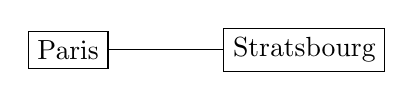
\begin{tikzpicture}
\node[draw] (S1) at (0,0) {Paris};
\node[draw] (S2) at (3,0) {Stratsbourg};
\draw (S1) -- (S2);
\end{tikzpicture}
\end{texexample}


The syntax of the command is:

|\node|\oarg{options} (\meta{name}) at (\meta{position}) |{|\meta{contents}|}|

If we look
 carefully, we see that the two writings give
Slightly different results:
- In the first case, node is an operation executed on a path. We
Can consider each node as a decoration of the point at which it
is associated. The line drawn by the draw command joins two points, the
Nodes are objects added later and centered on points. The option
Draw of the node trace operation the node outline.
- In the second case, \ node is a TikZ command which allows to define
A node, to name it and to draw it. One can then consider the
Nodes as pre-existing objects that will then be linked with the \docAuxCommand{node}.


\begin{texexample}{Draw a Line}{ex:line}
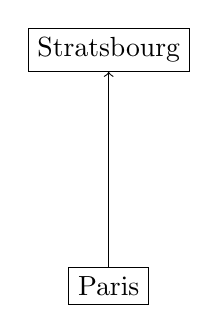
\begin{tikzpicture}
\node[draw] (S1) at (0,0) {Paris};
\node[draw] (S2) at (0,3) {Stratsbourg};
\draw[->] (S1) -- (S2);
\end{tikzpicture}
\end{texexample}

The basic building block of all pictures in \tikzname is the path. A path is a series of straight lines and curves
that are connected (that is not the whole picture, but let us ignore the complications for the moment). You
start a path by specifying the coordinates of the start position as a point in round brackets, as in (0,0).
This is followed by a series of \enquote{path extension operations.}


\begin{texexample}{Draw a Line}{ex:line}
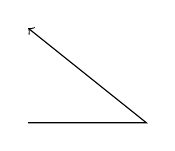
\begin{tikzpicture}
\draw[->] (0,0) -- (1.5,0) -- (0, 1.2);
\end{tikzpicture}
\end{texexample}


\subsection*{Adding Text} 

So far we have seen how to draw lines and arcs. However, an important component is still missing the addition of text. When
\tikzname is constructing a path and it encounters the keyword |node| typically followed by some options  it reads a \textit{node specification}. Options can typically follow and then it terminates by curly brackets. 
 

\begin{texexample}{Draw a Line}{ex:line}
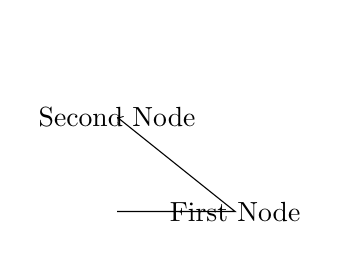
\begin{tikzpicture}
\draw[->] (0,0) -- (1.5,0) node {First Node} -- (0, 1.2) node[shape = circle] {Second Node};
\end{tikzpicture}
\end{texexample}


The \docAuxCommand*{node} can be used to abbreviate the operation. A longer example can demonstrate this better. How can we draw the following figure?

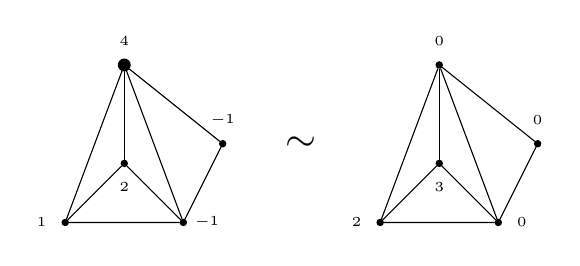
\begin{tikzpicture}
\node[circle,fill=black,inner sep=0.8pt,draw] (a) at (0,0) {};
\node[circle,fill=black,inner sep=0.8pt,draw] (b) at (1.5,0) {};
\node[circle,fill=black,inner sep=1.5pt,draw] (c) at (.75,2) {};
\node[circle,fill=black,inner sep=0.8pt,draw] (d) at (0.75,.75) {};
\node[circle,fill=black,inner sep=0.8pt,draw] (e) at (2,1) {};


\node () at (-0.3,0) {\tiny$1$};
\node () at (0.75,0.45) {\tiny$2$};
\node () at (0.75,2.3) {\tiny$4$};
\node () at (2,1.3) {\tiny$-1$};
\node () at (1.8,0) {\tiny$-1$};

\draw (a)--(b)--(e)--(c) --(a)--(d)--(b)--(c);
\draw (c)--(d);

\node at (3,1) {\Large{$\sim$}};

\begin{scope}[shift={(+4,0)}]
\node[circle,fill=black,inner sep=0.8pt,draw] (a) at (0,0) {};
\node[circle,fill=black,inner sep=0.8pt,draw] (b) at (1.5,0) {};
\node[circle,fill=black,inner sep=0.8pt,draw] (c) at (.75,2) {};
\node[circle,fill=black,inner sep=0.8pt,draw] (d) at (0.75,.75) {};
\node[circle,fill=black,inner sep=0.8pt,draw] (e) at (2,1) {};


\node () at (-0.3,0) {\tiny$2$};
\node () at (0.75,0.45) {\tiny$3$};
\node () at (0.75,2.3) {\tiny$0$};
\node () at (2,1.3) {\tiny$0$};
\node () at (1.8,0) {\tiny$0$};

\draw (a)--(b)--(e)--(c) --(a)--(d)--(b)--(c);
\draw (c)--(d);

\end{scope}
\end{tikzpicture}

\begin{texexample}{A larger example}{ex:larger}
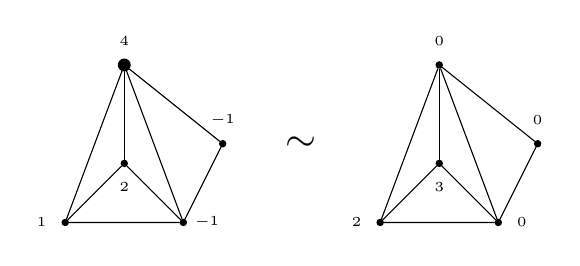
\begin{tikzpicture}
\node[circle,fill=black,inner sep=0.8pt,draw] (a) at (0,0) {};
\node[circle,fill=black,inner sep=0.8pt,draw] (b) at (1.5,0) {};
\node[circle,fill=black,inner sep=1.5pt,draw] (c) at (.75,2) {};
\node[circle,fill=black,inner sep=0.8pt,draw] (d) at (0.75,.75) {};
\node[circle,fill=black,inner sep=0.8pt,draw] (e) at (2,1) {};


\node () at (-0.3,0) {\tiny$1$};
\node () at (0.75,0.45) {\tiny$2$};
\node () at (0.75,2.3) {\tiny$4$};
\node () at (2,1.3) {\tiny$-1$};
\node () at (1.8,0) {\tiny$-1$};

\draw (a)--(b)--(e)--(c) --(a)--(d)--(b)--(c);
\draw (c)--(d);

\node at (3,1) {\Large{$\sim$}};

\begin{scope}[shift={(+4,0)}]
\node[circle,fill=black,inner sep=0.8pt,draw] (a) at (0,0) {};
\node[circle,fill=black,inner sep=0.8pt,draw] (b) at (1.5,0) {};
\node[circle,fill=black,inner sep=0.8pt,draw] (c) at (.75,2) {};
\node[circle,fill=black,inner sep=0.8pt,draw] (d) at (0.75,.75) {};
\node[circle,fill=black,inner sep=0.8pt,draw] (e) at (2,1) {};


\node () at (-0.3,0) {\tiny$2$};
\node () at (0.75,0.45) {\tiny$3$};
\node () at (0.75,2.3) {\tiny$0$};
\node () at (2,1.3) {\tiny$0$};
\node () at (1.8,0) {\tiny$0$};

\draw (a)--(b)--(e)--(c) --(a)--(d)--(b)--(c);
\draw (c)--(d);

\end{scope}
\end{tikzpicture}
\captionof{figure}{The larger vertex fires once to move from the left configuration to the right configuration.}
\end{texexample}

Behind the scenes pgf uses the basic system command \docAuxCommand{pgfnode} to create the nodes. The syntax of the command is given on \seepgfmanual{1026} as:

\begin{docCommand}{pgfnode}{\marg{shape}\marg{anchor}\marg{label text}\marg{name}\marg{path usage command}}
This command creates a new node. The \marg{shape} of the node must have been declared previously using
\lstinline{pgfdeclareshape}.

The shape is shifted such that the \marg{anchor} is at the origin. In order to place the shape somewhere else,
use the coordinate transformation prior to calling this command.
The hnamei is a name for later reference. If no name is given, nothing will be “saved” for the node, it
will just be drawn.

The \marg{path usage command} is executed for the background and the foreground path (if the shape defines
them).
\end{docCommand}


A good workflow, is to first define the nodes, next label them and then draw any connecting lines.

\begin{texexample}{Named nodes}{ex:named} 
\begin{tikzpicture}
\node[circle,fill=black,inner sep=0.8pt,draw] (a) at (0,0) {};
\node[circle,fill=black,inner sep=0.8pt,draw] (b) at (1.5,0) {};
\node[circle,fill=black,inner sep=1.5pt,draw] (c) at (.75,2) {};
\node[circle,fill=black,inner sep=0.8pt,draw] (d) at (0.75,.75) {};
\node[circle,fill=black,inner sep=0.8pt,draw] (e) at (2,1) {};
\end{tikzpicture}
\end{texexample}

\begin{texexample}{Named nodes}{ex:named} 
\begin{tikzpicture}
\node[circle,fill=black,inner sep=0.8pt,draw] (a) at (0,0) {};
\node[circle,fill=black,inner sep=0.8pt,draw] (b) at (1.5,0) {};
\node[circle,fill=black,inner sep=1.5pt,draw] (c) at (.75,2) {};
\node[circle,fill=black,inner sep=0.8pt,draw] (d) at (0.75,.75) {};
\node[circle,fill=black,inner sep=0.8pt,draw] (e) at (2,1) {};
% absolute labelling
\node () at (-0.3,0) {\tiny$1$};
\node () at (0.75,0.45) {\tiny$2$};
\node () at (0.75,2.3) {\tiny$4$};
\node () at (2,1.3) {\tiny$-1$};
\node () at (1.8,0) {\tiny$-1$};
\end{tikzpicture}
\end{texexample}

\begin{texexample}{Named nodes}{ex:named} 
\begin{tikzpicture}
\pgfdeclarelayer{background}
\pgfdeclarelayer{foreground}
\pgfsetlayers{background,main,foreground}
\node[circle,fill=black,inner sep=0.8pt,draw] (a) at (0,0) {};
\node[circle,fill=black,inner sep=0.8pt,draw] (b) at (1.5,0) {};
\node[circle,fill=black,inner sep=1.5pt,draw] (c) at (.75,2) {};
\node[circle,fill=black,inner sep=0.8pt,draw] (d) at (0.75,.75) {};
\node[circle,fill=black,inner sep=0.8pt,draw] (e) at (2,1) {};
% absolute labelling
\node () at (-0.3,0) {\tiny$1$};
\node () at (0.75,0.45) {\tiny$2$};
\node () at (0.75,2.3) {\tiny$4$};
\node () at (2,1.3) {\tiny$-1$};
\node () at (1.8,0) {\tiny$-1$};
% draw connecting lines
\draw (a)--(b)--(e)--(c) --(a)--(d)--(b)--(c);
\draw (c)--(d);
%\begin{pgfonlayer}{background}
\begin{scope}[on background layer={color=blue!10}]
\node [fill=blue!10,fit=(a) (b) (c)
(d) (e)] {};
\end{scope}
%\end{pgfonlayer}
\end{tikzpicture}
\end{texexample}

Just to recap, using \docAuxCommand*{node} and the \textbf{at} we can position accurately any node. We could have used the much longer command |path node|, but in our case above this is unecessary (\seepgfmanual{49}), for more explanations if you are still unsure.

Nodes can be named or unnamed. There are two ways to name them, with the key \docValue{name} or within brackets. The second method is to be preferred. Names for nodes can be pretty arbitrary, but they should not contain commas, periods, parentheses, colons, and some other special characters. However, they can contain underscores and hyphens

\subsection{Layers and Scope}

We can add a backround layer, using the library \textit{backgrounds}, which provides key values for adding backgrounds. \pgfname\ provides a layering mechanism for composing graphics from
multiple layers. (This mechanism is not to be confused with the
conceptual ``software layers'' the \pgfname\ system is composed of.)
Layers are often used in graphic programs. The idea is that you can
draw on the different layers in any order. So you might start drawing
something on the ``background'' layer, then something on the
``foreground'' layer, then something on the ``middle'' layer, and then
something on the background layer once more, and so on. At the end, no
matter in which ordering you drew on the different layers, the layers
are ``stacked on top of each other'' in a fixed ordering to produce
the final picture. Thus, anything drawn on the middle layer would come
on top of everything of the background layer.

Normally, you do not need to use different layers since you will have
little trouble ``ordering'' your graphic commands in such a way that
layers are superfluous. However, in certain situations you only
``know'' what you should draw behind something else after the
``something else'' has been drawn.

For example, suppose you wish to draw a yellow background behind your
picture. The background should be as large as the bounding box of the
picture, plus a little border. If you know the size of the bounding box
of the picture at its beginning, this is easy to accomplish. However,
in general this is not the case and you need to create a
``background'' layer in addition to the standard ``main'' layer. Then,
at the end of the picture, when the bounding box has been established,
you can add a rectangle of the appropriate size to the picture.

\subsection{Declaring Layers}

In \pgfname\ layers are referenced using names. The standard layer,
which is a bit special in certain ways, is called |main|. If nothing
else is specified, all graphic commands are added to the |main|
layer. You can declare a new layer using the following command:

\begin{docCommand}{pgfdeclarelayer}{\marg{name}}
  This command declares a layer named \meta{name} for later
  use. Mainly, this will set up some internal bookkeeping.
\end{docCommand}

The next step toward using a layer is to tell \pgfname\ which layers
will be part of the actual picture and which will be their
ordering. Thus, it is possible to have more layers declared than are
actually used.

\begin{docCommand}{pgfsetlayers}{\marg{layer list}}
  This command tells \pgfname\ which layers will be used in
  pictures. They are stacked on top of each other in the order
  given. The layer |main| should always be part of the list. Here is
  an example:
\begin{codeexample}[code only]
\pgfdeclarelayer{background}
\pgfdeclarelayer{foreground}  
\pgfsetlayers{background,main,foreground}
\end{codeexample}

  This command should be given either outside of any picture or ``directly inside'' of a picture.
  Here, the ``directly inside'' means that there should be no further level of \TeX\ grouping between |\pgfsetlayers| and the matching |\end{pgfpicture}| (no closing braces, no |\end{...}|). It will also work if |\pgfsetlayers| is provided before |\end{tikzpicture}| (with similar restrictions).
\end{docCommand}


\subsection{Using Layers}

Once the layers of your picture have been declared, you can start to
``fill'' them. As said before, all graphics commands are normally
added to the |main| layer. Using the |{pgfonlayer}| environment, you
can tell \pgfname\ that certain commands should, instead, be added to
the given layer.

\begin{docEnvironment}{pgfonlayer}{\marg{layer name}}
\end{docEnvironment}

The whole \meta{environment contents} is added to the layer with the
name \meta{layer name}. This environment can be used anywhere inside
a picture. Thus, even if it is used inside a |{pgfscope}| or a \TeX\
group, the contents will still be added to the ``whole'' picture.
Using this environment multiple times inside the same picture will
cause the \meta{environment contents} to accumulate.

  \emph{Note:} You can \emph{not} add anything to the |main| layer
  using this environment. The only way to add anything to the main
  layer is to give graphic commands outside all |{pgfonlayer}|
  environments. 



\begin{codeexample}[]
\pgfdeclarelayer{background layer}
\pgfdeclarelayer{foreground layer}
\pgfsetlayers{background layer,main,foreground layer}
\begin{tikzpicture}
  % On main layer:
  \fill[blue] (0,0) circle (1cm);
  
  \begin{pgfonlayer}{background layer}
    \fill[yellow] (-1,-1) rectangle (1,1);
  \end{pgfonlayer}
  
  \begin{pgfonlayer}{foreground layer}
    \node[white] {foreground};
  \end{pgfonlayer}
  
  \begin{pgfonlayer}{background layer}
    \fill[black] (-.8,-.8) rectangle (.8,.8);
  \end{pgfonlayer}

  % On main layer again:
  \fill[blue!50] (-.5,-1) rectangle (.5,1);
\end{tikzpicture}
\end{codeexample}



\long\gdef\mytriangle{
\node[circle,fill=black,inner sep=0.8pt,draw] (a) at (0,0) {};
\node[circle,fill=black,inner sep=0.8pt,draw] (b) at (1.5,0) {};
\node[circle,fill=black,inner sep=1.5pt,draw] (c) at (.75,2) {};
\node[circle,fill=black,inner sep=0.8pt,draw] (d) at (0.75,.75) {};
\node[circle,fill=black,inner sep=0.8pt,draw] (e) at (2,1) {};
% absolute labelling
\node () at (-0.3,0) {\tiny$1$};
\node () at (0.75,0.45) {\tiny$2$};
\node () at (0.75,2.3) {\tiny$4$};
\node () at (2,1.3) {\tiny$-1$};
\node () at (1.8,0) {\tiny$-1$};
% draw connecting lines
\draw (a)--(b)--(e)--(c) --(a)--(d)--(b)--(c);
\draw (c)--(d);
}

\begin{texexample}{Adding backgrouns}{ex:backgrounds}
\begin{tikzpicture}
\pgfdeclarelayer{background}
\pgfdeclarelayer{foreground}
\pgfsetlayers{background,main,foreground}
\mytriangle
%\begin{pgfonlayer}{background}
\begin{scope}[on background layer={color=blue!10}]
\mytriangle
\node [fill=blue!10,fit=(a) (b) (c)
(d) (e)] {};
\end{scope}
%\end{pgfonlayer}
\end{tikzpicture}
\end{texexample}


\begin{texexample}{Adding backgrouns}{ex:backgrounds}
\begin{tikzpicture}
\pgfdeclarelayer{background}
\pgfdeclarelayer{foreground}
\pgfsetlayers{background,main,foreground}
\mytriangle
%\begin{pgfonlayer}{background}
\begin{scope}[on background layer={color=blue!10}]
\node [fill=blue!10,fit=(a) (b) (c)
(d) (e)] {};
\end{scope}

\begin{scope}[shift={(+4,0)}]
\mytriangle
\begin{pgfonlayer}{background}
\node [pattern=checkerboard light gray,fit=(a) (b) (c)
(d) (e)] {};
\end{pgfonlayer}
\end{scope}
\end{tikzpicture}
\end{texexample}

This brings us to the end of our discussion. Time for a coffee and a break.                

\section{Adding styles}

In our previous example, we cut and pasted many of the repetitive keys. \pgfname offers a way to set a new key to the values of other keys using the handler |.style|. This is a very powerful way of redefining new keys, but also simplifying the code. Styles in \tikzname can be considered similar to macros in standard LaTeX. When I made a drawing, we can still tweak the styles and look how the drawing changes, until it's perfect. You should never have to tweak each node.

\begin{texexample}{Using styles}{ex:usingstyles}
\tikzset{BN/.style = {circle,fill=black,inner sep=0.8pt,draw},
         tiny/.style = {font=\tiny}, 
}
\begin{tikzpicture}
\node[BN] (a) at (0,0) {};
\node[BN] (b) at (1,0) {};
\node[BN] (c) at (1,1) {};
\node[BN] (d) at (0,1) {};
\node[BN] (e) at (-1,0) {};

\node () at (-1.3,0) [tiny]{$v_1$};
\node () at (-.3,1)  [tiny]{$v_2$};
\node () at (1.3,0)  [tiny]{$w_1$};
\node () at (1.3,1)  [tiny]{$w_2$};

\node[tiny] () at (0.5,-0.2) {$a$};
\node[tiny] () at (0.5,1.2) {$b$};
\node[tiny] () at (0.2,0.5) {$c$};
\node[tiny] () at (-0.5,-.2) {$d$};

\draw (e) -- (a) -- (b) -- (c) -- (d) -- (a);
\draw (e) -- (d);

\end{tikzpicture}
\end{texexample}



\section{Arcs and options for lines}

\begin{texexample}{Draw a Line}{ex:line}
\begin{tikzpicture}
\draw[->] (0,0) -- (1.5,0) node[draw, ellipse] {First Node} -| (0, 1.2) node[draw,ellipse,rotate=45] {Second Node};
\end{tikzpicture}
\end{texexample}

\begin{texexample}{Drawing arcs}{ex:matharcs}
We define 
\begin{gather*}
    \bar{d}_{k,l}:=\hspace{6pt}
    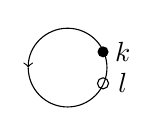
\begin{tikzpicture}[baseline=(current bounding box.center)]
    \draw[->] (3,2) arc (-180:180:5mm);
	  \fill (3.95,2.2) circle [radius=2pt];
    \draw (3.95,1.8) circle [radius=2pt];
    \node at (4.2,1.8) {$l$};
    \node at (4.2,2.2) {$k$};
    \end{tikzpicture}
    \hspace{0.5cm}
    \text{and}
    \hspace{0.5cm}
    d_{k,l}:=\hspace{6pt}
    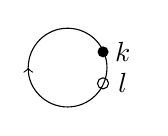
\begin{tikzpicture}[baseline=(current bounding box.center)]
    \draw[<-] (3,2) arc (-180:180:5mm);
    \fill (3.95,2.2) circle [radius=2pt];
    \draw (3.95,1.8) circle [radius=2pt];
    \node at (4.2,1.8) {$l$};
    \node at (4.2,2.2) {$k$};
    \end{tikzpicture}
    \hspace{0.5cm}
    \text{for}
    \hspace{2mm} k,l\in\mathbb{Z}_{\geq 0}.
\end{gather*}
\end{texexample}


Here is a figure that you should try and reproduce.
\newcommand{\G}{\Gamma}

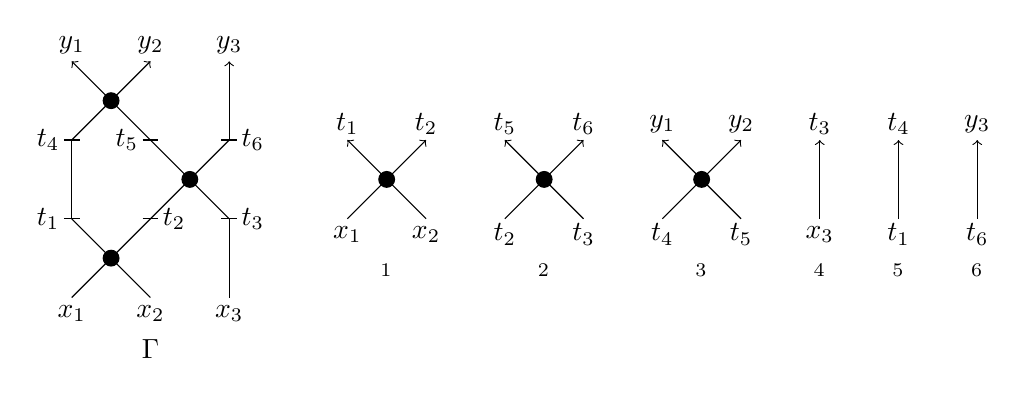
\begin{tikzpicture}
\draw (-3.5,-1)--(-2.5,0); \draw (-2.5,-1)--(-3.5,0); \draw (-1.5,-1)--(-1.5,0);\draw[fill=black] (-3,-0.5) circle (0.1cm); \draw (-3.5,0)--(-3.5,1); \draw (-2.5,0)--(-1.5,1); \draw (-1.5,0)--(-2.5,1);\draw[fill=black] (-2,0.5) circle (0.1cm); \draw[->] (-3.5,1)--(-2.5,2); \draw[->] (-2.5,1)--(-3.5,2); \draw[->] (-1.5,1)--(-1.5,2); \draw[fill=black] (-3,1.5) circle (0.1cm); \draw (-3.6,0)--(-3.4,0);\draw (-2.6,0)--(-2.4,0);\draw (-1.6,0)--(-1.4,0); \draw (-3.6,1)--(-3.4,1);\draw (-2.6,1)--(-2.4,1);\draw (-1.6,1)--(-1.4,1); \node at (-3.5,-1.2) {$x_1$};\node at (-2.5,-1.2) {$x_2$};\node at (-1.5,-1.2) {$x_3$}; \node at (-3.5,2.2) {$y_1$};\node at (-2.5,2.2) {$y_2$};\node at (-1.5,2.2) {$y_3$}; \node at (-3.8,0) {$t_1$};\node at (-2.2,0) {$t_2$};\node at (-1.2,0) {$t_3$}; \node at (-3.8,1) {$t_4$};\node at (-2.8,1) {$t_5$};\node at (-1.2,1) {$t_6$}; \node at (-2.5,-1.65) {$\Gamma$};
\draw[->] (0,0)--(1,1); \draw[->] (1,0)--(0,1); \draw[fill=black] (0.5,0.5) circle (0.1cm); \draw[->] (2,0)--(3,1); \draw[->] (3,0)--(2,1); \draw[fill=black] (2.5,0.5) circle (0.1cm); \draw[->] (4,0)--(5,1); \draw[->] (5,0)--(4,1); \draw[fill=black] (4.5,0.5) circle (0.1cm); \draw[->] (6,0)--(6,1); \draw[->] (7,0)--(7,1); \draw[->] (8,0)--(8,1);
\node at (0,-.2) {$x_1$};\node at (1,-.2) {$x_2$}; \node at (2,-.2) {$t_2$};\node at (3,-.2) {$t_3$}; \node at (4,-.2) {$t_4$};\node at (5,-.2) {$t_5$}; \node at (6,-.2) {$x_3$}; \node at (7,-.2) {$t_1$}; \node at (8,-.2) {$t_6$};
\node at (0,1.2) {$t_1$};\node at (1,1.2) {$t_2$}; \node at (2,1.2) {$t_5$};\node at (3,1.2) {$t_6$}; \node at (4,1.2) {$y_1$};\node at (5,1.2) {$y_2$}; \node at (6,1.2) {$t_3$}; \node at (7,1.2) {$t_4$}; \node at (8,1.2) {$y_3$};
\node at (0.5,-0.65) {$\G_1$}; \node at (2.5,-0.65) {$\G_2$}; \node at (4.5,-0.65) {$\G_3$}; \node at (6,-0.65) {$\G_4$};\node at (7,-0.65) {$\G_5$};\node at (8,-0.65) {$\G_6$}; 
\end{tikzpicture}

This brings us to the end.




The |node| can take numerous options who are then used to set the typesetting of the text that follows:


\begin{texexample}{Draw a Line}{ex:line}
\begin{tikzpicture}
\draw[->] (0,0) -- (1.5,0) node[draw, ellipse] {First Node} -| (0, 1.2) node[draw,ellipse,rotate=45, text width=3cm, fill=creamy, text justified] {\lorem};
\end{tikzpicture}
\end{texexample}


\begin{texexample}{Draw a Line}{ex:line}
\begin{tikzpicture}[funny ellipse/.style = {draw,ellipse,rotate=45, text width=3cm, fill=creamy, text justified} ]
\draw[->] (0,0) -- (1.5,0) node[draw, ellipse] {First Node} -| (0, 1.2) node[funny ellipse] {\lorem};
\end{tikzpicture}
\end{texexample}

This can also be written by using \docAuxCommand{tikzset} for setting out all the keys. This can written just before the environment or within the scope of the environment. See \href{https://tex.stackexchange.com/questions/52372/should-tikzset-or-tikzstyle-be-used-to-define-tikz-styles}{TX.SX discussion}, for the option to set |\tikzstyle| which should not be used, even if it is quicker to write.


\begin{texexample}{Draw a Line}{ex:line}
\tikzset{funny ellipse/.style = {draw,ellipse,rotate=45, text width=3cm, fill=creamy, text justified} }
\begin{tikzpicture}
\draw[->] (0,0) -- (1.5,0) node[draw, ellipse] {First Node} -| (0, 1.2) node[funny ellipse] {\lorem};
\end{tikzpicture}
\end{texexample}

A |node| can possibly be rendered with a choice from a list of over 720 keys.

ed. 



Using the |TikZ| package you can draw figures and intermingle them with text. To draw a simple diamond as shown in \fref{fig:diamond} we use
the following commands. The package comes with a very comprehensive manual of over 500 pages long. One can state that there is nothing that you cannot draw with PGF/TikZ, if you have the patience and perseverance. TikZ's language has a syntax of its own with very little connection to what we have used so far. You will need to set aside adequate time to study this, especially if your work has a lot of specially drawn figures that you need. The result like anything else in \tex make the effort worthwhile.

\begin{texexample}{Draw a Diamond}{fig:diamond}
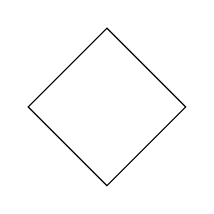
\begin{tikzpicture}
 \draw (1,0) -- (0,1) -- (-1,0) -- (0,-1) -- cycle;
\end{tikzpicture}
\end{texexample}


\begin{texexample}{Text long path}{ex:decorations}
\begin{tikzpicture}
\draw [help lines] grid (3,2);
\draw [red, dashed]
[postaction={decoration={text along path, text={a big juicy apple},
text align=fit to path}, decorate}]
(0,0) .. controls (0,2) and (3,2) .. (3,0);
\node (A) at (1.5,0) {!};
\end{tikzpicture}
\end{texexample}


\begin{texexample}{Text long path}{ex:decorations}

Hello \begin{pgfpicture}
\pgfpathrectangle{\pgfpointorigin}{\pgfpoint{2ex}{1ex}}
\pgfusepath{stroke}
\end{pgfpicture} World!

\end{texexample}


\emphasis{-,draw,begin,end,tikzpicture}
\begin{teXXX}
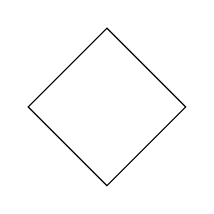
\begin{tikzpicture}
\draw (1,0) -- (0,1) -- (-1,0) -- (0,-1) -- cycle;
\end{tikzpicture}
\end{teXXX}



\makeatletter
The value of $x$ is \pgfsys@markposition{here}important.

Lots of text.
\hbox{\pgfsys@markposition{myorigin}%
\begin{pgfpicture}
% Switch of size protocol
\pgfpathmoveto{\pgfpointorigin}
\pgfusepath{use as bounding box}
\pgfsys@getposition{here}{\hereposition}
\pgfsys@getposition{myorigin}{\thispictureposition}
\pgftransformshift{\pgfpointscale{-1}{\thispictureposition}}
\pgftransformshift{\hereposition}
\pgfpathcircle{\pgfpointorigin}{1cm}
\pgfusepath{draw}
\end{pgfpicture}}

\makeatother


You cannot write directly into a picture environment. The command \docAuxCommand{pgftext} can be used. 

\begin{texexample}{Using text directly}{ex:pgftext}
\tikz{\draw[help lines] (0,0) grid (3,2);
\pgftext[base,x=1cm,y=0.5cm] {lovely}}
\end{texexample}





Sometimes it is quite useful when debugging to add a backround grid. 


\begin{centering}
\begin{tikzpicture}
\draw[step=0.25cm,color=creamy] (-1,-1) grid (1,1);
\draw [color=bgsexy](1,0) -- (0,1) -- (-1,0) -- (0,-1) -- cycle;
\end{tikzpicture}
\captionof{figure}{You can add a background grid using \texttt{step=0.25cm, color=green} as an option}
\end{centering}


\emphasis{step,color,green,grid,begin,end}
\begin{teXXX}
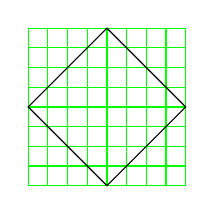
\begin{tikzpicture}
  \draw[step=0.25cm,color=green] (-1,-1) grid (1,1);
  \draw (1,0) -- (0,1) -- (-1,0) -- (0,-1) -- cycle;
\end{tikzpicture}
\end{teXXX}

The grid is specified by providing two diagonally opposing points: (-1,-1)
and (1, 1). The two options supplied give a step size for the grid lines and a
specification for the color of the grid lines, using the \docpkg{xcolor} package

\subsection{Specifying points and paths}

\begin{texexample}{Specifying points and paths}{ex:points}
\centering
\begin{tikzpicture}[scale=1.8]
% Define the points of a regular pentagon
\path (0,0) coordinate (origin);
\path (0:1cm) coordinate (P0);
\path (1*72:1cm) coordinate (P1);
\path (2*72:1cm) coordinate (P2);
\path (3*72:1cm) coordinate (P3);
\path (4*72:1cm) coordinate (P4);
% Draw the edges of the pentagon
\draw[color=bgsexy] (P0) -- (P1) -- (P2) -- (P3) -- (P4) -- cycle;
% Add "spokes"
\draw[color=bgsexy] (origin) -- (P0) (origin) -- (P1) (origin) -- (P2)
(origin) -- (P3) (origin) -- (P4);
\end{tikzpicture}
\captionof{figure}{Drawing a complicated polygon, using paths and the \texttt{draw} command}
\end{texexample}


Two key ideas used in \tikzname\ are points and paths. Both of these ideas were used
in the diamond examples. Much more is possible, however. For example, points
can be specified in any of the following ways:
\begin{enumerate}
\item  Cartesian coordinates
\item  Polar coordinates
\item  Named points
\item  Relative points
\end{enumerate}



\subsection{coordinates}
The cartesian coordinates can be defined and named using the following syntax.

%\emphasis{begin,end,coordinate,at,draw}
%\begin{teXXX}
%\begin{tikzpicture}
%  \coordinate (A) at (0,0);
%  \coordinate (B) at (1.25,0.25);
%  \draw[blue] (A) -- (B);
%\end{tikzpicture}
%\end{teXXX}

\noindent This produces:
\begin{tikzpicture}
\coordinate (A) at (0,0);
\coordinate (B) at (1.25,0.25);
\draw[blue] (A) -- (B);
\end{tikzpicture}


We can add labels to the points by using the |label| option. A label is distinct from the text of a |node|.

\begin{tikzpicture}
\coordinate [label=left:\textcolor{orange}{$A$}] (A) at (0,0);
\coordinate [label=right:\textcolor{orange}{$B$}]  (B) at (1.15,0.25);
\draw[blue] (A) -- (B);
\end{tikzpicture}

\emphasis{label,left,label:,right}
\begin{teXXX}
\begin{tikzpicture}
  \coordinate [label=left:\textcolor{orange}{$A$}] (A) at (0,0);
  \coordinate [label=west:\textcolor{orange}{$B$}] (B) at (1.25,0.25);
  \draw[blue] (A) -- (B);
\end{tikzpicture}
\end{teXXX}




If you tempted to write \texttt{label=top:} it will not work, as the command accepts the following keywords.


\begin{tikzpicture}
  \coordinate [label=left:\textcolor{orange}{east}]  (A) at (0,0);
  \coordinate [label=right:\textcolor{orange}{west}] (B) at (0,0);
  \draw[blue] (A)--(B);
\end{tikzpicture}


\section{Graphic Parameters: Line Width, Line Cap, and Line Join}

The width of lines can be specified using the key:

\begin{docKey}[tikz]{line width}{=\marg{dimension}} {no default, initially 0.4pt}
Specifies the line width \seepgfmanual{166}
\end{docKey}



\bgroup
\def\mkl#1{\tikz \draw[#1] (0,0)--(1.0, 1.5ex);}
\scriptsize\arial
\begin{tabular}{|l|l|l|l|l|l|l|l|}
\hline
\mkl{line width=2pt}& \mkl{ultra thin} &\mkl{very thin} & \mkl{thin} & \mkl{semithick} & \mkl{thick} &\mkl{very thick} &\mkl{ultra thick} \\
\hline
line width=2pt &ultra thin & very thin & thin &semithick & thick & very thick & ultra thick \\
\hline
\end{tabular}
\egroup

\begin{docKey}[tikz]{line cap}{=\marg{dimension}} {no default, initially 0.4pt}
Specifies how lines “end.” Permissible types are round, rect, and butt \seepgfmanual{167}. 
\end{docKey}

\bgroup
\def\mkl#1{\begin{tikzpicture} \draw[line width=10pt, line cap=#1] (0,0)--(1.0, 1.5ex);\draw[white,line width=2pt]
(0,0 )--(1.0,1.5ex);\end{tikzpicture}}
\scriptsize\arial
\begin{tabular}{|l|l|l|}
\hline
\mkl{rect}& \mkl{butt} &\mkl{round}  \\
\hline
rect &butt & round \\
\hline
\end{tabular}
\egroup




\begin{docKey}[tikz]{line join}{=\marg{type}}{no default, initially miter}
Specifies how lines “join.” Permissible type are round, bevel, and miter. They have the following
effects:
\end{docKey}

\begin{texexample}{Joining Lines}{es:joinlines}

\begin{tikzpicture}[line width=10pt]
\draw[line join=round] (0,0) -- ++(.5,1) -- ++(.5,-1);
\draw[line join=bevel] (1.25,0) -- ++(.5,1) -- ++(.5,-1);
\draw[line join=miter] (2.5,0) -- ++(.5,1) -- ++(.5,-1);
\end{tikzpicture}
\end{texexample}


\begin{docKey}[tikz]{dash pattern}{=\marg{dash pattern}}{no default}
Sets the dashing pattern. The syntax is the same as in \metafontlogo. For example following pattern on
2pt off 3pt on 4pt off 4pt means \enquote{draw 2pt, then leave out 3pt, then draw 4pt once more, then
leave out 4pt again, repeat}.
\end{docKey}

\bgroup
\def\ml#1{\tikz \draw[ #1] (0pt,0pt) -- (50pt,0pt);}
\def\alist{solid, dotted, densely dotted, loosely dotted,% 
           dashed,densely dashed, loosely dashed, %
           dash dot, densely dash dot, loosely dash dot, %
           dash dot dot, densely dash dot dot, loosely dash dot dot.}

For patterns there are numerous settings {\arial \alist }


\scriptsize
\begin{tabular}{lll}
\hline
\ml{solid} &  & \\
solid      &  & \\
\hline
\ml{dotted} &\ml{densely dotted} & \ml{loosely dotted}\\
\textit{dotted} & densely dotted  &loosely dotted \\
\hline
\ml{dashed} & \ml{densely dashed} & \ml{loosely dashed}  \\
\textit{dashed}      & densely dashed & loosely dashed            \\
\hline

\ml{dash dot} & \ml{densely dash dot} & \ml{loosely dash dot} \\
\textit{dash dot} & densely dash dot & loosely dash dot \\
\hline

\ml{dash dot dot} & \ml{densely dash dot dot} & \ml{loosely dash dot dot} \\
\textit{dash dot dot} & densely dash dot dot & loosely dash dot dot \\
\hline
\end{tabular}
\egroup


\subsection{Pattern Library}

The library patterns can be used to draw predetermined patterns. This will be a longer than usual section as it explains how to create new patterns. Most of the content is straight from the \pgfname manual. Before we start with the creation f a new pattern let us examine how a pattern is used.

\begin{texexample}{Using Library Patterns}{ex:libpatterns}
\begin{tikzpicture}
\pattern [path fading=west,pattern=checkerboard light gray]
      (0,0) rectangle (5cm,2em);
\end{tikzpicture}
\end{texexample}


\label{section-library-patterns}


The package defines patterns for filling areas. \docAuxCommand*{usetikzlibrary}\marg{patterns}.




\subsection{Form-Only Patterns}

\begin{tabular}{ll}
  \emph{Pattern name} & \emph{Example (pattern in black, blue, and red
    on faded checkerboard)} \\ 
  \patternindex{horizontal lines} 
  \patternindex{vertical lines} 
  \patternindex{north east lines} 
  \patternindex{north west lines} 
  \patternindex{grid} 
  \patternindex{crosshatch} 
  \patternindex{dots} 
  \patternindex{crosshatch dots} 
  \patternindex{fivepointed stars} 
  \patternindex{sixpointed stars} 
  \patternindex{bricks}
  \patternindex{checkerboard}
\end{tabular}
  
\subsection{Inherently Colored Patterns}


\begin{tabular}{ll}
  \emph{Pattern name} & \emph{Example} \\
  \patternindexinherentlycolored{checkerboard light gray} 
  \patternindexinherentlycolored{horizontal lines light gray} 
  \patternindexinherentlycolored{horizontal lines gray} 
  \patternindexinherentlycolored{horizontal lines dark gray} 
  \patternindexinherentlycolored{horizontal lines light blue} 
  \patternindexinherentlycolored{horizontal lines dark blue} 
  \patternindexinherentlycolored{crosshatch dots gray} 
  \patternindexinherentlycolored{crosshatch dots light steel blue} 
\end{tabular}
  


% Copyright 2006 by Till Tantau
%
% This file may be distributed and/or modified
%
% 1. under the LaTeX Project Public License and/or
% 2. under the GNU Free Documentation License.
%
% See the file doc/generic/pgf/licenses/LICENSE for more details.


\section{Creating Patterns}

\label{section-patterns}

\subsection{Overview}

There are many ways of filling a path. First, you can fill it using a
solid color and this is also the fastest method. Second, you can also
fill it using a shading, which means that the color changes smoothly
between two (or more) different colors. Third, you can fill it using a
tiling pattern and it is explained in the following how this is done.

A tiling pattern can be imagined as a rectangular tile (hence the
name) on which a small picture is painted. There is not a single tile,
but (conceptually) an infinite number of tiles, all showing the same
picture, and these tiles are arranged horizontally and vertically to
fill the plane. When you use a tiling pattern to fill a path, what
happens is that the path clips out a ``window'' through which we see
part of this infinite plane.

Patterns come in two versions: \emph{inherently colored patterns} and
\emph{form-only patterns}. (These are often called ``color patterns''
and ``uncolored patterns,'' but these names are misleading since
uncolored patterns do have a color and the color changes. As I said,
the name is misleading\dots) An inherently colored pattern is just a
colored tile like, say, a red star with a black outline. A form-only
pattern can be imagined as a tile that is a kind of rubber stamp. When
this pattern is used, the stamp is used to print copies of the stamp
picture onto the plane, but we can use a different stamp color each
time we use a form-only pattern.

\pgfname\ provides a special support for patterns. You can declare a
pattern and then use it very much like a fill color. \pgfname\
directly maps patterns to the pattern facilities of the underlying
graphic languages (PostScript, \textsc{pdf}, and \textsc{svg}). This
means that filling a path using a pattern will be nearly as fast as if
you used a uniform color.

There are a number of pitfalls and restrictions when using
patterns. First, once a pattern has been declared, you cannot change
it anymore. In particular, it is not possible to enlarge it or change
the line width. Such flexibility would require that the repeating of
the pattern were not done by the graphic language, but on the
\pgfname\ level. This would make patterns orders of magnitude slower
to produce and to render. However, \pgfname{} does provide a
more-or-less successful emulation of ``mutable'' patterns, although
internally, a new (fixed) instance of a pattern is declared when
the parameters of a pattern change.

Second, the phase of patterns is not well-defined, that is, it is not
clear where the origin of the ``first'' tile is. To be more precise,
PostScript and \textsc{pdf} on the one hand and \textsc{svg} on the
other hand define the origin differently. PostScript and \textsc{pdf}
define a fixed origin that is independent of where the path lies. This
has the highly desirable effect that if you use the same pattern to
fill multiple paths, the outcome is the same as if you had filled a 
single path consisting of the union of all these paths. By
comparison, \textsc{svg} uses the upper-left (?) corner of the path to
be filled as the origin. However, the \textsc{svg} specification is a
bit vague on this question.


\subsection{Declaring a Pattern}

Before a pattern can be used, it must be declared. The following
command is used for this:

\begin{docCommand}{pgfdeclarepatternformonly}{%
	\oarg{variables}%
	\marg{name}%
	\marg{bottom left}%
	\marg{top right}%
	\marg{tile size}%
	\marg{code}}

	This command declares a new form-only pattern. The \meta{name} is a
  name for later reference. The two parameters \meta{lower left} and
  \meta{upper right} must describe a bounding box that is large enough
  to encompass the complete tile.
\end{docCommand}

  The size of a tile is given by \meta{tile size}, that is, a tile is
  a rectangle whose lower left   corner is the origin and whose upper
  right corner is given by \meta{tile size}. This might make you
  wonder why the second and third parameters are needed. First, the
  bounding box might be smaller than the tile size if the tile is
  larger than the picture on the tile. Second, the bounding box might
  be bigger, in which case the picture will ``bleed'' over the tile.

  The \meta{code} should be \pgfname\ code than can be protocolled. It
  should not contain any color code.


\begin{codeexample}[]
\pgfdeclarepatternformonly{stars}
{\pgfpointorigin}{\pgfpoint{1cm}{1cm}}
{\pgfpoint{1cm}{1cm}}
{
  \pgftransformshift{\pgfpoint{.5cm}{.5cm}}
  \pgfpathmoveto{\pgfpointpolar{0}{4mm}}
  \pgfpathlineto{\pgfpointpolar{144}{4mm}}
  \pgfpathlineto{\pgfpointpolar{288}{4mm}}
  \pgfpathlineto{\pgfpointpolar{72}{4mm}}
  \pgfpathlineto{\pgfpointpolar{216}{4mm}}
  \pgfpathclose%
  \pgfusepath{fill}
}
\begin{tikzpicture}
  \filldraw[pattern=stars] (0,0)   rectangle (1.5,2);
  \filldraw[pattern=stars,pattern color=red]
                           (1.5,0) rectangle (3,2);
\end{tikzpicture}
\end{codeexample}

	The optional argument \meta{variables} consists of a comma
	separated	list of macros,	registers or keys, representing the
	parameters of the pattern that may vary. If a variable is a key,
	then the full path name must be used (specifically, it must start
	with |/|).
	As an example, a list might look like the following:
	|\mymacro,\mydimen,/pgf/my key|. Note that macros and keys should
	be ``simple''. They should only store values in themselves.
	
	The effect of \meta{variables}, is the following:
  Normally, when this argument is empty, once a pattern has been
  declared, it becomes ``frozen''. This means that it is not possible
  to enlarge the pattern or change the line width later on.
  By specifying \meta{variables}, no pattern is actually created.
  Instead, the arguments are stored away
  (so the macros,	registers or keys do not have to be defined in advance).

  When the fill pattern is set, \pgfname{} checks if the pattern has
  already been created with the \meta{variables} set to their current
  values (\pgfname{} is usually ``smart enough'' to distinguish between
  macros, registers and keys). If so, this already-declared-pattern
  is used as the fill pattern.
  If not, a new instance of the pattern (which will have a
  unique internal name) is declared using the current values of
  \meta{variables}. These values are then saved and the fill pattern
  set accordingly.
	
	The following shows an example of a pattern which varies
	according to the values of the macro |\size|, the key |/tikz/radius|,
	and the \TeX{} dimension |\thickness|.

\begin{texexample}{New Pattern Example}{ex:newpattern}
\pgfdeclarepatternformonly[/tikz/radius,\thickness,\size]{rings}
{\pgfpoint{-0.5*\size}{-0.5*\size}}
{\pgfpoint{0.5*\size}{0.5*\size}}
{\pgfpoint{\size}{\size}}
{
  \pgfsetlinewidth{\thickness}
  \pgfpathcircle\pgfpointorigin{\pgfkeysvalueof{/tikz/radius}}
  \pgfusepath{stroke}
}
\newdimen\thickness
\tikzset{
  radius/.initial=4pt,
  size/.store in=\size, size=20pt,
  thickness/.code={\thickness=#1},
  thickness=0.75pt
}
\begin{tikzpicture}[rings/.style={pattern=rings}]
  \filldraw [rings, radius=2pt, size=6pt]      (0,0)   rectangle +(1.5,2);
  \filldraw [rings, radius=2pt, size=8pt]      (2,0)   rectangle +(1.5,2);
  \filldraw [rings, radius=6pt, thickness=2pt] (0,2.5) rectangle +(1.5,2);
  \filldraw [rings, radius=8pt, thickness=4pt] (2,2.5) rectangle +(1.5,2);
\end{tikzpicture}
\end{texexample}



\begin{docCommand}{pgfdeclarepatterninherentlycolored}{\oarg{variables}
    \marg{name}
    \marg{lower left}
    \marg{upper right}
    \marg{tile size}
    \marg{code}}
  This command works like |\pgfdeclarepatternuncolored|, only the
  pattern will have an inherent color. To set the color, you should
  use \pgfname's color commands, not the |\color| command, since this
  fill is not protocolled.
\end{docCommand}

\begin{texexample}{Inherently Colored}{ex:ingerentlycolored}
\pgfdeclarepatterninherentlycolored{green stars}
{\pgfpointorigin}{\pgfpoint{1cm}{1cm}}
{\pgfpoint{1cm}{1cm}}
{
  \pgfsetfillcolor{green!50!black}
  \pgftransformshift{\pgfpoint{.5cm}{.5cm}}
  \pgfpathmoveto{\pgfpointpolar{0}{4mm}}
  \pgfpathlineto{\pgfpointpolar{144}{4mm}}
  \pgfpathlineto{\pgfpointpolar{288}{4mm}}
  \pgfpathlineto{\pgfpointpolar{72}{4mm}}
  \pgfpathlineto{\pgfpointpolar{216}{4mm}}
  \pgfpathclose%
  \pgfusepath{stroke,fill}
}
\begin{tikzpicture}
  \filldraw[pattern=green stars] (0,0) rectangle (3,2);
\end{tikzpicture}
\end{texexample}



\subsection{Setting a Pattern}

Once a pattern has been declared, it can be used.

\begin{docCommand}{pgfsetfillpattern}{\marg{name}\marg{color}}
  This command specifies that paths that are filled should be filled
  with the ``color'' by the pattern \meta{name}. For an inherently
  colored pattern, the \meta{color} parameter is ignored. For
  form-only patterns, the \meta{color} parameter specifies the color
  to be used for the pattern.
\end{docCommand}
  
\begin{codeexample}[]
\begin{tikzpicture}
  \pgfsetfillpattern{stars}{red}
  \filldraw (0,0) rectangle (1.5,2);

  \pgfsetfillpattern{green stars}{red}
  \filldraw (1.5,0) rectangle (3,2);
\end{tikzpicture}
\end{codeexample}



\endinput
%To summarize, what we have been doing so far is to learn a set of primitive TikZ commands for drawing paths, drawing shapes and labeling them. All TikZ command work by passing options to them. For example to change the above line to an arrow, we just pass the option |->| to the |draw| command.
%

%\begin{tikzpicture}
%  \coordinate [label=left:\textcolor{orange}{$A$}] (A) at (0,0);
%  \coordinate [label=right:\textcolor{orange}{$B$}] (B) at (1.25,0.25);
%  \draw[->,o-stealth] (A)--(B);
%\end{tikzpicture}
%\caption{Effect of the option \protect\texttt{draw[->]}.}

%\emphasis{begin,end,->,draw}
%\begin{teXXX}
%\begin{tikzpicture}
%  ...
%  ...
%  \draw[->,blue] (A)--(B);
%\end{tikzpicture}
%\end{teXXX}
%
%\section*{Relative coordinates}
%\index{TikZ!coordinates, relative}
%A coordinate can be made "relative" by prefixing it with |++|. relative coordinates are useful in many applications.
%\medskip
%
%\noindent The code is simple, except before the coordinate you add the |++| signs. This tells the PGF engine to add the x,y dimensions of the new coordinate to that of its predecessor's. In many instances this is more intuitive and easier to determine.



%\begin{tikzpicture}
%\draw[step=0.5cm,color=gray] (-1,-1) grid (3.5,3);
%\draw[->,red,thick] (0,0) -- ++(1,0) -- ++(0,1) -- ++(-1,0) -- cycle;
%\draw[->,red,thick] (2,0) -- ++(1,0) -- ++(0,1) -- ++(-1,0) -- cycle;
%\draw[arrows=o-stealth,blue] (1.5,1.5) -- ++(1,0) -- ++(0,1) -- ++(-1,0) -- cycle;
%\end{tikzpicture}
%\caption{Example of use of the \protect\texttt{++} to specify relative coordinates.}
%\label{fig:relative}

%\begin{teXXX}
%\begin{tikzpicture}
%  \draw[step=0.5cm,color=gray] (-1,-1) grid (3.5,3);
%  \draw[red,very thick] (0,0) -- ++(1,0) -- ++(0,1) -- ++(-1,0) -- cycle;
%  \draw[red,very thick] (2,0) -- ++(1,0) -- ++(0,1) -- ++(-1,0) -- cycle;
%  \draw[->,red,very thick] (1.5,1.5) -- ++(1,0) -- ++(0,1) -- ++(-1,0) -- cycle;
%\end{tikzpicture}
%\end{teXXX}
%
%Instead of |++| you can also use a single |+|. This also specifies a relative coordinate, but it does not "update"
%the current point for subsequent usages of relative coordinates. Thus, you can use this notation to specify
%numerous points, all relative to the same "initial" point:
%

%\begin{tikzpicture}
%\draw[step=0.5cm,color=gray] (-1,-1) grid (3.5,3);
%\draw[purple, fill=white] (0,0) -- +(1,0) -- +(1,1) -- +(0,1) -- cycle;
%\draw[purple, fill=white] (2,0) -- +(1,0) -- +(1,1) -- +(0,1) -- cycle;
%\draw[purple, fill=white] (1.5,1.5) -- +(1,0) -- +(1,1) -- +(0,1) -- cycle;
%\path (0,0) node [shape=circle,draw]{(0,0)};
%\end{tikzpicture}
%\caption{Example of use of the \protect\texttt{+} to specify relative coordinates.}
%\label{fig:relative1}

%\begin{teXXX}
%  \draw (0,0) -- +(1,0) -- +(1,1) -- +(0,1) -- cycle;
%  \draw (2,0) -- +(1,0) -- +(1,1) -- +(0,1) -- cycle;
%  \draw (1.5,1.5) -- +(1,0) -- +(1,1) -- +(0,1) -- cycle;
%\end{teXXX}
%
%
%Personally, I don't favour this method of specifying co-ordinates, but it can be useful, if you are automating the production of figures through an external script\sidenote{For drawing Bezier curves, the \texttt{+} behaves differently.  You can refer to the PGF Manual for more details.}.
%
%
%\section*{Arrows}
%\index{TikZ>arrows}
%The function |->| creates a tooltip arrow. You can use different arrow tips and there is a long section for them in the PGF manual. You can even define your own.

\bgroup
%\centering
%\begin{tikzpicture}
%  \draw[->] (0,0) -- (2,0);
%  \draw[arrows=o-stealth,blue] (0,-0.3) -- (2,-0.3);
%  \draw[->,o-stealth,orange] (0,-0.6) -- (2,-0.6);
%  \draw[arrows=|-stealth,purple] (0,-0.9) -- (2,-0.9);
%\end{tikzpicture}
%\captionof{figure}{Special arrow endings}
%\label{fig:specials}
\egroup
%
%\emphasis{o,stealth,begin,end,draw}
%\begin{teXXX}
%\begin{tikzpicture}
% \draw[->] (0,0) -- (2,0);
% \draw[arrows=o-stealth,blue] (0,-0.3) -- (2,-0.3);
% \draw[->,o-stealth,orange] (0,-0.6) -- (2,-0.6);
% \draw[arrows=X-stealth,purple] (0,-0.9) -- (2,-0.9);
%\end{tikzpicture}
%\end{teXXX}

%

\begin{verbatim}
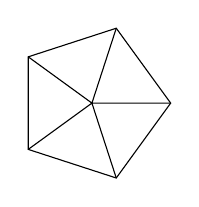
\begin{tikzpicture}
% Define the points of a regular pentagon
\path (0,0) coordinate (origin);
\path (0:1cm) coordinate (P0);
\path (1*72:1cm) coordinate (P1);
\path (2*72:1cm) coordinate (P2);
\path (3*72:1cm) coordinate (P3);
\path (4*72:1cm) coordinate (P4);
% Draw the edges of the pentagon
\draw (P0) -- (P1) -- (P2) -- (P3) -- (P4) -- cycle;
% Add "spokes"
\draw (origin) -- (P0) (origin) -- (P1) (origin) -- (P2)
(origin) -- (P3) (origin) -- (P4);
\end{tikzpicture}
\end{verbatim}





\section{Nodes}

A node is a small part of a picture. When a node is created, you provide a position where the node
should be drawn and a shape. A node of shape circle will be drawn as a |circle|, a node of shape |rectangle|
as a rectangle, and so on. A node may also contain same text, which is why they can used nodes to show text.

Finally, a node can get a name for later reference.



\emphasis{node,shape,draw}
\begin{teXXX}
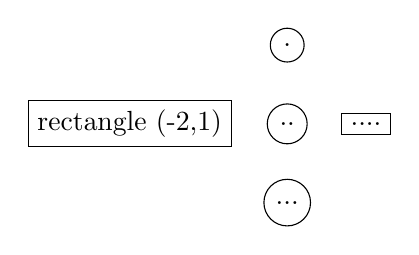
\begin{tikzpicture}
\path ( 0,2) node [shape=circle,draw] {.}
( 0,1) node [shape=circle,draw] {..}
( 0,0) node [shape=circle,draw] {...}
( 1,1) node [shape=rectangle,draw] {....}
(-2,1) node [shape=rectangle,draw] {rectangle (-2,1)};
\end{tikzpicture}
\end{teXXX}
\medskip

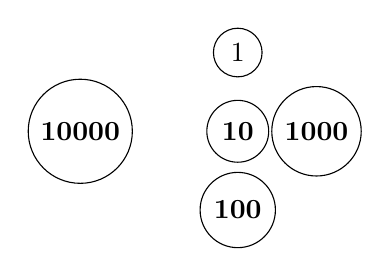
\begin{tikzpicture}
\path ( 0,2) node [shape=circle,draw] {1}
( 0,1) node [shape=circle,draw] {\textbf{10}}
( 0,0) node [shape=circle,draw] {\textbf{100}}
( 1,1) node [shape=circle,draw] {\textbf{1000}}
(-2,1) node [shape=circle,draw] {\textbf{10000}};
\end{tikzpicture}

In the above code, this text is empty (because of the
|empty {}|). So, why do we see anything at all at all the nodes? The answer is the draw option for the node operation: It
causes the |shape| around the text" to be drawn. If you have an empty |{}|, PGF still sees the empty space as a character and justs draws around it. The reason is than TikZ automatically adds some space around the text. The amount is set
using the option |inner sep|. So, to increase the size of the nodes. Modifying the example slightly we get.



\begin{tikzpicture}
\path ( 0,2) node [shape=circle,draw] {.}
( 0,1) node [shape=circle,draw] {..}
( 0,0) node [shape=circle,draw] {...}
( 1,1) node [shape=circle,draw] {....}
(-1,1) node [shape=circle,draw] {.....};
\end{tikzpicture}

As you can observe the size of the circle has been adjusted to fit the text that is enclosing it. 
Another way to simply add a node is using the |at| syntax:

\begin{texexample}{The node command}{}
\begin{tikzpicture}
\node at (0,0) [circle, draw] {\textbf{100}};
\node at (1,1) [diamond,draw] {\textbf{100}};
\end{tikzpicture}
\end{texexample}

The \cmd{\node} is an abbreviation of the |\path| node. This is a much shorter syntax than |\path| where one would need to add a lot of redundant move-tos  \seepgfmanual{215}.

If you have many nodes another way of achieving the example outlined above is to use the |\draw| command in comination with node and at.

\begin{texexample}{The node command}{}
\begin{tikzpicture}
\tikz \draw[fill=yellow!80!black]
(0,0) node {first node}
-- (1,1) node[draw, behind path] {second node}
-- (0,2) node[fill=red!20,draw,double,rounded corners] {third node};

\node at (0,0) [circle, draw] {\textbf{100}};
\node at (1,1) [diamond,draw]{\textbf{100}};
\end{tikzpicture}
\end{texexample}

\subsection*{Drawing shapes}

PGF abd \tikzname\ come with a number of predefined shapes:
\begin{itemize}
\item rectangle
\item circle, and
\item coordinate
\end{itemize}


\begin{tikzpicture}
\draw (0,0) circle (1cm);
\draw (0.5,0) circle (0.5cm);
\draw (0,0.5) circle (0.5cm);
\draw (-0.5,0) circle (0.5cm);
\draw (0,-0.5) circle (0.5cm);
\end{tikzpicture}



A circle is specified by providing its center point and the desired radius. The
command:

\medskip

\begin{tikzpicture}
  \draw[step=0.25cm,color=green] (-1,-1) grid (1,1);
  \draw (0,0) circle (1cm);
\end{tikzpicture}
\medskip

\begin{teXXX}
\begin{tikzpicture}
  \draw (x,y) circle (dia);
\end{tikzpicture}
\end{teXXX}



You  can use one |\draw| command to draw multiple circles as shown in \fref{fig:circles}


\begin{tikzpicture} 
 \draw (0,0) 
  circle (1cm)
  circle (0.6cm)
  circle (0.2cm)
 ;
\end{tikzpicture}

\emphasis{circle,begin,end}
\begin{teXXX}
\begin{tikzpicture} 
 \draw (0,0) 
  circle (1cm)
  circle (0.6cm)
  circle (0.2cm)
 ;
\end{tikzpicture}
\end{teXXX}





\begin{center}
\begin{tikzpicture}
\draw (0,0) circle (1cm)
circle (0.6cm)
circle (0.2cm);
\end{tikzpicture}
\captionof{figure}{You can use one draw command to draw multiple circles}
\label{fig:circles}
\end{center}
\captionof{figure}{Drawing multiple circles, using mutiple \texttt{circle} commands}


\subsection{Drawing ellipses}

Ellipses can be drawn in a similar fashion to circles. As an ellipse needs two center points to be specified the command used has the following general form:

\begin{verbatim}
\draw (a,b) ellipse (r1 dim and r2 dim);
\end{verbatim}

We can draw two ellipses as shown in the figure, using the code:
\begin{teX}
\begin{tikzpicture}[scale=0.6]
\draw[color=red] (0,0) ellipse (2cm and 1cm);
\draw[color=red] (0,0) ellipse (1cm and 2cm);
\end{tikzpicture}
\end{teX}

\begin{centering}
\begin{tikzpicture}[scale=0.6]
\draw[color=red] (0,0) ellipse (2cm and 1cm);
\draw[color=red] (0,0) ellipse (1cm and 2cm);
\end{tikzpicture}
\caption[Drawing ellipses]{Use the draw command in combination with ellipse to draw ellipses}
\end{centering}


\begin{teX}
\begin{tikzpicture}
\draw (0,0) ellipse (2cm and 1cm)
ellipse (0.5cm and 1 cm)
ellipse (0.5cm and 0.25cm);
\end{tikzpicture}
\caption{Drawing multiple circles, using mutiple \texttt{draw} commands}
\end{teX}

\section{Drawing more complicated shapes}
we can place a parabola in a rectangle as shown in \fref{fig:parabola}, by using the |rectangle| and the |parabola| options.

\bgroup
\centering

\begin{tikzpicture}
\draw[color=blue] (0,0) rectangle (1,1.5)
(0,0) parabola[color=orange] (1,1.5);
\draw[xshift=1.5cm] (0,0) rectangle (1,1.5)
(0,0) parabola[bend at end] (1,1.5);
\draw[xshift=3cm] (0,0) rectangle (1,1.5)
(0,0) parabola bend (.75,1.75) (1,1.5);
\end{tikzpicture}
\captionof{figure}{Parabolas drawn using the parabola and rectangle options.}
\label{fig:parabola}
\egroup




\emphasis{parabola,rectangle}
\begin{teX}
\begin{tikzpicture}
\draw[color=blue] (0,0) rectangle (1,1.5)
(0,0) parabola[color=orange] (1,1.5);
\draw[xshift=1.5cm] (0,0) rectangle (1,1.5)
(0,0) parabola[bend at end] (1,1.5);
\draw[xshift=3cm] (0,0) rectangle (1,1.5)
(0,0) parabola bend (.75,1.75) (1,1.5);
\end{tikzpicture}
\caption{Parabolas drawn using the parabola command}
\label{fig:parabola}
\end{teX}

\subsection*{The shape library}

\begin{tikzpicture}
\draw [help lines] (0,0) grid (2,2);
\draw [blue, dashed] (1,1) circle(1cm);
\draw [red, dashed] (1,1) circle(.5cm);
\node [star, star point height=.5cm, minimum size=2cm, draw]
at (1,1) {S};
\end{tikzpicture}

\section{Iterations}
One convenient construct provided with TikZ is a |foreach| command sequence

\begin{texexample}{Tikz loops}{tz:ex}
\centering
\begin{tikzpicture}[scale=2, color=bgsexy]
\foreach \i in {1,...,4}
{
  \path (\i,0) coordinate (X\i);
  \fill (X\i) circle (1pt);
}
  \foreach \j in {1,...,3}
{
  \path (\j,1) coordinate (Y\j);
  \fill (Y\j) circle (1pt);
}
\foreach \i in {1,...,4}
{
  \foreach \j in {1,...,3}
  {
     \draw[color=bgsexy] (X\i) -- (Y\j);
  }
}
\end{tikzpicture}
\captionof{figure}{Drawing a bi-partite garph using foreach loops}
\end{texexample}



\section{The pgfplots package}



\subsection{Loading data from files}

Scientific work, especially that associated with research tends to generate
a lot of data. The data would normally come from external applications and stored in files. With |TikZ| one can import the data
by using the word |file|:

\emphasis{addplot,file,x}
\begin{teXXX}
 \addplot file {./raw/wavefunctions/wavefunc\x.dat};
\end{teXXX}

In the example we use a file with a path. The data is saved in
files with the same name but a different ending. We use a |foreach| function to add the ending i.e, the file names are |wavefunc1|, |wavefunc2| and |wavefunc3|. By using external data files and the foreach command it can substantially reduce the amount of text in the macros. This improves debugging and readability.

\begin{texexample}[colback=white]{Loading files}{ex:lfiles}
\centering
\begin{tikzpicture}[scale=0.8]
    \begin{axis}[smooth,
    xlabel=$n$,
    ylabel=$\Theta{j}{n}$]
    \foreach \x in {0,...,2}
    {
        \addplot file {./raw/wavefunctions/wavefunc\x.dat};
    }
    \legend{$j=0$,$j=1$,$j=2$};
    \end{axis}
\end{tikzpicture}
\captionof{figure}{Example plot with data imported from external files, using \texttt{file}}
\end{texexample}


\begin{teXXX}
\begin{tikzpicture}[scale=0.6]
  \begin{axis}[
    xlabel=$n$,
    ylabel=$\Theta{j}{n}$]
    \foreach \x in {0,...,2}
    {
      \addplot file {./raw/wavefunctions/wavefunc\x.dat};
    }
    \legend{$j=0$,$j=1$,$j=2$};
  \end{axis}
\end{tikzpicture}
\end{teXXX}



\section*{Plotting functions}
Functions can be defined for plotting using a variety of methods. They are powerful but generally difficult to remember.



\section{Saving Data to a file}

You can save your data to a file in many ways. One easy way is to use
the \docpkg{filecontents} package. This package extends the LaTeX environment
with the same name, but allows you to overwrite the file {\protect\ctan{filecontents}}.

\begin{teXXX}
\documentclass[justified]{tufte-book}
\usepackage{pgfplots,lipsum,booktabs}
\usepackage{pgfplotstable}
\pgfplotsset{compat=newest}
\usepackage{filecontents*}
\begin{filecontents}{my1.dat}
    Label       value       num
    Integrity     33         4
    Standalone    14         3
    Interface      6         2
    Overall       18         1
\end{filecontents*}
\begin{document}
    your code here ...
\end{document}
\end{teXXX}

It is good practice to keep, such data at the top of your file, although with
the |filecontents| package, they can be inserted anywhere. Sometimes it maybe
easier to have a number of minimal files with the type of charts you using regularly and just update the data on top. In general if the data is entered
by hand rather than generated automatically by software this is a good way
to keep your work tidy.

\newenvironment{Chart}[1][black!70!green]{%
%%  defaults
    \gdef\level##1{Level ##1}
    \def\setchartwidth##1{%
      \def\chartwidth{##1}}%
    \setchartwidth{3.9cm}%
    \def\chartcolor{#1}
    \newcommand\addTitle[2][test]{
    
    
%% For the chart title we set it in a minipage for
%% better control
    \def\charttitle{\minipage{4cm}%
       \footnotesize %
       \centering\textbf{##2}\\##1%
       \endminipage}}%
   \def\xlabel{Completion (\%)}%
%% renders the chart 
    \def\renderChart{%
%%
    \footnotesize%
%%
%%
    \IfFileExists{#1.dat}{Test}{}
   \begin{tikzpicture}
   \begin{axis}[
    xbar, width=\chartwidth,title=\charttitle,
    y=0.5cm, enlarge y limits={true, abs value=0.75},
    xmin=0, xmax=100,enlarge x limits={upper, value=0.25},
    xlabel=\xlabel,
    %ylabel=Label,
    xmajorgrids=true,
    ytick=data,
    yticklabels from table={\dataTable}{Label},
    nodes near coords, nodes near coords align=horizontal
     ]
    \addplot[draw=none, fill=\chartcolor] table [x=value, y=num]
    {\dataTable};
    \end{axis}%
    \end{tikzpicture}}}
{}

\begin{comment}
\begin{figure*}
\centering

\hskip-2cm\begin{Chart}
 \addTitle[Mechanical Systems]{Shangri-la}
 \def\dataTable{SH-mechanical.dat}
 \renderChart
\end{Chart}\hspace{0.3cm}
\begin{Chart}
 \addTitle[FM-200 System]{All areas}
 \def\dataTable{my1.dat}
 \renderChart
\end{Chart}
\begin{Chart}
 \addTitle[Electrical Works]{Merweb}
 \def\dataTable{my6.dat}
 \renderChart
\end{Chart}
\caption{Mechanical Systems Shangrila. Commissioning status}
\end{figure*}


\begin{filecontents*}{my1.dat}
Label     value       num
Integrity         33            4
Standalone      14            3
Interface        6            2
Overall           18            1
\end{filecontents*}

\begin{filecontents*}{SH-mechanical.dat}
Label     value       num
{Fan coil units}       43             8
{Air Handling Units}       13             7 
{CW Pumps}       13             6
{ECU}       11             5
{Pressurization Fans}        15             4
{Smoke Extract Fan}       5             3
{Jet fan}       5             2
{Overall}       12              1
\end{filecontents*}

\begin{filecontents*}{my6.dat}
Label    value         num   other
{Level 7}  50           11   13
L6         90           10   12
L5       80             9    16
L4       90             8    18
L3       70             7    90
L2       80             6    21
L1       70             5    22
\end{filecontents*}

\begin{filecontents*}{carparkventilation.dat}
Label    value         num   other
L5         50           11   13
L4         90           10   12
L3         80           9    16
GR         90           8    18
B1         70           7    90
B2         80           6    21
B3         70           5    22
\end{filecontents*}
%% CO SYSTEM
%% DATA
\begin{filecontents*}{carparkco.dat}
Label    value         num   other
L5         78           7   13
L4         90           6   12
L3         80           5    16
GR         90           4    18
B1         70           3    90
B2         80           2    21
B3         70           1    22
B5         50          {}    {}
\end{filecontents*}

\begin{filecontents*}{carparkco2.dat}
value,   num,   other,
78,       7,   13,
90,       6,   12,
80,       5,    16,
90,       4,    18,
70,       3,    90,
80,       2,    21,
70,       1,    22,
\end{filecontents*}
\end{comment}






















%%\def\chaptername{Chapter}
%\makeatletter
%\cxset{style13}
\cxset{style87a/.style={
 chapter opening=any,
 name=Chapter,
 % positioning and float - inline is 0
 %  float right is 2
 number display=block,
 number float=right,
 number shape=starburst,
 chapter numbering=arabic,
 number spaceout=none,
 number font-size=huge,
 number font-weight=mdseries,
 number font-family=sffamily,
 number font-shape=upshape,
 number before=,
 number display=inline,
 number float=none,
% 
 number border-top-width=0pt,
 number border-right-width=0pt,
 number border-bottom-width=0pt,
 number border-left-width=0pt,
 number border-width=0pt,
%  
 number padding-left=0em,
 number padding-right=0.5em,
 number padding-top=0em,
 number padding-bottom=0pt,
  %number margin-top=, to do
 %number margin-left=0pt,  to create
 %
 number after=,
 number dot=,
 number position=rightname,
 number color=black,
 number background-color=white,
 %chapter name
 chapter display=block,
 chapter float=left,
 chapter shape=ellipse,
 chapter color=white,
 chapter background-color=sweet,
 chapter font-size= Huge,
 chapter font-weight=mdseries,
 chapter font-family=sffamily,
% chapter font-shape=upshape,
 chapter before=,
 chapter spaceout=none,
 chapter after=,
 chapter margin left=0cm,
 chapter margin top=0pt,
 %
 chapter border-width=0pt,
 chapter border-top-width=0pt,
 chapter border-right-width=0pt,
 chapter border-bottom-width=0pt,
 chapter border-left-width=0pt,
% 
 chapter padding-left=0pt,
 chapter padding-right=0pt,
 chapter padding-top=0pt,
 chapter padding-bottom=0pt,
  %chapter title
 title font-family=sffamily,
 title font-color=black!80,
 title font-weight=bfseries,
 title font-size=huge,
 chapter title align=none,
 title margin-left=1cm,
 title margin bottom=1.3cm,
 title margin top=25pt,
 % title borders
 title border-width=0pt,
 title padding=0pt,
 title border-color=black!80,
% title border-top-color=spot!50,
% title border-top-width=20pt,
 title border-left-color=black!80,
 title border-left-width=2pt,
 title border-color=black!80,
 title padding-top=10pt,
 title padding-bottom=10pt,
 title padding-left=10pt,
 title padding-right=0pt,
% title border-right-color=spot!50,
% title border-right-width=20pt,
% title border-bottom-color=spot!50,
% title border-bottom-width=20pt,
 %
 chapter title align=left,
 chapter title text-align=left,
 chapter title width=0.8\textwidth,
 title before=0pt,
 title after=,
 title display=block,
 title beforeskip=,
 title afterskip=,
 author block=false,
 section font-family=rmfamily,
 section font-size=LARGE,
 section font-weight=bfseries,
 section indent=0pt,
 epigraph width=\dimexpr(\textwidth-2cm)\relax,
 epigraph align=center,
 epigraph text align=center,
 section color=spot!50,
 section font-weight=bfseries,
 section align=left,
 section number after=\hskip10pt,
 section font-family=sffamily,
 section numbering prefix=\@arabic\c@chapter.,
 epigraph rule width=0pt,
 header style=plain}}
 \makeatother
 
\cxset{style87a}


\cxset{ 
           %chapter toc=true,
           chapter numbering=arabic,
           chapter number color=black,
           chapter number font-shape=upshape,
           subsubsection numbering=none,
           subsubsection font-family=itshape,
           subsubsection color=black,
           subsection number after=\quad,
          section number after=\quad,
          section color=black,
    }
\def\thesubsubsection{}         
%\pagenumbering{gobble}
\def\JV{HLS DSE-JV\xspace}
\def\letter#1{\texttt{HLSDSEJV/HC/L/YL/#1}\xspace}
\def\KA{K\&A}
\def\DT#1{HLG Transmittal Ref. No.: \texttt{HLG-626-DT-HLS-#1}\xspace}
\def\idxbusbar#1{\index{Busbar Delays>#1}}
\def\idxwestin#1{\index{Westin Delays>#1}}
\def\idxstregis#1{\index{St. Regis Delays>#1}}
\def\idxahu#1{\index{Air Handling Unit Delays>#1}}
\let\idxahus\idxahu
\def\CAR#1{\index{Cost Adjustment Requests>CAR-#1}{\texttt{CAR-#1}}\xspace}
\def\idxbasement#1{\index{Basement delays>#1}}
\let\basement\idxbasement
\def\idxdewa#1{\index{Dewa Approvals>#1}}


\mainmatter
\pagestyle{plain}
\cxset{chapter name=,
          chapter numbering=none}
\chapter{Executive Summary}
\thispagestyle{empty}

This short report provides background information related to  the Habtoor City Project MEP works and the steps taken by the \JV to accelerate the works, under the instructions of the Client, Engineer and Main Contractor.  We mobilized to the Project late August 2013. At the time construction was on-going, with the basements structures mostly completed. On mobilization the only K\&A MEP designs available were those provided with the tender package---which was issued in March~2013. Besides procurement and some engineering activities, the \JV  construction activities were mainly focused on builder's works and remaining underground services until March 2014. 

We started receiving design drawings in March and April 2014. The design was issued piecemeal and in out of sequence fashion for the works to progress as planned and according to the agreed Baseline Program . This enabled us to proceed with works only in the Car Parking Areas of the Basements.  The first partially workable set of design drawings received to enable construction in other areas were the drawings received in September 2014 (Mechanical) and December 2014 (Electrical).


\medskip
		
\paragraph{Delayed Incomplete and Unworkable MEP Designs} The general issue of drawings in September~14, provided general design concepts without concerns for physical plant and ceiling constraints. The Plant rooms at T1 and PD6, as designed were not constructible, as the allocated headroom and space was inadequate. We assisted the Engineer by providing 3D and other drawings to at least fit the equipment in the available space. Fans had to be relocated in ceilings at Podium 1, and ducting was re-routed over the same ceiling void. This delayed finalization of Shop Drawings for essentially all the public areas.


The K\&A \enquote{design} mechanical design for St. Regis was only partially completed in September 2014. This design was deficient in many respects, especially in areas such the Technical floors, and as it stood the design was not constructible. This design was inadequate to close equipment orders for long delivery plant, such as AHU, fans and pumps, as calculations for static pressures could not progress. However, we took the initiative to finalize orders based on estimates and released orders before design finalization. We also assisted the Engineer with solving many of the design issues in order to progress with the works.  In addition the Electrical works suffered because of the designs issued in September 2014, as they have not been co-ordinated with the requirements of the Mechanical plant, Kitchen Contractors etc. \par

The delays  to the completion of the final Project requirements are still on-going with many areas of the Hotels still under design development and without related subcontractors appointed on time.

\begin{table}[ht]
\centering

\begin{tabular}{l l p{3cm}  l l}
\toprule
        &Area         &\raggedright Design required as per baseline program & Design Issued & Delay\\
\midrule        
\inc  &First Floor &16 Apr 14  &5 Jan 15  &  8 months\\
\inc  &Attic Floor & 8 Apr 14  &5 Jan 15  & 8 months \\
\inc  &Podium 6  &1 Apr 14   &6 Sep 14  & 5 months \\
\inc  &Podium 5  &29 Mar 14 &6 Sep 14  & 5 months\\
\inc &Podium 4   &20 Mar 14 &6 Sep 14  & 5.5 months\\
\inc &Podium 3  &12 Mar 14  &6 Sep 14  & 5.5 months\\
\inc &Technical 1 &6 Feb 14   &6Sep 14    &7 months\\
\inc &Mezzanine &26 Dec 13  &6 Sep 14  &9 months\\ 
\bottomrule
\end{tabular}
\caption{Design delays for St. Regis}

\end{table}

The MEP Good for Engineering Designs as received from K\&A enabled part of the Engineering and Procurement activities to start bu the design as it stood was  proceed, they are not sufficient to install MEP services. Drawings from ID Consultants, Lighting Consultants, Kitchen Consultant, ELV Consultants and subcontractor Shop Drawings for the same are necessary. These were mostly unavailable.

\paragraph{Instruction to accelerate the works}
Under this background we received the instruction to  accelerate the works (July 2014). We wrote to to the Main Contractor, requesting that a plan be first agreed as to how program recovery could be achieved and \emph{then} agree to a plan to accelerate the works further, so as to bring the Contract Completion dates forward. The request was to accelerate the St. Regis Hotel first with a Target Completion date of 30 March 2014.

At the time approximately 40\% of the slabs  for St. Regis were incomplete. This included critical plant areas at the two technical floors. Not only the structure had to be completed, but also the technical floor, had to have floating floors casted. The T1 floor was partially handed over to us end October and the PD6 floor in January 2015. As is also evident from the subsequently issued Design MEP Drawings, ID Drawings, Lighting Consultant and ELV Consultant drawings issued, the Professional Team was not ready with their Designs. 

As MEP works are closely interlinked with other trades it is important to note that the Structure Cabling, Kitchen Subcontractors, AV and CCTV Subcontractors were not appointed. 
\medskip

 
   


\label{acceleration}
\index{acceleration>manpower}\index{manpower>acceleration}
\paragraph{JV actions taken to accelerate the works.} Once the information started flowing, we reinforced our Engineering and Site Teams. We also added technicians as areas opened to us for work.
\medskip

\noindent\textit{Workforce}
\medskip

\noindent The \JV upon receipt of the instructions to accelerate, and under the impression that designs and appointments of other subcontractors would be accelerated as well, doubled the workforce in July~2014 and subsequently added technicians and other staff until it is at its current level of approximately 3000 personnel. The deployment of personnel is shown in the table below.

\begin{table}[hbp]
\begin{tabular}{c c c c c c c c c}
\toprule
Item &Sep 13 &Feb 14 &Mar 14 & Jul-14 & Aug-14 &Oct-14 & Jan-15 & Mar-15\\
\midrule
 Site Labour   & 48      &610      & 634     & 1212   &  1300     & 1845   &2 781   & 2 731 \\
\bottomrule
\end{tabular}
\end{table}

Although issues prohibited us from fully handing over areas and ceiling closures, the quantum of the work achieved in this short time can be gauged from the gross claimed amount of close to AED~280,000,000.00. (April~14-April~15). 
\medskip

\noindent\textit{Air-freighting of equipment}
\medskip

\noindent In addition to adding personnel we proceeded to air-freight the following equipment, without which the program recovery would have failed:

\begin{enumerate}
\item Chilled water pumps. The chilled water pumps were necessary to be delivered as early as possible in order to enable piping to be connected and for providing wild air as possible. The first submittal for pumps was made on the 25 February 2014. This was returned on the 26 March 2014. The pumps were again resubmitted in 23 April 2014, after revisions to match changes in equipment. They were returned after 40 days, despite the fact that at the time the Engineer was asking us to accelerate the works. Third and fourth submittals followed and the pumps finally approved on 3 July 2014. Pump heads were reverified to meet new layouts and the order place in August, after opening LCs and finalizing prices with Supplier. Cost AED 50,000.00. 
\index{airfreight>chilled water pumps}
\index{chilled water pumps>air freight costs}

\item First fan coil units deliveries for St Regis. These were subjected to similar delays and 388 fan coil units were air-freighted from Thailand at a cost of 196,539.60~AED. 

\item Air Separator for the St Regis Plantroom was air-freighted at a cost of AED~14,185.00.
\item All fans for St Regis. Many of these fans were to be installed in ceiling voids. These were air-freighted at a cost of AED~221,772.00. This also included air-freighting charges for fire rated motors to be air-freighted from Brazil to the Nuaire Wales factory.

\item The above secured the St Regis Hotel plant room areas.

\item Air-freighting of ECUs and Basement fans was stopped after Client Representative wrote us a letter that they would not consider paying for the above costs. \index{Ecology Units>air freight} \index{air freight costs}

These were sea-freighted, with a consequent further compression in the program of works and delaying completion of the following areas:

\begin{enumerate}
\item Basement areas
\item PD6 St Regis Plantroom
\item Kitchens
\end{enumerate}
\end{enumerate}


These are also expected to delay commissioning of kitchen areas in the basement and the Car Park Ventilation System.

\paragraph{Focus of the claim}

The claim should focus on the following:

\begin{enumerate}
\item Establishing the time extension claim. This should not be too difficult given the delays in design information. Also the casting on all buildings had considerable delays (recorded in the weekly  reports). The biggest delays in casting occured in the "W" hotel. Considerable delays in the issue of provisional sums information was another source of delay. These are listed in the last section of this report. Engineering has all the details as to when the information was released to us. I have recorded the dates we required the information in order not to incur delays.

\item Establishing disruption. Unless this element can be argued successfully, the monetary claim will be insignificant. We should at least try and recover 20\% on the labour component.

\item Establishing acceleration. The Site Team needs to provide the Claim Consultant's an accurate status of the Project and details as to what is still incomplete. Please give attention to teh fact that there are two  non-binding contractual milestones. the completion of basement works and teh completion of the St. Regis Hotel by July 2015. These milestones need to be achieved in order to validate the acceleration part of the claim.
\end{enumerate}

Between the above three components we should be able to Claim in excess of  AED 30 million, which hopefully would recover the higher labour costs incurred.

The Sections that follow are general outlines and an incomplete list of what can be claimed. 
Full information is available with the Engineering Team and the Commercial Team.

\setcounter{chapter}{0}





%\chapter{Summary MEP Progress Report for St Regis Hotel, Habtoor City}
%\pagenumbering{arabic}
%\thispagestyle{plain}
%\section{Current Status}
%
%We have started flushing of the Chilled Water system on the 7 April 2015, as planned and we anticipate to be in a position to progressively provide \emph{wild air} before the end of April, ahead of the scheduled date of the 7 May 2015. In the Basements and in the Guest rooms we have started final fix works, where possible. The Main Plantrooms at Technical Floors 1 and Podium 6, are in the main completed, except final ductwork connections where they impede access. BMS DDC Panels are expected to arrive by the 22 April 2015 and installation expected to be completed within 25-30 days to ensure that by end May we can provide controlled conditions.
%
%Delays have been experienced in the receipt of Electrical panels, such as DBs (delayed due to late deliveries of components by Legrand) and others that were subjected to numerous changes, as described later on.  Other delays were due to late instructions as briefly detailed in Section~\ref{delays}. 
%
%The current outstanding works for the St Regis Hotel are as follows:
%
%\subsection{St Regis Basement}
%
%\begin{description}
%\item[Kitchen Corridors] Some kitchen corridors cable pulling is still under progress. Expected to complete by 30 Apr 2015.
%\item[Main Electrical Room] Delays experienced due to the failure of cable trays during cable pulling and also due to the some of the MDBs being returned to the factory for modifications, as they failed QA/QC Inspections.
%\item[Fan Rooms] Fans scheduled to be delivered 23 Apr 2015.
%\item[BMS] DDC Panels still to be delivered.
%\item[Sump Pumps] Expected to be delivered by 10 May 2015. 
%\item[Others] There are still closure related works, for areas currently inaccessible, such as the new ramp areas, store and office areas. 
%\end{description}
%
%\subsection{Ground Floor}
%\begin{description}
%\item[Ballroom] This area is still under scaffolding being used by the Main Contractor to erect walk-ways in the ceiling. Once the scaffolding is dropped and we are given access to the lower level, we have to install another layer of services, give ceiling grid clearances and upon construction of the ceiling grid we can then install final sprinkler droppers and give clearances for final boarding.
%\item[Banquet Hall] This area has been delayed due to the Iridium Spa delays in Design and appointment of subcontractors. As this area is above the Banquet Hall, coring for drainage pipes delayed the works. This coring is now complete and we expect to ask the Main Contractor to lower the scaffolding and start with the rest of the services.
%\end{description}
%\subsection{Mezzanine}
%\begin{description}
%\item[Festival Dining Restaurant] Currently this area is under nomination, there is no ID Design and final details are still awaited. 
%\item[Security Room] The design for this room has recently changed. The room as shown in the new designs is different from what has been constructed on site and has no space for CCUs. 
%\item[AV Room] Expected to be completed 30 Apr 2015.
%\item[Furniture Store] Expected to be completed 25 Apr 2015.
%\item[Balance Corridors] Expected to be completed 25 Apr 2015.
%\end{description}
%
%\subsection{Podium 1}
%
%\begin{description}
%\item[Banquet A/V Technician] We have no access. This is currently being used as a store.
%\item[Service Corridor] Plan to release for ceiling grid on 23 Apr 2015.
%\item[St Regis Main Kitchen and Corridor] Plan to release on 30 Apr 2015.
%\item[Property Store] Currently no access. If access provided we can release by 30 Apr 2015.
%\item[Steak House Kitchen] Plan to release by 30 Apr 2014.
%\end{description}
%
%\subsection{Podium 2}
%\begin{description}
%\item[Iridium Spa and related areas] We are currently working in the area, which was delayed by late appointment of Finishing Contractor. Still some ID Shop Drawings not available. We expect to catch-up with delays by end May 2015. We plan to complete final fix by 10 June 2015 and Testing and Commissioning by 20 Jul 2015.
%\item[Other Areas] All other areas will be released for closure by 26 Apr 2015.
%\end{description}
%
%\subsection{Podium 3-6}
%
%All guestrooms have been handed over for ceiling closures with the exception of some of the suites, where information and access was provided late. These are the following:
%
%\begin{description}
%\item[Ambassador Suite] Co-ordination ongoing. Expect resolution and final clearances 25 May 2015.
%\item[Bentley Suite] Incomplete information. Completion targets uncertain at this stage.
%\item[Royal Suite] Co-ordination on-going. Expect resolution and final clearances 25 May 2015.
%\end{description}
%
%\subsection{Floor 1}
%
%\begin{description}
%\item[Kitchen 4 and Kitchen 6] Works for walls are progressing, insufficient detail information. Can complete by 15 May 2015, provided all Kitchen Subcontactor’s drawings become available and unimpeded access.
%\end{description}
%
%\section{Delays in Target Dates}
%\label{delays}
%This is a brief summary of recent selected instructions for additional works that have impacted  MEP Progress. 
%In addition to these additional works another critical factor that affected progress was the congestion of services and the numerous RFIs and responses we had to raise in order to resolve them.
%
%\begin{itemize}
%\item Relocation of Kitchen Extract ducting Ground Floor, Mezzanine and Podium BOH areas.
%\item  Additional AV points in all public areas.
%\item  Additional telephone, data and CCTV points in all Public Areas.
%\item  Motorized curtains Meeting Rooms.
%\item Lighting Control System. 
%\item Emergency Lighting System. (see details Chapter~\ref{emergencylights})
%\item Changes to Electrical DBs, SMDBs due to late receipt of DEWA approved drawings. (See Chapter~\ref{electrical})
%\end{itemize}
%
%We have reacted as fast as possible to all instructions and as soon they were received we have added resources to mitigate delays. Where days slipped these are only by a few days and we are confident that by end of this month all physical installations will be completed with the exception of the English Pub, Banquet and Royal Suite. 
%
%\subsection{Back of the House Areas}
%
%All back of the House Areas experienced delays, due to the lack of primary co-ordination at design stage. This caused delays until solutions were found enabling us to install the services. 
%
%The allowable ceiling height in this area was impossible to be achieved and the kitchen extract duct eventually was split in two sections and distributed through two different routes in order to avoid passing it through the corridors which could not accomodate it.
%
%In addition a new roller shutter window was introduced, that made it impossible to install the fresh air ducts feeding the kitchen. After several attempts by |K&A| to find an acceptable solution the roller shutter  window was abandoned as per the instructions of the Client Representative. 
%
%\subsection{Basement Kitchen and Related Areas at B1}
%
%Please note that these areas (with the exception of the corridor) have been cleared for ceiling grid closures in most areas and the balances are as per target to close by the 15 April 2015, including additional works. The additional works were mostly for additional ELV points on walls and for which we have received drawings on the 29 March 2015. We have instituted overtime and added additional crews to complete the works as fast as possible. Most rooms in the area have been affected. 

\begin{comment}
\chapter{Busbar System}

As per the approved Baseline Program we expected to place the busbar order for all three hotels on 27 February 2014. However, HLS DSE-JV were unable to place any orders due to the events that are outlined below, with finality on all busbars only achieved in April 2015. 

\begin{enumerate}
\item On the 23 December 2013 we were requested to change the specification for some busbars via HLG transmittal Ref. No. HLG-626-DT-HLS-0628 dated 23 Decemeber 2013 \textit{Fire Resistance Bus Bar Specification}.

\item On the 25 February 2014 we were issued revised designs via tranmittal Ref. No. HLG-626-DT-HLS-0873 \textit{Revised Electrical Drawings}.

\end{enumerate}


\chapter{Generators}

\section{Generator Ventilation}

\subsection{Background}

The original tender drawings indicated the Generator Ventilation to be by means of Louvres. When such an approach is taken normally the ventilation openings are dictated by the size of the generators.


HLS DSE-JV have submitted as early as 2014 RFIs outlining concerns regarding the adequacy of the ventilation openings and sizing of Generator rooms in the basements.

On the 25 March 2015, we were instructed to proceed with the purchase of additional fans from Systemaire. We issued the order request on the ..... and the order placed on the ......  without formal approval of the amounts in order to speed up the purchase. This affected the commissioning of the generators.

\chapter{Transformer Room Ventilation}

\subsection{Background}

\subsection{Design Errors}
\end{comment}


\cxset{chapter name=Section,
          chapter numbering=arabic}
\chapter{Emergency Lighting System}
\label{emergencylights}
The Emergency Lighting System was finalized on the 22 February 2015. This is impacting on the final fix and commissioning of the Hotel’s Central Battery and Emergency Lighting System. 

\begin{enumerate}
\item As per the approved Baseline Program, we were planning to submit the Material Submission of the Emergency Lighting System by the 25 Feb 2014.
\item On the 25 Nov 2013, we raised RFI \texttt{HLS-DSE/142 JV-RFI-MEP-E028} requesting full details of the Emergency Lights as well as the capacity of the central battery system in order to proceed with Technical Submittals, design of containment system and procurement of equipment.
\item On the 12 Dec 2013 we received an insufficient reply to the above mentioned RFI. We have notified you that the repsonse was insufficient via letter \texttt{HLS DSE/JV/HLG/YL1181} dated 14 Jan 2014, clearly stating that we were unable to proceed further with the submission of the Central Battery System, until the requested information was provided. In our letter we had requested that all details such as diffuser details, base type, IP rating and lamp characteristics are provided. We have also provided details as to Civil Defence requirements.
\item The above concerns were forwarded to the Engineer by the Main Contractor on the 20 Jan 2014. The Engineer instructed us to follow the current design dawings until the completion of the Lighting Consultant’s works.

\item On 10 Feb 2014, we had responded via letter \texttt{HLS-DSE/JVHLG/YL/1227} stating that the information provided by the Engineer, as response to RFI HLS-DSE/142 MEP-E028 was inadequate to produce Shop Drawings and to proceed with material procurement or calculations.
\item On 19 March 2014, once again we responded via letter HLS DSE/JV/626/2.05/YE/nd/2609/14 dated 4 Mar 2014 stating that the inforamtion was inadequate.
\item On 16 April 2014 we sent a clear notification that the lack of information was expected to delay the works via letter \texttt{HLS DSE/JV/HC/L/YL/1322} stating that we were unable to proceed with this portion of the works.

\item On the 20 August 2014 we received via an email instructions to proceed based on a generalized scheme.
\item We raised RFI-MEP-E249 dated 21 Sep 2014, requesting more details on locations and quantities of Emergency Light Fittings. The RFI response was received on 13 Oct 2014 with the response to follow the latest issued Guest Room drawings. 
\item Engineer’s letter \texttt{DU1211/DU/L20054/14} dated 15 Sep 2014, confirmed that due to several ID Design issues the above details were no longer applicable.
\item On 30 Sep 2014 we served notices regarding additional works due to revisions of the Emergency Lighting System for all three hotels.
\item On 15 Nov 2014, we raised concerns due to late finalization of the Central Battery System for W and Westin Hotels. 
\item On the 20 Dec 2014 the we received instructions from the Engineer and Client requesting us to revert back to the original K\&A designs.
\item On the 22 Feb 2015, the Engineer instructed us to procure and install all the Front of House exit lights. We confirmed receipt of the instruction via letter \texttt{YL/1935} dated 24 Mar 2014 once all final details and samples were finalized.
\end{enumerate}


















  
%\chapter{Dewa Approval}
\label{ch:dewa}

As per the approved Baseline Program, we were expected to receive Dewa approved drawings on the 28th November 2013. However, HLS-DSE JV received the LV approved drawings on 15th July 2014, as per HLG transmittal reference No. HLG-626-DT-HLS-1397 dated 15th July 2014. This delayed finalization of orders and progress on site.

 In particular:
 
 \begin{enumerate}
 \item Cables cannot be ordered until such time as approved single line diagrams are available. Once these become available  Shop drawings are prepared and main panels can also be finalized.
 \item MDBs and SMDBs can be finalized and ordered.
 \item Completion of Generator Rooms.
 \item Completion of Transformer and LV Rooms.
  \end{enumerate} 
  
\section{Action by the HLS DSE-JV}
  
Given the enormous task at hand and the instructions received to accelerate the works, we added an Electrical Engineering Manager to assist the Team with the task at hand. We also added additional CAD Operators.

\section{Design Deficiencies}

The Dewa drawings were out of step with the latest revisions of other drawings in terms of architectural, HVAC, Kitchen requirements and other equipment. They also underestimated both the main power required by 2.5MW, as well as the stand-by power required, leading to revisions to the Generator Plant. The Generator Plant is handled under delays of Electrical equipment.

Normally once drawings are submitted and approved by Dewa, the design can be considered complete, however, many areas remained incomplete.

\begin{enumerate}
\item On 20th August 2014, we requested by letter HLSDSEJV/HC/L/YL/1502 to be issued officially a number of revisions we received via email correspondence for the St Regis Hotel. 

\item On 21st August 2014 we confirmed receipt of revised Electrical Drawings from Ground to First Floor via letter ref. no. HLSDSEJV/HC/L/YL/1524. (\CAR{0076})\idxdewa{21 August revisions}

\item On 1 September 2014, we issued delay notice for revised electrical drawings, received by email for St. Regis via letter ref. no.: HLSDSEJV/HC/L/YL/1533 (CAR 83).\CAR{0083}

\item On 11 September, 2014 we confirmed via letter 

\item On 8 September 2014 we received further changes to Electrical Drawings for Westin via HLG Transmittal Ref. No. HLG-626-DT-HLS-1671 dated 8 September 2014.

\item As there was uncertainty over which drawings were to be used, HLG issued us a letter from the Engineer dated 11 September 2004, confirming the following:

      \begin{enumerate}
    	\item  St. Regis Hotel - Electrical Design drawings to be followed as per 1 September 2014 issue drawings (DU/L/18451/14).
    	\item Westin Hotel - Electrical Design drawings to be followed as per the 4 September issued drawings (DU/L/18896/14).
    	\item W Hotel - Electrical Design drawings will be issued after incorporating new Restaurant and ID drawings.
	  \end{enumerate}
\end{enumerate}

\section{30 December 2014 Dewa approved drawings issue}
\label{electrical}

On the 31 December 2014 final Dewa revised drawings were issued. This incorporated further revisons to electrical panels, additional SMDBs, changes to cable sizes, breaker sizes etc. Delay notice was served via letter Ref: YL/1796 date 19/1/2015. Changes affected all areas, including basements, St Regis, Westin and W Hotels. We wrote to the Engineer with suggestions to minimize the impact via letter Ref 25 January 2015 and recording the changes. For the W \& Westin Hotel we did the same via letter ref YL/1843 dated 3 February 2015 (\CAR {0136}).\CAR{0126}

The letters remained unanswered and we issued reminder letter related to these changes via letter ref YL/1907. We also confirmed that the works ere put on hold until such time as we had received confirmation from the Engineer.

Additional works as per letter \texttt{HLG/626/2.05/YE/es/7312/15} dated 6 April 2015. These changes relate to late approval of DEWA drawings. These changes affected all the hotels.

These revisions to the electrical design obstructed us from finalizing and ordering the Electrical Panels including MDBs, MCC, SMDB and electrical cables. The final impact of these changes is described below.

\section{St. Regis}
The following changes were instructed via the above letter and were based on drawing number |EM3300|.
\begin{description}
\item[SMDB-H1-1PLBPR] The works adds outgoing cables feeding |ADD-SS-01| and for |DBP-H1-1PLBPR1|  the cable size was changed from 4c:10mm2 XLPE to 4c:16 mm2 XLPE. The breaker size was changed to 60A MCCB.

\item[SMDB-H1-1TEFCWF] The instruction requests the changing of 15A breaker to 20A for eight CP-H1-1-TEWF/05 T.C.L.-1kW and one CP-H1-1TEWF/09 T.C.L.-1kW.

\item[SMDB-H1-2PL] The instruction requests the following changes:
   \begin{enumerate}
      \item DBP-H1-2PL MCCB 60A change to 80A and cable size 4c:16mm2 XLPE change to 4c:25mm2 XLPE.
      \item BPN-PN-16 and 18 30mA ELCB added.
   \end{enumerate}

\item[SMDB-H1-2PSPA] The instruction requests the following changes:
    \begin{enumerate}
      \item Male and female Jacuzzi bath MCCB 15A change to 20A TCL-3kW.
      \item Female steam room cable size changed (4c:10mm2 XLPE to 4c:16mm2 XLPE).
    \end{enumerate}


\item[SMDB-H1-6PL] The instruction requests the following changes:
   \begin{enumerate}
      \item Additional outgoing feeders for EC-01B, EC-02B, WET-PN-011, WET-PN-017 and WET-PN-020.
      \item 40ATP MCCB removed for FP-H1-1FL
   \end{enumerate}

\end{description}

The following changes were due to drawing No:EM3301

\begin{description}
\item [MDB-H1-B1R1] The instruction requests the following changes:
    \begin{enumerate}
       \item SMDB-H1-GR2 MCCB 200A change to 225A and cable size 4c:95mm2. XLPE change to 4c: 120mm2 XLPE (TCL 116.8kW).
       \item UPS MCCB 60A change to 80A.
    \end{enumerate}
\item[MDB-H1-GR2] The following changes were instructed:
    \begin{enumerate}
       \item Incomer MCCB 200A TP change to 225A TP.
       \item Additional outgoing for WPN-PA-012, WPN-PA-032.
    \end{enumerate}
\end{description}

The following changes were due to drawing No:EM3302

\begin{description}
\item[SMDB-H1-GLSTBR] The following changes were requested:
   \begin{enumerate}
      \item Additional outgping for St Regis, Special Event, St Regis BR.
      \item DBP-H1-GLSTBR MCCB 60A change to 80A.
   \end{enumerate}
\item[SMDB-H1-1PLMK] The following changes were requested:
      \begin{enumerate}
        \item Additional space.
        \item 60A TP MCCB removed.
      \end{enumerate}  
\item[SMDB-H1-2PGSC] The following changes were requested:
     \begin{enumerate}
        \item CAF-SS-01 cable and MCCB size changed from 4c:70mm2 XLPE and 150A TP to 4c:XLPE and 30A TP (TCL-6.5kW).
     \end{enumerate}
\end{description}

The following changes were detailed on drawing No:EM3303

\begin{description}
\item[MDB-H1-B1LR2] SMDB-H1-GL MCCB80A change to 100A.
\item[SMDB-H1-GL] DBP-H1-GLPFA MCCB 60A change 80A and cable size 4c:16mm2 XLPE change 4c:25mm2 XLPE.
\item[SMDB-H1-GLBP1] Additional outgoing for BOQ-KIT-016.
\end{description}

The following changes were detailed on drawing No:EM3304.

\begin{description}
\item[EMDB-H1-B1]  The following changes were requested:
   \begin{enumerate}
      \item ESMDP-H1-GR2 MCCB 80A change to 150A and cable size 4c:35mm2 XLPE change to 4c:70mm2 XLPE.
      \item ESMDB-H1-6PMS1 MCCB 400ATP change to 500ATP.
   \end{enumerate}
\item[EMDB-H1-6PMS1] The following changes were requested:
    \begin{enumerate}
       \item Incomer MCCB 400ATP change to 500ATP.
       \item Additional outgoing for EC-01A,B and future load.
       \item ESMDB-H1-RS cable size changed from 4c:70mm2 XLP (125A TP to 4c:95mm2 XLPE (TCL-55kW).
    \end{enumerate}
\item[ESMDB-H1-GL]
\item[ESMDB-H1-6PMS2]  The incomer to MCCB was changed from 700A TP to 800A TP.
\item[ESMDB-H1-6PL] An additional outgoing cable was requested for EC-02A. For LIFT-H1-SL05 and LIFT-H1-SL06 the cable size was requested to be changed to 4c:35mm2 MGT/XLPE.
\item[ESMDB-H1-2PL] CAF-SK-012, EC-01B MCCB and cable size changed from 30A SP 2c:16mm2 XLPE to 20ASP and 2c:4mm2 PVC (T.C.L.-2.6kW and 0.8kW).
\end{description}

\subsection{St Regis Basement Areas}
The following changes were detailed on drawing No:EM3200.\idxdewa{basements}\idxbasement{SMDB revisions}
\begin{description}
\item[SMDB-BP-1BS1] Additional outgoing circuits were requested for DB-LS-SR2, DB-LS-SR3.
\item[SMDB-BP-1BS3]  An additional outgoing circuit was instructed for DB-LS-SR5.
\item[SMDB-BP-1BS5] An additional outgoing circuit was requested for DB-LS-SR6.
\end{description}

The following changes were detailed on drawing No:EM3201.

\begin{description}
\item[EMDB-BP-1B3] ESMDB-BP-1BS7 MCCB 40A change to 80A and cable size 4c:10mm2 XLPE change 4c:16mm2 XLPE (TCL-17.8kW).\idxbasement{EMDB revisions}\idxbasement{ESMDB revisions}
\item[ESMDB-BP-1BS9] cable size 4c:35mm2 XLPE change to 4c:70mm2 XLPE (TCL-44.4kW).
\item[ESMDB-BP-1B3]  The following changes affected this panel:
     \begin{enumerate}
        \item ESMDB-BP-1BS7 MCCB 40A change to 80A and cable size 4c:10mm2 XLPE change to 4c:16mm2 XLPE    (TCL-17.8kW). 
        \item ESMDB-BP-1BS9 cable size 4c:35mm2 XLPE change to 4c:70mm2 XLPE (TCL-44.4kW). 
        \item ESMDB-BP1BS10 cable size 4c:240mm2 MGT change to 4c:300mm2 MGT(TCL-120kW).
     \end{enumerate}
\item[ESMDB-BP-1BS2]  3 Nos CP-BP-1BE/F1 cable size 4c:16mm2 MGT change to 4c:25mm2 MGT (TCL-17kW).
\item[ESMDB-BP-1BS3]  20ATP, pulse meter, 10mm2 MGT removed for SPCP-BP-1B12.
\item[ESMDB-BP-1BBPA] Incomer MCCB 80A TP change to 100A TP.
\item[ESMDB-BP-1BCOM1] Additional outgoing for COM-IC-001, COM-IC-002, COM-IC-003, COM-IC-006.
\item[USMDB-BP-1BS] UDB-BP-1BS4 and UDB-BP-1BS5 cable size 4c:10mm2 XLPE change to 4c:16mm2 XLPE (TCL-8.8kW and TCL-7.6kw).
\item[ESMDB-BP-1BS1] Incomer MCCB 200A TP change to 250A TP.
\item[ESMDB-BP-1B] ESMDB-BP-1BBPA MCCB 80A change to 100A and cable size 4c:50mm2 XLPE change to 4c:70mm2 XLPE(TCL-44.8kW).
\end{description}

The following changes were due to additional works detailed on drg No: EM3204.

\begin{description}
\item[MDB-BP-2BMEC]
   \begin{enumerate}
     \item Incomer MCCB 80A TP change 100A TP.
     \item FPCP-H1-2B2 cable size 4c:10mm2 XLPE change to 4c:16mm2 XLPE.
     \item FPCP-H1-2B1 cable size 4c:6mm2 XLPE change to 4c:6mm2 XLPE change to 4c:10mm2 XLPE (TCL-5.5kW).
   \end{enumerate}
\item[SMDB-FB-2BMEC]
\end{description}

The following changes were due to drawing No: EM3206.
\begin{description}
\item[MDB-BP-1B2] 
    \begin{enumerate}
       \item MDB-BP-1BCOM Additional outgoings for COM-MP-041.
       \item SMDB-BP-1BS6 MCCB 400A change to 500A and cable size 2x4c:120mm2 XLPE change to 2x4c:150mm2 XLPE (TCL-221kW).
       \item 400A TP+2x4c:120mm2 XLPE removed for FFP-3.
    \end{enumerate}
\item[SMDB-BP-1BS6] Additional outgoing for DB-LS-SR4.
\item[SMDB-BP-1BS10] Additional works were requested as follows:
    \begin{enumerate}
      \item DB-H3-1BSS2 cable size change to 2c:10mm2 XLPE change to 2c:16mm2 XLPE (TCL-1.2kW).
      \item CP-BP-1BTE/F4 cable size change to 4c:16mm2 XLPE change to 4c:25mm2 XLPE MCCB 40A TP Change to 60A TP (TCL-25kW).
      \item CP-BP-1BTF/F2 and CP-BP-1BTE/F2 MCCB 60A TP change to 80A TP (TCL-37kW).
      \item CP-BP-1BTF/F3 and CP-BP-1BTE/F3 MCCB 40A TP change to 60A TP (TCL-22kW and 25kW).
    \end{enumerate}
\end{description}







 
%
\chapter{Delays in Finalizing Requirements for the Busbar System}

As per the approved Baseline Program\footnote{Issued 4 Jan 14 and approved 9 Jan 14, as per HLG letter Ref: HLG/626/2.5/SO/nd/1862/14},  we were planning to order the Busbar on 27 February 2014. The \JV was unable to finalize the Bus Bar Material Submittal due to the numerous revisions issued and the lack of Dewa approved drawings.

\begin{enumerate}
\item On 23 December 2013 we received HLG transmittal ref: no. HLG-626-DT-HLS-0628 dated 23 December 2013 ``Fire Resistance Bus Bar Specification'', instructing us to change some of the busbars to fire rated busbars.
\idxbusbar{change in specification}\idxbusbar{fire rated}
\label{fireratedbusbar}

\item HLG transmittal Ref: No.: HLG-626-DT-HLS-0797 dated 10 February 2014 titled ``Electrical Updated Coordinated Drawings for Basements". (\CAR{0004}).

\item HLG Transmittal Ref. No.: HLG-626-DT-HLS-0873 dated 25 February 2014 ``Revised Electrical Drawings''.

\item On 18 and 20 March 2014 via \DT{0930\&939} we were issued updated drawings for three Hotel (\CAR{0036}).  

\item \DT {10127} dated 10 April 2014 ``Revised Electrical Drawings''. 

\item On 16 June 2014 we were instructed to stop any works on Westin and W Hotel Bus bars due to ``significant comments on Dewa LV approval''. This instruction was received via \KA letter ref. no. DU1211/DU/L/13086. At the time we had completed LV Schematic drawings and had the bus bar isometrics completed. 

\item The approved Dewa LV drawings were received on 15 July 2014 as per \DT {1397} dated 15 July 2014. One month later than the instruction to hold the orders and the works.

\item On 20 August 2014, we requested that we be issued officially the St Regis Hotel revised drawings that we were being send piecemeal by email. \letter{1515}.

\item On 1 September 2014 we had responded to HLG letter ref. no. HLG/626/1.12.AMM/es/4109/14 expressing concerns as to delays in receiving receiving workable design drawings (\letter{1533} (\CAR{0083}).

\item We received revised Electrical Drawings for Westin via \DT {1671} dated 8 September 2014.

\item On 17 September 2014 we received Electrical Drawings for W Hotel via \DT{1728}. 

\item On 27 September we served notice for additional costs and time due to revised electrical drawings related to Mechanical Equipment. The additional loads were received as response to RFI/MEP/E295 for all three Hotels (\CAR{0083}, \CAR{0086}\& \CAR{0087}).

\item On 2 October 2014 we served notices for additional works due to revised Electrical Drawings for Food and Beverage areas. (\CAR{0093}) {\CAR{0093}}

\item We served notice for drawings issued to us for W Hotel from 24 to 27 floor (\CAR{0112}).

\item On 19 February 2015 we issued estimated costs at the Engineer's request for the fire rated bus bars. On 25 March 2015 we were instructed to change all fire rated bus bars to normal bus bars. Accordingly the procurement of this particular bus bars took from 23 December 2013 until 19 February 2015 to be concluded and delayed the works.  (See \ref{fireratedbusbar} referred to when the first instruction was received. )


\end{enumerate}
%

\chapter{Delays in Engineering, Procurement and Construction due to Frequent  Design Changes}

As per the approved Baseline programme the HLS-DSE JV were expecting to receive Good for Construction (GFC) drawings on 14 September 2013 for all areas. This would have ensured that the Contract dates could have been met. GFC drawings are an industry practice by which the Engineer signals the completion of the design and the avoidance of errors omissions and delays by using drawings such as those marked as GFE (Good for Engineering). 

The Consultant has been unable to finalize the design on time and drawings and designs were provided mostly reactively to requests and notices by the Contractor. This has subsequently caused disruption to the \JV Engineering, Submittals, Procurement and Work Progress activities.

\section{Design Changes}

Many design changes were as a response to the \JV RFIs. As of today more than 1300 RFIs have been issued. The events described below are more or less in reverse chronological order from the more recent to the earliest.

Design changes can in general be grouped in the following categories:

\begin{enumerate}
\item As responses to RFIs to resolve, space constraints. The Engineer's design was not coordinated with the basic architectural and structural design. This was most acute in the St Regis Hotel, where large beams and inadequate floor to ceiling height resulted in congested  areas. This was not evident during the tender process and has resulted in additional costs to the Contractor.

\item As responses to RFIs to provide further information due to lack of completeness of the design.

\item Errors and omissions, which either the Engineer corrected or as responses to RFIs.
\end{enumerate}

\begin{enumerate}
\item Variation notification for HVAC works was served under \letter{YL/1922 \& 1931} dated 15 March 2015 and 23 March 2015 (CAR 085). This variations to the works related to:
  \begin{enumerate}
	\item HVAC provisions for Electrical and Telecommunication rooms.
	\item Modifications to duct sizes in St. Regis Mezzanine Floor.
	\item Wow suite toilet exhaust requirements.
	\item Fan air flow changes.
	\item Updates AHUs serving F35 Westin Hotel.
	\item Modifications to duct sizes (W Hotel)
	\item Additional exhaust fan.
  \end{enumerate}
  
 \item Updated electrical drawings (38) were issued on 7 Mar 2015. We served notification as to the time impact in studying the changes (as there were no cloud revisions) and to advice impacts. Costs were reserved under CAR 146. Notifications were served via \letter{1913} and \letter{1920} dated 11 Mar 2015 and 15 Mar 2015.
 
 \item We raised concerns for missing design information for Kitchen equipment revised SLD/power drawings for W Hotel areas in order to proceed with Shop drawings preparation \letter{YL/1856} dated 5 Feb 2015.
 
 \item We raised variation notification due to additional HVAC works \letter{YL/1850} dated 5 Feb 2015.
       \begin{enumerate}
          \item BTU meters for the chilled water system.
          \item Seasonal Taste air distribution details.
          \item Relocation of AHUs at Basement-2
          \item AHU orientation, piping connection and duct re-arrangement.
          \item Additional motorized smoke dampers for standby smoke fans.
       \end{enumerate}

    
\item We requested Specialist subcontractor drawing for Data Centre and Security rooms  to proceed with MEP Shop drawings (affected Mezzanine St. Regis) \letter{YL/1813} dated 20 Jan 2015.\footnote{Security room finalization still pending as of 20 May 2015}. 

\item On 16 December 2014, we advised that MEP delays to the accelerated program were attributed to design delays, civil work delays in the casting of slabs, lack of primary co-ordination by \KA\ delays in appointing subcontractors affecting MEP works (kitchens, ELV works, IT and Audio-visual) and failure of ID designers \letter{YL/1741} dated 16 November 2014.
  
\item We received instructions to provide adaptors and sanitaryware accessories for all Hotels via \letter{Du/26882/14}  dated 16 Nov 2014. 

\item We recorded our concerns due to revisions to the design we received via sketches showing cross-contamination between fresh air intakes and exhaust from kitchens via letter ref: \letter{YL/1760} dated 24 December 2014.

\item Additional fire-fighting works for all hotels were confirmed via letter ref: \letter{YL/1765} dated 28 December 2014.

\item Revised RCP drawings were issued to the \JV which lead to abortive works at St. Regis Ground Floor to Level-2. This was confirmed by \letter{YL/1732} dated 4 December 2014.

\item We received instructions to install earthing system for all structured cabling Telecommunications rooms for all hotels (CAR 130) and \letter{YL/1728} dated 3 Dec 2014.

\item Additional UPS was added to serve the St Regis Hotel Data Center. This was confirmed by letter on 30 October 2014. (CAR 111).

\item Additional floor clean-outs were requested by the Engineer during inspections (CAR-116).

\item FCU type changed from decorative to ducted in W-hotel (CAR-115).

\item Changes to drainage services at the St Regis Hotel due to floor sinks passing over post tension slabs. (CAR 114).

\item Additional Control Panels in St. Regis Hotel Areas. (CAR-113).

\item Revisions to air outlets (CAR-117)

\item Revised Electrical works at St. Regis Hotel (CAR 83) submitted on 4/11/2014.

\item Additional Fans/AHUs that were instructed via RFI responses (CAR 85).

\item  Revised HVAC works  in St Regis Hotel (CAR 116).

\item Additional Electrical Works to St Regis Hotel Data Center (CAR 118)

\item Revised CCTV layouts for W \& Westin Hotel Areas (CAR 087)
  
\item Delays in the finalization of the Central Battery System for W \& Westin Hotels. We raised concerns via letter \letter{YL/1688}  dated 15 October 2014.

\item On 25 September 2014 we confirmed additional works for Drainage Service for one additional toilet at basement. (CAR 92).

\item On 25 September 2014, we confirmed additional works for water supply supply points for pantry at P4 in the St Regis Hotel.

\item On 25 September 2014, we confirmed additional works due to revisions to equipment schedules received via \letter{RF/MEP/M307}  (CAR 85).

\item On 25 September 2014 we confirmed additional works due to revised electrical drawings for Westin Hotel. (CAR 86).

\item On 1 October 2014 we confirmed instructions for additional electrical works due to missing power feeders at the Banquet Hall. received via RFI/MEP306 \& 309 for St Regis Hotel. (CAR 83).

\item On 2 October 2014, we confirmed additional works due to revisions of Mechanical Electrical loads. This was received as a reply to RFI/MEP/E295 for all three Hotels (CAR 83, 86 \&87). 

\item On 2 October 2014 we confirmed additional works due to revised Electrical drawings for Food and Beverage areas (CAR 93).

\item On 2 October 2014, we confirmed additional works due to Revised Mechanical Equipment schedules. This was received via RFI/MEP/M309 for all three Hotels (CAR 85).

\item On 8 October 2014, we were instructed by letter HLG/626/2.05/YE/nd/4327/14 attaching \KA letter Ref. No.: DU1211/DU/L/20844/14 dated 7 September 2004 confirming additional containment for the Access Control System.

\item On 13 October 2014, we confirmed additional works due to the addition of Electrical Heaters to some of the AHUs. This was received via RFI/MEP/M309 for all three hotels (CAR 94).

\item On 6 September 2014, we expressed concerns as to the constructibility and maintainability of the St Regis Technical 1 Plant room and issued proposals to minimize impacts. \letter{1538}. In our letter we requested \KA to resolve the issues latest within 7 days in order to minimize the impact on the accelerated target dates. Further updates were issued via letter \letter{1545} dated 9 September 2014 and \letter{1566} dated 17 September 2014 and \letter{1729} dated 4 December 2014.


\item On 7 September 2014, we requested details for the Access Control System via \letter{1542}.

\item On 9 September 2014, we expressed concerns as to changes to the Architectural design of the St. Regis Fire Pump Room which remained incomplete via \letter{1550} impeding installation of Fire Pumps.

\item On 10 September 2014, we confirmed receipt of revised HVAC drawing via \letter{1549} (CAR 85).

\item On 11 September 2014, we confirmed receipt of revised Electrical drawings for St. Regis Hotel via letter \letter{1555} (CAR 83).

\item On 22 September 2014, we issued notification for additional works related to the Domestic Cold Water system via \letter{1572} (CAR 89).

\item We received revised electrical drawings for Westin via HLG Transmittal Ref. No: HLG-626-DT-HLS-1671 dated 8 September 2014. (CAR 86)

\item We received revised electrical drawings for W Hotel via HLG Transmittal Ref. No.: HLG-626-DT-HLS-1728 dated 17 September 2014.
\end{enumerate}

The above do not record fully the method and lack of detail in issuing design information to the \JV. The general drawing issued to us did not contain adequate information to develop Shop Drawings. Clarifications and proposals were sent to the Engineer for missing information  via RFIs. 




%\makeatletter
\long\def\hlshadi#1{\hl{#1}}
\cxset{enumerate numberingi/.is choice,
  enumerate numberingi/.code={\renewcommand\theenumi {\csname#1\endcsname{enumi}}},
  enumerate numberingii/.code={\renewcommand\theenumii {\csname#1\endcsname{enumii}}},
  enumerate numberingiii/.code={\renewcommand\theenumiii {\csname#1\endcsname{enumiii}}},
  enumerate numberingiv/.code={\renewcommand\theenumiv {\csname#1\endcsname{enumiv}}},
  enumerate labeli punctuation/.store in=\enumeratepunctuationi@cx,
  enumerate labeli/.is choice,
  enumerate labeli/brackets/.code={\renewcommand\labelenumi{(\theenumi\enumeratepunctuationi@cx)}},
  enumerate labeli/square brackets/.code={\renewcommand\labelenumi{[\theenumi\enumeratepunctuationi@cx]}},
  enumerate labeli/right bracket/.code={\renewcommand\labelenumi{\theenumi\enumeratepunctuationi@cx)}},
  enumerate label left/.store in=\enumeratelabelleft@cx,
  enumerate label right/.code=\renewcommand\labelenumi{\enumeratelabelleft@cx\theenumi\enumeratepunctuationi@cx#1},
  enumerate leftmargini/.code={\setlength\leftmargini{#1}},
  enumerate leftmarginii/.code={\setlength\leftmarginii{#1}},
  enumerate leftmarginiii/.code={\setlength\leftmarginiii{#1}},
  enumerate leftmarginiv/.code={\setlength\leftmarginiv{#1}},
  listi topsep/.store in=\listitopsep@cx,
  listi partopsep/.store in=\listipartopsep@cx,
  listi itemsep/.store in=\listiitemsep@cx,
  listi parsep/.store in=\listiparsep@cx,
  listii topsep/.store in=\listiitopsep@cx,
  listii partopsep/.store in=\listiipartopsep@cx,
  listii itemsep/.store in=\listiiitemsep@cx,
  listii parsep/.store in=\listiiparsep@cx,
  listiii topsep/.store in=\listiiitopsep@cx,
  listiii partopsep/.store in=\listiiipartopsep@cx,
  listiii itemsep/.store in=\listiiiitemsep@cx,
  listiii parsep/.store in=\listiiiparsep@cx,
}
\cxset{compact1/.style={%
  enumerate numberingi=arabic,
  enumerate numberingii=alph,
  enumerate numberingiii=alph,
  enumerate numberingiv=roman,
  enumerate labeli punctuation=.,
  enumerate label left=,
  enumerate label right=,
  enumerate leftmargini=2.2em,
  enumerate leftmarginii=2.1em,
  enumerate leftmarginiii=1.5em,
  enumerate leftmarginiv=2em,
  listi topsep=8\p@ \@plus2\p@ \@minus\p@,
  listi itemsep=0\p@ \@plus2\p@ \@minus\p@,
  listi parsep=0\p@ \@plus2\p@ \@minus\p@,
  listii topsep=0\p@ \@plus2\p@ \@minus\p@,
  listii itemsep=0\p@ \@plus2\p@ \@minus\p@,
  listii parsep=0\p@ \@plus2\p@ \@minus\p@,
  listiii topsep=0\p@ \@plus2\p@ \@minus\p@,
  listiii itemsep=0\p@ \@plus2\p@ \@minus\p@,
  listiii parsep=0\p@ \@plus2\p@ \@minus\p@,
}}
\cxset{compact2/.style={%
  enumerate numberingi=alph,
  enumerate numberingii=roman,
  enumerate numberingiii=alph,
  enumerate numberingiv=roman,
  enumerate labeli punctuation=,
  enumerate label left=(,
  enumerate label right=),
  enumerate leftmargini=2.2em,
  enumerate leftmarginii=2.1em,
  enumerate leftmarginiii=1.5em,
  enumerate leftmarginiv=2em,
  listi topsep   = 8\p@ \@plus2\p@ \@minus\p@,
  listi itemsep = 0\p@ \@plus2\p@ \@minus\p@,
  listi parsep   = 0\p@ \@plus2\p@ \@minus\p@,
  listii topsep  = 0\p@ \@plus2\p@ \@minus\p@,
  listii itemsep= 0\p@ \@plus2\p@ \@minus\p@,
  listii parsep  = 0\p@ \@plus2\p@ \@minus\p@,
  listiii topsep = 0\p@ \@plus2\p@ \@minus\p@,
  listiii itemsep= 0\p@ \@plus2\p@ \@minus\p@,
  listiii parsep  = 0\p@ \@plus2\p@ \@minus\p@,
}}

\ExplSyntaxOn
\def\setenumerate#1{
\cxset{#1}
\def\@listi{%
           \leftmargin\leftmargini
            \parsep\listiparsep@cx
            \topsep\listitopsep@cx\relax
            \itemsep\listiitemsep@cx}
            
\def\@listii{\leftmargin\leftmarginii
            \parsep\listiiparsep@cx
            \topsep\listiitopsep@cx\relax
            \itemsep\listiiitemsep@cx}
            
\def\@listiii{\leftmargin\leftmarginiii
            \parsep\listiiiparsep@cx
            \topsep\listiiitopsep@cx\relax
            \itemsep\listiiiitemsep@cx}
}
\ExplSyntaxOff

\setenumerate{compact1}
\makeatother
\def\delay{\textcolor{red}{\Fire}}

\ExplSyntaxOn
% Holds master fields for all ODBs
\clist_new:c {DBSMASTER}

% New DBS
\clist_new:c {DBS}

%% Create the DB. The DB can have any name
%% 
\NewDocumentCommand {\CreateDB} { m }
  {
    \clist_new:c {#1}
    \clist_gput_left:cn {DBS} {#1}
  }   

% add only the number, and this only at the right,
% expecting the user to type it in ascending order and thus make sorting 
% easier
% Note the elements are stores as 1,3,4,68,112 etc.
% #1 DB name
% #2 field index - integer
% 
\NewDocumentCommand \addtoDB { m m  }
  {
    \clist_gput_right:cx { #1 } { #2 }
  }
 
%% Generate some variants
%%

\cs_generate_variant:Nn \clist_sort:Nn {cn}   

%% generalized sort DB
\NewDocumentCommand \SortDB { m }
{
  % remove any duplicates before sorting out
   \clist_remove_duplicates:c { #1 }
   % make variant here
   \clist_sort:cn {#1}
     {
       \int_compare:nNnTF { ##1 } < { ##2 }
        { \sort_reversed: }
        { \sort_ordered: }
    }
}

% #1 DB #2 Suffix
%
 \NewDocumentCommand \printRFI { m m }
  {
  % sort the list in numerical order
    \SortDB { #1 }
     
 % map and print only for category (one to many also possible here)   
     \clist_map_inline:cn { #1 }
      {  
       \cs_if_exist:cT {RFI##1-#2}
          {
            \cs:w RFI##1-#2\cs_end:
            \index {RFI~Mechanical>RFI-M-##1-#2}
          }
       
      }
  }
\ExplSyntaxOff    


 %#1 Number
%#2 Hotel
%#3 Impact
%#4 Description
%#5 Area

\newenvironment {RFI} [3] {%
  \vspace*{12pt}
  \parindent0pt
  \mbox{\bfseries\color{red!80!black}\textsf{RFI-M-#1}}
        \textbf{#2} \textbf{#3} \par
  \begin{enumerate}}
 {\end{enumerate}}

% Optional DB letters W - W hotel
% WE - Westing
% SR  - St Regis

\NewDocumentCommand {\addRFI} { O{SR} +m +m +m +m +g  +g } 
{%
   \expandafter\gdef\csname RFI#2-#1\endcsname
   {%
      \begin{RFI}{#2} {#3} {#4} 
      
        #5
      
      \end{RFI}
       
      \IfNoValueTF{ #6 }{ #6 }{ } 
       
      \IfNoValueTF{ #7 }{ #7 }{ }
    } 
    \addtoDB {MRFI} {#2}
   \par 
}

%% Create DB 
\CreateDB {MRFI}   




\chapter{Mechanical RFIs Related to St Regis}



\addRFI {497} {7 Dec 14 received 19 Jan 2015} {St Regis, Podium 1, Main Kitchen}
{
\item The RFI referred to previous response to RFI, where the Engineer directed the Contractor 
         to their comments on Shop Drawing AHC-HLS-SRH-SDM-AC-P1-0. Contractor re-iterated
         that achievable ceiling in Kitchen area could only be 2300mm and at the kitchen extract hood 2m.
\item This area was almost impossible to complete given the congestion to achieve this ceiling height.         
}


\addRFI {537} {18 Jan 2015 received 22 Jan 2015} {St Regis, Basement 1}%
 {
   \item Engineer issued instruction via drgs DU-1211-DU-00564 on 12 Jan 2014. 
    Engineer issued revised layout for AC-4020.
   \item Suggested re-arrangement blocked access to shaft 35-36/D-F.
   \item No chilled water piping and valving was not shown.
   \item Length of AHU-B2-02 is in excess of 5 meters plus a 500 mm plenum. 
 }



\addRFI{657}
{20-Apr-2015, responded 27 April 2015} {St Regis, Mezzanine, Security Room} 
{
\index{CCU>Security Room}\index{Primary co-ordination>CCTV}
\index{St Regis>Mezzanine>Security Room}

\item The layouts were not matching with latest Architectural drawings.
\item Layout not matching with HVAC Design.
        \begin{enumerate}
        \item The new layouts did not allow space for the CCUs.
        \item The new layouts did not show any access flooring.
        \end{enumerate}
\item Location of CCU 
\item Clear height not achievable.
\item Kitchen extract passing through security room, clashing with Monitor/LED display.
\item Uncertainty if there is access floor or not.
\item Engineer responded to swap store room with security room. The response did not adequately cover all the 
queries. The kitchen headroom or the access flooring was not responded to.
\item The response was followed by workshop meetings. As of May 20 2015, the Main Contractor did not carry the architectural changes required. \delay\delay\delay
}


\addRFI{662} {12-Apr-2014, responded 13-Apr-2014} {St Regis Podium 1 Winter Garden} 
{
\item This RFI dealt with incomplete issues regarding ceilings in Podium 1 Winter Garden.
\item The RFI requested details of return air grilles.
}


\addRFI {0646}{23 April 2015 responded 5 April 2015}{St Regis, Spa Area Podium 2}%
 {
 \index{St Regis>Spa>RFI-0646}
 \item Contractor requested clarifications for discrepancies between BARR \& WRAY requirement drawings and MEP design layout.
 \item Engineer responded to all queries and confirmed requirements.
 \item Area affected Spa. \delay \hl{Shadi to report on nature of delay}
 }{
 The Spa area subcontractor was appointed late. The area at Podium 2, was one of the first areas to be
 completed. The public areas around it, as well as the French Courtyard were designed very late.
 
 The Spa area subcontractor was appointed late. The area at Podium 2, was one of the first areas to be
 completed. The public areas around it, as well as the French Courtyard were designed very late.
}{
 Appointment took place only in January 15.
}

\addRFI [B] {0222}{10 Jun 2014 received 17 Jun 2014 }{Air and Dirt Separators, Boiler Room}
{
\item The Contractor requested clarification on additional air separators in the Boiler Room.
\item Relevant drawings Ref: DU1211-WS2173 Westin Hotel \& DU1211-WS2024 for Basement-1
   \begin{enumerate}
      \item Air and dirt separators are shown in B-1 Boiler plant room for the central water heating. This was not shown on Tender drawings.
      \item Air and Dirt separator is shown in Westin Hotel TE-3 plant room.
      \item Contractor requested verification and noted that the additional equipment shown would lead to additional costs to the Client.
      \item Engineer responded that they should be provided as shown on the revised drawings.
   \end{enumerate}
\item   Later Contractor made arrangements for submittals and for air-freighting later on these equipment. 
}{}{}

\addRFI [B] {0215}{2 Jun 2014 replied 12 Jun 2014} {Basement Duct clashes with Water Feature Plant Room}
{
\item Issues arose due to co-ordination of HV cables tray and ducting.
\item Engineer instructed that the duct be re-sized and re-routed.
}{}{}

\addRFI [WE] {0247} {25 June 2014  returned 5 July 2014} {Westin, Ground Floor, Insufficient ceiling void}
{
   \item Contractor advised that the ID drawings show a gap between the ceiling and the duct of 60mm and that this was going to impede return air.
   \item Please refer to attached modified ceiling levels.
}

\addRFI [B] {0655} {16 Apr 15 received 4 May 15 } {Basement 1, MEP Services in loading Bay}
{
  \item Contractor requested confirmation to Engineer's reply RFI: No. HLG-626-RFI-ME-0618 to proceed with capacity as mentioned in the RFI with one set of fans, one duty and one standby (total 2 fans). 
  \item Engineer responded to refer to RFI reply dated 21 April 2015.
}

\addRFI [W] {0661} {12 Apr 2015 received 22 Apr 2015} {W Mezzanine Floor, Male and Female Accessible Toilets RCP}
  {
    \item Contractor requested co-ordinated RCP layout with diffuser size type and location for male/female and accessible toilet to finalize Shop Drawing.
   \item Engineer responded by providing CAD and PDF files. 
   
   \hlshadi{Shadi to confirm if the drawings received were adequate. (Drawings were received by HLG Feb 15 2015.
     They seem to me they were for a Tender package. We should request Subcontractor Shop Drawings from
     Main Contractor.
    } 
  }
  
\addRFI[B] {0664}  {21 Apr 2015 received 28 Apr 2015} {Basement 1, Loading Bay Area}
 {
   \item Contractor requested clarifications and made proposals for additional fans.
   \item Engineer responded with detailed reply, including tag-number. 
 }
 
\addRFI {0666} {28 April 2015 received 14 May 2015 } {St Regis, Festival Dining Kitchen Podium~1 }
 {
   \item Contractor highlighted that the drainage for this area are not available and would cause problems in finalizing Mezzanine below.
   \item This was responded by CKP Who advised that designs have still not been received from AHG (FNB Division). These are AHG spaces (Specialty Restaurants). \delay\delay\delay
 }


\addRFI [WE] {0676} {7 May 2015 received 18 May 2015} {No access to shaft MR1 at Technical~2 Westin Hotel}
{
  \item Westin Hotel Technical 2 core wall penetration Builder's Works drawings (rev0 and rev1) we proposed 1700 x 950   opening. This was approved by the Engineer. This size has been revised due to the comment, changes were then incorporated in rev 1 layout. At Site the available opening is 2440 x 600. Contractor included an Annexure with proposals.
  \item Engineer responded with proposal to reduce space further between pipes. \hl{Shadi to confirm what eventually was followed.}
}

\printRFI {MRFI} {SR} 

%% Typeset all Chapters
%% 
\chapter {Mechanical RFIs Related to Westin Hotel}
\printRFI {MRFI} {WE}


\chapter{Mechanical RFIs Related to `W'~Hotel}
\printRFI {MRFI} {W}

\chapter{Mechanical RFIs Related to `Basements'  }
\printRFI {MRFI} {B}
  



%
\def\omar#1{\hl{#1}}

\ExplSyntaxOn
 
\edef\aprefix{ERFI}
% #1 DB #2 Suffix
%
 \NewDocumentCommand \printERFI { m m }
  {
  % sort the list in numerical order
    \SortDB { #1 }
     
 % map and print only for category (one to many also possible here)   
     \clist_map_inline:cn { #1 }
      {  
       \cs_if_exist:cT {\aprefix##1-#2}
          {
      %     \PASS RFI-E##1-#2
           \cs:w \aprefix##1-#2\cs_end:
           \index {RFI~Electrical>RFI-E-##1-#2}
           }
         % {\FAIL ##1-#2}\par
      }
  }
  
\ExplSyntaxOff    


 %#1 Number
%#2 Hotel
%#3 Impact
%#4 Description
%#5 Area

\newenvironment {ERFI} [3] {%
  \vspace*{12pt}
  \parindent0pt
  \mbox{\bfseries\color{red!80!black}\textsf{RFI-E-#1}}
        \textbf{#2} \textbf{#3} \par
  \begin{enumerate}}
  {\end{enumerate}}

% Optional DB letters W - W hotel
% WE - Westing
% SR  - St Regis

\NewDocumentCommand {\addERFI} { O{SR} +m +m +m +m +g  +g } 
{%
   \expandafter\gdef\csname \aprefix#2-#1\endcsname
   {%
      \begin{ERFI}{#2} {#3} {#4} 
        #5
     \end{ERFI}
       
      \IfNoValueTF{ #6 }{ #6 }{ } 
       
      \IfNoValueTF{ #7 }{ #7 }{ }
    } 
    \addtoDB {ERFIDB} {#2}
   \par 
}

%% Create DB 
\CreateDB {ERFIDB}   
  
\addERFI[W] {703} {10 May 2015 received 24 May 2015}{Westin and W Guestroom Floors}
{\index{W RFI>RFI-E-703}
   \item Contractor issued query based on HLG letter Ref: HLG/626/2.05/AMM/es/7764/15 dated 4 May 2015
      to request how the lighting in guestroom corridors would be controlled. The HLG letter referred to the Client instructing that lighting control in corridors be cancelled. 
   \item Engineer answered, 'grid switch to be provided in each electrical room for each floor, no of gangs to be as per circuits requirement and to proceed futher as per site conditions.  
   \hl{Omar and PMs to report time implications. Does this involve redrafting of any drawings? If yes please specify}   
}{}{}

\addERFI[WE] {703} {10 May 2015 received 24 May 2015}{Westin and W Guestroom Floors}
{
   \item Contractor issued query based on HLG letter Ref: HLG/626/2.05/AMM/es/7764/15 dated 4 May 2015
      to request how the lighting in guestroom corridors would be controlled. The HLG letter referred to the Client instructing that lighting control in corridors be cancelled. 
   \item Engineer answered, 'grid switch to be provided in each electrical room for each floor, no of gangs to be as per circuits requirement and to proceed futher as per site conditions.  
   \omar{Omar and PMs to report time implications. Does this involve redrafting of any drawings? If yes please specify}   
}{}{}


\addERFI [B] {702} {18 May 2015 received 22 Jan 2015} {St Regis, Basements 1, 2 and 3, Confirmation for lighting circuits for Executive Lift Lobby (B1) and Banquet suite Lift Lobby (B2 and B3) }%
 {
  \item Contractor observed that no lighting design was available for the Executive Lift Lobby (B1) and Banquet suite Lift Lobbies (B2 \& B3). Contractor added circuit references to the light points shown on RCP drawings which were received via \DT{2885}{} dated 5 May 2015 and \DT{2896}{} dated 10 May 2015.
  \item Co-ordinate light location/distribution with ID/Fit Out drawings. Submit RCP for review and approval. Update load schedule based on similar loads.
 }{}{}

\addERFI [W] {701} {12 May 2015 received 23 May 2015} {W Hotel Podium 2, Kitchen, missing circuit references}
 {
   \item Contractor advised of missing DB references and circuits for kitchen areas.
   \item \KA responded to be connected to nearest light DB, advisable DB-FB-2PR2 which has an available spare. \KA also requested for the load schedule to be submitted for approval.
   \omar{Omar I thought we have submitted load schedules, for W?}
 }
 {}{}

\addERFI [B] {696} {7 May 2015 received 19 May 2015} {Basement 1 Janitor Room and Staff Toilets }
{
  \item Contractor noted that the Janitor Room and Staff Toilet lighting and power design is not available.
  \item \KA responded to update the drawing and to be resubmitted for approval!
   \omar{Omar Did we submit?}   
}

\addERFI [SR] {695} {7 May 2015 received 12 May 2015 } {St Regis, PD3, PD4, PD5}
  {
    \item Contractor attached drawing, showing power supply to door requiring not shown in the Electrical design. Contractor requested feeder details for the power socket.
    \item \KA advised to connect to nearby motorized damper.
    \hl{Kyriacos, Omar, how does this affected site. This is clearly a disruptive activity.}
  }

\addERFI [W] {693} {27 Apr 2014 received 30 Apr 2014} {Westin Hotel, discrepancy between Fino RCP drawings and approved shop drawing, Podium 2, Meeting Rooms}
 {
    \item Contractor highlighted conflict between Contractor's approved Shop Drawing and Fino's latest issued RCP drawings. 
    \item \KA respondedn to follow RCP from Fino Int'l for location and number of downlights.
    \omar{Does this mean we need to go back and modify works on site?}
 }

\addERFI {692} {26 Apr 2015 received 2 May 2015 } {All levels having Sofia drawings}
  {
    \item  Contractor referred to nmerous RFI replies   and updated SLD attached.
    \item \KA responded to submit the SLD, for review assesment considering voltage drop, available NOC load etc. \omar{Did we submit? We are not responsible for Sofia loads and hence KA should not be asking us to stay with submitted Dewa loads. If these were exceeded please advise them}
  }

\addERFI [B] {691} {26 April 2015 received 28 April 2015 }{ Basement Loading and unloading area. Missing height of the isolators for scissor lifts.}
 {
   \item Contractor requested information as to the height of required scissor lift isolators.
   \item \KA instructed HLG to co-ordinate with Otis and advise.
   \omar{There are cables in the air in that vicinity, has this been resolved?}  
 }

\addERFI [W] {690} {7 May 2015 received 23 May 2015} {W Hotel, Mezzanine, discrepancy between FA design and architectural drawing.}
 {
 	\item Contractor advised conflicts between architectural drawings and FA design drawings.
 	\item \KA advised to update fire alarm drawings in co-ordination with FA Supplier and UAE code. Shop Drawing to be submitted for approval.
 }
 
\addERFI [SR] {689} {7 May 2015 received 13 May 2015}{St Regis, Podium 1 and TEchnical 1, relocation of amplifier. }
 {
	\item Contractor requested confirmation of location of amplifier rack from Podium-1 to Technical-1.
	\item \KA confirmed and noted routing of containment to be co-ordinated with other services.
	\omar{What amplifier is this? Was containment missed earlier, otherwise this is a disruptive activity.}
 } 

\addERFI [W] {688} {3 May 15 returned 18 May 2015} {W Hotel Ground Floor }
 {
	\item Contractor advised conflicts between current architectural drawings and Approved Fire Alarm Shop drawings.
	\item \KA replied to revise Shop Drawings according to UAE Fire regulations and resubmit.
	\omar {Did we resubmit?}
 }
 
 \addERFI [B] {687} {} {Basement 1 Clashing location of telephone and power sockets with lockers.}
  {
    \item We noticed that the location of power socket and telephone is clashing with locker location and requested clarifications.
    \item \KA provided Mediatech's response to move to nearest available free wall space.
    \omar {Why did we query this? Was it oicked up during an inspection?}
  }

 \addERFI [B] {686} {} {Basement 1 Fire Command and BMS Requirement}
  {
    \item Engineer made comments on \JV Shop drawing. Contractor requested clarifications.
    \item Provision for monitoring of BMS to be provided in the Fire Command Room \JV \& BMS Specialist to confirm that 1 data point and 1 socket is required only.
  }
  
\addERFI [B] {685} {28 Apr 2015 received 6 May 2015} {Basement 1 Fire Command Center - Elevator Panel Details} 
 {
 	\item Contractor requested information for the following:
 	\item \KA replied HLG shall lead the co-ordination with all subcontractors and conclude the requested information as all the submittals are approved. 
 	
 	\delay\delay\delay
 	
 	\omar{Has this now been received?}
 }
 
\addERFI [B] {684} {28 Apr 2015 received 6 May 2015} {Basement 1 Fire Command Center} 
 {
	\item Contractor requested the actual furniture layout for fire conrol room, as commented by Engineer on Shop drawings.
	\item \KA\ instructed HLG to co-ordinate with Furniture Supplier to submit proposal for Operator Approval.
	
	\omar {Zeljko, Rabih/Omar/Rahul we need to finish and get out, request furniture officially from HLG to install computers. } 
	\delay\delay\delay
 }

\addERFI [B] {683}{}{BMS}
 {
 	\item BMS DDC Panel relocation, became necessary due to space constraints.
 	\item \KA responded negatively.
 }

\addERFI [B] {682} { } {Du}
 {
 	\item \lorem
 }


 %%
\chapter{Electrical RFIs St~Regis Hotel}
\printERFI {ERFIDB} {SR}
%
\chapter {Electrical Basements}
\printERFI {ERFIDB} {B}
%
\chapter {Westin Hotel}
\printERFI {ERFIDB} {WE}
%
\chapter {W Hotel}
\printERFI {ERFIDB} {W}











%%internal

\section{Strategy Westin}

\section{Obtain Prices}

Following areas are provisional sums, requrire quotations from subcontractors

\subsection{Westdin}

\begin{enumerate}
\item Westin Spa
\item Round ducting
\item Level 29 and up

\item St Regis Crown and Festival RCP, flooring, ID elevation shop drawings, kitchen shop drawings.
\item Wood deck bar  
\item Royal Suite RCP \& ID elevation shop drawings data \& wifi Shop Drawings AV? Electronics? RMU?
\item Kids party area All MEP design dawings except fire fighting, RCP, Partition, flooring \& ID elevation shop drawings, access control (by Zio).

\item Earthing to be cleared for installation
\item Investigation into costs (masks)
\item Exposed conduits rather than in slabs. (Too costly a difference, also slowed the program).

\item Third fix  St Regis

\item generators

\item Did we achieve recovery? At what cost?

\item RFIs

\item Transformer rooms (difficulties with ventilation requirements)

\item Possible appointment subcontractor.

\item Felxible drops, pull rope to be costed in elev containments. Time consuming and expensive.

\item lift lobbies basements - release of ceilings

\item Containment costs

\item Disruption and Cumulative impact disclaimer at the bottom of all claims. Missing changes to equipment after 1/12/2014 in AHU section.

\item generator ventilation

\item commissioning

\item Stress analysis
\item End June

\item Lifting of equipment
\end{enumerate}


%\def\hot{{\color{red}\scalebox{1.5}{\Fire}} delayed works. }
\def\ghot{{\color{green!80!black}\raggedright\scalebox{1.5}{\Fire}} delayed works, but completed. }
\def\phot{{\color{green!80!black}\raggedright\scalebox{1.5}{\Fire}} delayed works. partially completed. }

\def\check{{$\color{green!80!black}\check$}}
\def\partiald {50\% complete}
\def\unavailable{\hot Design unavailable}
\cxset{subsection color=black}

\chapter{Late Finalization of Provisional Sum Works}

In April 2014, we wrote to the Main Contractor informing them of cut-off dates for providing information related to provisional sums and cut-off dates for their release based on the Baseline Program. The dates varied with the latest one being middle May 2014. Some basic designs were available that enabled some embedded first fix activities to start. However, none of the information was issued on time and according to the baseline program of works. 

The state of the design upon our appointment can be gauged by the value of the provisional works which was in the vicity of 60,000,000.00~AED. This represented approximately 20\% of the base contract value. The sections that follow detail the delays that occured in receiving information.\footnote{A \textcolor{red}{\Fire} indicates the designs arrived late and a \ghot}

\section{Mechanical}

The Total Mechanical Provisionals 19,600,000.00 AED.  Supply, installation, connection, testing and commissioning of all mechanical services including Kitchen hood-make up unit, hood extract ecology unit, AHU, ducting, insulation, air outlets, grills \& diffusers, cold water \& hot water piping, valves, drainage piping, floor drains, gas piping, firefighting piping, sprinklers, fire extinguishers etc (hood fire suppression system by others) to the approval of the Engineer for food services facilities for
\medskip

\bgroup
\raggedright\small
\setcounter{step}{0}
\begin{longtable}{lp{3.4cm}rllp{3.5cm}}
\toprule
\textbf{Item}	& \textbf{Description}	 &\textbf{Amount}&\textbf{Remarks}	&\textbf{1st Fix Start}	&\textbf{K\&A Design}\\
\midrule
1 & Food Service Facilities, Main Receiving Dock and Waste Control \& Centralized Commissary and Stores
& 1,100,000.00 
& B1-SR
&1-Mar-14
& \ghot\\
\midrule
2&Food Service Facilities for St. Regis Hotel	 &1,700,000.00 &&&\\
&&&B2	&30-Mar-14	& \ghot\\
&&&B1	&30-Mar-14	& \ghot\\
&&&GF	&30-Mar-14	& \hot partially still unavailable \\
&&&P1	&10-Apr-14	& \ghot\\
&&&P2	&10-Apr-14	& \ghot\\
\midrule
3 &Food Service Facilities for W. Hotel	 &1,500,000.00 &&&\\
&&&GF	&30-Mar-14	&\hot \\
&&&P1	&30-Mar-14	&\hot \\
&&&P2	&30-Mar-14	&\hot \\
&&&P4	&30-Mar-14	&\hot \\
&&&1st Flr	&30-Mar-14	&\hot \\
&&&24th Flr	&10-May-14	&\hot \\
&&&25th Flr	&10-May-14	&\hot \\
&&&26th Flr	&10-May-14	&\hot \\
\midrule
4&Food Service Facilities for Westin Hotel	 &1,300,000.00 &&&\\
&&&GF	&30-Mar-14	&\hot \partiald  \\
&&&P1	&30-Mar-14	&\hot \\
&&&P2	&30-Mar-14	&\hot \\
&&&1st Flr	&30-Mar-14	&\hot \\
&&&35th Flr	&30-Mar-14	&\hot\\
\midrule
5&Food Service Facilities for Client's Areas	 &1,000,000.00&&&\ghot\\ 
\midrule
6&Laudry Facilities& 1,500,000.00 	&B1-SR		&& \ghot \\
 \bottomrule
\end{longtable}
\egroup

Supply, installation, connection, testing and commissioning of all mechanical services including ducting, insulation, air outlets, grills \& diffusers, chilled water piping, cold water \& hot water piping, valves, drainage piping, floor drains, etc. to the approval of the Engineer for:				
\medskip

\bgroup
\raggedright\small
\setcounter{step}{0}
\begin{longtable}{lp{3.4cm}rlll}
\toprule
\textbf{Item}	& \textbf{Description}	 &\textbf{Amount}&\textbf{Remarks}	&\textbf{1st Fix Start}	&\textbf{K\&A Design}\\
\midrule
7	&Final Fix-Mechanical	 &3,000,000.00 		&&&\hot \\

\multicolumn{2}{c}{\textbf{Total Pro. Sums - Mechanical}}	 &\textbf{19,600,000.00} &&&			\\

\end{longtable}
\egroup

\section{Electrical}

\raggedright\small
\setcounter{step}{0}
\begin{longtable}{cp{3.4cm}rllp{3.5cm}}
\toprule
\textbf{Item}	& \textbf{Description}	 &\textbf{Amount}&\textbf{Remarks}	&\textbf{1st Fix Start}	&\textbf{K\&A Design}\\
\midrule
1	&\hcancel{Supply and fix of ID works for guest elevator cars}	 &\hcancel{2,335,000.00} 	&All	&	& \\
2	&\hcancel[red]{Obstruction lighting}	 &\hcancel[red]{280,000.00} 	&\hcancel{All}	&30-Apr-14	&Cancelled\\
3	&Containment - structured cabling system	 &1,350,000.00 	&All	&15-Apr-14	& \phot \\ 
4	&Containment - CCTV system	 &600,000.00 	&All	&15-Apr-14	& \phot \\
5	&Containment - access control system	 &450,000.00 &All	&15-Apr-14	& \phot \\
6	&Containment - A/V system	 &1,300,000.00 	&All	&15-Apr-14	& \phot \\
7	&Containment - Room Management System	 &1,100,000.00 	&All	&15-Apr-14	& \phot \\
8	&Lighting Control System	 &5,000,000.00 	&All	&30-Apr-14	& \phot\par "BOH partially completed.\\ 
9	&Façade Lighting 	 &1,100,000.00 	&All	&30-Apr-14	& \phot \\
10	&landscape lighting 	& 540,000.00 	&All	&30-Apr-14	& \ghot \\
\midrule
	&\textbf{Total for P.S. Electrical}	 &14,055,000.00 &&&\\

\bottomrule
\end{longtable}


Provisional Sums - Electrical
				
Supply, installation and connection of electrical works including lighting outlets, lighting switches, lighting control, socket outlets, telephone outlet, TV outlet, speakers, internal conduits and wiring, and all necessary accessories				

\newenvironment{pstable}{
\raggedright\small
\setcounter{step}{0}
\begin{longtable}{c>{\raggedright}p{3.4cm}rl p{2cm} p{3.5cm}}
\toprule
\textbf{Item}	& \textbf{Description}	 &\textbf{Amount}&\textbf{Remarks}	&\textbf{Design Cut-off date}
             	&\textbf{K\&A}\\
\midrule}{\bottomrule
\end{longtable}}

\begin{pstable}
a) &Basement/Common Facilities Valets Lifts Lobby 	 &7,865.00 	&B3		& & \ghot\\
b) &Common Facilities: Public Lifts Lobby 2nd Basement Level	 &26,483.00 	&B2	&	& \ghot \\
c) &Common Facilities: Parking Lifts Lobby 2nd Basement Level	 &8,712.00 	&B2		&& \ghot \\
d)	&Common Facilities: Banquet Lifts Lobby 2nd Basement Level	 &16,781.00 	&B2 &		& \ghot \\
e)	&Common Facilities: Staff Cafeteria 2nd Basement Level	 &732,325.00 	&B2	 &	& \ghot\\
   & \textbf{St Regis}                                              &              &     & &\\
\end{pstable}

\begin{pstable}   
f)	&Common Facilities: Valets Lifts Lobby 1st Basement Level	 &7,260.00 	&B1  && \ghot \\
g)	&Common Facilities: Parking Lifts Lobby 1st Basement Level	 &10,868.00 	&B1  && \ghot\\
h)	&Common Facilities: Parking Lifts Lobby 1st Basement Level	 &8,712.00 	&B1  && \ghot \\
i)	&Common Facilities: Royal Suite Lift Lobby 1st Basement Level	 &26,208.00 	&B1 && \ghot \\
j)	&Common Facilities: Exec. Suite Lift Lobby 1st Basement Level	 &8,833.00 	&B1 && \ghot \\
k)	&Common Facilities: Valets Lifts Lobby 1st Basement Level	 &9,504.00 	&B1&& \ghot \\
l)	&Common Facilities: St. Regis Housekeeping 1st Basement Level	 &71,525.00 	&B1 &	1-Apr-14&\ghot \\
m)	&Common Facilities: Maintenance/Engineering Workshop 1st Basement Level	 &267,025.00 	&B1	&1-Apr-14 &\hot \\
n)	&Common Facilities: Laundry 1st Basement Level	 &483,460.00 	&B1	 &1-Apr-14	& \ghot \\
o)	&Common Facilities: Kitchen 1st Basement Level	 &263,495.00 	&B1	 &1-Apr-14	&\ghot \\
p)	&Common Facilities: Chillers/Freezers 1st Basement Level	 &232,220.00 	&B1 &1-Apr-14	& \ghot \\
q)	&Common Facilities: Kitchen Stores 1st Basement Level	 &134,500.00 	&B1 &1-Apr-14	&\ghot \\
r)	&Common Facilities: Office 1st Basement Level	 &13,629.00 	&B1	 &1-Apr-14	&\ghot \\
s)	&Common Facilities: Chillers 1st Basement	 &31,573.00 	&B1	 &1-Apr-14	&\ghot \\
t)	&Common Facilities: Cold Rooms Compressor Room 1st Basement	 &23,216.00 	&B1	 &1-Apr-14	&\ghot \\
u)	&Common Facilities: Toilet 1st Basement Level	 &9,567.00 	&B1	 &1-Apr-14	&\ghot \\
v)	&Common Facilities: Waste Handling Area 1st Basement Level	 &259,105.00 	&B1 &1-Apr-14	&\ghot \\
\midrule
	   &\textbf{Total  P Sums - Electrical}	 &2,652,866.00 &&\\
\end{pstable}

\bigskip

\subsection{Electrical St.Regis Hotel}

Supply, installation and connection of electrical works including lighting outlets, lighting switches, lighting control, socket outlets, telephone outlet, TV outlet, speakers, internal conduits and wiring, and all necessary accessories

\begin{pstable}
1	&St. Regis Hotel Meeting Room 1 Ground Level	 &49,753.00 	&GF	  &27-Apr-14	&\ghot \\
2	&St. Regis Hotel Meeting Room 2 Ground Level	 &26,158.00 	&GF	  &27-Apr-14	&\ghot \\
3	&St. Regis Hotel: Prefunction Area Ground Level	 &326,150.00 	&GF	 &27-Apr-14	&\ghot \\
4	&St. Regis Hotel: Male/Female Toilets Ground Level	 &39,758.00 	&GF	 &27-Apr-14	&\ghot \\
5	&St. Regis Hotel: Boardroom Ground Level	 &43,758.00 	&GF	       &27-Apr-14	&\ghot \\
\end{pstable}

\begin{pstable}
6	&St. Regis Hotel: Lift's Lobby Ground Level	 &42,669.00 	&GF	    &27-Apr-14	&\ghot \\
7	&St. Regis Hotel: Lobby/Sculpture/Reception Ground Level	 &500,429.00 &GF	&27-Apr-14 &\ghot \\
8	&St. Regis Hotel: Pantry Ground Level	 &12,078.00 	&GF	    &27-Apr-14	&\ghot \\
9	&St. Regis Hotel: Lift's Lobby Ground Level	 &47,163.00 	&GF	  &27-Apr-14	&\ghot \\
10	&St. Regis Hotel: Shop Ground Level	 &9,851.00 	&GF	 &27-Apr-14	& \ghot \\
11	&St. Regis Hotel: Valet Parking Cor. Ground Level	 &9,636.00 	&GF	  &27-Apr-14	&\hot \\
12	&St. Regis Hotel: Suite Lift's Lobby Ground Level	 &5,357.00 	&GF	  &27-Apr-14	&\ghot \\
13	&St. Regis Hotel: St. Regis Restaurant Ground Level	 &89,029.00 	&GF	  &27-Apr-14	&\ghot \\
14	&St. Regis Hotel: Cigar Room Ground Level	 &44,798.00 	&GF	       &27-Apr-14	&\ghot \\
15	&St. Regis Hotel: Female Toilet Ground Level	 &16,929.00 	&GF	      &27-Apr-14	&\ghot \\
16	&St. Regis Hotel: Male Toilet Ground Level	 &13,928.00 	&GF	      &27-Apr-14	&\ghot \\
17	&St. Regis Hotel: Corridor Ground Level	 &84,909.00 	&GF	         &27-Apr-14	   &\ghot \\
18	&St. Regis Hotel: Male Toilet Ground Level	 &19,679.00 	&GF      &27-Apr-14   &\ghot \\
19	&St. Regis Hotel: Prefunction Hall Ground Level	 &379,049.00 	&GF	 &27-Apr-14	&\ghot \\
20	&St. Regis Hotel: Pub Kitchen Ground Level	 &40,855.00 	&GF	   &27-Apr-14	&\ghot \\
21	&St. Regis Hotel: St. Regis Ballroom Ground Level	 &455,637.00 	&GF	      &28-Apr-14	&\hot \\
22	&St. Regis Hotel: Banquet Hall Ground Level	 &851,532.00 	&GF	   &24-May-14	&\hot \\
23	&St. Regis Hotel: Banquet Pantry Ground Level	 &160,287.00 &GF	&15-May-14	&\ghot \\

24	&St. Regis Hotel: St. Regis Restaurant Podium 1 Level	 &308,165.00 	&P1	 &15-May-14	&\ghot \\
25	&St. Regis Hotel: Café/Lounge Podium 1 Level	 &417,373.00 	&P1	 &15-May-14	&\ghot \\

26	&St. Regis Hotel: Male/Female Toilets Podium 1 Level	 &43,457.00 	&P1	 &15-May-14	&\ghot \\
27	&St. Regis Hotel: Champagne Bar Podium 1 Level	 &90,418.00 	&P1	 &15-May-14	&\ghot \\

28	&St. Regis Hotel: Pantry Podium 1 Level	 &23,672.00 	&P1	 &15-May-14	&\ghot \\

29	&St. Regis Hotel: Lift's Lobbies Podium 1 Level	 &180,950.00 	&P1	 &15-May-14	&\ghot \\

30	&St. Regis Hotel: St. Regis Main Kitchen Podium 1 Level	 &169,054.00 	&P1	 &15-May-14	&\ghot \\

31	&St. Regis Hotel: Italian Restaurant Podium 1 Level	 &215,254.00 	&P1 &15-May-14	&\ghot \\

32	&St. Regis Hotel: Kitchen Podium 1 Level	 &42,335.00 	&P1	 &15-May-14	&\ghot \\

33	&St. Regis Hotel: Boardroom Podium 1 Level	 &40,798.00 	&P1	 &1-May-14	&\ghot \\

34	&St. Regis Hotel: Break-Out Area Podium 1 Level	 &96,443.00 	&P1  &1-May-14&\ghot \\
35	&St. Regis Hotel: Meeting Room Podium 1 Level	 &25,815.00 	&P1	 & 1-May-14&\ghot \\
36	&St. Regis Hotel: Meeting Room Podium 1 Level	 &52,712.00 	&P1	 &1-May-14&\ghot \\
37	&St. Regis Hotel: Meeting Room Podium 1 Level	 &52,712.00 	&P1	 &1-May-14&\ghot \\
38	&St. Regis Hotel: Meeting Room Podium 1 Level	 &36,452.00 	&P1	 &1-May-14&\ghot \\
39	&St. Regis Hotel: Male Toilet Podium 1 Level	    &14,756.00 	&P1	 &1-May-14&\ghot \\
40	&St. Regis Hotel: Female Toilet Podium 1 Level	 &12,794.00 	&P1	 &1-May-14&\ghot \\

41	&St. Regis Hotel: Gourmet Shop/Cafe Podium 2 Level	 &267,790.00 	&P2	 &1-May-14&\ghot \\
\end{pstable}

\begin{pstable}
42	&St. Regis Hotel: Spa Podium 2 Level	 &541,352.00 	&P2	 &24-Apr-14	&\ghot \\
43	&St. Regis Hotel: Business Centre Podium 2 Level	 &197,690.00 	&P2	 &24-Apr-14	&\ghot \\

44	&St. Regis Hotel: Deluxe Suite Podium 2 Level	 &114,930.00 	&P2 &24-Apr-14	&\ghot \\
45	&St. Regis Hotel: Junior Suites Podium 2 Level	 &100,752.00 	&P2 &24-Apr-14	&\ghot \\

46	&St. Regis Hotel: Junior Suites Podium 2 Level	 &144,084.00 	&P2	 &24-Apr-14	&\hot \\

47	&St. Regis Hotel: Ambassador Suite Podium 2 Level	 &175,242.00 	&P2 &24-Apr-14	&\hot \\
48	&St. Regis Hotel: Executive Suite Podium 2 Level	 &203,292.00 	&P2 &24-Apr-14	&\hot \\

49	&St. Regis Hotel: Water Fountain Podium 2 Level	 &409,475.00 	&P2	 &8-May-14	&\hot \\
50	&St. Regis Hotel: Corridor Podium 2 Level	 &349,470.00 	&P2   &8-May-14	&\hot \\

51	&St. Regis Hotel: Guest Corridor Podium 2 Level	 &447,436.00 	&P2	 &8-May-14	&\hot \\
52	&St. Regis Hotel: Lift's Lobby Podium 2 Level	 &25,342.00 	&P2	 &8-May-14	&\hot \\

53	&St. Regis Hotel: Deluxe Suite Podium 3 Level	 &114,930.00 	&P3	 &4-May-14	&\hot \\
54	&St. Regis Hotel: Ambassador Suite Podium 3 Level	 &175,242.00 	&P3 &4-May-14	&\hot \\

55	&St. Regis Hotel: Junior Suite 1 Podium 3 Level	 &50,340.00 	&P3 &4-May-14	&\hot \\
56	&St. Regis Hotel: Junior Suite 2 Podium 3 Level	 &53,682.00 	&P3	 &4-May-14	&\hot \\

57	&St. Regis Hotel: Junior Suite 3 Podium 3 Level	 &72,042.00 	&P3	 &4-May-14	&\hot \\
58	&St. Regis Hotel: Junior Suite 4 Podium 3 Level	 &50,376.00 	&P3	 &4-May-14	&\hot \\
59	&St. Regis Hotel: Executive Suite Podium 3 Level	 &135,528.00 	&P3	 &4-May-14	&\hot \\

60	&St. Regis Hotel: Executive Suite 1 Podium 3 Level	 &132,060.00 	&P3	 &4-May-14	&\hot  \\

61	&St. Regis Hotel: Corridor Podium 3 Level	 &412,704.00 	&P3	 &18-May-14	&\hot \\
62	&St. Regis Hotel: Deluxe Suite Podium 4 Level	 &114,930.00 	&P4	 &15-May-14	&\hot \\

63	&St. Regis Hotel: Designer Suite Podium 4 Level	 &175,242.00 	&P4	 &15-May-14	&\hot \\
64	&St. Regis Hotel: Junior Suite 1 Podium 4 Level	 &50,340.00 	&P4	 &15-May-14	&\ghot \\

65	&St. Regis Hotel: Junior Suite 2 Podium 4 Level	 &53,682.00 	&P4	 &15-May-14	&\ghot \\

66	&St. Regis Hotel: Junior Suite 3 Podium 4 Level	 &72,042.00 	&P4	 &15-May-14	&\ghot \\

67	&St. Regis Hotel: Junior Suite 4 Podium 4 Level	 &50,376.00 	&P4	 &15-May-14	&\ghot \\

68	&St. Regis Hotel: Executive Suite 2 Podium 4 Level	 &264,120.00 	&P4	 &15-May-14	&\ghot \\
69	&St. Regis Hotel: Corridor Podium 4 Level	 &412,704.00 	&P4	 &30-May-14	&\ghot \\
70	&St. Regis Hotel: Presidential Suite Podium 5 Level	 &145,536.00 	&P5 &22-May-14	&\hot \\
71	&St. Regis Hotel: Designer Suite Podium 5 Level	 &174,918.00 	&P5	 &22-May-14	&\hot \\

72	&St. Regis Hotel: Executive Suite Podium 5 Level	 &271,056.00 	&P5	 &22-May-14	&\hot \\
73	&St. Regis Hotel: Junior Suite 1 Podium 5 Level	 &50,340.00 	&P5	 &22-May-14	&\ghot \\
74	&St. Regis Hotel: Junior Suite 2 Podium 5 Level	 &53,682.00 	&P5	 &22-May-14	&\ghot \\
75	&St. Regis Hotel: Junior Suite 3 Podium 5 Level	 &72,042.00 	&P5	 &22-May-14	&\ghot \\
76	&St. Regis Hotel: Junior Suite 4 Podium 5 Level	 &50,376.00 	&P5	 &22-May-14	&\ghot \\
77	&St. Regis Hotel: Corridor Podium 5 Level	 &461,461.00 	&P5	   &10-May-14	&\ghot \\
78	&St. Regis Hotel: Presidential Suite Podium 6 Level	 &145,536.00 	&P6	 &3-May-14	&\ghot \\
79	&St. Regis Hotel: Royal Suite Podium 6 Level	 &521,004.00 	&P6	 &3-May-14	&\hot \\
80	&St. Regis Hotel: Junior Suite 1 Podium 6 Level	 &72,042.00 	&P6	 &3-May-14	&\ghot \\
81	&St. Regis Hotel: Junior Suite 2 Podium 6 Level	 &50,376.00 	&P6	 &3-May-14	&\ghot \\
82	&St. Regis Hotel: Corridor Podium 6 Level	 &166,150.00 	&P6	 &26-May-14	&\ghot \\
83	&St. Regis Hotel: Special Cabanas F01 Level	 &42,878.00 	&F01	&9-May-14	&\hot \\
84	&St. Regis Hotel: Male \& Female Changing Room F01 Level	 &25,553.00 	&F01	&9-May-14	&\hot \\
85	&St. Regis Hotel: Royal Private Swimming Pool F01 Level	 &105,096.00 	&F01	&9-May-14	&\hot \\
86	&St. Regis Hotel: Pantry F01 Level	 &18,216.00 	                 &F01	&9-May-14	&\hot \\
87	&St. Regis Hotel: Special Cabanas F01 Level	 &42,895.00 	&F01	&9-May-14	&\hot \\
88	&St. Regis Hotel: Kids Play Room F01 Level	 &148,500.00 	&F01	&9-May-14	&\hot \\
89	&St. Regis Hotel: Male \& Female Changing Room F01 	 &52,008.00 	&F01	&9-May-14	&\hot \\
90	&St. Regis Hotel: Pantry F01 Level	           &25,889.00 	&F01	&9-May-14	&\hot \\
91	&St. Regis Hotel: Bar Pagoda F01 Level	 &69,603.00 	&F01	 &9-May-14	&\hot \\
92	&St. Regis Hotel: Lift's Lobbies F01 Level	 &41,250.00 	&F01	&2-May-14	&\hot \\
\midrule
   &\textbf{Total for PS - Electrical}	 &\textbf{13,266,154.00} &&&\\

\end{pstable}

\subsection{Electrical Westin Hotel}

Supply, installation and connection of electrical works including lighting outlets, lighting switches, lighting control, socket outlets, telephone outlet, TV outlet, speakers, internal conduits and wiring, and all necessary accessories

\begin{pstable}
1	&W. Hotel: W. Hotel Entrance Lobby Ground Level	 &191,100.00 	&GF	 &17-Apr-14	&\hot \\
2	&W. Hotel: Theatre Entrance Lobby Mezzanine Level	 &224,437.00 	&MZ	 &17-Apr-14	&\hot \\

3	&W. Hotel: Public Lifts Mezzanine Level	 &35,959.00 	&MZ	 &17-Apr-14	&\hot \\

4	&W. Hotel: Corridor Mezzanine Level	 &10,368.00 	&MZ	 &17-Apr-14	&\hot \\

5	&W. Hotel: Male/Female Toilets Mezzanine Level	 &61,785.00 	&MZ	 &17-Apr-14	&\hot \\


6	&W. Hotel: Kitchen Podium 1 Level	 &62,743.00 	&P1	 &19-Apr-14	& \hot \\

7	&W. Hotel: Kitchen Podium 1 Level	 &44,945.00 	&P1	 &19-Apr-14	& \hot \\

8	&W. Hotel: Kitchen Tech 1 Level	    &29,695.00 	&T1	 &19-Apr-14	&\hot \\

9	&W. Hotel: Festival Dining Restaurant 3 Area 276m2 PL1	 &133,480.00 	&P1	 &30-Apr-14	&\hot \\

10	&W. Hotel: Public Lifts Podium 1 Level	 &146,898.00 	&P1	 &30-Apr-14	& \hot \\

11	&W. Hotel: Male/Female Toilets Tech 1 Level	 &19,929.00 	&T1	 &30-Apr-14	& \hot \\

12	&W. Hotel: Lifts Lobby Tech 1 Level	 &191,363.00 	&T1	 &30-Apr-14	& \hot \\

13	&W. Hotel: KitchenPodium 2 Level	 &38,590.00 	&P2 &22-Apr-14	& \hot \\

14	&W. Hotel: Jazz Room Podium 2 Level	 &306,873.00 	&P2	 &3-Apr-14	& \hot \\

15	&W. Hotel: Public Lift Lobby Podium 2 Level	 &229,092.00 	&P2	 &3-Apr-14	& \hot \\

16	&W. Hotel: Female WC Podium 2 Level	 &8,140.00 	&P2	 &3-Apr-14	& \hot \\

17	&W. Hotel: Male WC Podium 2 Level	 &13,140.00 	&P2	 &3-Apr-14	&\hot \\

18	&W. Hotel: W-Great Room Podium 4 Level	 &434,605.00 	&P4	 &13-Apr-14	&\hot \\

19	&W. Hotel: Great Room Pantry Podium 4 Level	 &83,182.00 	&P4	 &13-Apr-14	&\hot \\

20	&W. Hotel: Business Centre Podium 4 Level	 &50,479.00 	&P4	 &13-Apr-14	&\hot \\

21	&W. Hotel: Male \& Female WC Podium 4 Level	 &37,752.00 	&P4	 &13-Apr-14	&\hot \\

22	&W. Hotel: Lift Lobby Podium 4 Level	 &22,517.00 	&P4	 &13-Apr-14	& \hot \\

23	&W. Hotel: Pre Function Hall Podium 4 Level	 &157,487.00 	&P4	 &13-Apr-14	& \hot \\

24	&W. Hotel: W-Studio 1 Podium 5 Level	 &59,004.00 	&P5	 &23-Apr-14	& \hot \\

25	&W. Hotel: Pre Function Podium 5 Level	 &101,954.00 	&P5	 &23-Apr-14	&\hot \\

26	&W. Hotel: Lift Lobby Podium 5 Level	 &17,226.00 	&P5	 &23-Apr-14	&\hot \\

27	&W. Hotel: W-Studio 4 Podium 5 Level	 &22,154.00 	&P5	 &23-Apr-14	& \hot \\

28	&W. Hotel: W-Studio 5 Podium 5 Level	 &19,399.00 	&P5 &23-Apr-14	& \hot \\

29	&W. Hotel: Male \& Female WC Podium 5 Level	 &40,018.00 	&P5	 &23-Apr-14	& \hot \\

30	&W. Hotel: W-Studio 3 Podium 5 Level	 &28,666.00 	&P5	 &23-Apr-14	& \hot \\

31	&W. Hotel: W-Studio 2 Podium 5	 &28,160.00 	&P5	 &23-Apr-14	& \hot \\

32	&W. Hotel: W Specialty Restaurant F01 Level	 &597,564.00 	&F01	&12-Apr-14	& \hot \\

33	&W. Hotel: WOW Lifts Lobby F01 Level	 &42,884.00 	&F01	&12-Apr-14	& \hot \\

34	&W. Hotel: Fantastic Suite F02 Level	 &51,126.00 	&F02	&8-Apr-14	& \hot \\

35	&W. Hotel: WOW/Parlour Suite F02 Level	 &53,598.00 	&F02	&8-Apr-14	& \hot \\

36	&W. Hotel: Studio Suite F02 Level	 &41,382.00 	&F02	&8-Apr-14	& \hot \\
37	&W. Hotel: Fabulous Room F02 Level	 &29,233.00 	&F02	&8-Apr-14	& \hot \\

38	&W. Hotel: Party Room F02 Level	 &27,005.00 	&F02	&8-Apr-14	& \hot \\

39	&W. Hotel: Corridor F02 Level	 &100,007.00 	&F02	&8-Apr-14	&\hot \\

40	&W. Hotel: Fantastic Suite TP1 Level	 &64,542.00 	&TP1	&15-Apr-14	& \hot \\

41	&W. Hotel: WOW/Parlour Suite TP1 Level	 &67,938.00 	&TP1	&15-Apr-14	& \hot \\

42	&W. Hotel: Studio Suite TP1 Level	 &42,306.00 	&TP1	&15-Apr-14	& \hot \\

43	&W. Hotel: Fabulous Room TP1 Level	 &29,233.00 	&TP1	&15-Apr-14	&\hot \\

44	&W. Hotel: Party Room TP1 Level	 &27,005.00 	&TP1	&15-Apr-14	& \hot \\
45	&W. Hotel Corridor TP1 Level	 &95,348.00 	&TP1	&15-Apr-14	& \hot \\

46	&W. Hotel: Fantastic Suite TP2 Level	 &64,884.00 	&TP2	&12-Apr-14	& \hot \\

47	&W. Hotel: WOW/Parlour Suite TP2 Level	 &69,612.00 	&TP2	&12-Apr-14	& \hot \\

48	&W. Hotel: Studio Suite TP2 Level	 &42,678.00 	&TP2	&12-Apr-14	& \hot \\

49	&W. Hotel: Fabulous Room TP2 Level	 &29,233.00 	&TP2	&12-Apr-14	& \hot \\

50	&W. Hotel: Party Room TP2 Level	 &27,005.00 	&TP2	&12-Apr-14	& \hot \\

51	&W. Hotel: Corridor TP2 Level	 &95,348.00 	&TP2	&12-Apr-14	& \hot \\

52	&W. Hotel: WOW Suite F18 Level	 &124,062.00 	&F18	&12-May-14	&\hot \\

53	&W. Hotel: WOW Suite F18 Level	 &98,436.00 	&F18	&12-May-14	& \hot \\

54	&W. Hotel: Studio Suite F18 Level	 &45,396.00 	&F18	&12-May-14	& \hot \\

55	&W. Hotel: Fabulous Suite F18 Level	 &39,204.00 	&F18	&12-May-14	& \hot \\
56	&W. Hotel: Emergency Lifts Lobby F18 Level	 &19,173.00 	&F18	&12-May-14	& \hot \\
57	&W. Hotel: Corridor F18 Level	 &93,918.00 	&F18	&12-May-14	& \hot \\

58	&W. Hotel: WOW Suite F19 Level	 &124,062.00 	&F19	&25-May-14	& \hot \\

59	&W. Hotel: WOW Suite 2 F19 Level	 &98,436.00 	&F19	&25-May-14	& \hot \\

60	&W. Hotel: Studio Suite F19 Level	 &45,396.00 	&F19	&25-May-14	& \hot \\

61	&W. Hotel: Fabulous Suite F19 Level	 &31,890.00 	&F19	&25-May-14	& \hot \\

62	&W. Hotel: Party Room F19 Level	 &27,005.00 	&F19	&25-May-14	& \hot \\

63	&W. Hotel: Corridor F19 Level	 &93,918.00 	&F19	&25-May-14	& \hot \\

64	&W. Hotel: Extreme WOW Suite F20 Level	 &198,558.00 	&F20	&4-May-14	& \hot \\

65	&W. Hotel: Studio Suite F20 Level	 &45,396.00 	&F20	&4-May-14	 & \hot \\

66	&W. Hotel: Fabulous Suite F20 Level	 &39,204.00 	&F20	&4-May-14	 & \hot \\

67	&W. Hotel: Emergency Lifts Lobby F20 Level	 &19,173.00 	&F20	&4-May-14	& \hot \\

68	&W. Hotel: Corridor F20 Level	 &102,707.00 	&F20	&4-May-14	& \hot \\

69	&W. Hotel: Extreme WOW Suite TP3 Level	 &139,116.00 	&TP3	&15-May-14	& \hot \\
70	&W. Hotel: Studio Suite TP3 Level	 &45,396.00 	&TP3	&15-May-14	& \hot \\

71	&W. Hotel: Fabulous Suite TP3 Level	 &31,890.00 	&TP3	&15-May-14	& \hot \\

72	&W. Hotel: Party Room TP3 Level	 &27,005.00 	&TP3	&15-May-14	& \hot \\

73	&W. Hotel: Corridor TP3 Level	 &91,933.00 	&TP3	&15-May-14	&\hot \\
74	&W. Hotel: Extreme WOW Suite F22 Level	 &198,558.00 	&F22	&25-May-14	&\hot \\
75	&W. Hotel: Studio Suite F22 Level	 &45,396.00 	&F22	&25-May-14	&\hot \\
76	&W. Hotel: Fabulous Suite F22 Level	 &31,890.00 	&F22	&25-May-14	& \hot \\
77	&W. Hotel: Party Room F22 Level	 &27,005.00 	&F22	&25-May-14	& \hot \\
78	&W. Hotel: Corridor F22 Level	 &91,933.00 	&F22	&25-May-14	& \hot \\
79	&W. Hotel: Back of House Pantry F24 (F25) Level	 &32,570.00 	&F25	&12-May-14	&\hot \\
80	&W. Hotel: W-Living Room F24 (F25) Level	 &519,261.00 	&F25	&25-May-14	&\hot \\
81	&W. Hotel: Male \& Female WC F24 (F25) Level	 &52,707.00 	&F25	&25-May-14	&\hot \\
82	&W. Hotel: Lifts Lobby F24 (F25) Level	 &22,077.00 	&F25	&25-May-14	&\hot \\
83	&W. Hotel: Deputy GM F24 (F25) Level	 &25,823.00 	&F25	&25-May-14	&\hot \\
84	&W. Hotel: Lifts Lobby 2 F24 (F25) Level	 &32,791.00 	&F25	&25-May-14	&\hot \\
85	&W. Hotel: Back of House Kitchen F25L (F26) Level	 &24,165.00 	&F26	&16-May-14	&\hot \\
86	&W. Hotel: Restaurant F25L (F26) Level	 &430,694.00 	&F26	&29-May-14	&\hot \\
87	&W. Hotel: Male \& Female WC F25L (F26) Level	 &52,707.00 	&F26	&29-May-14	&\hot \\
88	&W. Hotel: Lifts Lobby 1 F25L (F26) Level	 &21,978.00 	&F26	&29-May-14	&\hot \\
89	&W. Hotel: Lifts Lobby 2 F25L (F26) Level	 &13,211.00 	&F26	&29-May-14	&\hot \\
90	&W. Hotel: Destination Restaurant F26L (F28) Level	 &568,524.00 	&F28	&15-May-14	&\hot \\
91	&W. Hotel: BOH Pantry F26L (F28) Level	 &15,862.00 	&F28	&15-May-14	&\hot \\
92	&W. Hotel: Lift Lobby F26L (F28) Level	 &22,077.00 	&F28	&15-May-14	&\hot \\
93	&W. Hotel: Male \& Female WC F26L (F28) Level	 &36,872.00 	&F28	&15-May-14	&\hot \\
94	&W. Hotel: Entrance/WOW Lift Lobby F26L (F28) Level	 &22,471.00 	&F28	&15-May-14	&\hot \\
95	&W. Hotel: VIP's Deck F27 (F30) Level	 &175,373.00 	&F30	&15-May-14	&\hot \\
\midrule
	&\textbf{Total for Provisional Sums - Electrical}	 &8,494,290.00 &&&\\			

\end{pstable}
\bigskip

\section{Westin Electrical PS}

Supply, installation and connection of electrical works including lighting outlets, lighting switches, lighting control, socket outlets, telephone outlet, TV outlet, speakers, internal conduits and wiring, and all necessary accessories

\begin{pstable}
1	&Westin Hotel: Westin Bar Ground Level	 &139,700.00 &GF	&3-Mar-14	&\hot  \\
2	&Westin Hotel: Westin Bar Kitchen Ground Level	 &26,500.00 	&GF	 &3-Mar-14 &\hot \\
3	&Westin Hotel: Lobby/Reception/Entrance Ground Level	 &676,000.00 	&GF	 &3-Mar-14 &\hot \\
4	&Westin Hotel: Wash Rooms Ground Level	 &41,250.00 	&GF &3-Mar-14	&\hot \\

5	&Westin Hotel: Retail Ground Level	 &13,750.00 	&GF &3-Mar-14 &\hot \\
6	&Westin Hotel: Cocktail Room Ground Level	 &123,200.00 	&Gf	 &3-Mar-14	&\hot \\

7	&Westin Hotel: Concierge Ground Level	 &11,550.00 	&GF	 &3-Mar-14 &\hot \\
8	&Westin Hotel: Pantry Ground Level	 &24,750.00 	&GF	 &3-Mar-14	&\hot \\

9	&Westin Hotel: Westin Bar Upper Level Mezzanine Level	 &112,750.00 	&MZ &3-Mar-14 &\hot \\

10	&Westin Hotel: Food Stations Podium 1 Level	 &853,600.00 	&P1	 &22-Apr-14	& \unavailable \\

11	&Westin Hotel: Coffee Pantry Podium 1 Level	 &57,200.00 	&P1	 &22-Apr-14	& \hot \\
12	&Westin Hotel: Toilets Podium 1 Level	 &42,750.00 	&P1 &22-Apr-14	&\hot \\

13	&Westin Hotel: Kitchen Podium 1 Level	 &148,000.00 	&P1	 &10-Apr-14	&\hot \\
14	&Westin Hotel: Corridor Podium 2 Level	 &71,500.00 	&P2	 &11-Apr-14	& \hot \\

15	&Westin Hotel: Meeting Rooms Podium 2 Level	 &521,400.00 	&P2 &11-Apr-14	&\ghot \\
16	&Westin Hotel: Corridor of Meeting Rooms Podium 2 Level	 &386,100.00 	&P2 &11-Apr-14	&\ghot \\

17	&Westin Hotel: Toilets Podium 2 Level	 &47,250.00 	&P2 &11-Apr-14	&\ghot \\
18	&Westin Hotel: Kitchen Podium 2 Level	 &52,500.00 	&P2	 &29-Apr-14	&\hot \\

19	&Westin Hotel: Administration Offices Podium 4 Level	 &1,037,300.00 	&P4	 &23-Apr-14	&\ghot \\
20	&Westin Hotel: Toilets Podium 4 Level	 &34,200.00 	&P4	 &23-Apr-14	&\ghot \\

21	&Westin Hotel: W/Westin Gym/Spa Lower Level Podium 6 Level &1,125,850.00 	&P6	 &12-Apr-14	&\unavailable \\
22	&Westin Hotel: Corridor \& Lobby F01 Level	 &289,250.00 &F01	&19-Apr-14	&\unavailable \\

23	&Westin Hotel: W/Westin Gym/Spa Upper Level F01 Level	 &676,500.00 &F01	&19-Apr-14 &\unavailable \\
24	&Westin Hotel: W-Sweat Fitness Room F01 Level	 &112,750.00 	&F01	&19-Apr-14	&\unavailable \\

25	&Westin Hotel: Corridor \& Lobby for each floor in F02 to F31 Level	 &5,206,500.00 	&F31	&15-Apr-14& Completed up to 22 Floor as of 20 may 2015.	\\

26	&Westin Hotel: Presidential Suite F32 Level	 &241,800.00 	&F32	&3-May-14	 &\unavailable \\
27	&Westini Hotel: Corridor \& Lobby F32 Level	 &192,400.00 	&F32	&3-May-14	 & \unavailable\\
28	&Westin Hotel: Executive Lounge F33 Level	 &391,600.00 	&F33	&18-May-14	&\unavailable \\

29	&Westin Hotel: Corridor \& Lobby F33 Level	 &189,150.00 	&F33	&18-May-14	&\unavailable \\
30	&Westin Hotel: Royal Suite F34 Level	 &267,600.00 	&F34	&26-May-14	&\unavailable  \\

31	&Westin Hotel: Corridor \& Lobby F34 Level	 &228,150.00 	&F34	&26-May-14	&\unavailable \\
32	&Westin Hotel: Lounge and Restaurant F35 Level	 &482,350.00 	&F35	&25-May-14	&\unavailable \\
33	&Westin Hotel: Outdoor Deck F35 Level	 &102,850.00 	&F35	&25-May-14	&\unavailable \\
34	&Westin Hotel: Specialty Restaurant F35 Level	 &517,000.00 	&F35	&25-May-14	&\unavailable \\
35	&Westin Hotel: Outdoor Deck F35 Level	 &102,850.00 	&F35	&25-May-14	&\unavailable\\
\midrule
	&Total for Provisional Sums - Electrical	 &14,547,850.00 	&&&\\		
\end{pstable}




% \begin{epigraphpage}
 \epigraph{Begin at the beginning,'' the King said, gravely, ``Then
 go till you come to the end; then stop.''}{Lewis Carroll, {\it Alice
 in Wonderland}}

 \epigraph{You can never get a cup of tea large enough or a book long enough to
 suit me''}{C. S. Lewis}
 \end{epigraphpage}

\parindent1em
%\cxset{style13}
%\cxset{title margin bottom=10pt,
%          title beforeskip=1pt}

\chapter{Introduction}
\addtocimage{-12pt}{-20pt}{../images/tocblock-fish}


\epigraph{``Begin at the beginning,'' the king said
"and then go on till you come to the end, then stop."}{
---Lewis Carroll, Alice in Wonderland}

 \parskip3pt plus 5pt 
\noindent This package and its documentation attempts to eliminate some common 
problems encountered when using \LaTeX2e. The first one is the loading of 
recommended packages for a large and perhaps complicated document and 
the second is the re-designing of styles for a document.

 \LaTeX2e, does not provide a standard library, but comes equipped with
 a package mechanism that allows code extensions to be loaded as required.
 This has created a strong vibrant community, hundreds of packages and a 
 headache to both new and seasoned users. What packages are available, when
 to use them and in which order is a common theme for many questions on
 lists and |TX.SE|.

 It is quite common during the writing of a thesis or book
 for the author to keep on adding macros and packages
 at the preamble of the document. In most cases this can
 be satisfactory but in many others it leads to
 incompatibilities and errors. This package aims at
 minimizing one's preamble, by prefetching a number of
 commonly used packages. It also aims at loading them
 in the right order and providing patches for conflicts.
 
 I am hoping that using this package, will lead to less
 frustrations with the intricacies of \LaTeX2e\ packages.

The package code is complicated, but its usage is simple. You first load the package and then
you use one of the available templates:

 \begin{commands}[]{}
 \begin{verbatim}
 \usepackage{phd}
 \usetemplate{style13}
 \end{verbatim}
 \end{commands}

This is what you need to typeset a good looking book or thesis. The rest of this book is a footnote and you can skip them if you want. 

It will be better for the longer projects to just fork the
 package and adapt it to your needs. In this respect, I have
 uploaded the package to |github|.\footnote{\url{https://github.com/yannisl/phd}}

 My goal in selecting the packages and adding a number of 
 commands for the authors was to be able to typeset a 
 document for most common use cases, without the need of
 additional packages. The packages I selected are biased
 towards academic publications, although they can find use
 in almost any fields. The package provides a mechanism via
 PGF keys to provide a settings file. 
 
 Most of the documentation can be found in the implementation part.

Browse any books in a library or bookshop and the striking thing is that their design is very individualistic. They might have similarities but their main features vary. In many respects they resemble people's faces where minor differences have striking effects.

This package arose out of a question at stackexchange. How to redefine chapter heads. Having seen the popularity of the |pgf| package \cite{pkg-pgf} I realized that \latex users prefer this method of styling rather the traditional \latex method.

The user interface can be extended to basically all major packages. The principle is to keep to a minimum changes that can affect the LaTeX core commands. If there are any additions a key setting is provided to be able to revert back to normal LaTeX.

The workflow can be simplified. In addition I want to believe that the interface can provide a useful addition to the open source community and that other people will contribute style libraries, which will be simpler to write. It is also possible
to device an easy and uncomplicated web interface to handle
such a great number of variables.


Most people when they get started with \LaTeX\ will either use one of the standard classes such as the \docFile{book.cls} or one of the generic classes notably koma-script or memoir. Most students will be forced to use on of the many thesis classes available.

\section{The key value concept}

The key-value concept that originated with \LaTeX\ has been extended many times, the last and most serious implementation of it by Tantau in the PGF package. What essentially Tantau developed is a scripting language to script TeX code. The \tikzname and pgfplots packages are two major packaged that use keys effectively. Their popularity is growing and what this package does is to offer a user interface that has been modelled to be similar to that of \texttt{css} (cascade style sheets). 
\smallskip

\begin{scriptexample}{}{}
\textit{chapter number} font-size = Large,\\
\textit{chapter number}     color = theblue
\end{scriptexample}
\smallskip

The main idea behind the package, is that you are configuring a document style by means of \emph{settings} rather than writing macros. In the example above the \emph{number, chapter} can be thought of as class or id names in css style sheets and the |font-size, color| as property settings that apply to the particular element. 


\subsection{Settings}

Settings are activated either by using the command |\cxset|  or by loading a full style sheet. In most cases you will probably import a style sheet and then modify some of the properties using |cxset|.  For example this heading has a dot after the subsection number. This was accomplished by setting,

We can de-activate it for the next and subsequent subsection headings with the setting:

\lorem

\begin{scriptexample}{}{}
\begin{verbatim}
\cxset{subsection number after=\quad}
\end{verbatim}
\end{scriptexample}




\subsection{Cascading}

Most values once set for a higher section will be seen in a cascade by all subsectioning commands in a similar fashion similar to CSS. These include properties such as color, font families and alignment. Best though to specify all of them for maximum flexibility to your users.

\section{On typography}

This package hopefully will assist in improving the typography of books set with \latexe. Any typographical comments on the various styles are just my own ramblingss and not necessarily absolute truths. Like fashion and art typography has opinions rather than absolute truths. In many styles the design is slightly adapted to blend a bit better with this manual. Also I did not select fonts as per the samples but this is left on you the user to decide.



\section{Packages and Fonts}

This manual has been typeset with numerous fonts in order to enable the typsetting of almost all the scripts provided by the Unicode standard. In order to process it from the |.dtx| file, these fonts must be available in your system, otherwise \XeLaTeX\ will have a problem finding the fonts and it will take an awful long time to process. This is especially true for the scripts section, where virtually all the Unicode defined scripts are discussed. You will need a fast computer and a fast hard disk to process the document within a reasonable time. When using \pkg{fontspec} always define your fonts with the \cmd{\newfontfamily} this will speed up processing by an order of magnitude. Compiling from the command prompt will speed up compilation. Average speed 2-3 pages per second.

Many of \tex's parameters are stretched to the limit with a complicated document such as this manual. You will require a full distribution otherwise expect some errors. Important packages is \pkg{morefloats} and \pkg{morewrites}. The package will also expect that you have |e-tex| installed. Ubuntu users are normally one year behind in updates, so you might wish to update manually. It will take upwards of 5 minutes to compile fully on an old laptop and a couple of minutes on a state of the art computer.

The |dtx| should be processed best with its own make file provided for Windows only |phd-lua.bat|. The make file will process the documentation using \lualatex. You can also process the document with \xelatex but is prone to produce errors. Using \latexe the sections on scripts etc will not be printed and a much shorter version of the manual is provided. 

\section{Scripts and Languages}

The package and the documentation offer a full repertoire of font selection keys for different scripts and languages. It hasn't been possible, however hard I tried to compile this section of the documentation with \xelatex, as it kept giving errors of too many files open. This was also not possible even with the \pkg{morewrites} package loaded. With \lualatex the document compiled with no major problems other than the font rendering being of a lower quality to that of XeLaTeX on windows, other than disabling incompatible packages and a number of commands that were redefined. 

Some good news for multi-script typesetting is the |Noto| fonts from Google. These fonts named Noto from "No Tofu" meaning you do not see any little square blocks for undefined glyphs, are fast to load. Disantvantage you need to switch between font commands fairly often.

\section{This book}

When developing the templates, I started using \emph{lorem ipsum} text as samples. Half-way through this
became a jumble mass of uninteresting pages interspersed with code. Headings and the contents of the book
determine both the structure and the selection of fonts, so I went back and wrote narratives  to accompany
the headings. Many of the narratives are semi-autobiographical in nature; others are clustered around books I read and my own interests. Some I stumbled on them accidentally and are mostly there to demonstrate some code.

Besides the templates and the code there is another narrative which is based on notes I kept on \tex and its friends over the years and are offered as a more advanced introduction to coding \latexe and \tex. The whole manual was typeset in a |ltxdoc| class, slightly modified to turn into a book class.

The implementation code is also available and it was mostly for my own benefit. The whole manual with the exception of the |\cxset| introduction, is just a test document. The notes and the “dissection” of the standard \latexe and the standard classes are there to explain the background to the many coding decisions that I took while I was developing the package.

PhD students are notorious for going in all directions and exploring many adjacent fields before they sit down and write their theses. Some become life-time students. To all these new men and women of the Renaissance that slave away to inch knowledge one thesis at a time, I dedicate this book and the name of the package.

\subsection{The TeX hacking sections}

To start programming \tex you need to have a knowldge of \tex basic commands and approach. \latex2015 is a format build on top of \tex to provide a more structured approach. To program \latexe packages you need to understand \latexe concepts, code organization and conventions. To program in \latex3, you need to learn a whole new language and you still need to understand \tex, \latexe and the expl3 language and conventions. To program using LuaTeX, other than the Lua language you need to understand \tex very well.
None of these can be found in one place.  I have gathered a lot of material and put it together. This is not a language you can master easily or quickly, but can teach you a lot about typesetting, computer science and many other interesting topics.


 \section{Version control with Git and Github}
 
 If you are involved with code or a publication that will have frequent changes, you should consider
 some type of version control system. My own recommendation is to use |git| and an online repository such
 as |github|. The latter is currently very fashionable and makes sharing code easier. Note that the |github|
 offers both public as well as private repositories. The general recommendation is that for unpublished work
 such as a thesis or code under development, it is preferable to go for a private repository. 
 
 \lorem\lorem

 \section{Ordering of Packages}
 
One package that normally leads to errors is the 
\pkg{hyperref}. The package which is an outstanding example of software engineering and supported single handledy by Heiko Oberdiek\footcite{hyperref} redefines a a lot of internal commands of the kernel. As a lot of other packages do the same it has to be loaded at the end of the preable with the exception of some packages! 
 
 This manual is typeset according to the conventions of the
 \LaTeX \textsc{docstrip} utility which enables the automatic
 extraction of the \LaTeX{} macro source files~\cite{GOOSSENS94}.

 
 \href{http://tex.stackexchange.com/questions/96350/problem-with-algorithmic-and-hyperref}{problem with algorithmic and hyperref}

 \begin{verbatim}
\usepackage{float}  % load float package first!

\usepackage{hyperref} % let hyperref patch the float package stuff
.
 \usepackage{algorithm} % let algorithm use the patched version of the float package
 \end{verbatim}
 

\section{Known problems}

Perhaps the biggest issue with the package is the speed of
compilation with \XeLaTeX\ or \LuaTeX. This is to be expected, as both engines spend a lot of resources in font management. On demand loading of packages is something I have in the back of my mind. This should be done via document styles i.e., if a book is for the humanities, perhaps only a rudimentary amount of maths packages should be loaded.

\section{Future Directions}

\latexe and \tex usage appears to be increasing. This is mostly by programs that export results with \latexe code rather than authors writing books.  The method adopted here is easier to automate all sorts of reports and automated texts. I would like too develop a web interface for processing such templates and at the same time export into html instead of just producing pdfs. I have already a prototype.   

\section{Tooling}

Some of the scripts on a Windows machine need MSYS\footnote{\url{http://mingw.org/wiki/MSYS}}









%
%\makeatletter\@specialfalse\makeatother
%%%%%%%%%%%%%%%%%%%%%%%%%%%%%%%%%%%%%%%%%%%
%%%%%%  STYLE 01
%%%%%%%%%%%%%%%%%%%%%%%%%%%%%%%%%%%%%%%%%%%


\cxset{
 name={},
 numbering=arabic,
 number font-size=\LARGE,
 number font-family=\rmfamily,
 number font-weight=\bfseries,
 number before=,
 number dot=,
 number after=,
 number position=leftname,
 chapter font-family=\sffamily,
 chapter font-weight=\normalfont,
 chapter font-size=\Large,
 chapter before={\vspace*{20pt}\par},
 chapter after={\hfill\hfill\par},
 chapter color={black!90},
 number color=\color{purple},
 title beforeskip={\vspace*{30pt}},
 title afterskip={\vspace*{40pt}\par},
 title before={},
 title after={},
 title font-family=\sffamily,
 title font-color=\color{purple},
 title font-weight=\bfseries,
 title font-size=\LARGE,
 header style=headings}

\cxset{headings ruled-01}

\chapter{Introduction to Style One}


\begin{summary}
This design is simple and its distinguishing characteristic is a short summary at the beginning of the chapter. This is almost like an abstract typeset in italic font without setting the margins in. We provide a \lstinline{summary} environment for convenience. Note the very simple line in the running head to the left of the page number.
\end{summary}

\medskip
\begin{figure}[ht]
\centering
\includegraphics[width=0.5\textwidth]{./chapters/chapter01}
\end{figure}


%\clearpage
\makeatletter\@debugtrue\makeatother
\cxset{
 chapter toc=true,
 name=CHAPTER,
 chapter numbering=ORDINALS,
 number font-size=Large,
 number font-family=rmfamily,
 number font-weight=bfseries,
 number before=\kern0.5em,
 number dot=,
 number after=\hfill\hfill\par,
 number position=rightname,
 chapter font-family=rmfamily,
 chapter font-weight=bold,
 chapter font-size=Large,
 chapter before={\vspace*{20pt}\par\hfill},
 chapter after=,
 chapter color=black,
 number color=black,
 %
 title margin top=10pt,
 title before=\par\nointerlineskip\hfill,
 title after=\hfill\hfill\par\nointerlineskip,
 title font-family=rmfamily,
 title font-color= black,
 title font-weight=bfseries,
 title font-size=LARGE,
 chapter title width=0.8\textwidth,
 chapter title align=centering,
 title margin-left=0pt,
 author block=false}

\debugtitle
\debugchapter
\chapter[Template 2]{Mondino, the Restorer of Anatomy}

The archive.org is an extraordinary hunting ground  for typographical surprises. On a recent excursion to find some books on Versalius I stubled on a book titled \emph{Andreas Vesalius, the reformer of anatomy} by  Ball, James Moores. It is an old book published in 1910 and has a couple of unusual features. Check the figure below and see if you can identify the challenging feature.

\begin{figure}[ht]
\centering
\includegraphics[width=0.8\textwidth]{versalius}
\caption{J.B. Moore’s \emph{Andreas Versalius, the Reformer of Anatomy} has many unusual features, including chapter numbers using ordinals. }
\end{figure}

\cxset{chapter toc=true,
          chapter opening=anywhere}
          
\chapter{The Template}          
The template is called \emph{Versalius} and is stored under style02. It can be loaded in the normal way using:
\begin{verbatim}
\usepackage[style02]{phd}
\end{verbatim}

I have not reproduced the full extend of the book’s requirements, as some details are quite cumbersome to be automated through \tex. These though can easily be incorporated in a manual way. More about this later.


\section{The Table of Contents}
Another interesting aspect of this book, which is common with many books of its period is the ToC. The ToC shows the full range of the chapter pages, i.e., it is marked as Page 1-16 rather than the common practice nowdays that indicates only the starting page of the chapter. It also has “TABLE OF CONTENTS”  as a heading and not just contents as you would expect from today’s books.

\begin{figure}[ht]
\centering
\includegraphics[width=0.8\textwidth]{versalius-01}
\caption{J.B. Moore’s \emph{Andreas Versalius, the Reformer of Anatomy} has many unusual features, including chapter numbers using ordinals. }
\end{figure}

\section{List of Illustrations}

\begin{figure}[ht]
\centering
\includegraphics[width=0.8\textwidth]{versalius-02}
\caption{J.B. Moore’s \emph{Andreas Versalius, the Reformer of Anatomy} has many unusual features, including chapter numbers using ordinals. }
\end{figure}

\section{The Frontmatter}
As a foreward there is an unumbered chapter called ``Introduction’’. The chapter heading also has a head band.
\begin{figure}[ht]
\centering
\includegraphics[width=0.8\textwidth]{versalius-03}
\caption{J.B. Moore’s \emph{Andreas Versalius, the Reformer of Anatomy} has many unusual features, including chapter numbers using ordinals. }
\label{lettrine}
\end{figure}

\bgroup
\centering
\includegraphics[width=0.7\textwidth]{versalius-headband}

\LARGE\bfseries INTRODUCTION\par
\egroup
\def\dropcapversalius{%
\vbox to 0pt{\vskip6pt\leavevmode\noindent\includegraphics[width=2.39cm]{versalius-dropcap}%
}%
}
\parindent0pt

\hangindent2.6cm \hangafter0
\dropcapversalius \textsc{he dropcap will have to be inserted}, either using the lettrine package or do be achieved via a parshape command and manual entry. You can also write your own macro command using the details we provide under the Paragraphs chapter. On this page I have manually inserted it, as I used an image from the book for the dropcap. If you were to use the template for a full book, it will be then preferable to use

the lettrine package to set the dropcaps. If you observe Figure~\ref{lettrine} carefully, you will notice the first line of theopening paragraph is in small caps. As \tex typesets the full paragraph this is almost an impossible task to achieve through normal \tex commands and in order not to overcomplicate the discussion it can be achieved manually via trial and error. 

\section{Figures}

Most of the figures are wrapped illustrations. A couple are full page figures and bear no caption numbering. One such illustration is shown on page~\pageref{fig:vesalius}. Do note that the List of Illustrations does have the illustrations listed with additional information to that shown in the captions. 

\begin{figure}[p]
\centering
\includegraphics[width=\textwidth]{vesalius}
\centering
ANDREAS VESALIUS\par
(From an old copperplate engraving)\par
\label{fig:vesalius}
\end{figure}







%\newgeometry{top=-10pt,bottom=2cm}

\tcbset{width=\paperwidth,boxrule=0pt,right=3cm,arc=0pt}

\cxset{style03/.style={
 name={},
 numbering=arabic,
 number font-size= HUGE,
 number font-family= rmfamily,
 number font-weight= bfseries,
 number before=\par\vspace*{10pt}\hfill\hfill,
 number dot=.,
 number after=,
 number position=rightname,
 chapter font-family= sffamily,
 chapter font-weight=normalfont,
 chapter font-size= Large,
 chapter before={\hspace*{-2.5cm}\vbox\bgroup\tcolorbox\bgroup\vspace*{20pt}\hfill\hfill},
 chapter after={\par\vspace*{15pt}},
 chapter color=black!90,
 number color= thered,
 title beforeskip={},
 title afterskip={\vspace*{10pt}\par},
 title before={\hfill\hfill},
 title after={\vspace*{60pt}\egroup\endtcolorbox\egroup},
 title font-family=\sffamily,
 title font-color= thered,
 title font-weight=\bfseries,
 title font-size=\Huge}}

\cxset{style03}

\chapter{Introduction Style Three}

This is not an exact reproduction as I am still thinking as to how to use
specials with the package. You can vary it by setting the tcolorbox settings as well as the geometry settings.
\medskip

\begin{figure}[ht]
\centering
\includegraphics[width=0.39\textwidth]{./chapters/chapter03}
\end{figure}

This setting involves changing the geometry of the page as well as adding the chapter name and title in a color box. For this I have used the \lstinline{tcolorbox}. Of course you can use any other shaded environment you feel comfortable with such as mdframed. It is important to set the colorbox parameters.

\begin{lstlisting}
\newgeometry{top=-10pt}
\tcbset{width=\paperwidth,boxrule=0pt,right=3cm,arc=0pt}
\end{lstlisting}

Note that we set the width of the \lstinline{tcolorbox} to \lstinline{\paperwidth} in order for the shading to extend to the full width of the page.

\restoregeometry

%\clearpage
\cxset{style04/.style={
 numbering=Roman,
 number font-size=\Large,
 number font-family=\rmfamily,
 number font-weight=\bfseries,
 number before=,
 number dot=,
 number after=,
 number position=rightname,
 chapter font-family=\rmfamily,
 chapter font-weight=\normalfont,
 chapter font-size=\Large,
 chapter before={\vspace*{20pt}\par\hfill},
 chapter after={\hfill\hfill\par\vspace*{10pt}},
 chapter color={black!90},
 number color=purple,
 title beforeskip={},
 title afterskip={\vspace*{50pt}\par},
 title before={\hfill},
 title after={\hfill\hfill\par},
 title font-family=\rmfamily,
 title font-color= purple,
 title font-weight=\normalfont,
 title font-size=\LARGE,
 section numbering=none,
 section align = center}}

\cxset{style04}

\chapter{INTRODUCTION TO STYLE FOUR}

This is a very simple design applicable perhaps to translations and commentary on older texts.
\medskip
\begin{figure}[ht]
\centering
\includegraphics[width=0.6\textwidth]{./chapters/chapter04.png}
\end{figure}

%
\cxset{style05/.style={
 name={Chapter},
 chapter color = magenta,
 chapter toc = true,
 numbering=arabic,
 number font-size=\Large,
 number font-family=\rmfamily,
 number font-weight=\normalfont\itshape,
 number color= purple,
 number before=\hspace*{-15pt},
 number dot=,
 number after=,
 number position=rightname,
 chapter font-family=sffamily,
 chapter font-weight= \bfseries\itshape,
 chapter font-size=\Large,
 chapter before={\hrule width \columnwidth \kern12.6pt \par\hfill},
 chapter after={\hfill\hfill\par},
 chapter color={magenta},
 chapter spaceout=none,
 title beforeskip={\vspace*{10pt}},
 title afterskip={\vspace*{30pt}\par},
 title before={\hfill},
 title after={\hfill\hfill \vskip12.6pt\hrule width \columnwidth \kern2.6pt },
 title font-family=\rmfamily,
 title font-color=black!90,
 title font-weight=\bfseries,
 title font-size=\huge,
 title font-shape = normal,
 header style= headings}}

\cxset{style05}
\chapter{Introduction to Style Five}\index{ch:style5}

\tcbset{width=\textwidth}
I think this style can be improved with a bit of color. You can experiment with it quite easily. The spacing on top of this style can also be adjusted to suit your typographical taste.
\medskip
\begin{figure}[ht]
\centering
\includegraphics[width=0.6\textwidth]{./chapters/chapter05}
\end{figure}

%\section{General notes on rules}

LaTeX's default rules would normally give problems. Best is to use TeX's primitives to built them.

\index{rules!example color}

\begin{texexample}{}{}
\makeatletter
\hrule width 5cm \kern2.6\p@
AAAAAAAAAAAAAAAAAAAAA
\vskip2.6pt\hrule width 5cm
\medskip

Problem with LaTeX rules.

\rule{5cm}{0.4pt}\par
AAAAAAAAAAAAAAAAAAAAA\par%
\rule[6.5pt]{5cm}{0.4pt}

\def\rule{\@ifnextchar[\@rule{\@rule[\z@]}}
\def\@rule[#1]#2#3{%
 \leavevmode
 \hbox{%
 \setlength\@tempdima{#1}%
 \setlength\@tempdimb{#2}%
 \setlength\@tempdimc{#3}%
 \advance\@tempdimc\@tempdima%
 \vrule\@width\@tempdimb\@height\@tempdimc\@depth-\@tempdima}}

\def\thickrule{\leavevmode \leaders \hrule height 3pt \hfill \kern \z@}

{\color{teal}\hrule width 10.5cm height3pt \kern2.6\p@
    {{\color{black!80}\HUGE CHAPTER TITLE}}\vskip3pt
\hrule width 10.5cm height3pt}
\makeatother
\end{texexample}

%\cxset{chapter format=block}
%\makeatletter
\cxset{defaults/.style ={% 
    chapter title margin-top-width    =  0cm,
    chapter title margin-right-width  =  1cm,
    chapter title margin-bottom-width = 10pt,
    chapter title margin-left-width   = 0pt,
    chapter align                     = left,
    chapter title align               = left, %checked
    chapter name                      = CHAPTER,
    chapter format                    = block,
    chapter font-size                 = Huge,
    chapter font-weight               = bold,
    chapter font-family               = sffamily,
    chapter font-shape                = upshape,
    chapter background-color          = white,
  % chapter label    
    chapter color               = black,
    chapter number prefix             = ,
    chapter number suffix             = ,
    chapter numbering                 = arabic,
    chapter indent                    = 0pt,
    chapter beforeskip                = -3cm,
    chapter afterskip                 = 30pt,
    chapter afterindent               = off,
    chapter number after              = ,
    chapter arc                       = 0mm,
    chapter label background-color    = white,
    chapter label color               = black,
   % chapter afterindent               = on,
    chapter grow left                 = 0mm,
    chapter grow right                = 0mm,
    chapter rounded corners           = northeast,
    chapter shadow                    = fuzzy halo,
    chapter border-left-width         = 0pt,
    chapter border-right-width        = 0pt,
    chapter border-top-width          = 0pt,
    chapter border-bottom-width       = 0pt,
    chapter padding-left-width        = 0pt,
    chapter padding-right-width       = 10pt,
    chapter padding-top-width         = 10pt,
    chapter padding-bottom-width      = 10pt,
    %  
    chapter number color              = black,
    chapter number background-color   = white,
    chapter number font-size        = huge,
    chapter number font-weight      = bfseries,
    chapter number font-family      = sffamily,
    chapter number font-shape       = upshape,
    chapter number align            = Centering,
    %
    chapter title font-size        = Huge,
     chapter title font-weight      = bold,
     chapter title font-family      = sffamily,
     chapter title font-shape       = upshape,
     chapter title color            = black,
     chapter title background-color = white,
     }%
   }  
\makeatother     
%\makeatletter
%\cxset{toc image=\@empty,
%       chapter toc=true,
%       title beforeskip=1pt}
%
%\@specialfalse
%
%
%\renewcommand\stewart[2][]{%
%\fancypagestyle{fancy}{%
%\lhead{}\rhead{}
%\chead{}
%\cfoot{}
%\lfoot{}
%\rfoot{\thepage}
%\def\footrule#1{{\color{blue}%
%  \hrule width\paperwidth}\vskip3pt
%}
%
%\renewcommand{\headrulewidth}{0pt}
%\renewcommand{\footrulewidth}{0.4pt}}
%
%\clearpage
%
%\begin{tikzpicture}[remember picture,overlay]
%% Main shading block
%\node [xshift=5cm,yshift=-\paperheight] at (current page.north west)
%[text width=0.98\textwidth,text height=\paperheight, fill=thecream!30,rounded corners,above right]
%{};
%\node [xshift=6.5cm,yshift=-1.5cm-\soffsety] at (current page.north west)
%[text width=0.9\textwidth,below right]{\sffamily \bfseries \huge #2};
%
%\node [xshift=3cm,yshift=-1.5cm] at (current page.north west)
%[text width=3cm,align=center,minimum height=2.5cm, fill=blue,below right]
%{\[\text{\HHUGE\bfseries\sffamily\color{white}\thechapter}\]
%\par\vspace*{3pt}
%};
%
%\node [xshift=-0.2cm,yshift=-21.5cm] at (current page.north west)
%[text width=3cm,above right]%
%{\includegraphics[width=1.0\paperwidth]{\image@cx}};
%% second box left
%\node [xshift=3cm,yshift=-19.5cm] at (current page.north west)
%[text width=9cm,minimum height=2.5cm,inner sep=0.5em, fill=blue,below right]
%{\color{white}
%  \bfseries\sffamily \texti@cx
%};
%% Last block
%\node [xshift=6.5cm,yshift=-26cm] at (current page.north west)
%[text width=12cm,above right]
%{\textii@cx
%};
%\end{tikzpicture}
%\par
%\clearpage
%}





\cxset{steward,
  chapter numbering=arabic,
  chapter format = stewart,
  offsety=0cm,
  image= {./images/hine02.jpg},
  texti={When Lamport designed the original \LaTeX\ sectioning commands he did not provide a fully comprehensive interface for modifying their design. With current tools available improvements are much easier to program and this chapter provides the details.},
  textii={\precis{In this chapter we discuss a method that allows the production of fancy chapter headings and formatting, based on a set of key values. Central  to this process is the separation of content from presentation.
We also discuss the basic formatting tools that are available and how one can modify them to mould new book designs.}
 }
}


\chapter{Designing Chapter Headings}
\addtocimage{-12pt}{-20pt}{./images/tocblock-man-01.jpg}

\section*{Introduction}

A \textls*{crowded} first page is as unsightly as a crowded title page, wrote De Vinne in \emph{Modern Methods of Book Composition} in 1904.  Not much has changed since. A new chapter must make a good impression and must give an immediate signal that a different topic is going to be discussed. Traditionally chapter openings in LaTeX are an unimpressive and dry event. Our aim is to brighten it up a bit, while keeping true separation of content from presentation, but avoiding the pit traps of over ornamenting the design. A book is to be read and we should provide minimal ornamentation. \index[phdkeys]{chapter> ornamentation}

% \usepackage{array,tabularx}
%\newcolumntype{Y}{>{\raggedleft\arraybackslash}X}% see tabularx
%\tcbset{enhanced,fonttitle=\bfseries\large,fontupper=\normalsize\sffamily,
%colback=yellow!10!white,colframe=red!50!black,colbacktitle=thecodebackground,
%coltitle=black,center title,
%tabularx={X||Y|Y|Y|Y||Y},% this sets ’before upper’ and ’after upper’
%before upper app={Group & One & Two & Three & Four & Sum\\\hline\hline} }
%
%\begin{tcolorbox}[title=My table]
%Red & 1000.00 & 2000.00 & 3000.00 & 4000.00 & 10000.00\\\hline
%Green & 2000.00 & 3000.00 & 4000.00 & 5000.00 & 14000.00\\\hline
%Blue & 3000.00 & 4000.00 & 5000.00 & 6000.00 & 18000.00\\\hline\hline
%Sum & 6000.00 & 9000.00 & 12000.00 & 15000.00 & 42000.00
%\end{tcolorbox}

\begin{figure}[htbp]
\centering
\parindent=0pt
\fbox{\includegraphics[width=\textwidth]{metropolitan-spread}}
\par
\caption{A chapter opening from the Metropolitan Museum of Art publicaion, \textit{Assyrian Reliefs and Ivories} by Vaughn. E. Crawford et. al., 1980. The spread is simple and the chapters are not numbered. This is a common characteristic of many more recently published books.}
\end{figure}


What is to us now a common occurence with instant book-printing was not always so. The cost of illustrated books was a prime factor and as Tschichold wrote:
\begin{quotation}
In the area of book design, in the last few years a revolution has taken place, until recently recognized by only a few. but which now begins to influence a much wider range of action.
It means placing much greater emphasis on the appearance of the book and a wholly contemporary use of typographic and photographic means. Before the invention of printing, literature of that time was spread around by the mouth of the author himself or by professional bards. The books of the Middle Ages - like the "Mannessische Liederhandschrift" - had
\end{quotation}

The type of book you are writing and its contents will determine an appropriate design for chapter headings and the type of design and numbering if any for subsections. Here we are merely providing a mechanism to produce them. These methods can produce a mastepiece or an ugly piece of work. Some simple suggestions follow (from my observations of styles in books I like). In general you need to think what type of book you are developing. For example a novel, should be sectioned very carefully. Many books avoid marking of sections other than chapters totally, perhaps marking them just with a soft ornament such as three centered asterisks.

\section{Numbering of Sections}


In general books do not number sections beyond subsection. You can avoid them all together, if you are not going to reference the sections extensively. 

In works of fiction, authors sometimes number their chapters eccentrically, often as a metafictional statement. For example:
Seiobo There Below by László Krasznahorkai has chapters numbered according to the Fibonacci sequence.

The Curious Incident of the Dog in the Night-Time by Mark Haddon only has chapters which are prime numbers.

At Swim-Two-Birds by Flann O'Brien has the first page titled Chapter 1, but has no further chapter divisions.

God, A Users' Guide by Seán Moncrieff is chaptered backwards (i.e., the first chapter is chapter 20 and the last is chapter 1). The novel The Running Man by Stephen King also uses a similar chapter numbering scheme.
Every novel in the series A Series of Unfortunate Events by Lemony Snicket has thirteen chapters, except the final instalment (The End), which has a fourteenth chapter formatted as its own novel.

Mammoth by John Varley has the chapters ordered chronologically from the point of view of a non-time-traveler, but, as most of the characters travel through time, this leads to the chapters defying the conventional order.


\begin{pgfpicture}
\pgfpathmoveto{\pgfpointorigin}
\pgfpathlineto{\pgfpoint{1cm}{1cm}}
\pgfpathlineto{\pgfpoint{1cm}{0cm}}
\pgfusepath{fill}
\end{pgfpicture}




\begin{figure}[tbp]
\centering
\parindent=0pt
\fbox{\includegraphics[width=\textwidth]{fantasy-architecture}}
\par
\caption{A chapter opening from the Metropolitan Museum of Art publicaion, \textit{Assyrian Reliefs and Ivories} by Vaughn. E. Crawford et. al., 1980. The spread is simple and the chapters are not numbered. This is a common characteristic of many more recent books.}
\end{figure}


\begin{figure}[tbp]
\centering
\parindent=0pt
\fbox{\includegraphics[width=\textwidth]{fantasy-architecture-02}}
\par
\caption{A chapter opening from the Metropolitan Museum of Art publicaion, \textit{Assyrian Reliefs and Ivories} by Vaughn. E. Crawford et. al., 1980. The spread is simple and the chapters are not numbered. This is a common characteristic of many more recent books.}
\end{figure}


\section*{Use of Color}

The modern books that Tschilchod was discussing have long been overwhelmed by the appearance of larger, coffee book type of books. Our brains our now conditioned by branding and graphic design is everywhere. 

Once you have decided that the book is going to be a bit more colorfull, the choice of color will follow. The decision what to color will be an important one, which brings us to color theory. The history of color is perhaps as colorfull as the rest. Attempts to formalize and recognize order date back to Aristotle (384-322 bce) but began in earnest with Leonardo da Vinci (1452-1519) and have progressed ever since. Leonardo noted that certain colors intensify each other, discovering \textit{contrary} and \textit{complementary} colors. The first color wheel was invented by Britain's Sir Isaac Newton (1642-1727), who split white light into red, orange, yellow, green, blue, indigo and violet beams, then joined the two ends of the spectrum to form a circle showing the natural progression of colors. When Newton created the color wheel, he noticed that mixing two colors from opposite positions produced a neutral or \textit{anonymous} color.


\begin{figure}[htbp]
\parindent=0pt
\centering
\fbox{\includegraphics[width=\textwidth]{line-designs} }
\caption{Spread from \textit{Beautiful Geometry}, Eli Maor and Eugen Jost, Princeton Univeristy Press, 2014. A subtle coloring of the chapter heading, de-emphasizing the chapter number and coloring the chapter title. There is no chapter label. A dropcap with the same color starts the first paragraph. This style is easy to achive with the phd system.}
\end{figure}


\begin{figure}[htbp]
\parindent=0pt
\centering
\fbox{\includegraphics[width=\textwidth]{color-book01.jpg} }
\bigskip

\fbox{\includegraphics[width=\textwidth]{color-book02.jpg} }
\end{figure}

One would expect a book written for the sole purpose of describing color theory and its application to the Graphic Arts, is expected to be colorful. Note the de-emphasizing of the label and number. 

\begin{figure}[htbp]
\parindent=0pt
\centering
\fbox{\includegraphics[width=\textwidth]{color-book-03.jpg} }
The chapter heading label and number are almost invisible. The heading text, is typeset in large bold letters, shouting what is coming next. Not your typical scintific book\ldots
\bigskip

\fbox{\includegraphics[width=\textwidth]{color-book-04.jpg} }
\end{figure}

Advertizing people understand that they need to present the message of an advertizement loud and clear so as to catch the busy eye. A heading's message is the title description. Neither the label not the chapter if any are necessary to convey the message. The chapter heading is analogous to the stop at the end of a sentence. The brain gets a signal to absorb what was written before it and get ready for the next. The heading signals the end of a topic. One must not dwell on it.


\section{Contemporary Chapter Headings}

In the book \textit{China} the designer used both a chapter heading on a spread of two images, as well as repeated the chapter number on the text pages \ref{fig:threepage}. The images distill the message of the chapter, although the chapter subtitle is almost unreadable, dominated by the surrounding text. From a technical perspective, the chapter command must paint the two images, set the right type of heading for each page and then without increasing the counter, change the counter to one that displays the chapter number in words and then continue with typesetting the text. A careful choice of images is necessary for such chapters, as well as cropping the images to match the aspect ratio of the book pages. One also needs to be carefull for \latexe not to place any floats in between the page spreads. 

\begin{figure}[htbp]
\parindent=0pt
\centering
\fbox{\includegraphics[width=\textwidth]{beijing.jpg} }\par
\vfill

\fbox{\includegraphics[width=\textwidth]{beijing-01.jpg} }\par
%\fbox{\includegraphics[width=\textwidth]{pearl-river.jpg} }
\caption{A full page chapter spread.}
\label{fig:threepage}
\end{figure}

\begin{figure}[htbp]
\parindent=0pt
\centering
\fbox{\includegraphics[width=\textwidth]{beijing.jpg} }\par
\vfill

\fbox{\includegraphics[width=\textwidth]{beijing-01.jpg} }\par
%\fbox{\includegraphics[width=\textwidth]{pearl-river.jpg} }
\caption{A full page chapter spread.}
\label{fig:threepage}
\end{figure}


\clearpage



In Figure~\ref{fig:photospread} the bands are black, but position low on the page. The size of the pages are 9.69 \texttimes 11.42. The books sections are not numbered. Text i sbroken through inserts of bigger text. Many of the examples here are from
commercial nude photography books, as they tend to break with tradition. In the 1970s and 1980s, fashion photographers began to present a
new, confrontational image of the female body. The pioneer in this
respect was the German Helmut Newton (1920–2004). Newton’s
photographs of nudes were overtly sexual, with an undertone of
menace, and although his models tended to be depicted as part
of the social elite they were often placed, apparently caught out
in reportage style, in sordid environments engaged in fantasy and
fetish. His work made him highly influential in fashion photography,
though some of it was thought too highly sexual for American
magazines and appeared only in those published in Europe.


\begin{figure}[htbp]
\parindent=0pt
\includegraphics[width=\textwidth]{baetens-01.jpg} \par
\vfill\vfill\vfill\vfill
\includegraphics[width=\textwidth]{baetens-02.jpg}\par
\caption{Chapter spread and first pages after the chapter title which is on the right page of the chapter spread. From \textit{New Photography, Art and the Craft}, Pascal Baetens, DK Publications. }
\label{fig:photospread}
\end{figure}

In the 1980s, Newton undressed the dynamic and independent
female in a series called Big Nudes. In this series the women are
indeed naked and very tall, wearing nothing but makeup and high
heels. The Big Nudes were exhibited in the form of life-size prints
that were intended to provoke the viewer by showing self-confident
women who knew what they wanted and were very aware of their
beauty and sexuality



\chapter{Package Usage}

To use the package include it just like any other package:

\begin{teXXX}
\documentclass{book}
\usepackage{phd}
\cxset{style13}
\begin{document}
\chapter{Introduction}
\end{document}
\end{teXXX}

The command \docAuxCommand{cxset} sets the default style for the example to the style defined as \meta{style13}. The package currently offers  100 templates and numerous keys to manipulate them further. Styles are similar to \enquote{themes} used in web programming; they are a collection of keys that resemble in many ways \texttt{css}. Styles can have any names and I am sure as package usage increases and evolve,they will get better names. 

\section{Background}

Before describing in detail how to specify a new layout for headings, we offer an overview of how the task can be accomplished and the design philosophy behind the approach. 

Irrespective of the technique and tools used, the creation of new layouts can always be divided into the following three tasks: constructing a document from “layout bricks”, which we can term as “blocks” or “elements”; establishing the layout semantics of each block; and finally, creating a layout engine supporting any document constructed from such blocks.

\begin{description}
\item [Canned Layouts] At one end of the spectrum, the most accessible approach consists of picking, a canned layout, such as LaTeX itself and perhaps only provide rudimentary macros to manipulate it.
\item [Constraints] Constraints offer a middle ground between canned layouts and handwritten layout engines. Constraints are arguably the most widespread and successful layout programming technique. For, instance, the foundations of \tex are laid upon constraint. CSS, the ubiquitous web template language, also relies on constraints, although in a more restricted and indirect manner.
\end{description}

\subsection{Blocks and Elements}

We define an \emph{element} as a document block, that cannot be subdivided further. For example the chapter title element, is composed of the text of the chapter title. 

A \emph{block} on the other hand is can contain other blocks and or numerous elements. We can consider the chapter headings as \emph{blocks}, composed of three blocks the chapter, number and title. Each block is then composed of elements. Each element has properties and traits. One of these mandary properties is the name. 

Blocks are either \emph{configured} (all constraints are mandatory), or flexible (there are optional/alternative constraints). By bundling optional constraints, flexible blocks make their specification customizable by non-technical users. 

\subsection{Language semantics}

One of the aims of the syntax of the templates was to offer familiar terminology and to remove the use
of \tex macros as far as possible from templates. 
\medskip

{\parindent0pt

 \textit{section}| font-family=serif,|\\
 \textit{section}| font-size=LARGE,|\\
 \textit{section}| font-weight=bold,|\\
}

The restriction I imposed is problematic when dealing with fractions of linewidths and textwidths. So
at present we allow for example |title text-width=0.5\texwidth| or |title text-width=10cm| or any other valid units. Ideas for improvements can only come from user feedback in the future.

Some experimental ideas incorporated are:

\begin{verbatim}
title text-width = 0.5 text-width,
title text-width = 1.2 text-width,
\end{verbatim}

A better parser will need to be programmed for dimensions, which are all currently handled as etex |dimexpr|. 

The syntax must allows both for microtypography as well as macro-typographical features. The former would deal with mostly fonts, spacing and text justification, where the latter deals with layouts, borders shapes and the positioning of elements on the page and also reletively to other elements or blocks.

An advantage of this approach is that it also opens the possibility of parsing the text with a language other than \tex and translating the document to another format, such as |HTML| or |XML| either fully or partially. Next we will describe both the syntax as well as the usage of the settings.

\section{Chapter opening page}

The standard \latexe classes offer only two options to either open a chapter on an odd page or at any page. This package offers five alternatives:

\begin{docKey}[phd]{chapter opening}{=\meta{any, left, right, anywhere, ifafter}}{default none, initial=any}
For documents that are primarily to be read on the web, use |any| for normal books, use \textit{right}. Some templates that we provide use |any| and the examples use |anywhere| to enable us to display the heading at any position on the page.
\end{docKey}

\begin{decription}
\item [any] Opens a chapter at any page, either \textit{verso} or \textit{recto}.
\item [left] Opens a chapter on an even page
\item [right] Opens a chapter on a right page.
\item [anywhere] Opens a chapter at the point where the \cs{chapter} is typed.
\item [none] Alias for \marg{anywhere}.
\item [ifafter] Opens a chapter at the next page if the page has material that does not exceed a certain portion of \cs{textheight}.
\end{description}

\colorlet{theoption}{bgsexy}

To change a setting you just modify the value of the key \oarg{\option{chapter opening}} to one of the values described earlier. 

\begin{dispListing}
\cxset{chapter opening = anywhere}
\end{dispListing}
 
We use this key to print the many examples typesetting chapter heads that follow (see the example~\ref{ex:anywhere}).  


\begin{texexample}{title=Inline Chapter Example}{ex:anywhere}
\cxset{examplestyle/.style = {chapter format = block,
       chapter opening = anywhere,
       chapter name = CHAPTER, 
       %label
       chapter label font-family      = sffamily,
       chapter label color            = primary,
       chapter label background-color = white,
       % number
       chapter number font-family = sffamily,
       chapter number font-size = HUGE,
       chapter number color     = primary,
       chapter label align = centering,
       chapter number background-color = white,
       %title
       chapter title font-family = rmfamily,
       chapter title align = centering,
       chapter title background-color = bgsexy!15,
       chapter title before background-color=white}}
\cxset{examplestyle}       
\lorem
\chapter{Typography Example}
\lorem
\chapter{Another Chapter Heading}
\lorem
\end{texexample}


%\cxset{toc chapter = true}
\addtocounter{chapter}{-1}

Examples for other types of chapter openings follow in the rest of the documentation.

\subsection{Blank pages before chapters}

In the standard LaTeX book class when the \texttt{openany} option is not given or in the report class when the openright is given, chapters start at odd-numbered pages. This can cause a blank page to be printed. Some book designers prefer this page to be completely empty, without any headers or footers. This cannot be done with \lstinline{\thispagestyle} as this command will have to be issued on the \textit{previous} page. However by a suitable redefinition of the
\lstinline{\clearpage} this can be done automatically.
\medskip

\begin{teXXX}
\makeatletter
\def\cleardoublepage{\clearpage\if@twoside\ifodd\c@page\else
  \hbox{}
  \vspace*{\fill}
  \begin{center}
    This page left intentionally blank.
  \end{center}
  \vspace{\fill}
  \thispagestyle{empty}
  \newpage
  \if@twocolumn\hbox{}\newpage\fi\fi\fi}
\makeatother
\end{teXXX}


This is achieved easily by setting the following options:
\bigskip

\begin{tcolorbox}
\lstinline{chapter blank page=empty}\par
\lstinline{chapter blank page text=Some text.}\par
\lstinline{chapter blank page=plain}\par
\end{tcolorbox}
\medskip



The last one refers to a \lstinline!\thispagestyle{plain}!.
\cxset{chapter opening = right, chapter format = block}
\chapter{Test}

\cxset{defaults, chapter opening= anywhere}



\section*{Keys for chapter head formatting}

A chapter heading can be considered of being constructed of several parts, the \textit{chapter number}, the chapter name typically \textit{chapter} and the \textit{title}. Predefined keys handle all the elements of formatting. Additional keys are defined to handle other elements such as inclusion of images or producing complicated examples with graphics constructed with \texttt{TikZ} and other similar packages.


\bigskip\bigskip\bigskip\bigskip
\let\oldrefkey\refKey
\let\refKey\texttt
\makeatletter
\long\def\demobox#1#2{%
\par\bigskip\bigskip\bigskip
\begin{tcolorbox}[enhanced,left=0pt, top=0pt, bottom=0pt,width=\textwidth,
  enlarge top initially by=1cm,enlarge bottom finally by=1cm,left skip=1cm,right skip=1cm,
  colframe=white,colback=white,
  colbacktitle=red!30!white,colupper=black!7!white,
  code={\appto\kvtcb@shadow{%
    \path[fill=white,draw=yellow!50!black,dashed,line width=0.4pt]
      ([xshift=-1cm,yshift=-1cm]frame.south west) rectangle
      ([xshift=1cm,yshift=1cm]frame.north east);
     \path[fill=blue!20!white, 
              opacity=0.3, draw=yellow!50!black,solid,line width=1pt]
      ([xshift=-2cm,yshift=-2cm]frame.south west) rectangle
      ([xshift=2cm,yshift=2cm]frame.north east);  
    }},
  finish={
  \draw[thick,<->] ([yshift=-1.3cm]frame.north west)-- node[below]{\texttt{#1 width}}
    ([yshift=-1.3cm]frame.north east);
  \draw[thick,<->] ([xshift=-15mm]frame.north east)-- node[above]{\refKey{#1 height}}
    ([xshift=-15mm]frame.south east);
  \draw[thick,<->] (frame.north)-- node[right]{\refKey{#1 padding-top}} +(0,1);
  \draw[thick,<->] ([yshift=1cm]frame.north)-- node[right]{\refKey{#1 margin-top}} +(0,1);
  \draw[thick,<->] (frame.south)-- node[right, align=left]{\refKey{#1 padding-bottom}}+(0,-1);
  %left padding
  \draw[thick,<->] (frame.west)-- node[below right,align=center]{\refKey{#1 padding-left }}+(-1,0);
  %left margin
  \draw[thick,<->] ([xshift=-1cm,yshift=-0.9cm]frame.west)-- node[below right,xshift=-1,align=left]{\refKey{#1 margin-left }\\\refKey{#1 grow to left by}}+(-1,0);
  %right padding
  \draw[thick,<->] (frame.east)-- node[below left,align=center]{\refKey{#1 padding-right}}+(1,0);
 %right margin
  \draw[thick,<->] ([xshift=1cm,yshift=-0.9cm]frame.east)-- node[below left,xshift=1, align=right]{\refKey{#1 margin-right}\\\refKey{#1 grow to right by}}+(1,0);
 \draw[thick,<->] ([yshift=-2cm]frame.south)-- node[right, align=left]{\refKey{#1 margin-bottom},\\ \refKey{#1 after skip}}+(0,1);
  }
    ]
#2%
%\hrule width0pt height4.5cm depth0pt\relax% \vspace*{4.5cm}% \lipsum[1]
\end{tcolorbox}\par
\bigskip\bigskip\bigskip}
\makeatother

\demobox{chapter}{\scalebox{1.17}{\HHHUGE Chapter}}

The number box is again drawn in a box similar to a chapter with all properties generalized.

\demobox{number}{\scalebox{1.15}{\HHHUGE Thirteen}}



All parameters shown in the diagram can be set using the command \cs{cxset}. The property names follow conventions similar to those of |css|, rather than typical conventions of \tikzname that are more widely known to the programming community. The prefix to these properties (in the example \textit{chapter}) can be thought of
as similar to a |class| or |id| name in |css|.  

\begin{docCommand}{cxset}{\marg{options}}
  Sets options for every following \refEnv{tcolorbox} inside the current \TeX\ group.
  By default, this does not apply to nested boxes, see \Vref{subsec:everybox}.\par
  For example, the colors of the boxes may be defined for the whole document by this:
\begin{dispListing}
\cxset{chapter numbering = Roman,
       chapter number color = blue}
\end{dispListing}
\end{docCommand}

\begin{docKey}[]{chapter padding-top}{=\meta{dimension}}{no default, initial value 0pt}
All padding keys take one argument, which is a dimension. The length is also stored in a register
\cmd{\chapterpaddingtop}. In this chapter it was set at %\the\chapterpaddingtop.
\begin{dispListing}
\cxset{colback=red!5!white,colframe=red!75!black, chapter padding-top=2pt}
\end{dispListing}
\end{docKey}



\begin{docKey}[]{chapter padding-right}{=\meta{dimension}}{no default, initial value 0pt}
All padding keys take one argument, which is a dimension. The length is also stored in a register
\cmd{\chapterpaddingright}.  In this chapter it was set at %\the\chapterpaddingright.
\end{docKey}

\begin{docKey}[]{chapter padding-bottom}{=\meta{dimension}}{no default, initial value 0pt}
All padding keys take one argument, which is a dimension. The length is also stored in a register
\cmd{\chapterpaddingbottom}.  In this chapter it was set at %\the\chapterpaddingbottom.
\end{docKey}

\begin{docKey}[]{chapter padding-left}{=\meta{dimension}}{no default, initial value 0pt}
All padding keys take one argument, which is a dimension. The length is also stored in a register
\cmd{\chapterpaddingleft}.  In this chapter it was set at %\the\chapterpaddingleft.
\end{docKey}

%% margin

\begin{docKey}[]{chapter margin-top}{=\meta{dimension}}{no default, initial value 0pt}
All padding keys take one argument, which is a dimension. The length is also stored in a register
\cmd{\chaptermargintop}. In this chapter it was set at .
\end{docKey}

\begin{docKey}[]{chapter margin-right}{=\meta{dimension}}{no default, initial value 0pt}
All padding keys take one argument, which is a dimension. The length is also stored in a register
\cmd{\chapterpaddingright}.  In this chapter it was set at %\the\chapterpaddingright.
\end{docKey}

\begin{docKey}[]{chapter margin-bottom}{=\meta{dimension}}{no default, initial value 0pt}
All padding keys take one argument, which is a dimension. The length is also stored in a register
\cmd{\chapterpaddingbottom}.  In this chapter it was set at %\the\chapterpaddingbottom.
\end{docKey}

\begin{docKey}[]{chapter margin-left}{=\meta{dimension}}{no default, initial value 0pt}
All padding keys take one argument, which is a dimension. The length is also stored in a register
\cmd{\chaptermarginleft}.  In this chapter it was set at %\the\chaptermarginleft.
\end{docKey}

\subsection{Borders}

Border have three properties \emph{width, color} and \emph{style}. They can set individually for
each side of the box or using the shorter key .

\begin{docKey}[]{chapter border-top-width}{ = \meta{dimension}}{no default, initial value 0pt}
All border keys take one argument, which is a dimension.
\end{docKey}

\begin{docKey}[]{chapter border-right-width}{=\meta{dimension}}{no default, initial value 0pt}
All border keys take one argument, which is a dimension.
\end{docKey}

\begin{docKey}[]{chapter border-bottom-width}{ = \meta{dimension}}{no default, initial value 0pt}
All border keys take one argument, which is a dimension.
\end{docKey}

\begin{docKey}[]{chapter border-left-width}{ = \meta{dimension}}{no default, initial value 0pt}
All border keys take one argument, which is a dimension.
\end{docKey}

\subsubsection{Border Colors}

The colors follow the same pattern for |border-width| and again they can be set individually or using
a shorter key to set all of them in one color. 

\begin{docKey}[]{chapter border-top-color}{=\meta{color name}}{no default, initial value black}
All border keys take one argument, which is a dimension.
\end{docKey}

\begin{docKey}[]{chapter border-right-color}{=\meta{color name}}{no default, initial value black}
All border keys take one argument, which is a dimension.
\end{docKey}

\begin{docKey}[]{chapter border-bottom-color}{=\meta{color name}}{no default, initial value black}
All border keys take one argument, which is a dimension.
\end{docKey}

\begin{docKey}[]{chapter border-left-color}{=\meta{color name}}{no default, initial value black}
This key is stored in \cmd{\chapterborderrightcolor} and the value in this chapter is 
%\ExplSyntaxOn \l_phd_chapter_border_right_color_tl.
\ExplSyntaxOff
\end{docKey}



\subsubsection{Border Styles}

Standard |css|  offers four styles \emph{dotted, solid, double, dashed}. We offer almost an unlimited set of styles.

\begin{docKey}[phd]{chapter border-top-style}{=\meta{style name}}{no default, initial value \texttt{none}}
The |border-style| properties take a value, which can be |solid, double, dotted, dashed, asterisk|.
\end{docKey}

\begin{docKey}[phd]{chapter border-right-style}{=\meta{style name}}{no default, initial value \texttt{none}}
The |border-style| properties take a value, which can be |solid, double, dotted, dashed, asterisk|.
\end{docKey}

\begin{docKey}[]{chapter border-bottom-style}{=\meta{style name}}{no default, initial value \texttt{none}}
The |border-style| properties take a value, which can be |solid, double, dotted, dashed, asterisk|.
\end{docKey}

\begin{docKey}[]{chapter border-left-style}{=\meta{style name}}{no default, initial value \texttt{none}}
The |border-style| properties take a value, which can be |solid, double, dotted, dashed, asterisk|.
\end{docKey}

\begin{docKey}[phd]{chapter border-style}{=\meta{style name}}{no default, initial value \texttt{none}}
This key sets all chapter-border-\meta{top,right,bottom,left}-style to a single value.
\end{docKey}

\subsubsection{Fonts and colors}

All font parameters can be set using individual keys. The naming scheme in general follows |css| conventions.

\begin{docKey}[phd]{chapter color}{=\meta{color name}}{no default, initial value \texttt{black}}
This key sets the color for the \textit{chapter element}. The color name is stored in \cmd{\chaptercolor@cx}.
The value in this chapter is% \makeatletter\texttt{\chaptercolor@cx}\makeatother.
\end{docKey}

\begin{docKey}[phd]{chapter font-size}{=\meta{Huge, Large}}{no default, initial value \texttt{Huge}}
This sets the size for rendering the \textit{chapter element}. Use one of the following predefined values.
Note that you can either use a command i.e, |chapter font-size=|\cmd{\huge} 
or the command name i.e., |chapter font-size=huge|. The latter is the recommended method.
\end{docKey}

\begin{marglist}
\item [tiny] renders as {\tiny tiny}.
\item[footnotesize] renders as {\footnotesize footnotesize}
\item [small] Opens a chapter on an even page
\item [large] Opens a chapter on a right page.
\item [LARGE] Opens a chapter at the point where the \cs{chapter} is typed.
\item [huge] Alias for \marg{anywhere}.
\item [Huge] Opens a chapter at the next page if the page has material that does not exceed a certain portion of
 \cs{textheight}.
 \item[HUGE] renders as {\HUGE HUGE}.
 \item[HHUGE] renders as {\HHUGE HUGE}.
\end{marglist}

\begin{texexample}{Sizing settings}{}
\cxset{
          chapter format = block,
          chapter label font-size= HUGE,
          chapter name = Chapter,
          chapter format=block,
          chapter number font-size= HUGE,
          chapter title font-size=LARGE,
         % 
         % chapter padding-top=0pt,
         % chapter padding-bottom=0pt,
         % title margin-top=3pt,
         %
          }
\chapter{Setting font-sizes}          
\lorem

\end{texexample}


\begin{docKey}{chapter font-family}{ = \meta{sffamily, rmfamily etc.}}{no default, initial value \texttt{sffamily}}
The |font-family| key accepts \latexe conventional family names or |css| names such as |serif| and |non-serif|. The
value is stored in \docAuxCommand{chapter_font_family}, in this chapter it is set as {\ExplSyntaxOn\meaning\chapter_font_family\ExplSyntaxOff}
\end{docKey}


\begin{marglist}
\item [sffamily] The \emph{chapter element} is rendered in the document default \cmd{\sffamily}.
\item [rmfamily] The \emph{chapter element} is rendered in the document default \cmd{\rmfamily}.
\end{marglist}

%% Font weights
\begin{docKey}[]{chapter font-weight}{=\meta{mdseries,bfseries,etc.}}{no default, initial value \texttt{bfseries}}
The |font-weight| key accepts \latexe conventional family names or |css| names such as |bold| and |bfseries|. The
value is stored in \cmd{\chapterfontweight@cx}, in this chapter it is set as 
{\ExplSyntaxOn\expandafter\string\l_phd_chapter_label_fontweight_tl\ExplSyntaxOff}

\begin{texexample}{Setting chapter element font-weights}{fontweight}
\cxset{chapter label font-weight=normal}
\chapter{Font-weight is normal}
\cxset{chapter label font-weight= bfseries}
\chapter{Font-weight is bfseries}
\lorem
\end{texexample}
\end{docKey}


\begin{marglist}
\item [normal] The \emph{chapter element} is rendered in the document default \cmd{\sffamily}.
\item [bold] The \emph{chapter element} is rendered in the document default \cmd{\rmfamily}.
\item[bfseries] Renders as bold.
\item[mdseries] renders as medium series.
\item[light] This is an alias for normal.
\item[\upshape\ttfamily\string\bfseries] The command version of the setting.
\item[\upshape\ttfamily\string\mdseries] The command version of the setting.
\end{marglist}



\begin{docKey}[]{chapter font-shape}{=\meta{itshape,upshape,etc.}}{no default, initial value \texttt{upshape}}
The |font-weight| key accepts \latexe conventional family names or |css| names such as |bold| and |bfseries|. The
value is stored in |chapter_font_weight|, in this chapter it is set as %\ExplSyntaxOn \texttt{\chapter_font_shape}\ExplSyntaxOff.
\end{docKey}

In |css| the |font-shape| is named as |font-style| so we alias it as well. 

%\begin{marglist}
%\item[normal] normal font-style, defaults to |upshape|.
%\item[upshape] normal font-style, defaults to |upshape|. 
%\item[italic] italic shape, renders as {\itshape italic}. For some fonts it might not be available.
%\item[itshape] italic shape, alias of |italic|.
%\item[oblique] oblique font, in \latexe is equivalent to \cmd{\slshape} and renders as {\slshape slshape}, which might be slightly different than {\itshape italic}.
%\end{marglist}


\begin{texexample}{Setting up Fonts}{chapterfonts}
\cxset{   chapter format = block,
          chapter opening=anywhere,
          chapter label font-weight=normal,
          chapter label font-shape=upshape,
          %chapter border-width=0pt,
          %chapter border-style=none,
          %chapter padding-top=0pt,
          chapter label font-size=large,
          chapter number font-size=large,
          chapter number color=black,
          %title font-size=large,
          }
\chapter[fonts]{Test Font Weights}
\lorem
\cxset{chapter label font-shape=itshape}
\chapter{Test Italic Shape}
\lorem
\cxset{chapter label font-shape=normal}
\chapter{Test normal font-shape}
\lorem
\end{texexample}



The specification of font families is somewhat problematic. In the web the |css| allows |font-family|  to hold several font names as a ``fallback” system. If the browser does not support the first font, it tries the next font.

There are two types of font family names:

\begin{description}
\item[family-name] The name of a font-family, like “times”, “courier”, “arial”, etc.
\item[generic-family] The name of a generic family, like “serif”, “sans-serif”, “cursive”, “fantasy”, “monospace”.
\end{description}

Generally in the \tex community leaving the choice of font  open to what is available on a user’s computer is frowned upon. Knuth’s original aim to render consistently documents, irrespective of a user’s computer installation has served the community well, and it is possible three decades later to produce documents identical in all respects to the original. 

If this is still a valid requirement for documents is debatable. Current document processing requirements are focusing more in the preservation of content and document structure rather than form. Typeset documents in soft copy are now widely preserved in |pdf| or |postcript|  formats. One can archive the |.tex| file as well as the |pdf| file.  Back to the provision of keys, a key defined in a 
similar fashion to those of |css| could help, but there is also the issue of slow compilation. If a font cannot be
found, with the current code, it can slow down compilation tremendously. I am leaving the choice where it belongs to the user and the package writer. It makes no harm if a more flexible definition is provided. The user can then decide to only provide one or many fonts. 

This avoids complicated and almost unintelligible commands such as:

\begin{dispListing}
\setkomafont{subsection}{\usefont{T1}{fvm}{m}{n}}
\setkomafont{section}{\usefont{T1}{fvs}{b}{n}\Large}
\end{dispListing}

Here are some examples. 

\begin{texexample}{Serif and non-serif}{ex:fontfamily}
\cxset{chapter label font-family=serif, 
       chapter opening=anywhere}
\chapter{Serif font}
\lorem
\end{texexample}


\section{Floating and Alignment} 

This particular key bothered me, as the term \emph{float} has a different meaning in \latexe. However, to
be consistent with |css| terminology I have yielded to the temptation and included it.

\begin{docKey}[]{chapter float}{=\meta{left,center,right,none}}{no default, initial value \texttt{none}}
Key that controls the horizontal alignment of the \emph{chapter element}. I order for the
element to float, its |display| property must be set to |inline|.
\end{docKey}

%\begin{texexample}{Floating}{chapter:float}
%\cxset{chapter opening=anywhere, chapter float=center}
%\chapter{Centered Chapter}
%\lorem
%\cxset{chapter float=left}
%\chapter{Left Aligned}
%\lorem
%\cxset{chapter float=right}
%\chapter{Right Aligned}
%\lorem
%\end{texexample}


\subsection{The display property}

Both the |css| box model as well as the \TeX layout engine provide numerous complex algorithms in managing the floating of elements. This is normally controlled using two properties |display| and |float|.


\makeatletter

\begin{docKey}[phd]{chapter position}{ = \meta{absolute, relative}}{no default, initial value black}
This positioning directive instructs the engine to position the element at an exact position.
\end{docKey}



\tcbox[nobeforeafter]{$box_1$}\tcbox[nobeforeafter]{$box_2$}\tcbox[nobeforeafter]{$box_3$}\dotfill\tcbox[nobeforeafter]{$box_n$}
\tcbox[before skip=0.2cm, after skip=0pt, width=1cm, enlarge left by=10cm,width=5cm,enhanced,show bounding box]{title before element}
\tcbox[before skip=0pt, width=1cm, enlarge left by=10cm,width=5cm,enhanced,show bounding box]{
\tcbox{tb}\tcbox{title}\tcbox[nobeforeafter, width=1cm,]{tb}}
\tcbox[before skip=0pt, after skip=12pt, width=1cm, enlarge left by=10cm,width=5cm,enhanced,show bounding box]{\emph{title after} element \fbox{some}}
\makeatother

\begin{docKey}[phd]{chapter float}{=\meta{left,center,right,none}}{no default, initial value \texttt{none}}
Key that controls the horizontal alignment of the \emph{chapter element}. I order for the
element to float, its |display| property must be set to |inline|.
\end{docKey}
In document preparation systems or web page development the layout is user generated, i.e., the user is expected to type the html and the |css| will then specify as to how the page will be rendered by the browser. In our case for documents we can specify how we want the headings to look. The layout manager for each element, creates other associated elements, as shown for the title here. This way most layouts can be accomplished with the declarative visual language of the \pkgname{phd} package. 

\subsubsection{In-line elements}

When an element is specified as |inline| the rendering algorithm places the boxes after each other. This is widely used in |chapter elements| to render the number inline with the chapter name.
\medskip
\bgroup

\noindent
\tcbox[nobeforeafter,width=3cm, height=1cm]{Chapter}\tcbox[nobeforeafter]{twelve}
 
When the property is set as |block| the elements are stacked below each other.
\medskip

\tcbox{chapter  display=block   CHAPTER}
\tcbox{number display=block    TWELVE}

The elements can be considered to be enclosed in a \emph{ghost} element. If the property is set to float we
\begin{figure}[htbp]
\makeatletter
\parindent0pt\fboxsep0pt
\fbox{\vbox to 0pt{\hbox to \dimexpr(\textwidth)\relax{{\hss\tcbox[capture=minipage,width=5cm, height=2cm, top=0pt]{\raggedright number display=block\\ number float=right }}%
}%
}%
}\par
\vspace*{2cm}
\makeatother
\end{figure}
signalling to the layout engine that the element must be placed to the right of the page, as shown in the figure. 


\begin{figure}[htbp]
\makeatletter
\parindent0pt\fboxsep0pt
\fbox{\vbox to 0pt{\hbox to \dimexpr(\textwidth+2cm)\relax{{\hss\tcbox[capture=minipage,width=5cm, height=2cm, top=0pt]{\raggedright number display=block\\ \emph{element} float=right }
\tcbox[capture=minipage,width=5cm, height=2cm, top=0pt]{\raggedright \emph{element} display=block\\ \emph{element} float=right }
}%
}%
}%
}\par
\vspace*{2cm}
\makeatother
\end{figure}

\subsection{Absolute positioning}

Absolute positioning mode, will place an element at an exact position on the page. They are more difficult to
achieve and inflexible. 

\begin{docKey}{position}{=\meta{absolute},\meta{relative}}{no default, initial none}{}

\end{docKey}



This positioning directive instructs the engine to position the element at an exact position.


\begin{docKey}[]{chapter float}{=\meta{left,center,right,none}}{no default, initial value \texttt{none}}
Key that controls the horizontal alignment of the \emph{chapter element}. In order for the
element to float, its |display| property must be set to |inline|.
\end{docKey}
\egroup



\section{Number Element Keys}


\subsection*{Keys for numbering}

Chapter numbering follows that of the standard \LaTeX\ classes and is extended to cover some additional cases such as fully spelled out numbers. This of course is only good for languages that use the arabic numeralsn. For other languages numerals in different formats can be added with simple keys and without the need of \pkgname{polyglossia} or \pkgname{babel}. 

Note that the package uses Heiko Oberdiek's package \pkgname{alphalph} to allow for alphabetic numbering that extends beyond the normal 26 letters of the alphabet. Examples for numbering can be seen in \ref{ex:romannumbering}


\begin{docKey}[phd]{number numbering}{= \oarg{alph,Alph,roman,Roman,none,WORDS,words,none}}{default arabic}
Style of numbering.
\end{docKey}

\begin{marglist}
\item [arabic] Despite that the Arabs call what the West calls Arabic numbers Indian numbers, we provide the value arabic to have normal numbers printed.
\item [alph] Lowercase alphabetic numbering.
\item [Alph] Uppercase alphabetic numbering.
\item [roman] Lowercase roman numbering.
\item [Roman] Uppercase roman numbering.
\item [words] The number is in lowercase words.
\item [WORDS] The number is in uppercase literal numerals.
\item [Words] Prints the number in words and capitalizes the first letter, for example the number 21 will be printed as `Twenty One'\footnote{Currently limited to the first hundred numbers}.
\index{chapter design>numbering>words}
\item [ordinals] Prints the number as ordinal.
\item [Ordinals] Prints the number as Ordinal.
\item [ORDINALS] Prinst the number as ORDINALS.
\item [none] This is equivalent to using the star version of the command. It does not print any number and does not increment the chapter counter.\footnote{I am ambivalent about this, perhaps it will be better to increment it, as it can give a more general approach.}

\end{marglist}
\begin{texexample}{Literal Numbering}{ex:literal}
\cxset{chapter numbering=WORDS} 
\chapter{Literal numbering}
\lorem
\cxset{chapter numbering=words,chapter name=chapter}
\chapter{Literal numbering} 
\lorem
\end{texexample}




\cxset{chapter opening=anywhere, chapter numbering=Roman, chapter number font-shape=upshape}
\index{chapter design>numbering>roman}

\begin{texexample}{Setting up keys for numbering}{ex:romannumberingx}
\bgroup
\cxset{chapter format = traditional, 
       chapter name = CHAPTER, 
       chapter numbering = Roman,
       chapter label color = bgsexy}
\chapter{Roman numbering}
\lorem
\egroup
\end{texexample}





To emulate some old books we also offer an ordinal numbering scheme.

\begin{texexample}{Literal Numbering}{ex:ordinals}
\cxset{chapter numbering=ORDINALS} 
\chapter{Ordinals numbering}
\lorem
\cxset{chapter numbering=words,chapter name=chapter}
\chapter{Literal numbering} 
\lorem
\end{texexample}

\cxset{chapter numbering=arabic}

\subsection{Fonts and colors}
\begin{docKey}[phd]{number color}{=\meta{color name}}{no default, initial value \texttt{black}}
This key sets the color for the \textit{number element}. The color name is stored in %\cmd{\numbercolor@cx}.
The value in this chapter is %\makeatletter\texttt{\numbercolor@cx}\makeatother.
\end{docKey}

\begin{docKey}[phd]{number font-size}{=\meta{Huge, Large}}{no default, initial value \texttt{Huge}}
This sets the size for rendering the \textit{number element}. Use one of the predefined values, as described
in the section for the \emph{chapter} element.
Note that you can either use a command i.e, |number font-size=|\cmd{\huge} 
or the command name i.e., |number font-size=huge|. The latter is the recommended method.
\end{docKey}

Letter spacing can be achieved using the soul package in a combination with the key |spaceout|.
The following examples illustrate the usage.

\index[phdkeys]{{\ttfamily phd/chapter design test}}

%\begin{texexample}{Letter Spacing}{ex:letterspacing}
%\cxset{numbering=Roman,
%        % number letter-spacing=soul,
%        % chapter spaceout=soul,
%         %title spaceout=soul,
%         title font-size=Large,
%         title font-family=rmfamily,
%         title font-shape=scshape}
%\chapter{Letter Spacing}
%
%\lorem
%\end{texexample}

\begin{docKey}[phd]{chapter number letter-spacing}{=\meta{none, true, etc.}}{no default, initial value \texttt{none}}.
\end{docKey}

\begin{marglist}
\item[none] Default value no tracking is used and the letters are spaced as per the basic font information.
\item[inherit] Inherits the letter-spacing settings from the \emph{chapter} element.
\item[true] Letter spacing is employed, using the |soul| package.
\item[false] Alias for |none|.
\item[soul] The \pkgname{soul} package is used for letter-spacing.
\item[microtype] The \pkgname{microtype} package is used for letter-spacing. When the microtype package is used more fine tuning of parameters is available.
\end{marglist}

The example that follows, explains how the features offered by the \pkgname{microtype} package can be used to
set different tracking options.

\begin{texexample}{Microtypography}{micro}
\bgroup

\SetTracking
 [ no ligatures = {f},
 spacing = {600*,-100*, },
 outer spacing = {450,250,150},
 outer kerning = {*,*} ]
 { encoding = * }
 { 100 }

{\huge \textls{Chapter Twenty}}

\SetTracking
 [ no ligatures = {f},
 spacing = {600*,-100*, },
 outer spacing = {450,250,150},
 outer kerning = {*,*} ]
 { encoding = * }
 { 200 }
 
{\huge \textls{Chapter Twenty}}

\egroup
\end{texexample}


\hbox{\drawfontbox{\huge \upshape\textls(Chapter Twenty}}

\hbox{\drawfontbox{\huge \upshape\textls{Chapter Twenty}}}


\section{Styling the chapter title}

Similarly to the number and chapter styling keys exist for styling the chapter title. We summarize the available standard keys below:

\index{chapter design!labels!letter spacing}
\begin{texexample}{Styling the Title}{ex:title} 
\cxset{chapter numbering=arabic, chapter title font-shape=itshape}
\chapter{Chapter title}
\lorem
\end{texexample}


\begin{docKey}[phd]{chapter title font-family}{=\marg{family}}{no default, initial inherit document font}
Selects a predefined font family
\end{docKey}

\begin{texexample}{Title element font styling}{}
\cxset{chapter title font-family=sffamily}
\chapter{Title font family settings}
\lorem
\cxset{chapter title font-shape=itshape}
\chapter{Title font-style settings}
\lorem
\end{texexample}


\begin{docKey}[phd]{chapter title font-weight}{ = \marg{\cs{bfseries},\cs{normalseries}}} {}
Font weight.
\end{docKey}

\begin{docKey}[phd]{chapter title font-size}{= \marg{large, Large, huge, Huge, HUGE, HHuge}}{}
Font sizing commands or their names. Both \docAuxCommand{\HUGE} and HUGE are allowed to be used as values for the key.
\end{docKey}

\begin{docKey}[phd]{chapter title color} { = \marg{color}} {}
The color of the chapter title letters. This takes any predefined color name. 
\end{docKey}


\begin{docKey}[phd]{chapter title spaceout}{ = \marg{soul,none}} {no default, initial = none}
 This key will space out the title. 
\end{docKey}

\begin{texexample}{Title element spacing}{}
\cxset{chapter name=none,
       chapter numbering=none,
       chapter title font-size=Large,
       chapter title color=black,
       chapter title width=0.6\textwidth,
       %title spaceout=soul,
         }
\chapter{The Prehistoric Period in South-East Asia: 2300 BC--AD 400}        
\lorem 
    
\end{texexample}
\cxset{defaults}


\subsection*{Adding content before and after the title element}

Like all the other elements, the title element can be decorated with additional content,
before and after the text. There are two different forms. 

\begin{docKey}[phd]{title before}{=\marg{code}}{default none}
Contents before the title (vertical material)
\end{docKey}

\begin{docKey}[phd]{title after}{=\marg{code}}{default none}
Contents after the title (vertical material)
\end{docKey}

\begin{docKey}[phd]{title content before}{=\marg{code}}{default none}
Contents before the title (horizontal material)
\end{docKey}

\begin{docKey}[phd]{title content after}{=\marg{code}}{default none}
Contents after the title (horizontal material)
\end{docKey}

The difference between the two type of settings, consider the following situation. Assume you have a title that has a rule at the top and bottom and the text is surrounded by two ornaments. The surrounding ornaments will be inserted using the |title before content|, and the rules using the |title before| form. The |title before| is a full fledged element on its own. 

%{
%\hrule
%\centering
%*** Introduction ***
%\par
%\hrule
%}
%
%{
%\MakePercentComment
%\startlineat{200}
%\lstinputlisting{./styles/style13.tex}
%\MakePercentIgnore
%}



 
\begin{docKey}{/phd/ chapter title before skip}{= \marg{soul,none}}{}
Before title string skip.
\end{docKey}

\begin{docKey}{/phd/ chapter title after skip}{ = \marg{soul,none} }{}
After title string skip.
\end{docKey}

\lorem 
%
%\begin{texexample}{letter spacing the chapter title block}{ex:title3}
%
%\cxset{chapter spaceout=none,
%         numbering=arabic}
%         
%\chapter{Chapter Title Styling}
%\end{texexample}
%
%\end{document}



\cxset{chapter opening=right}
\section{Table of Contents}\index{table of contents!key settings}

Traditionally a chapter will be added to the Table of Contents if the \cs{chapter} command is issued. The starred version will not produce a number and will not add a contents line. Since we have adopted an approach where we use a key value interface we can dispense with the starred version of the command, by setting the \option{chapter toc} option to false. For example if we want to define a command for a ``Foreward'' or ``Epiloque'' without wishing them to be added to the table of contents we can use the following setting.\index{Foreward>definitions}\index{Epilogue>definitions}



\begin{texexample}{changing the chapter label name}{}
\cxset{chapter name=Chapteris, chapter numbering=arabic,}
\chapter{Foreward}
\lorem
\end{texexample}

Note that the key \option{numbering=none} still has to be set.


Please note that when \textbf{numbering=none} the chapter number is not available anymore and yo may have to reset it if required again. Although this might be seen as rather cumbersome than simply using \cs{chapter*} the advantage is consistency in the user interface and the use of appropriate semantic definitions for all sectioning commands thus achieving a bit more separation of context from style.


%\cxset{chapter toc=true}

\section{Defining styles}

Named styles can be defined using the standard \textsc{PGF} conventions. To define a style for the forward above we can use:

\begin{texexample}{}{}
\cxset{foreward/.style={chapter numbering=none,
          chapter name=none,
          chapter title font-size= Large,
          chapter title font-family= sffamily,
          chapter numbering=none}}
\cxset{foreward}
\chapter{Foreward.}
\lorem
\end{texexample}



\cxset{chapter numbering=arabic}
\section{Creating semantic names for commands and environments}

To keep our search for semantic commands and true separation of contents it is prudent to define some macros for typesetting the  `foreward' section.

\bgroup
\begin{texexample}{defining a \textit{Foreward} macro.}{}
\begin{lstlisting}
\cxset{foreward/.style={chapter toc=false,
          name=none,
          title font-size = Large,
          title font-family = sffamily,
          numbering=none}}
\newcommand\forewardname{foreward}
\expandafter\newenvironment\expandafter{\forewardname}{%
\cxset{foreward}\chapter{Foreward}}%
{}
\begin{foreward}
\lorem
\end{foreward}
\end{lstlisting}
\end{texexample}
\egroup

Notice the use of a new command \cmd{\forewardname} to allow for internationlization using Babel or other methods. One is tempted to let the English name, but a better approach perhaps is to define both.

\makeatletter



%
\@specialtrue
\cxset{steward,
  numbering=arabic,
  custom=stewart,
  offsety=0cm,
  image=hine03,
  texti={When Lamport designed the original \LaTeX\ sectioning commands, limitations of computer power forced him to restrict the abstraction of complicated chapter layouts. With current tools available improvements are much easier to program.},
%
  textii={In this chapter we discuss a method that allows the production of fancy sectionr headings and formatting, based on a set of key values. Central  to this process is the separation of content from presentation.
We also discuss the basic formatting tools that are available and how one can modify them to mould new book designs.
 }
}



\raggedbottom

\chapter{Lower Level Headings}
\@specialfalse

\section{Introduction}

Good book design dictates that sectioning styles follow that of the general book design and theme. An academic publication for example might have chapters and section numbered in arabic numerals, whereas a high school textbook might have sections marked in colored boxes.

Similarly to the chapter key value interface, the package offers a key value interface to adjust sectioning command parameters.



\cxset{section beforeskip={10pt},
      section indent=0pt}
\cxset{section afterskip={10pt}}
\renewsection

\section{Section styling}

In a similar fashion to the chapter commands the following keys are provided.

\subsection{Fonts and numerals}

Font and numeral keys are shown below.
\medskip

  \keyval{section font-size}{\marg{cmd}}{Font size command such as \cs{large.}}
  \keyval{section font-weight}{\marg{cmd}}{Font weight command such as \cs{bfseries.}}
  \keyval{section font-family}{\marg{cmd}}{Font family command such as \cs{sffamily.}}
  \keyval{section font-shape}{\marg{cmd}}{Font shape command such as \cs{itshape}}
  \keyval{section color}{\marg{color}}{Color of section.}
  \keyval{section numbering}{\marg{arabic|roman|Roman|alph|Alph|words|WORDS}}{Section number style.}
  \begin{marglist}
  \item [arabic] Typesers the section number in arabic numerals.
  \item [roman] Typesets the section number in lowercase roman numerals.
  \item [Roman] Typesets the section number in uppercase roman numerals.
  \item [alph] Typesets the section number in lowercase alphabetic numbering.
  \item [Alph] Typesets the section number in uppercase alphabetic numerals.
  \item [words] Typesets the numbers in words (lowercase).
  \item [WORDS] Typesets the number in words (uppercase).
  \end{marglist}

\subsection{Skip and indentation commands}

The keys for indentaion and above and below skips are shown below.
\medskip

\keyval{section beforeskip}{}{}
\keyval{section afterskip}{}{}
\keyval{section indent}{\marg{dim}}{Indentation from margin as per standard LaTeX class definitions.}
\keyval{section spaceout}{}{}
\begin{marglist}
 \item[soul]
 \item[none]
\end{marglist}

\subsection{align}

\keyval{section align}{\marg{cmd}}{One of the alignment commands centering, ragged right, raggedleft}

\subsection{Hooks}

Hooks for adding material are shown in the following sketch.
\medskip

\fbox{aboveskip}

\fbox{indent} \fbox{number}\fbox{hook}\fbox{title}

\fbox{belowskip}

%\lipsum

\section{Example usage}

\cxset{
 chapter toc=false,
 name=CHAPTER,
 numbering=arabic,
 number font-size=\huge,
 number font-family=\sffamily,
 number font-weight=\bfseries,
 number before=,
 number dot=,
 number after=\hspace{1em},
 number position=rightname,
 chapter opening=anywhere,
 chapter font-family=\sffamily,
 chapter font-weight=\bfseries,
 chapter font-size=\huge,
 chapter before={\vspace*{0.1\textheight}\hfill},
 chapter after={\hfill\hfill\vskip0pt\thinrule\par},
 chapter color={black!90},
 number color=\color{black!90},
 title beforeskip={\vspace*{30pt}},
 title afterskip={\vspace*{30pt}\par},
 title before={\hfill},
 title after={\hfill\hfill},
 title font-family=\sffamily,
 title font-color=\color{black!90},
 title font-weight=\bfseries,
 title font-size=\huge,
%%%%%%%%%% Sections
 section font-size=\LARGE,
 section font-weight=\normalfont,
 section font-family=\sffamily,
 section align=\centering,
 section numbering=arabic,
 section indent=0em,
 section align=\centering,
 section beforeskip=20pt,
 section afterskip=10pt,
 section spaceout=soul,
 section font-shape=\itshape,
}
\cxset{book/.style={
 section numbering=arabic,
 section font-size=\Large,
 section font-weight=\bfseries,
 section font-family=\rmfamily,
 section font-shape=\normalfont,
 section align=\raggedright,
 %section numbering custom=\color{gray}{Section} (\thechapter-\@arabic\c@section),
 subsection font-size=\large
 section indent=0em,
 section beforeskip=-3.5ex \@plus -1ex\@minus -0.2ex,
 section afterskip=2.3ex\@plus.2ex,
 subsection beforeskip=-3.5ex \@plus -1ex\@minus -0.2ex,
 subsection afterskip= 1.5ex \@plus .2ex,
}}


\begin{example}{Adjusting section parameters}{}
\cxset{ section font-size=\LARGE,
 section font-weight=\normalfont,
 section font-family=\sffamily,
 section align=\centering,
 section numbering=(roman),
 section indent=0em,
 section align=\centering,
 section beforeskip=20pt,
 section afterskip=10pt,}
\chapter{A First Look at the Sectioning Keys}
\section{First section}
\lorem
\end{example}

One notable thing to keep in mind is that the numbering of the chapter is independent of that for the section, so if you need to have strange combinations rather define a section numbering custom.\index{section formatting!vertical space}

\cxset{section numbering=arabic}
\subsection{Adjusting vertical spaces}

Perhaps the most important issues we need to consider is the adjusting of vertical spaces; example~\ref{ex:latex}, that follows illustrates settings from the Octavo class and compare them with those of standard the \LaTeXe\ book class. The Octavo class through settings that are based on baselineskip fractions and multiples endeavours to achieve a grid layout. The class also tones down the `loudness' of some of the headings compared to those of the book class.


\cxset{octavo/.style={
 section font-size=\large,
 section font-weight=\normalfont,
 section font-family=\rmfamily,
 section font-shape=\scshape,
 section indent=0em,
 section align=\centering,
 section beforeskip=-1.666\baselineskip\@minus -2\p@,
 section afterskip=0.835\baselineskip \@minus 2\p@,
 subsection numbering=none,
 subsection font-family=\rmfamily,
 subsection font-size=\normalfont,
 subsection font-shape=\scshape,
 subsection font-weight=\normalfont,
 subsection indent=1em,
 subsection align=\raggedright,
 subsection beforeskip=-0.666\baselineskip\@minus -2\p@,
 subsection afterskip=0.333\baselineskip \@minus 2\p@
 }}




\cxset{book/.style={
 section numbering=arabic,
 section font-size=\Large,
 section font-weight=\bfseries,
 section font-family=\rmfamily,
 section font-shape=\normalfont,
 section align=\raggedright,
 %section numbering custom=\color{gray}{Section} (\thechapter-\@arabic\c@section),
 subsection font-size=\large,
 section indent=0em,
 section beforeskip=-3.5ex \@plus -1ex\@minus -0.2ex,
 section afterskip=2.3ex\@plus.2ex,
 subsection font-size=\large,
 subsection font-weight=\bfseries,
 subsection numbering=arabic,
 subsection indent=0pt,
 subsection beforeskip=-3.5ex \@plus -1ex\@minus -0.2ex,
 subsection afterskip= 1.5ex \@plus .2ex,
}}

\cxset{octavo headings/.style={%
 section numbering=none,section font-size=\large,section font-weight=\normalfont,
 section font-family=\rmfamily, section font-shape=\scshape,
 section indent=0em, section align=\centering, section beforeskip=-1.666\baselineskip\@minus -2\p@,
 section afterskip=0.835\baselineskip \@minus 2\p@, subsection numbering=none,
 subsection font-family=\rmfamily, subsection font-size=\normalfont, subsection font-shape=\scshape,
 subsection font-weight=\normalfont, subsection indent=1em, subsection align=\raggedright,
 subsection beforeskip=-0.666\baselineskip\@minus -2\p@,
 subsection afterskip=0.333\baselineskip \@minus 2\p@,
 subsubsection numbering=none,
 subsubsection font-family=\rmfamily,
 subsubsection font-size=\normalfont,
 subsubsection font-shape=\itshape,
 subsubsection font-weight=\normalfont,
 subsubsection indent=1em,
 subsubsection align=\raggedright,
 subsubsection beforeskip=-0.666\baselineskip\@minus -2\p@,
 subsubsection afterskip=0.333\baselineskip \@minus 2\p@,
 paragraph numbering=none,
 paragraph font-family=\rmfamily,
 paragraph font-size=\normalfont,
 paragraph font-shape=\normalfont,
 paragraph font-weight=\normalfont,
 paragraph indent=-1em,
 paragraph align=\raggedright,
 paragraph beforeskip=\z@,
 paragraph afterskip=0\p@,
% subparagraph numbering=none,
% subparagraph font-family=\rmfamily,
% subparagraph font-size=\normalfont,
% subparagraph font-shape=\normalfont,
% subparagraph font-weight=\normalfont,
% subparagraph indent=0em,
% subparagraph align=\raggedright,
% subparagraph beforeskip=\z@,
% subparagraph afterskip=0\p@,
}}
\cxset{octavo headings}
\renewsection\renewsubsection\renewsubsubsection\renewparagraph

\begin{example}{Octavo class headings, settings}{}
\cxset{octavo headings/.style={%
 section numbering=none,section font-size=\large,section font-weight=\normalfont,
 section font-family=\rmfamily, section font-shape=\scshape,
 section indent=0em, section align=\centering, section beforeskip=-1.666\baselineskip\@minus -2\p@,
 section afterskip=0.835\baselineskip \@minus 2\p@, subsection numbering=none,
 subsection font-family=\rmfamily, subsection font-size=\normalfont, subsection font-shape=\scshape,
 subsection font-weight=\normalfont, subsection indent=1em, subsection align=\raggedright,
 subsection beforeskip=-0.666\baselineskip\@minus -2\p@,
 subsection afterskip=0.333\baselineskip \@minus 2\p@,
 subsubsection numbering=none,
 subsubsection font-family=\rmfamily,
 subsubsection font-size=\normalfont,
 subsubsection font-shape=\itshape,
 subsubsection font-weight=\normalfont,
 subsubsection indent=1em,
 subsubsection align=\raggedright,
 subsubsection beforeskip=-0.666\baselineskip\@minus -2\p@,
 subsubsection afterskip=0.333\baselineskip \@minus 2\p@,
 paragraph numbering=none,
 paragraph font-family=\rmfamily,
 paragraph font-size=\normalfont,
 paragraph font-shape=\normalfont,
 paragraph font-weight=\normalfont,
 paragraph indent=-1em,
 paragraph align=\raggedright,
 paragraph beforeskip=\z@,
 paragraph afterskip=0\p@,}}

\cxset{octavo headings}
\renewsection\renewsubsection\renewsubsubsection\renewparagraph
\section{Octavo Class Heading}
\lorem
\subsection{Octavo subsection}
This is some text short text\par
\subsubsection{Octavo sub-subsection}
\lorem
\paragraph{paragraph heading} This is some short text.
\end{example}

\begin{example}{}{}
\cxset{octavo}
\section{Octavo Class Heading}
\lorem
\subsection{Octavo subsection}
\lorem
\subsubsection{Octavo sub-subsection}
\lorem
\paragraph{paragraph heading} This is some short text.
\lorem
\paragraph{paragraph heading} This is some short text.
\lorem
\end{example}



\begin{example}{\LaTeXe\ book class headings settings}{ex:latex}
\cxset{book/.style={
 section numbering=arabic,
 section font-size=\Large,
 section font-weight=\bfseries,
 section font-family=\rmfamily,
 section font-shape=\normalfont,
 section align=\raggedright,
 %section numbering custom=\color{gray}{Section} (\thechapter-\@arabic\c@section),
 subsection font-size=\large,
 section indent=0em,
 section beforeskip=-3.5ex \@plus -1ex\@minus -0.2ex,
 section afterskip=2.3ex\@plus.2ex,
 subsection font-size=\large,
 subsection font-shape=\normalfont,
 subsection font-weight=\bfseries,
 subsection numbering=arabic,
 subsection indent=0pt,
 subsection beforeskip=-3.5ex \@plus -1ex\@minus -0.2ex,
 subsection afterskip= 1.5ex \@plus .2ex,
}}
\cxset{book}
\renewsubsection
\section{LaTeX Book  Class Heading}
\lorem
\subsection{A subsection}
\lorem
\end{example}

\section{Grid example}

One problem sometimes is that the sectioning commands create problems with grid layouts. Example~\ref{ex:grid} shows example settings.

\begin{example}{Section styles from the grid package}{ex:grid}
\cxset{grid/.style={
 section numbering=arabic,
 section font-size=\normalsize,
 section font-weight=\bfseries\mathversion{bold},
 section font-family=\rmfamily,
 section font-shape=\normalfont\bfseries\mathversion{bold},
 section beforeskip=-.999\baselineskip,
 section afterskip=0.001\baselineskip,
 section align=\raggedright,
 %section numbering custom=\color{gray}{Section} (\thechapter-\@arabic\c@section),
 subsection font-size=\normalsize,
 section indent=0em,
% section beforeskip=-3.5ex \@plus -1ex\@minus -0.2ex,
 %section afterskip=2.3ex\@plus.2ex,
 subsection font-shape=,
 subsection font-weight=\bfseries\mathversion{bold},
 subsection numbering=arabic,
 subsection indent=0pt,
 subsection beforeskip=\baselineskip,
 subsection afterskip= -.35\baselineskip,
% subsub section
 subsubsection font-shape=\itshape,
 subsubsection font-weight=\bfseries\mathversion{bold},
 subsubsection numbering=numeric,
 subsubsection indent=0pt,
 subsubsection beforeskip=\baselineskip,
 subsubsection afterskip= -.35\baselineskip,
}}
\cxset{grid}
\renewsubsection
\begin{multicols}{2}
\section{Grid  Class Heading}
\lorem
\subsection{Grid  subsection.}
\lorem
\subsubsection{A subsection grid.}
\lorem
\subsubsection{Another subsection grid.}
\lorem
\end{multicols}
\end{example}



The key \option{\bfseries section numbering custom}=\marg{code} is quite powerfull and can be used to define any type of section number style. Just remember that the numbering so far depends on two counters, the c@chapter and c@section. What the section numbering does, it redefines the macro \cs{thesection} to the new definition provided as argument for the key.

Although the temptation to define a lot of key combinations one would rather define new styles as a more user friendly approach.

\cxset{section numbering=arabic, section align=\raggedright, section font-shape=\upshape, section font-family=\rmfamily}
\section{Handling Other Section Levels}

Other sectioning commands such as \cs{subsubsection}, \cs{paragraph} and \cs{subparagraph} have equivalent keys. Examples can be found in the chapters that follow for specific styles.

\section{Technical discussion}

The standard LaTeX classes, book report and article have sections showing dot leaders, whereas in the article class the sections are shown without the dotted lines, as the l@section macro is redefined for articles.

\index{macros!\textbackslash @seccntformat}

\subsection{Indexing of Lower Section Headings}
\LaTeXe\ offers two pathways in redefining section commands, the first one is @startsection and the second is \cs{@seccntformat} \index{sectioning macros}. It also uses the macro \cs{secdef} to create the starred and unstarred versions of the sectioning commands.

\begin{tcolorbox}{}
\begin{lstlisting}
% \begin{macro}{\l@section}
%    In the article document class the entry in the table of contents
%    for sections looks much like the chapter entries for the report
%    and book document classes.
%
%    First we make sure that if a pagebreak should occur, it occurs
%    \emph{before} this entry. Also a little whitespace is added and a
%    group begun to keep changes local.
% \changes{v1.0h}{1993/12/18}{Replaced -\cs{@secpenalty} by
%    \cs{@secpenalty}.  ASAJ.}
% \changes{v1.2i}{1994/04/28}{Don't print a toc line when the tocdepth
%    counter is less than 1.}
% \changes{v1.4a}{1998/10/12}{we should use \cs{@tocrmarg}; see PR/2881.}
%    \begin{macrocode}
%<*article>
\newcommand*\l@section[2]{%
  \ifnum \c@tocdepth >\z@
    \addpenalty\@secpenalty
    \addvspace{1.0em \@plus\p@}%
%    \end{macrocode}
%
%    The macro |\numberline| requires that the width of the box that
%    holds the part number is stored in \LaTeX's scratch register
%    |\@tempdima|. Therefore we put it there. We begin a group, and
%    change some of the paragraph parameters (see also the remark at
%    \cs{l@part} regarding \cs{rightskip}).
%    \begin{macrocode}
    \setlength\@tempdima{1.5em}%
    \begingroup
      \parindent \z@ \rightskip \@pnumwidth
      \parfillskip -\@pnumwidth
%    \end{macrocode}
%    Then we leave vertical mode and switch to a bold font.
%    \begin{macrocode}
      \leavevmode \bfseries
%    \end{macrocode}
%    Because we do not use |\numberline| here, we have do some fine
%    tuning `by hand', before we can set the entry. We discourage but
%    not disallow a pagebreak immediately after a section entry.
%    \begin{macrocode}
      \advance\leftskip\@tempdima
      \hskip -\leftskip
      #1\nobreak\hfil \nobreak\hb@xt@\@pnumwidth{\hss #2}\par
    \endgroup
  \fi}
%</article>
\end{lstlisting}
\end{tcolorbox}

As you can see the dot leaders are not present in the above definition. Although we can get rid of dot leaders in other section by redefining them, it is not as easy to add them back.

As our aim is to be able to have all the classes used a common denominator we can define a command as follows (using book as a base)

\begin{tcolorbox}{}
\begin{lstlisting}
\def\articlesection{
\newcommand*\l@section[2]{%
  \ifnum \c@tocdepth >\z@
    \addpenalty\@secpenalty
    \addvspace{1.0em \@plus\p@}%
    \setlength\@tempdima{1.5em}%
    \begingroup
      \parindent \z@ \rightskip \@pnumwidth
      \parfillskip -\@pnumwidth
      \leavevmode \bfseries
      \advance\leftskip\@tempdima
      \hskip -\leftskip
      #1\nobreak\hfil \nobreak\hb@xt@\@pnumwidth{\hss #2}\par
    \endgroup
  \fi}
}
\end{lstlisting}
\end{tcolorbox}

%\articlesection

The \cs{@starredsection} macro is one of those locomotive type of commands. It takes 7 required arguments and 2 optional ones and hidden within it are two booleans. The full set looks like this:

\cs{@startsection} \marg{name} \marg{level} \marg{indent} \marg{beforeskip} \marg{afterskip} \marg{style}[*]
  [\marg{altheading}]\marg{heading}.

\begin{marglist}
\item[name] The name of the level command.
\item [level] A number denoting the depth of the section, chapter=1, section=2, etc. A section number will be printed only if \marg{level} is equal or smaller than the value of \textit{secnumdepth}
\item[indent] The indentation of the heading from the left margin.
\item[beforeskip]  The absolute value of this argument is the skip to leave above the heading. If it is negative, then the paragraph indent of the text following the heading is suppressed.
\item [afterskip] If positive, it is the skip to leave below the heading, else it is the skip to the right of a run-in heading.
\item [style] Sets the style of the heading.
\item[\textup{[*]}] When this is missing the heading is numbered and the corresponding counter is incremented.
\item[\textup{[\textit{altheading}]}] Gives an alternative heading to use in the table of contents and in the running heads. This should be present when the * form is used.
\item[heading] The heading of the new section.
\end{marglist}

\begin{example}{Example formatting run-in section}{}
\makeatletter
\bgroup
\renewcommand\section{%
    \@startsection{section}%
    {1}%
    {0em}%
    {-0.8em}%
    {-0.5em}%
    {\large\normalfont\scshape}}
\makeatother
\section[]{test}
\lorem
\egroup
\end{example}

Note we run the example in a group so that we will not influence the formatting of this document.

As mentioned earlier there is an additional way to introduce formatting for sections and this is using the command \cs{@seccntformat}, which is responsible for typesetting the counter part of a section title. The default definition of the command typesets the \cs{the} representation of the section counter.

\begin{example}{}{}
\bgroup
\renewcommand\section{%
    \@startsection{section}%
    {1}%
    {0em}%
    {-0.8em}%
    {-0.5em}%
    {\large\normalfont\scshape}}
\renewcommand\@seccntformat[1]{\fbox
{\csname the#1\endcsname}\hspace{0.5em}}
\makeatother
\section[]{test}\label{sec:ok}
\lorem

See section \ref{sec:ok}.
\egroup
\end{example}

The definition of \cs{@seccntformat} applies to all headings
defined with the \cs{@startsection} command (which is described in the next
section). Therefore, if you wish to use different definitions of \cs{@seccntformat}
for different headings, you must put the appropriate code into every heading
definition.

\begin{tcolorbox}
\begin{lstlisting}
\def\@seccntformat##1{\csname the##1\endcsname{}}
\end{lstlisting}
\end{tcolorbox}

\section{Custom headings}

It is also possible to define section headings without resorting to any of the above. To do this.

\begin{tcolorbox}
\begin{lstlisting}
\newcommand\part{\secdef\cmda\cmdb}
\end{lstlisting}
\end{tcolorbox}

the part and chapter and sometimes appendix are defined this way, but nothing stops us from doing the same for other sections. A generic section command can be defined as follows:

\begin{example}{}{}
\bgroup
\renewcommand\section[2] [?]{% % Complex form:
\refstepcounter{section}% % step counter/ set label
\addcontentsline{toc}{appendix}% % generate toe entry
{\protect\numberline{section-\thesection}#1}%
{\raggedright\large\bfseries section %\appendixname\ % typeset the title
\thesection\par \centering#2\par}% % and number
\sectionmark{#1}% % add to running header
\@afterheading % prepare indentation handling
%\addvspace{\baselineskip}
}
\section{Test}
\lorem
\egroup
\end{example}

Many other strategies can also be implemented that are perhaps easier to grasp.

\begin{example}{}{}
\bgroup
\def\strut{\vrule height12pt depth1pt width0pt}
\renewcommand\section[2] []{% % Complex form:
\refstepcounter{section}% % step counter/ set label
\addcontentsline{toc}{section}% % generate toc entry
{\protect\numberline{\thesection} }%
{\raggedright\large\bfseries\scshape %
\parbox[b]{\dimexpr(\linewidth-0.5\columnsep)}{\colorbox{brown!80}%
{{\vbox{\strut\raise2pt\hbox{#2}}}}}}\vskip0pt% % and number
\sectionmark{#1}% % add to running header
\@afterheading % prepare indentation handling
\vspace{\dimexpr\baselineskip+6pt}%must have a parameter
}
\chapter{Fossil Insects}
\begin{multicols*}{2}\raggedcolumns
\section[Insect Fossilization]{\raggedright \thinspace Insect Fossilization}
\lipsum[1]
\end{multicols*}
\egroup
\end{example}
% To answer http://tex.stackexchange.com/questions/52998/change-title-to-small-caps-but-not-in-toc

Of course some work is needed to center the text properly in the middle of the colour box. For all practical purposes it is lining up as per the sample.

In Chapter we discussed a forward, but this may not apply if there are no chapters or we need to treat these as sections, the example \ref{ex:forwardsection} shows such a method.

\begin{example}{Defining a Foreward Section}{ex:forwardsection}

\newcommand\prematter@sp[1]{% % Complex form:
%\refstepcounter{section}% % step counter/ set label
\addcontentsline{toc}{section}% % generate toe entry
{\protect\numberline{}\textsc{#1}}%
\sectionmark{#1}% % add to running header
{\LARGE\centering\normalfont\sffamily\colorbox{brown!80}{ \textsc{#1}}\par}%
\@afterheading % prepare indentation handling
\addvspace{\baselineskip}
\@afterindentfalse
}

\newenvironment{prematter}[1]{%
   \prematter@sp{#1}}
{}
\begin{multicols}{2}
\label{theok}
\begin{prematter}{Foreward}
\lipsum[1]
\end{prematter}\ref{theok}
\end{multicols}
\end{example}

\section{underlining}

I am aware that some people have no choice but have some sections underlined as dictated by archaic regulations in some establishments for thesis submission. If nobody is forcing you to underline it is best to avoid it. We use Donald Arsenau's ulem package to achieve underlining.

\makeatletter
%\@debugtrue

\makeatother
\parskip1ex 
\newfontfamily\tibetan{TibMachUni.ttf}
\def\deva{{\protect\tibetan\symbol{"0F7C} xx ༃}}

\chapter{Indices}
\pagebreak

\starttemplate{kroll}
\thispagestyle{empty}
    \begin{leftcolumn}
       \begin{center} 
          \huge \noindent PREPARING\\
                   INDEXES
       \end{center}
     
      \medskip

       {\justifying \small\noindent And in such indexes, although small pricks\\
To their subsequent volumes, there is seen\\
The baby figure of the giant mass\\
Of things to come at large. \par
\hfill \textit{--Shakespeare}\par
\hfill\hfill{ \RaggedRight from \textit{Troilus and Cressida}}}
\medskip
       \putimage[width=1.0\linewidth]{./images/animalium01.jpg}\par
       \aheader{Handwritten cards compiled by  Sherborn for his publication \textit{Index Animalium}}
   \end{leftcolumn}
   \begin{rightcolumn}
       \putimage[width=\linewidth]{./images/animalium.jpg}
       \onelinecaption{{\resizebox{\linewidth}{5.5pt}{\bfseries Sherborn’s `Index  Animalium'. Credit Natural History Museum, London\footnote{This monumental publication became the basis for all zoological nomenclature work having gathered together all the relevant data in one place, just as an online database does today.}}}\par}
%  \centerline{\onelineheader{TYPESETTING AN INDEX}}
      \begin{multicols}{2}
        
\parindent1em      \lettrine{T}{he} first English Language index, appeared in Christopher Marlowe's \textit{Hero and Leander} in 1593. At that period, as often as not, by an ``index to a book'' was meant what we should now call a table of contents. Among the first indexes---in the modern sense---to a book in the English language was one in Plutarch's Parallel Lives, in Sir Thomas North's 1595 translation\footnote{Borko, Harold \& Bernier, Charles L. (1978). \textit{Indexing Concepts and Methods}, ISBN 0-12-118660-1.}.  

A section entitled ``An Alphabetical Table of the most material contents of the whole book'' may be found in Henry Scobell's Acts and Ordinances of Parliament of 1658. This section comes after ``An index of the general titles comprised in the ensuing Table''. Both of these indexes predate the index to Alexander Cruden's Concordance (1737) see \citep{farrow96}, which is erroneously held to be the earliest index found in an English book.

      \end{multicols}
   \end{rightcolumn}
\stoptemplate

\pagestyle{headings}


\index{Quantum Mechanics>History|(}
\setlength{\columnsep}{2em}
\begin{multicols}{2}

\section{Preparing an index}

In order to produce an index, we need to load the
package \pkg{makeidx}  and immediately issue the command \cmd{\makeindex}.\footnote{You will also need to at least run the file once using |MakeIndex| on |MikTex|. Check your distribution if you getting problems.}
At the place where
we want the index to be printed,we use \cmd{\printindex}.
\parindent1em

In \latex, we include a word
in the index by using the command \cmd{\index}\meta{arg}, so if the word Kroll should be included in
the index, we should use the command |\index{Kroll}|.

If the word is to be printed in bold, we use

% : = |
% = = @
% \catcode `|
\bgroup
 \catcode`|=11
\gdef\idxmain#1{%
   \def\idxmainentryi##1##2##3;{%
      \index{Kr0=\textbf{#1}|textbf}
    }
   \idxmainentryi#1;    
}  


\egroup

\idxmain{Kroll}

\index{Kroll=\textbf{Kroll}>Leon Kroll}


\emphasis{usepackage,makeidx,makeindex,index,printindex}
\begin{teXXX}
\documentclass{article}
\usepackage{makeidx}
\makeindex
\begin{document}
   To prepare an index, just include the
   package\index{package}

\printindex
\end{document}
\end{teXXX}


There is a  special character |\@| is used to denote that what appears on its left side must be
typeset as it appears on its right side.  the first occurrence of perl will also be used
by the sorting algorithm. is is very useful since what is used for sorting and what
will be printed may be different! For example,we may want to have the name 
\texttt{Donald Knuth}  under the letter K., we should write


\verb+\index{Knuth@{Donald Knuth}}+

Another thing we may want to change is the way that the page number is typeset.
If we want, for example, to have the page number in bold, we would write
\verb+\index{perl|textbf}+.  Notice that we wrote "textbf"  without the backslash. Of course,
the above can be combined with the  command


\verb+\index{perl@\textbf{perl}|textit}+


will print the word perl in the index (the entry will be typeset in boldface type) sorted
as "perl",’ and its page number will be italic. A common application of this is through
the command . If we want to send the reader to another index entry, say, to send
the reader from the \verb+$\omega$+ to the \verb+$\Omega$+ command, we can write

\verb+\index{omega@$\omega$|see{$\Omega$}}+


Here, we ask for the entry to be sorted according to the word omega and, in its place,
the program must use 

\begin{teX}
$\omega$|see{$\Omega$}
\end{teX}

If a word is used repeatedly in a range of pages and we want to have this range
in the index, we do not write the relative \texttt{index} command all of the time. Instead,
we write \verb+\index\{convex\|(\}+  at the place where we have the first occurrence and
\verb+\index\{convex|)\}+  at the place where we have the last occurrence. This will produce a
page range in the index for the word "convex".

\subsection{Subindices}
Subindices can be produced using an exclamation mark. If we want the word `Zeus'
to appear in the category of Greek which is in the category of Gods, we will write:

\verb+\index{Gods!Greek!Zeus}+

The actual symbol used will depend on the |.ist| file used when the file is compiled. For example in the |ltxdoc| class this is redefined as |>|.
\DeclareRobustCommand\textat{%
  \bgroup\makeatother \egroup
}


\robustify{\ttdefault}
\robustify{\ttfamily}
\robustify{\color}

 \makeatletter
\def\IDX#1#2{%
   \def\xx{\expandafter\@gobble\string#2}
   \index{\bgroup\small\texttt{\textbackslash #1}>\small\texttt{\textbackslash \xx}\egroup}
}
 
 \makeatother

\IDX{chapter}{\@introduction}
\IDX{chapter}{\intro@duction}
\IDX{abr}{\@some@other}

\meaning\ttfamily \\
\meaning\ttdefault\\

\section{Multiple Pages}

To perform multi-page indexing, add a |( and |) to the end of the \cmd{\index} command, as in 
\index{Indexing>multi-page}.

{\small
\verb+\index{Quantum Mechanics!History|(}+

\narrower\narrower
In 1901, Max Planck released his theory of radiation dependant 
on quantized energy. While this explained the ultraviolet catastrophe
 in the spectrum of blackbody radiation, this had far larger consequences 
as the beginnings of quantum mechanics.\ldots

\verb+\index{Quantum Mechanics!History|)}+
}

\end{multicols}

\index{Quantum Mechanics>History|)}


\section{Summary of commands}

\begin{tabular}{lll}
\toprule
Example	&Index Entry	&Comment\\
\midrule
\textbackslash index\{hello\}	          &hello, 1	&Plain entry\\
\textbackslash index\{hello!Peter\}	      &Peter, 3	&Subentry under 'hello'\\
\textbackslash index\{Sam@\textbackslash textsl\{Sam\}\}	&Sam, 2	&Formatted entry\\
\textbackslash index\{Lin@\textbackslash textbf\{Lin\}\}	&\textbf{Lin}, 7	&Same as above\\
\textbackslash index\{Jennytextbf\}	     &Jenny, 3	&Formatted page number\\
\textbackslash index\{Joe textit\}	&Joe, 5	          &Same as above\\
\textbackslash index\{ecole@\'ecole\}	&école, 4	&Handling of accents\\
\textbackslash index\{Peter see\{hello\}\}	&Peter, see hello	&Cross-references\\
\textbackslash index\{Jen see also\{Jenny\}\}	&Jen, see also Jenny	 &Same as above\\
\bottomrule
\end{tabular}

\section{Indexing Class Documentation}

\index{Indexing=\textbf{Indexing}}
\index{Indexing>general}
\index{Indexing>doc}

Indexing \latex2e classes is normally achieved using the |doc| and |docstrip| program, which they are not so clear with examples, if you need to deviate from the standard methods. The important thing here to remember is that you need to use different characters |=| |>| |*|.

\begin{tabular}{ll}
\toprule
normal    & doc \\
\midrule
\string @ & \texttt{=} \\
\string ! & \texttt{>}\\
\bottomrule
\end{tabular}

\begin{verbatim}
\index{Indexing=\textbf}
\index{Indexing>general}
\index{Indexing>doc}
\end{verbatim}

This manual, was build using a large |ltxdoc| class and these problems appeared while I was developing it. As normal with such problems, they were very time consuming to debug. There are still issues in some parts and one day, I am hoping to come back and correct them. One needs at this point to query the need to use the |doc| and |docstrip| method of documenting macros and if it shouldn't have a pre-processor written in a higher language to ease development. 

\section{Customization}\index{Indexing>customizing}

When creating an index with \pkgname{makeindex} one can create a \docfile{sample.ist} file that can be used together with the |makeidx| program to customize the way the index will look.

\begin{verbatim}
heading_prefix "{\\bfseries\\hfil "
heading_suffix "\\hfil}\\nopagebreak\n"
headings_flag 1
delim_0 "\\dotfill"
delim_1 "\\dotfill"
delim_2 "\\dotfill"
\end{verbatim}

This will write the first alphabet symbol in bold font, and uses dots as delimiters. This file is generally  used jointly with \texttt{makeindex} using

\verb|makeindex -s sample.ist filename.idx|

where |filename.idx| has been craeted by executing |latex| or one of the other engine commands such as |pdflatex| on |filename.tex|.


According to \citep{gabora}, you may use

\begin{verbatim}
sort_rule "\." "\b\."
sort_rule "\:" "\b\:"
sort_rule "\," "\b\,"
\end{verbatim}


\section{Writing custom indexing commands}

For complex documents it is easier to write a number of macros to assist with indexing and to also provide consistency. For example if you want to index the Devanagari alphabet we might need to get quite creative as to how to both index it as well as get the symbols in the index.
\DeclareRobustCommand\ta{{\tibetan ༃ }}

%\begin{texexample}{Writing Indexing Commands}{ex:zs}
%\gdef\ZZs#1{\incsyms%
%   \indexcommand[\string#1]{#1}%
%   #1}
%\DeclareRobustCommand\ta{{\tibetan ༃}\xparse}
%\ta
%\end{texexample}
%
%The command |\ZZs{\ta}| typesets the command in the document, as (\ZZs{\ta}) and also adds it to the index and typesets the symbol.
%
%
%\begin{phdverbatim}
%\def\ZZs#1{\incsyms%
%   \indexcommand[\string#1]{#1}
%   \string#1}
%\end{phdverbatim}
























\chapter{Unicode Math}
\tcbdocmarginnote{N 29-06-2018}
Unicode contains separate codepoints for most if not all variations of alphabet
shape one may wish to use in mathematical notation. The complete list is shown
in table 5. Some of these have been covered in the previous sections.
The math font switching commands do not nest; therefore if you want sans
serif bold, you must write |\mathbfsf{...}| rather than |\mathbf{\mathsf{...}}|.
This may change in the future.

\section{Unicode maths font setup}

The promise of Unicode is that all symbols and alphabetic variants are in one font. The \pkgname{unicode-math}
maps all the available unicode math characters of a math font to respective \latex commands. If you have patience you can actually input them directly from the keyboard rather than in commands.

The best advice that I can give you is to read the \pkgname{unicode-math} carefully. 

\begin{docCommand} {setmathfont} { \oarg{range=\meta{unicode range}, \meta{font features } } \marg{font name} }
In many cases using one font might not be adequate. Specific Unicode ranges can be assigned to separate fonts.
\end{docCommand}

\subsection{Control over maths alphabets}

\subsection{Math `versions'}

\subsection{Maths input}

\subsection{Math `style'}

\subsubsection{Bold style}

Similar as in the previous section, ISO standards differ somewhat to \tex’s conventions
(and classical typesetting) for ‘boldness’ in mathematics. In the past, it has
been customary to use bold upright letters to denote things like vectors and matrices.


$$\boldsymbol{\omega} \times \mathbf{T} = \mathbf{T'}$$

$$\mathbf{\omega} = {1\over 2}\kappa \mathbf{B} + {1\over 2}(\kappa \mathbf{B} + \tau \mathbf{T}) + {1\over 2}\tau \mathbf{T} = \kappa \mathbf{B} + \tau \mathbf{T}
$$

\[
\mathbf{e} = \frac{\mathbf{A}}{m k} = \frac{1}{m k}(\mathbf{p} \times \mathbf{L})
\]

\subsubsection{Sans serif style}

\subsubsection{Blackboard or double-struck}



\subsubsection{Caligraphic and Script variants}



\section{Growing and non-growing accents}

This are the most problematic with Unicode fonts.

%%%%%%%% INPUT INTEGRAL FILES %%%%%%%%%%
%%%%%%%%%%%%%%%%%%%%%%%%%%%%%%%
 %% Too many errors here need to revisit.
 \subsection{Delimiters}
 \begin{multicols}{2}
% \showmbrace/{002F}{}
% \showlbrace({0028}{}
% \showlbrace[{005B}{}
% \showlbrace\lbrace{007B}{}
% \showmbrace\backslash{005C}{}
% \showrbrace){0029}{}
% \showrbrace]{005D}{}
% \showrbrace\rbrace{007D}{}
% \showlbrace\lceil{2308}{}
% \showlbrace\lfloor{230A}{}
% \showlbrace\lmoustache{23B0}{*}
% \showlbrace\lbrbrak{2772}{*}
% \showlbrace\lBrack{27E6}{*}
% \showlbrace\langle{27E8}{}, \cmd<
% \showlbrace\lAngle{27EA}{*}
% \showlbrace\lgroup{27EE}{*}
% \showlbrace\lBrace{2983}{*}
% \showlbrace\lParen{2985}{*}
% \showrbrace\rceil{2309}{}
 %\showrbrace\rfloor{230B}{}
% \showrbrace\rmoustache{23B1}{*}
% \showrbrace\rbrbrak{2773}{*}
% \showrbrace\rBrack{27E7}{*}
% \showrbrace\rangle{27E9}{}, \cmd>
% \showrbrace\rAngle{27EB}{*}
% \showrbrace\rgroup{27EF}{*}
 %\showrbrace\rBrace{2984}{*}
% \showrbrace\rParen{2986}{*}
 \end{multicols}

 \begin{multicols}{2}
% \showmbrace\vert{007C}{}, \cmd|
 \showmbrace\Vert{2016}{*}, \cmd\|
 \showmbrace\Vvert{2980}{}
 \showmbrace\uparrow{2191}{}
 \showmbrace\downarrow{2193}{}
 \showmbrace\updownarrow{2195}{}
 \showmbrace\Uparrow{21D1}{}
 \showmbrace\Downarrow{21D3}{}
 \showmbrace\Updownarrow{21D5}{}
% \showmbrace\Uuparrow{290A}{*}
% \showmbrace\Ddownarrow{290B}{*}
% \showmbrace\UUparrow{27F0}{*}
% \showmbrace\DDownarrow{27F1}{*}
% \showmbrace\arrowvert{XXXX}{}
% \showmbrace\Arrowvert{XXXX}{}
% \showmbrace\bracevert{XXXX}{*}
 \end{multicols}

 \subsection{Other bracess}
 \begin{multicols}{2}
 \showsymbol\ulcorner{231C}{*}
 \showsymbol\urcorner{231D}{*}
 \showsymbol\llcorner{231E}{*}
 \showsymbol\lrcorner{231F}{*}
 \showsymbol\Lbrbrak{27EC}{*}
 \showsymbol\Rbrbrak{27ED}{*}
 \showsymbol\llparenthesis{2987}{*}
 \showsymbol\rrparenthesis{2988}{*}
 \showsymbol\llangle{2989}{*}
 \showsymbol\rrangle{298A}{*}
 \showsymbol\lbrackubar{298B}{*}
 \showsymbol\rbrackubar{298C}{*}
 \showsymbol\lbrackultick{298D}{*}
 \showsymbol\rbracklrtick{298E}{*}
 \showsymbol\lbracklltick{298F}{*}
 \showsymbol\rbrackurtick{2990}{*}
 \showsymbol\langledot{2991}{*}
 \showsymbol\rangledot{2992}{*}
 \showsymbol\lparenless{2993}{*}
 \showsymbol\rparengtr{2994}{*}
 \showsymbol\Lparengtr{2995}{*}
 \showsymbol\Rparenless{2996}{*}
 \showsymbol\lblkbrbrak{2997}{*}
 \showsymbol\rblkbrbrak{2998}{*}
 \showsymbol\lvzigzag{29D8}{*}
 \showsymbol\rvzigzag{29D9}{*}
 \showsymbol\Lvzigzag{29DA}{*}
 \showsymbol\Rvzigzag{29DB}{*}
 \showsymbol\lcurvyangle{29FC}{*}
 \showsymbol\rcurvyangle{29FD}{*}
 \showsymbol\lbrbrak{2772}{*}
 \showsymbol\rbrbrak{2773}{*}
 \showsymbol\lbag{27C5}{*}
 \showsymbol\rbag{27C6}{*}
 \showsymbol\Lbrbrak{27EC}{*}
 \showsymbol\Rbrbrak{27ED}{*}
 \end{multicols}

 \section{Alphabetics}
 \begin{multicols}{2}
\showsymbolalpha\Gamma{0393}{}
\showsymbolalpha\Delta{0394}{}
\showsymbolalpha\Theta{0398}{}
\showsymbolalpha\Lambda{039B}{}
\showsymbolalpha\Xi{039E}{}
\showsymbolalpha\Pi{03A0}{}
\showsymbolalpha\Sigma{03A3}{}
\showsymbolalpha\Upsilon{03A5}{}
\showsymbolalpha\Phi{03A6}{}
\showsymbolalpha\Psi{03A8}{}
\showsymbolalpha\Omega{03A9}{}
\showsymbolalpha\alpha{03B1}{}
\showsymbolalpha\beta{03B2}{}
\showsymbolalpha\gamma{03B3}{}
\showsymbolalpha\delta{03B4}{}
\showsymbolalpha\epsilon{03B5}{}
\showsymbolalpha\zeta{03B6}{}
\showsymbolalpha\eta{03B7}{}
\showsymbolalpha\theta{03B8}{}
\showsymbolalpha\iota{03B9}{}
\showsymbolalpha\kappa{03BA}{}
\showsymbolalpha\lambda{03BB}{}
\showsymbolalpha\mu{03BC}{}
\showsymbolalpha\nu{03BD}{}
\showsymbolalpha\xi{03BE}{}
\showsymbolalpha\pi{03C0}{}
\showsymbolalpha\rho{03C1}{}
\showsymbolalpha\sigma{03C3}{}
\showsymbolalpha\tau{03C4}{}
\showsymbolalpha\upsilon{03C5}{}
\showsymbolalpha\phi{03D5}{}
\showsymbolalpha\chi{03C7}{}
\showsymbolalpha\psi{03C8}{}
\showsymbolalpha\omega{03C9}{}
\showsymbolalpha\varepsilon{03F5}{}
\showsymbolalpha\vartheta{03D1}{}
\showsymbolalpha\varpi{03D6}{}
\showsymbolalpha\varrho{03F1}{}
\showsymbolalpha\varsigma{03C2}{}
\showsymbolalpha\varphi{03C6}{}
\showsymbolalpha\nabla{2207}{}
\showsymbolalpha\partial{2202}{}
\showsymbolalpha\imath{1D6A4}{}
\showsymbolalpha\jmath{1D6A5}{}
 \end{multicols}
% \subsection{Accents}
 \begin{multicols}{2}
 \showaccent\grave{0300}{}
 \showaccent\acute{0301}{}
 \showaccent\hat{0302}{}
 \showaccent\tilde{0303}{}
 \showaccent\bar{0304}{}
 \showaccent\breve{0306}{}
 \showaccent\dot{0307}{}
 \showaccent\ddot{0308}{}
 \showaccent\ovhook{0309}{}
 \showaccent\mathring{030A}{}
 \showaccent\check{030C}{}
 \showaccent\candra{0310}{}
 \showaccent\oturnedcomma{0312}{}
 \showaccent\ocommatopright{0315}{}
 \showaccent\droang{031A}{}
 \showaccent\leftharpoonaccent{20D0}{}
 \showaccent\rightharpoonaccent{20D1}{}
 %\showaccent\leftarrowaccent{20D6}{}
 \showaccent\vec{20D7}{}, \cmd\rightarrowaccent
 %\showaccent\leftrightarrowaccent{20E1}{}
 \showaccent\dddot{20DB}{}
 \showaccent\ddddot{20DC}{}
 \showaccent\annuity{20E7}{}
 \showaccent\widebridgeabove{20E9}{}
 \showaccent\asteraccent{20F0}{}
 \end{multicols}

 \begin{multicols}{2}
 \showwideaccent\widehat{0302}{*}
 \showwideaccent\widetilde{0303}{*}
% \showwideaccent\widecheck{030C}{*}
 \showwideaccent\overleftarrow{20D6}{}
 \showwideaccent\overrightarrow{20D7}{}
 \showwideaccent\underrightarrow{20EF}{}
 \showwideaccent\underleftarrow{20EE}{}
 \showwideaccent\overleftrightarrow{20E1}{}
 \showwideaccent\underleftrightarrow{034D}{}
% \showwideaccent\overleftharpoon{20D0}{}
% \showwideaccent\overrightharpoon{20D1}{}
% \showwideaccent\underleftharpoon{20EC}{}
% \showwideaccent\underrightharpoon{20ED}{}
 \end{multicols}

 OpenType STIX fonts include a number of under accents that can be used in
 math mode, but \TeX\ does not support under accents natively so such glyphs
 can not be used directly. Under accents can be set using regular accents and
 commands like |\underaccent| from the \pkgname{accents} package, for example
 gives |\(\underaccent{\hat}{X}\)|. The
 \pkgname{undertilde} package provides |\utilde| for extensible under tilde
 accent \citep{undertilde}.
 
 
 % \subsection{Over and under brackets}
 \begin{multicols}{2}
 %\showover\overbracket{23B4}{} conflict mathtools consider remove mathtools for UNICODE
 \showover\overparen{23DC}{}
 \showover\overbrace{23DE}{}
 \showover\underbracket{23B5}{} %conflict mathtools?
 \showover\underparen{23DD}{}
 \showover\underbrace{23DF}{}
 \end{multicols}

 \subsection{Radicals}
 \begin{multicols}{2}
 \showaccent\sqrt{221A}{}
 \showaccent\longdivision{27CC}{*}
 \end{multicols}
 
 
 
 
 
 
 \subsection{Big operators}
 \begin{multicols}{2}
 \showop\Bbbsum{2140}{}
 \showop\prod{220F}{}
 \showop\coprod{2210}{}
 \showop\sum{2211}{}
 \showop\bigwedge{22C0}{}
 \showop\bigvee{22C1}{}
 \showop\bigcap{22C2}{}
 \showop\bigcup{22C3}{}
 \showop\leftouterjoin{27D5}{*}
 \showop\rightouterjoin{27D6}{*}
 \showop\fullouterjoin{27D7}{*}
 \showop\bigbot{27D8}{*}
 \showop\bigtop{27D9}{*}
 \showop\xsol{29F8}{*}
 \showop\xbsol{29F9}{*}
 \showop\bigodot{2A00}{*}
 \showop\bigoplus{2A01}{*}
 \showop\bigotimes{2A02}{*}
 \showop\bigcupdot{2A03}{*}
 \showop\biguplus{2A04}{*}
 \showop\bigsqcap{2A05}{*}
 \showop\bigsqcup{2A06}{*}
 \showop\conjquant{2A07}{*}
 \showop\disjquant{2A08}{*}
 \showop\bigtimes{2A09}{*}
 \showop\modtwosum{2A0A}{*}
 \showop\Join{2A1D}{*}
 \showop\bigtriangleleft{2A1E}{*}
 \showop\zcmp{2A1F}{*}
 \showop\zpipe{2A20}{*}
 \showop\zproject{2A21}{*}
 \showop\biginterleave{2AFC}{}
 \showop\bigtalloblong{2AFF}{*}
 \end{multicols}
 
 \section{General manipulations test.}
 
 Here are some examples using big operators

$$\sum_{n=s}^t C\cdot f(n) = C\cdot \sum_{n=s}^t f(n),$$ where ``'C'' is a constant

\[\sum_{n=s}^t f(n) + \sum_{n=s}^{t} g(n) = \sum_{n=s}^t \left[f(n) + g(n)\right]\] 

\[\sum_{n=s}^t f(n) - \sum_{n=s}^{t} g(n) = \sum_{n=s}^t \left[f(n) - g(n)\right]\] 

\[\sum_{n=s}^t f(n) = \sum_{n=s+p}^{t+p} f(n-p) \] 

\[\sum_{n\in B} f(n) = \sum_{m\in A} f(\sigma(m)),\] for a bijection σ from a finite set ``$A$'' onto a finite set ``$B$''; this generalizes the preceding formula.

\[\sum_{n=s}^j f(n) + \sum_{n=j+1}^t f(n) = \sum_{n=s}^t f(n)\] 

\[\sum_{i=k_0}^{k_1}\sum_{j=l_0}^{l_1} a_{i,j} = \sum_{j=l_0}^{l_1}\sum_{i=k_0}^{k_1} a_{i,j}\] 

\[\sum_{k\le j \le i\le n} a_{i,j} = \sum_{i=k}^n\sum_{j=k}^i a_{i,j} = \sum_{j=k}^n\sum_{i=j}^n a_{i,j}\] 


\[\sum_{n=0}^t f(2n) + \sum_{n=0}^t f(2n+1) = \sum_{n=0}^{2t+1} f(n)\] 

\[\sum_{n=0}^t \sum_{i=0}^{z-1} f(z\cdot n+i) = \sum_{n=0}^{z\cdot t+z-1} f(n)\] 

\[\sum_{i=s}^m\sum_{j=t}^n {a_i}{c_j} = \sum_{i=s}^m a_i \cdot \sum_{j=t}^n c_j\] 

\[\sum_{n=s}^t \ln f(n) = \ln \prod_{n=s}^t f(n)\] 

\[c^{\left[\sum_{n=s}^t f(n) \right]} = \prod_{n=s}^t c^{f(n)}\] 
 
 
 \section{Convergence criteria}
 
The product of positive real numbers

\[\prod_{n=1}^{\infty} a_n\]
converges to a nonzero real number if and only if the sum
\[\sum_{n=1}^{\infty} \log(a_n)\]
converges. This allows the translation of convergence criteria for infinite sums into convergence criteria for infinite products. The same criterion applies to products of arbitrary complex numbers (including negative reals) if log is understood as a fixed Complex logarithm which satisfies $\log(1) = 0$, with the proviso that the infinite product diverges when infinitely many ''$a_n$'' fall outside 
the domain of log, whereas finitely many such ''$a_n$'' can be ignored in the sum.

For products of reals in which each $a_n\ge1$, written as, for instance, $a_n=1+p_n$,
where $p_n\ge 0$, the bounds

\[1+\sum_{n=1}^{N} p_n \le \prod_{n=1}^{N} \left( 1 + p_n \right) \le \exp \left( \sum_{n=1}^{N}p_n \right)\]

show that the infinite product converges precisely if the infinite sum of the $p_n$ converges. This relies on the Monotone convergence theorem. More generally, the convergence of $\prod_{n=1}^\infty(1+p_n)$ is equivalent to the convergence of $\sum_{n=1}^\infty p_n$ 
%if ''p<sub>n</sub>'' are real or complex numbers such that <math>\sum_{n=1}^\infty|p_n|^2<+\infty\], since <math>\log(1+x)=x+O(x^2)\] in a neighbourhood of 0.
%
%If the series ''p''<sub>''n''</sub> diverges, then the sequence of partial products converges to zero as a sequence.  The infinite product is said to '''diverge to zero'''.
% 
 
 
 
 
 
 
 
 
%% Relations symbols from STIX font
%% 
  \subsection{Relations}
 \begin{multicols}{2}
% \showrelsymbol*{002A}{}, \cmd\ast
% \showrelsymbol:{003A}{}
 \showrelsymbol{\less}{003C}{}, \cmd\less
 \showrelsymbol{\equal}{003D}{}, \cmd\equal
 \showrelsymbol{\greater}{003E}{}, \cmd\greater
 \showrelsymbol\closure{2050}{*}
 %\showrelsymbol\vertoverlay{20D2}{}
 \showrelsymbol\leftarrow{2190}{}, \cmd\gets
 \showrelsymbol\uparrow{2191}{}
 \showrelsymbol\rightarrow{2192}{}, \cmd\to
 \showrelsymbol\downarrow{2193}{}
 \showrelsymbol\leftrightarrow{2194}{}
 \showrelsymbol\updownarrow{2195}{}
 \showrelsymbol\nwarrow{2196}{}
 \showrelsymbol\nearrow{2197}{}
 \showrelsymbol\searrow{2198}{}
 \showrelsymbol\swarrow{2199}{}
 \showrelsymbol\nleftarrow{219A}{}
 \showrelsymbol\nrightarrow{219B}{}
 \showrelsymbol\leftwavearrow{219C}{}
 \showrelsymbol\rightwavearrow{219D}{}
 \showrelsymbol\twoheadleftarrow{219E}{}
 \showrelsymbol\twoheaduparrow{219F}{}
 \showrelsymbol\twoheadrightarrow{21A0}{}
 \showrelsymbol\twoheaddownarrow{21A1}{}
 \showrelsymbol\leftarrowtail{21A2}{}
 \showrelsymbol\rightarrowtail{21A3}{}
 \showrelsymbol\mapsfrom{21A4}{}
 \showrelsymbol\mapsup{21A5}{}
 \showrelsymbol\mapsto{21A6}{}
 \showrelsymbol\mapsdown{21A7}{}
 \showrelsymbol\hookleftarrow{21A9}{}
 \showrelsymbol\hookrightarrow{21AA}{}
 \showrelsymbol\looparrowleft{21AB}{}
 \showrelsymbol\looparrowright{21AC}{}
 \showrelsymbol\leftrightsquigarrow{21AD}{}
 \showrelsymbol\nleftrightarrow{21AE}{}
 \showrelsymbol\downzigzagarrow{21AF}{}
 \showrelsymbol\Lsh{21B0}{}
 \showrelsymbol\Rsh{21B1}{}
 \showrelsymbol\Ldsh{21B2}{}
 \showrelsymbol\Rdsh{21B3}{}
 \showrelsymbol\curvearrowleft{21B6}{}
 \showrelsymbol\curvearrowright{21B7}{}
 \showrelsymbol\circlearrowleft{21BA}{}
 \showrelsymbol\circlearrowright{21BB}{}
 \showrelsymbol\leftharpoonup{21BC}{}
 \showrelsymbol\leftharpoondown{21BD}{}
 \showrelsymbol\upharpoonright{21BE}{}, \cmd\restriction
 \showrelsymbol\upharpoonleft{21BF}{}
 \showrelsymbol\rightharpoonup{21C0}{}
 \showrelsymbol\rightharpoondown{21C1}{}
 \showrelsymbol\downharpoonright{21C2}{}
 \showrelsymbol\downharpoonleft{21C3}{}
 \showrelsymbol\rightleftarrows{21C4}{}
 \showrelsymbol\updownarrows{21C5}{}
 \showrelsymbol\leftrightarrows{21C6}{}
 \showrelsymbol\leftleftarrows{21C7}{}
 \showrelsymbol\upuparrows{21C8}{}
 \showrelsymbol\rightrightarrows{21C9}{}
 \showrelsymbol\downdownarrows{21CA}{}
 \showrelsymbol\leftrightharpoons{21CB}{}
 \showrelsymbol\rightleftharpoons{21CC}{}
 \showrelsymbol\nLeftarrow{21CD}{}
 \showrelsymbol\nLeftrightarrow{21CE}{}
 \showrelsymbol\nRightarrow{21CF}{}
 \showrelsymbol\Leftarrow{21D0}{}
 \showrelsymbol\Uparrow{21D1}{}
 \showrelsymbol\Rightarrow{21D2}{}
 \showrelsymbol\Downarrow{21D3}{}
 \showrelsymbol\Leftrightarrow{21D4}{}
 \showrelsymbol\Updownarrow{21D5}{}
 \showrelsymbol\Nwarrow{21D6}{}
 \showrelsymbol\Nearrow{21D7}{}
 \showrelsymbol\Searrow{21D8}{}
 \showrelsymbol\Swarrow{21D9}{}
 \showrelsymbol\Lleftarrow{21DA}{*}
 \showrelsymbol\Rrightarrow{21DB}{*}
 \showrelsymbol\leftsquigarrow{21DC}{}
 \showrelsymbol\rightsquigarrow{21DD}{}, \cmd\leadsto
 \showrelsymbol\barleftarrow{21E4}{*}
 \showrelsymbol\rightarrowbar{21E5}{*}
 \showrelsymbol\circleonrightarrow{21F4}{*}
 \showrelsymbol\downuparrows{21F5}{}
 \showrelsymbol\rightthreearrows{21F6}{*}
 \showrelsymbol\nvleftarrow{21F7}{*}
 \showrelsymbol\nvrightarrow{21F8}{*}
 \showrelsymbol\nvleftrightarrow{21F9}{*}
 \showrelsymbol\nVleftarrow{21FA}{*}
 \showrelsymbol\nVrightarrow{21FB}{*}
 \showrelsymbol\nVleftrightarrow{21FC}{*}
 \showrelsymbol\leftarrowtriangle{21FD}{*}
 \showrelsymbol\rightarrowtriangle{21FE}{*}
 \showrelsymbol\leftrightarrowtriangle{21FF}{*}
 \showrelsymbol\in{2208}{}
 \showrelsymbol\notin{2209}{}
 \showrelsymbol\smallin{220A}{}
 \showrelsymbol\ni{220B}{}, \cmd\owns
 \showrelsymbol\nni{220C}{}
 \showrelsymbol\smallni{220D}{}
 \showrelsymbol\propto{221D}{}
 \showrelsymbol\varpropto{221D}{}
 \showrelsymbol\mid{2223}{}
 \showrelsymbol\shortmid{2223}{}
 \showrelsymbol\nmid{2224}{}
 \showrelsymbol\nshortmid{2224}{*}
 \showrelsymbol\parallel{2225}{}
 \showrelsymbol\shortparallel{2225}{*}
 \showrelsymbol\nparallel{2226}{}
 \showrelsymbol\nshortparallel{2226}{*}
 \showrelsymbol\Colon{2237}{}
 \showrelsymbol\dashcolon{2239}{}
 \showrelsymbol\dotsminusdots{223A}{}
 \showrelsymbol\kernelcontraction{223B}{}
 \showrelsymbol\sim{223C}{}
 \showrelsymbol\thicksim{223C}{}
 \showrelsymbol\backsim{223D}{}
 \showrelsymbol\nsim{2241}{}
 \showrelsymbol\eqsim{2242}{}
 \showrelsymbol\simeq{2243}{}
 \showrelsymbol\nsime{2244}{}
 \showrelsymbol\cong{2245}{}
 \showrelsymbol\simneqq{2246}{}
 \showrelsymbol\ncong{2247}{}
 \showrelsymbol\approx{2248}{}
 \showrelsymbol\thickapprox{2248}{}
 \showrelsymbol\napprox{2249}{}
 \showrelsymbol\approxeq{224A}{}
 \showrelsymbol\approxident{224B}{}
 \showrelsymbol\backcong{224C}{}
 \showrelsymbol\asymp{224D}{}
 \showrelsymbol\Bumpeq{224E}{}
 \showrelsymbol\bumpeq{224F}{}
 \showrelsymbol\doteq{2250}{}
 \showrelsymbol\Doteq{2251}{}, \cmd\doteqdot
 \showrelsymbol\fallingdotseq{2252}{}
 \showrelsymbol\risingdotseq{2253}{}
 \showrelsymbol\coloneq{2254}{}
 \showrelsymbol\eqcolon{2255}{}
 \showrelsymbol\eqcirc{2256}{}
 \showrelsymbol\circeq{2257}{}
 \showrelsymbol\arceq{2258}{}
 \showrelsymbol\wedgeq{2259}{}
 \showrelsymbol\veeeq{225A}{}
 \showrelsymbol\stareq{225B}{}
 \showrelsymbol\triangleq{225C}{}
 \showrelsymbol\eqdef{225D}{}
 \showrelsymbol\measeq{225E}{}
 \showrelsymbol\questeq{225F}{}
 \showrelsymbol\ne{2260}{}, \cmd\neq
 \showrelsymbol\equiv{2261}{}
 \showrelsymbol\nequiv{2262}{}
 \showrelsymbol\Equiv{2263}{}
 \showrelsymbol\leq{2264}{}, \cmd\le
 \showrelsymbol\geq{2265}{}, \cmd\ge
 \showrelsymbol\leqq{2266}{}
 \showrelsymbol\geqq{2267}{}
 \showrelsymbol\lneqq{2268}{}
 \showrelsymbol\lvertneqq{2268}{}
 \showrelsymbol\gneqq{2269}{}
 \showrelsymbol\gvertneqq{2269}{}
 \showrelsymbol\ll{226A}{}
 \showrelsymbol\gg{226B}{}
 \showrelsymbol\between{226C}{}
 \showrelsymbol\nasymp{226D}{}
 \showrelsymbol\nless{226E}{}
 \showrelsymbol\ngtr{226F}{}
 \showrelsymbol\nleq{2270}{}
 \showrelsymbol\ngeq{2271}{}
 \showrelsymbol\lesssim{2272}{}
 \showrelsymbol\gtrsim{2273}{}
 \showrelsymbol\nlesssim{2274}{}
 \showrelsymbol\ngtrsim{2275}{}
 \showrelsymbol\lessgtr{2276}{}
 \showrelsymbol\gtrless{2277}{}
 \showrelsymbol\nlessgtr{2278}{}
 \showrelsymbol\ngtrless{2279}{}
 \showrelsymbol\prec{227A}{}
 \showrelsymbol\succ{227B}{}
 \showrelsymbol\preccurlyeq{227C}{}
 \showrelsymbol\succcurlyeq{227D}{}
 \showrelsymbol\precsim{227E}{}
 \showrelsymbol\succsim{227F}{}
 \showrelsymbol\nprec{2280}{}
 \showrelsymbol\nsucc{2281}{}
 \showrelsymbol\subset{2282}{}
 \showrelsymbol\supset{2283}{}
 \showrelsymbol\nsubset{2284}{}
 \showrelsymbol\nsupset{2285}{}
 \showrelsymbol\subseteq{2286}{}
 \showrelsymbol\supseteq{2287}{}
 \showrelsymbol\nsubseteq{2288}{}
 \showrelsymbol\nsupseteq{2289}{}
 \showrelsymbol\subsetneq{228A}{}
 \showrelsymbol\varsubsetneq{228A}{*}
 \showrelsymbol\supsetneq{228B}{}
 \showrelsymbol\varsupsetneq{228B}{*}
 \showrelsymbol\sqsubset{228F}{}
 \showrelsymbol\sqsupset{2290}{}
 \showrelsymbol\sqsubseteq{2291}{}
 \showrelsymbol\sqsupseteq{2292}{}
 \showrelsymbol\vdash{22A2}{}
 \showrelsymbol\dashv{22A3}{}
 \showrelsymbol\assert{22A6}{}
 \showrelsymbol\models{22A7}{}
 \showrelsymbol\vDash{22A8}{}
 \showrelsymbol\Vdash{22A9}{}
 \showrelsymbol\Vvdash{22AA}{}
 \showrelsymbol\VDash{22AB}{}
 \showrelsymbol\nvdash{22AC}{}
 \showrelsymbol\nvDash{22AD}{}
 \showrelsymbol\nVdash{22AE}{}
 \showrelsymbol\nVDash{22AF}{}
 \showrelsymbol\prurel{22B0}{}
 \showrelsymbol\scurel{22B1}{}
 \showrelsymbol\vartriangleleft{22B2}{}
 \showrelsymbol\vartriangleright{22B3}{}
 \showrelsymbol\trianglelefteq{22B4}{}
 \showrelsymbol\trianglerighteq{22B5}{}
 \showrelsymbol\origof{22B6}{}
 \showrelsymbol\imageof{22B7}{}
 \showrelsymbol\multimap{22B8}{}
 \showrelsymbol\bowtie{22C8}{}
 \showrelsymbol\backsimeq{22CD}{}
 \showrelsymbol\Subset{22D0}{}
 \showrelsymbol\Supset{22D1}{}
 \showrelsymbol\pitchfork{22D4}{}
 \showrelsymbol\equalparallel{22D5}{}
 \showrelsymbol\lessdot{22D6}{}
 \showrelsymbol\gtrdot{22D7}{}
 \showrelsymbol\lll{22D8}{}, \cmd\llless
 \showrelsymbol\ggg{22D9}{}, \cmd\gggtr
 \showrelsymbol\lesseqgtr{22DA}{}
 \showrelsymbol\gtreqless{22DB}{}
 \showrelsymbol\eqless{22DC}{}
 \showrelsymbol\eqgtr{22DD}{}
 \showrelsymbol\curlyeqprec{22DE}{}
 \showrelsymbol\curlyeqsucc{22DF}{}
 \showrelsymbol\npreccurlyeq{22E0}{}
 \showrelsymbol\nsucccurlyeq{22E1}{}
 \showrelsymbol\nsqsubseteq{22E2}{}
 \showrelsymbol\nsqsupseteq{22E3}{}
 \showrelsymbol\sqsubsetneq{22E4}{*}
 \showrelsymbol\sqsupsetneq{22E5}{*}
 \showrelsymbol\lnsim{22E6}{}
 \showrelsymbol\gnsim{22E7}{}
 \showrelsymbol\precnsim{22E8}{}
 \showrelsymbol\succnsim{22E9}{}
 \showrelsymbol\nvartriangleleft{22EA}{}
 \showrelsymbol\nvartriangleright{22EB}{}
 \showrelsymbol\ntrianglelefteq{22EC}{}
 \showrelsymbol\ntrianglerighteq{22ED}{}
 \showrelsymbol\vdots{22EE}{}
 \showrelsymbol\adots{22F0}{}
 \showrelsymbol\ddots{22F1}{}
 \showrelsymbol\disin{22F2}{*}
 \showrelsymbol\varisins{22F3}{*}
 \showrelsymbol\isins{22F4}{*}
 \showrelsymbol\isindot{22F5}{*}
 \showrelsymbol\varisinobar{22F6}{}
 \showrelsymbol\isinobar{22F7}{*}
 \showrelsymbol\isinvb{22F8}{*}
 \showrelsymbol\isinE{22F9}{*}
 \showrelsymbol\nisd{22FA}{*}
 \showrelsymbol\varnis{22FB}{*}
 \showrelsymbol\nis{22FC}{*}
 \showrelsymbol\varniobar{22FD}{}
 \showrelsymbol\niobar{22FE}{*}
 \showrelsymbol\bagmember{22FF}{*}
 \showrelsymbol\frown{2322}{}
 \showrelsymbol\smallfrown{2322}{*}
 \showrelsymbol\smile{2323}{}
 \showrelsymbol\smallsmile{2323}{*}
 \showrelsymbol\APLnotslash{233F}{}
 \showrelsymbol\vartriangle{25B5}{*}
 \showrelsymbol\perp{27C2}{*}
 \showrelsymbol\bsolhsub{27C8}{}
 \showrelsymbol\suphsol{27C9}{}
 \showrelsymbol\upin{27D2}{*}
 \showrelsymbol\pullback{27D3}{*}
 \showrelsymbol\pushout{27D4}{*}
 \showrelsymbol\DashVDash{27DA}{*}
 \showrelsymbol\dashVdash{27DB}{*}
 \showrelsymbol\multimapinv{27DC}{*}
 \showrelsymbol\vlongdash{27DD}{*}
 \showrelsymbol\longdashv{27DE}{*}
 \showrelsymbol\cirbot{27DF}{*}
 \showrelsymbol\UUparrow{27F0}{*}
 \showrelsymbol\DDownarrow{27F1}{*}
 \showrelsymbol\acwgapcirclearrow{27F2}{*}
 \showrelsymbol\cwgapcirclearrow{27F3}{*}
 \showrelsymbol\rightarrowonoplus{27F4}{*}
 \showrelsymbol\longleftarrow{27F5}{*}
 \showrelsymbol\longrightarrow{27F6}{*}
 \showrelsymbol\longleftrightarrow{27F7}{*}
 \showrelsymbol\Longleftarrow{27F8}{*}
 \showrelsymbol\Longrightarrow{27F9}{*}
 \showrelsymbol\Longleftrightarrow{27FA}{*}
 \showrelsymbol\longmapsfrom{27FB}{*}
 \showrelsymbol\longmapsto{27FC}{*}
 \showrelsymbol\Longmapsfrom{27FD}{*}
 \showrelsymbol\Longmapsto{27FE}{*}
 \showrelsymbol\longrightsquigarrow{27FF}{*}
 \showrelsymbol\nvtwoheadrightarrow{2900}{*}
 \showrelsymbol\nVtwoheadrightarrow{2901}{*}
 \showrelsymbol\nvLeftarrow{2902}{*}
 \showrelsymbol\nvRightarrow{2903}{*}
 \showrelsymbol\nvLeftrightarrow{2904}{*}
 \showrelsymbol\twoheadmapsto{2905}{*}
 \showrelsymbol\Mapsfrom{2906}{*}
 \showrelsymbol\Mapsto{2907}{*}
 \showrelsymbol\downarrowbarred{2908}{*}
 \showrelsymbol\uparrowbarred{2909}{*}
 \showrelsymbol\Uuparrow{290A}{*}
 \showrelsymbol\Ddownarrow{290B}{*}
 \showrelsymbol\leftbkarrow{290C}{*}
 \showrelsymbol\rightbkarrow{290D}{*}
 \showrelsymbol\leftdbkarrow{290E}{*}, \cmd\dashleftarrow
 \showrelsymbol\dbkarow{290F}{*}, \cmd\dashrightarrow
 \showrelsymbol\drbkarow{2910}{*}
 \showrelsymbol\rightdotarrow{2911}{*}
 \showrelsymbol\baruparrow{2912}{*}
 \showrelsymbol\downarrowbar{2913}{*}
 \showrelsymbol\nvrightarrowtail{2914}{*}
 \showrelsymbol\nVrightarrowtail{2915}{*}
 \showrelsymbol\twoheadrightarrowtail{2916}{*}
 \showrelsymbol\nvtwoheadrightarrowtail{2917}{*}
 \showrelsymbol\nVtwoheadrightarrowtail{2918}{*}
 \showrelsymbol\lefttail{2919}{*}
 \showrelsymbol\righttail{291A}{*}
 \showrelsymbol\leftdbltail{291B}{*}
 \showrelsymbol\rightdbltail{291C}{*}
 \showrelsymbol\diamondleftarrow{291D}{*}
 \showrelsymbol\rightarrowdiamond{291E}{*}
 \showrelsymbol\diamondleftarrowbar{291F}{*}
 \showrelsymbol\barrightarrowdiamond{2920}{*}
 \showrelsymbol\nwsearrow{2921}{*}
 \showrelsymbol\neswarrow{2922}{*}
 \showrelsymbol\hknwarrow{2923}{*}
 \showrelsymbol\hknearrow{2924}{*}
 \showrelsymbol\hksearow{2925}{*}
 \showrelsymbol\hkswarow{2926}{*}
 \showrelsymbol\tona{2927}{*}
 \showrelsymbol\toea{2928}{*}
 \showrelsymbol\tosa{2929}{*}
 \showrelsymbol\towa{292A}{*}
 \showrelsymbol\rightcurvedarrow{2933}{*}
 \showrelsymbol\leftdowncurvedarrow{2936}{*}
 \showrelsymbol\rightdowncurvedarrow{2937}{*}
 \showrelsymbol\cwrightarcarrow{2938}{*}
 \showrelsymbol\acwleftarcarrow{2939}{*}
 \showrelsymbol\acwoverarcarrow{293A}{*}
 \showrelsymbol\acwunderarcarrow{293B}{*}
 \showrelsymbol\curvearrowrightminus{293C}{*}
 \showrelsymbol\curvearrowleftplus{293D}{*}
 \showrelsymbol\cwundercurvearrow{293E}{*}
 \showrelsymbol\ccwundercurvearrow{293F}{*}
 \showrelsymbol\acwcirclearrow{2940}{*}
 \showrelsymbol\cwcirclearrow{2941}{*}
 \showrelsymbol\rightarrowshortleftarrow{2942}{*}
 \showrelsymbol\leftarrowshortrightarrow{2943}{*}
 \showrelsymbol\shortrightarrowleftarrow{2944}{*}
 \showrelsymbol\rightarrowplus{2945}{*}
 \showrelsymbol\leftarrowplus{2946}{*}
 \showrelsymbol\rightarrowx{2947}{*}
 \showrelsymbol\leftrightarrowcircle{2948}{*}
 \showrelsymbol\twoheaduparrowcircle{2949}{*}
 \showrelsymbol\leftrightharpoonupdown{294A}{*}
 \showrelsymbol\leftrightharpoondownup{294B}{*}
 \showrelsymbol\updownharpoonrightleft{294C}{*}
 \showrelsymbol\updownharpoonleftright{294D}{*}
 \showrelsymbol\leftrightharpoonupup{294E}{*}
 \showrelsymbol\updownharpoonrightright{294F}{*}
 \showrelsymbol\leftrightharpoondowndown{2950}{*}
 \showrelsymbol\updownharpoonleftleft{2951}{*}
 \showrelsymbol\barleftharpoonup{2952}{*}
 \showrelsymbol\rightharpoonupbar{2953}{*}
 \showrelsymbol\barupharpoonright{2954}{*}
 \showrelsymbol\downharpoonrightbar{2955}{*}
 \showrelsymbol\barleftharpoondown{2956}{*}
 \showrelsymbol\rightharpoondownbar{2957}{*}
 \showrelsymbol\barupharpoonleft{2958}{*}
 \showrelsymbol\downharpoonleftbar{2959}{*}
 \showrelsymbol\leftharpoonupbar{295A}{*}
 \showrelsymbol\barrightharpoonup{295B}{*}
 \showrelsymbol\upharpoonrightbar{295C}{*}
 \showrelsymbol\bardownharpoonright{295D}{*}
 \showrelsymbol\leftharpoondownbar{295E}{*}
 \showrelsymbol\barrightharpoondown{295F}{*}
 \showrelsymbol\upharpoonleftbar{2960}{*}
 \showrelsymbol\bardownharpoonleft{2961}{*}
 \showrelsymbol\leftharpoonsupdown{2962}{*}
 \showrelsymbol\upharpoonsleftright{2963}{*}
 \showrelsymbol\rightharpoonsupdown{2964}{*}
 \showrelsymbol\downharpoonsleftright{2965}{*}
 \showrelsymbol\leftrightharpoonsup{2966}{*}
 \showrelsymbol\leftrightharpoonsdown{2967}{*}
 \showrelsymbol\rightleftharpoonsup{2968}{*}
 \showrelsymbol\rightleftharpoonsdown{2969}{*}
 \showrelsymbol\leftharpoonupdash{296A}{*}
 \showrelsymbol\dashleftharpoondown{296B}{*}
 \showrelsymbol\rightharpoonupdash{296C}{*}
 \showrelsymbol\dashrightharpoondown{296D}{*}
 \showrelsymbol\updownharpoonsleftright{296E}{*}
 \showrelsymbol\downupharpoonsleftright{296F}{*}
 \showrelsymbol\rightimply{2970}{*}
 \showrelsymbol\equalrightarrow{2971}{*}
 \showrelsymbol\similarrightarrow{2972}{*}
 \showrelsymbol\leftarrowsimilar{2973}{*}
 \showrelsymbol\rightarrowsimilar{2974}{*}
 \showrelsymbol\rightarrowapprox{2975}{*}
 \showrelsymbol\ltlarr{2976}{*}
 \showrelsymbol\leftarrowless{2977}{*}
 \showrelsymbol\gtrarr{2978}{*}
 \showrelsymbol\subrarr{2979}{*}
 \showrelsymbol\leftarrowsubset{297A}{*}
 \showrelsymbol\suplarr{297B}{*}
 \showrelsymbol\leftfishtail{297C}{*}
 \showrelsymbol\rightfishtail{297D}{*}
 \showrelsymbol\upfishtail{297E}{*}
 \showrelsymbol\downfishtail{297F}{*}
 \showrelsymbol\rtriltri{29CE}{*}
 \showrelsymbol\ltrivb{29CF}{*}
 \showrelsymbol\vbrtri{29D0}{*}
 \showrelsymbol\lfbowtie{29D1}{*}
 \showrelsymbol\rfbowtie{29D2}{*}
 \showrelsymbol\fbowtie{29D3}{*}
 \showrelsymbol\lftimes{29D4}{*}
 \showrelsymbol\rftimes{29D5}{*}
 \showrelsymbol\dualmap{29DF}{*}
 \showrelsymbol\lrtriangleeq{29E1}{*}
 \showrelsymbol\eparsl{29E3}{*}
 \showrelsymbol\smeparsl{29E4}{*}
 \showrelsymbol\eqvparsl{29E5}{*}
 \showrelsymbol\gleichstark{29E6}{*}
 \showrelsymbol\ruledelayed{29F4}{*}
 \showrelsymbol\veeonwedge{2A59}{*}
 \showrelsymbol\eqdot{2A66}{}
 \showrelsymbol\dotequiv{2A67}{}
 \showrelsymbol\equivVert{2A68}{*}
 \showrelsymbol\equivVvert{2A69}{*}
 \showrelsymbol\dotsim{2A6A}{}
 \showrelsymbol\simrdots{2A6B}{*}
 \showrelsymbol\simminussim{2A6C}{*}
 \showrelsymbol\congdot{2A6D}{}
 \showrelsymbol\asteq{2A6E}{}
 \showrelsymbol\hatapprox{2A6F}{}
 \showrelsymbol\approxeqq{2A70}{}
 \showrelsymbol\eqqsim{2A73}{}
 \showrelsymbol\Coloneq{2A74}{*}
 \showrelsymbol\eqeq{2A75}{*}
 \showrelsymbol\eqeqeq{2A76}{*}
 \showrelsymbol\ddotseq{2A77}{*}
 \showrelsymbol\equivDD{2A78}{*}
 \showrelsymbol\ltcir{2A79}{*}
 \showrelsymbol\gtcir{2A7A}{*}
 \showrelsymbol\ltquest{2A7B}{*}
 \showrelsymbol\gtquest{2A7C}{*}
 \showrelsymbol\leqslant{2A7D}{}
 \showrelsymbol\geqslant{2A7E}{}
 \showrelsymbol\lesdot{2A7F}{*}
 \showrelsymbol\gesdot{2A80}{*}
 \showrelsymbol\lesdoto{2A81}{*}
 \showrelsymbol\gesdoto{2A82}{*}
 \showrelsymbol\lesdotor{2A83}{*}
 \showrelsymbol\gesdotol{2A84}{*}
 \showrelsymbol\lessapprox{2A85}{*}
 \showrelsymbol\gtrapprox{2A86}{*}
 \showrelsymbol\lneq{2A87}{}
 \showrelsymbol\gneq{2A88}{}
 \showrelsymbol\lnapprox{2A89}{}
 \showrelsymbol\gnapprox{2A8A}{}
 \showrelsymbol\lesseqqgtr{2A8B}{*}
 \showrelsymbol\gtreqqless{2A8C}{*}
 \showrelsymbol\lsime{2A8D}{*}
 \showrelsymbol\gsime{2A8E}{*}
 \showrelsymbol\lsimg{2A8F}{*}
 \showrelsymbol\gsiml{2A90}{*}
 \showrelsymbol\lgE{2A91}{*}
 \showrelsymbol\glE{2A92}{*}
 \showrelsymbol\lesges{2A93}{*}
 \showrelsymbol\gesles{2A94}{*}
 \showrelsymbol\eqslantless{2A95}{}
 \showrelsymbol\eqslantgtr{2A96}{}
 \showrelsymbol\elsdot{2A97}{*}
 \showrelsymbol\egsdot{2A98}{*}
 \showrelsymbol\eqqless{2A99}{*}
 \showrelsymbol\eqqgtr{2A9A}{*}
 \showrelsymbol\eqqslantless{2A9B}{*}
 \showrelsymbol\eqqslantgtr{2A9C}{*}
 \showrelsymbol\simless{2A9D}{}
 \showrelsymbol\simgtr{2A9E}{}
 \showrelsymbol\simlE{2A9F}{*}
 \showrelsymbol\simgE{2AA0}{*}
 \showrelsymbol\Lt{2AA1}{*}
 \showrelsymbol\Gt{2AA2}{*}
 \showrelsymbol\partialmeetcontraction{2AA3}{*}
 \showrelsymbol\glj{2AA4}{*}
 \showrelsymbol\gla{2AA5}{*}
 \showrelsymbol\ltcc{2AA6}{*}
 \showrelsymbol\gtcc{2AA7}{*}
 \showrelsymbol\lescc{2AA8}{*}
 \showrelsymbol\gescc{2AA9}{*}
 \showrelsymbol\smt{2AAA}{*}
 \showrelsymbol\lat{2AAB}{*}
 \showrelsymbol\smte{2AAC}{*}
 \showrelsymbol\late{2AAD}{*}
 \showrelsymbol\bumpeqq{2AAE}{*}
 \showrelsymbol\preceq{2AAF}{}
 \showrelsymbol\npreceq{XXXX}{*}
 \showrelsymbol\succeq{2AB0}{}
 \showrelsymbol\nsucceq{XXXX}{*}
 \showrelsymbol\precneq{2AB1}{*}
 \showrelsymbol\succneq{2AB2}{*}
 \showrelsymbol\preceqq{2AB3}{*}
 \showrelsymbol\succeqq{2AB4}{*}
 \showrelsymbol\precneqq{2AB5}{*}
 \showrelsymbol\succneqq{2AB6}{*}
 \showrelsymbol\precapprox{2AB7}{*}
 \showrelsymbol\succapprox{2AB8}{*}
 \showrelsymbol\precnapprox{2AB9}{*}
 \showrelsymbol\succnapprox{2ABA}{*}
 \showrelsymbol\Prec{2ABB}{*}
 \showrelsymbol\Succ{2ABC}{*}
 \showrelsymbol\subsetdot{2ABD}{}
 \showrelsymbol\supsetdot{2ABE}{}
 \showrelsymbol\subsetplus{2ABF}{*}
 \showrelsymbol\supsetplus{2AC0}{*}
 \showrelsymbol\submult{2AC1}{*}
 \showrelsymbol\supmult{2AC2}{*}
 \showrelsymbol\subedot{2AC3}{*}
 \showrelsymbol\supedot{2AC4}{*}
 \showrelsymbol\subseteqq{2AC5}{}
 \showrelsymbol\nsubseteqq{XXXX}{*}
 \showrelsymbol\supseteqq{2AC6}{}
 \showrelsymbol\nsupseteqq{XXXX}{*}
 \showrelsymbol\subsim{2AC7}{*}
 \showrelsymbol\supsim{2AC8}{*}
 \showrelsymbol\subsetapprox{2AC9}{*}
 \showrelsymbol\supsetapprox{2ACA}{*}
 \showrelsymbol\subsetneqq{2ACB}{}
 \showrelsymbol\varsubsetneqq{2ACB}{*}
 \showrelsymbol\supsetneqq{2ACC}{}
 \showrelsymbol\varsupsetneqq{2ACC}{*}
 \showrelsymbol\lsqhook{2ACD}{}
 \showrelsymbol\rsqhook{2ACE}{}
 \showrelsymbol\csub{2ACF}{}
 \showrelsymbol\csup{2AD0}{}
 \showrelsymbol\csube{2AD1}{}
 \showrelsymbol\csupe{2AD2}{}
 \showrelsymbol\subsup{2AD3}{}
 \showrelsymbol\supsub{2AD4}{}
 \showrelsymbol\subsub{2AD5}{}
 \showrelsymbol\supsup{2AD6}{}
 \showrelsymbol\suphsub{2AD7}{}
 \showrelsymbol\supdsub{2AD8}{}
 \showrelsymbol\forkv{2AD9}{}
 \showrelsymbol\topfork{2ADA}{}
 \showrelsymbol\mlcp{2ADB}{}
 \showrelsymbol\forks{2ADC}{}
 \showrelsymbol\forksnot{2ADD}{}
 \showrelsymbol\shortlefttack{2ADE}{}
 \showrelsymbol\shortdowntack{2ADF}{}
 \showrelsymbol\shortuptack{2AE0}{}
 \showrelsymbol\vDdash{2AE2}{}
 \showrelsymbol\dashV{2AE3}{}
 \showrelsymbol\Dashv{2AE4}{}
 \showrelsymbol\DashV{2AE5}{}
 \showrelsymbol\varVdash{2AE6}{}
 \showrelsymbol\Barv{2AE7}{}
 \showrelsymbol\vBar{2AE8}{}
 \showrelsymbol\vBarv{2AE9}{}
 \showrelsymbol\barV{2AEA}{}
 \showrelsymbol\Vbar{2AEB}{}
 \showrelsymbol\Not{2AEC}{}
 \showrelsymbol\bNot{2AED}{}
 \showrelsymbol\revnmid{2AEE}{}
 \showrelsymbol\cirmid{2AEF}{}
 \showrelsymbol\midcir{2AF0}{}
 \showrelsymbol\nhpar{2AF2}{}
 \showrelsymbol\parsim{2AF3}{}
 \showrelsymbol\lllnest{2AF7}{}
 \showrelsymbol\gggnest{2AF8}{}
 \showrelsymbol\leqqslant{2AF9}{}
 \showrelsymbol\geqqslant{2AFA}{}
 \showrelsymbol\circleonleftarrow{2B30}{*}
 \showrelsymbol\leftthreearrows{2B31}{*}
 \showrelsymbol\leftarrowonoplus{2B32}{*}
 \showrelsymbol\longleftsquigarrow{2B33}{*}
 \showrelsymbol\nvtwoheadleftarrow{2B34}{*}
 \showrelsymbol\nVtwoheadleftarrow{2B35}{*}
 \showrelsymbol\twoheadmapsfrom{2B36}{*}
 \showrelsymbol\twoheadleftdbkarrow{2B37}{*}
 \showrelsymbol\leftdotarrow{2B38}{*}
 \showrelsymbol\nvleftarrowtail{2B39}{*}
 \showrelsymbol\nVleftarrowtail{2B3A}{*}
 \showrelsymbol\twoheadleftarrowtail{2B3B}{*}
 \showrelsymbol\nvtwoheadleftarrowtail{2B3C}{*}
 \showrelsymbol\nVtwoheadleftarrowtail{2B3D}{*}
 \showrelsymbol\leftarrowx{2B3E}{*}
 \showrelsymbol\leftcurvedarrow{2B3F}{*}
 \showrelsymbol\equalleftarrow{2B40}{*}
 \showrelsymbol\bsimilarleftarrow{2B41}{*}
 \showrelsymbol\leftarrowbackapprox{2B42}{*}
 \showrelsymbol\rightarrowgtr{2B43}{*}
 \showrelsymbol\rightarrowsupset{2B44}{*}
 \showrelsymbol\LLeftarrow{2B45}{*}
 \showrelsymbol\RRightarrow{2B46}{*}
 \showrelsymbol\bsimilarrightarrow{2B47}{*}
 \showrelsymbol\rightarrowbackapprox{2B48}{*}
 \showrelsymbol\similarleftarrow{2B49}{*}
 \showrelsymbol\leftarrowapprox{2B4A}{*}
 \showrelsymbol\leftarrowbsimilar{2B4B}{*}
 \showrelsymbol\rightarrowbsimilar{2B4C}{*}
 \showrelsymbol\ngeqq{XXXX}{}
 \showrelsymbol\ngeqslant{XXXX}{}
 \showrelsymbol\nleqslant{XXXX}{}
 \showrelsymbol\nleqq{XXXX}{}
% \showrelsymbol\ncongdot{XXXX}{}
% \showrelsymbol\napproxeqq{XXXX}{}
% \showrelsymbol\nll{XXXX}{}
% \showrelsymbol\ngg{XXXX}{}
% \showrelsymbol\nsqsubset{XXXX}{}
% \showrelsymbol\nsqsupset{XXXX}{}
% \showrelsymbol\nBumpeq{XXXX}{}
% \showrelsymbol\nbumpeq{XXXX}{}
%\showrelsymbol\neqsim{XXXX}{}
 %\showrelsymbol\nvarisinobar{XXXX}{}
% \showrelsymbol\nvarniobar{XXXX}{}
% \showrelsymbol\neqslantless{XXXX}{}
 %\showrelsymbol\neqslantgtr{XXXX}{}
 \showrelsymbol\lhook{XXXX}{}
 \showrelsymbol\rhook{XXXX}{}
 \showrelsymbol\relbar{XXXX}{}
 \showrelsymbol\Relbar{XXXX}{}
 %\showrelsymbol\Rrelbar{XXXX}{*}
% \showrelsymbol\RRelbar{XXXX}{*}
 \showrelsymbol\mapsfromchar{XXXX}{}
 \showrelsymbol\mapstochar{XXXX}{}
 \end{multicols}
 %%% TODO HOW TO HANDLE BOTH LOCALLY
 %%%
 \subsection{Integrals}
 \label{integrals}
 Integrals come in two styles, the slanted versions shown below (|$\intsl$|,
 etc.)\ and right versions such as~|$\int$|. By default, the symbol names
 listed below will give you the slanted style, but if you specify the |int|
 package option, they will give you the corresponding right symbols.

 It is highly recommended that authors stick to the names below and use the
 |int| package option to choose a style globally for their document.
 However, in recognition of the fact that it might occasionally be necessary
 to mix the two styles, alternative names have been provided for all
 integrals. Append |sl| or || to the names below to request either the
 \emph{sl}anted or the \emph{}right variant. Thus, |$\intsl$| will always
 yield~|$\intsl$| and |$\int$| will always yield~|$\int$|, and similarly for
 the other integrals.
%
 \begin{multicols}{2}
 \integralsymbol\int{222B}{}
 \integralsymbol\iint{222C}{}
 \integralsymbol\iiint{222D}{}
 \integralsymbol\oint{222E}{}
 \integralsymbol\oiint{222F}{}
 \integralsymbol\oiiint{2230}{}
 \integralsymbol\intclockwise{2231}{}
 \integralsymbol\varointclockwise{2232}{}
 \integralsymbol\ointctrclockwise{2233}{}
 \integralsymbol\sumint{2A0B}{}
 \integralsymbol\iiiint{2A0C}{}
 \integralsymbol\intbar{2A0D}{}
 \integralsymbol\intBar{2A0E}{}
 \integralsymbol\fint{2A0F}{}
 \integralsymbol\cirfnint{2A10}{}
 \integralsymbol\awint{2A11}{}
 \integralsymbol\rppolint{2A12}{}
 \integralsymbol\scpolint{2A13}{}
 \integralsymbol\npolint{2A14}{}
 \integralsymbol\pointint{2A15}{}
 \integralsymbol\sqint{2A16}{}
 \integralsymbol\intlarhk{2A17}{}
 \integralsymbol\intx{2A18}{}
% \integralsymbol\intcapup{2A19}{}
 %\integralsymbol\intc{2A1A}{}
% \integralsymbol\intcup{2A1B}{}
 \integralsymbol\lowint{2A1C}{}
 \end{multicols}

\endinput



%%%%%%%%%%%%%%%%%%%%%%%%%%%%%%%
 \subsection{Ordinary symbols}
 \begin{multicols}{2}
 %\showsymbol\#{0023}{}
 %\showsymbol\mathdollar{0024}{}
 % \showsymbol\%{0025}{}
 %\showsymbol\&{0026}{}
% \showsymbol.{002E}{}
% \showsymbol/{002F}{}
% \showsymbol?{003F}{}
% \showsymbol@{0040}{}
 \showsymbol\backslash{005C}{}
 \showsymbol\mathsterling{00A3}{}
 \showsymbol\mathsection{00A7}{}
 \showsymbol\neg{00AC}{}, \cmd\lnot
 \showsymbol\mathparagraph{00B6}{}
 \showsymbol\eth{00F0}{}
 \showsymbol\Zbar{01B5}{*}
 \showsymbol\digamma{03DD}{}
 \showsymbol\varkappa{03F0}{}
 \showsymbol\backepsilon{03F6}{}
 \showsymbol\upbackepsilon{03F6}{}
 \showsymbol\enleadertwodots{2025}{}
 \showsymbol\mathellipsis{2026}{}
 \showsymbol\prime{2032}{}
 \showsymbol\dprime{2033}{}
 \showsymbol\trprime{2034}{}
 \showsymbol\backprime{2035}{}
 \showsymbol\backdprime{2036}{}
 \showsymbol\backtrprime{2037}{}
 \showsymbol\caretinsert{2038}{}
 \showsymbol\Exclam{203C}{}
 \showsymbol\hyphenbullet{2043}{*}
 \showsymbol\Question{2047}{}
 \showsymbol\qprime{2057}{}
 \showsymbol\enclosecircle{20DD}{}\indexmathcmd[Circles]{\enclosecircle}
 \showsymbol\enclosesquare{20DE}{*}
 \showsymbol\enclosediamond{20DF}{*}
 \showsymbol\enclosetriangle{20E4}{}
 \showsymbol\Eulerconst{2107}{}
 \showsymbol\hbar{210F}{*}
 \showsymbol\hslash{210F}{}
 \showsymbol\Im{2111}{}
 \showsymbol\ell{2113}{}
 \showsymbol\wp{2118}{}
 \showsymbol\Re{211C}{}
 \showsymbol\mho{2127}{}
 \showsymbol\turnediota{2129}{}
 \showsymbol\Angstrom{212B}{}
 \showsymbol\Finv{2132}{}
 \showsymbol\aleph{2135}{}
 \showsymbol\beth{2136}{}
 \showsymbol\gimel{2137}{}
 \showsymbol\daleth{2138}{}
 \showsymbol\Game{2141}{*}
 \showsymbol\sansLturned{2142}{*}
 \showsymbol\sansLmirrored{2143}{*}
 \showsymbol\Yup{2144}{*}
 \showsymbol\PropertyLine{214A}{*}
 \showsymbol\updownarrowbar{21A8}{}
 \showsymbol\linefeed{21B4}{}
 \showsymbol\carriagereturn{21B5}{}
 \showsymbol\barovernorthwestarrow{21B8}{}
 \showsymbol\barleftarrowrightarrowbar{21B9}{}
 \showsymbol\acwopencirclearrow{21BA}{}\indexmathcmd[Circles]{\acwopencirclearrow}
 \showsymbol\cwopencirclearrow{21BB}{}\indexmathcmd[Circles]{\cwopencirclearrow}
 \showsymbol\nHuparrow{21DE}{*}
 \showsymbol\nHdownarrow{21DF}{*}
 \showsymbol\leftdasharrow{21E0}{*}
 \showsymbol\updasharrow{21E1}{*}
 \showsymbol\rightdasharrow{21E2}{*}
 \showsymbol\downdasharrow{21E3}{*}
 \showsymbol\leftwhitearrow{21E6}{}
 \showsymbol\upwhitearrow{21E7}{}
 \showsymbol\rightwhitearrow{21E8}{}
 \showsymbol\downwhitearrow{21E9}{}
 \showsymbol\whitearrowupfrombar{21EA}{}
 \showsymbol\forall{2200}{}
 \showsymbol\complement{2201}{}
 \showsymbol\exists{2203}{}
 \showsymbol\nexists{2204}{}
 \showsymbol\varnothing{2205}{}
 \showsymbol\emptyset{2205}{}
 \showsymbol\increment{2206}{}
 \showsymbol\QED{220E}{*}
 \showsymbol\infty{221E}{}
 \showsymbol\rightangle{221F}{}
 \showsymbol\angle{2220}{}
 \showsymbol\measuredangle{2221}{}
 \showsymbol\sphericalangle{2222}{}
 \showsymbol\therefore{2234}{}
 \showsymbol\because{2235}{}
 \showsymbol\sinewave{223F}{}
 \showsymbol\top{22A4}{}
 \showsymbol\bot{22A5}{}
 \showsymbol\hermitmatrix{22B9}{}
 \showsymbol\measuredrightangle{22BE}{}
 \showsymbol\varlrtriangle{22BF}{}
 %\showsymbol\cdots{22EF}{} % TO FIX
 \showsymbol\diameter{2300}{*}
 \showsymbol\house{2302}{}
 \showsymbol\invnot{2310}{}
 \showsymbol\sqlozenge{2311}{*}
 \showsymbol\profline{2312}{*}
 \showsymbol\profsurf{2313}{*}
 \showsymbol\viewdata{2317}{*}
 \showsymbol\turnednot{2319}{}
 \showsymbol\varhexagonlrbonds{232C}{*}
 \showsymbol\conictaper{2332}{*}
 \showsymbol\topbot{2336}{}
 \showsymbol\APLnotbackslash{2340}{*}
 \showsymbol\APLboxupcaret{2353}{*}
 \showsymbol\APLboxquestion{2370}{*}
 \showsymbol\rangledownzigzagarrow{237C}{*}
 \showsymbol\hexagon{2394}{*}
 \showsymbol\bbrktbrk{23B6}{}
 \showsymbol\varcarriagereturn{23CE}{*}
 \showsymbol\obrbrak{23E0}{}
 \showsymbol\ubrbrak{23E1}{}
 \showsymbol\trapezium{23E2}{*}
 \showsymbol\benzenr{23E3}{*}
 \showsymbol\strns{23E4}{*}
 \showsymbol\fltns{23E5}{*}
 \showsymbol\accurrent{23E6}{*}
 \showsymbol\elinters{23E7}{*}
 \showsymbol\mathvisiblespace{2423}{}
 \showsymbol\circledR{24C7}{}
 \showsymbol\circledS{24C8}{}
 \showsymbol\mdlgblksquare{25A0}{*}, \cmd\blacksquare
 \showsymbol\mdlgwhtsquare{25A1}{*}, \cmd\square, \cmd\Box
 \showsymbol\squoval{25A2}{*}
 \showsymbol\blackinwhitesquare{25A3}{*}
 \showsymbol\squarehfill{25A4}{*}
 \showsymbol\squarevfill{25A5}{*}
 \showsymbol\squarehvfill{25A6}{*}
 \showsymbol\squarenwsefill{25A7}{*}
 \showsymbol\squareneswfill{25A8}{*}
 \showsymbol\squarecrossfill{25A9}{*}
 \showsymbol\smblksquare{25AA}{*}
 \showsymbol\smwhtsquare{25AB}{*}
 \showsymbol\hrectangleblack{25AC}{*}
 \showsymbol\hrectangle{25AD}{*}
 \showsymbol\vrectangleblack{25AE}{*}
 \showsymbol\vrectangle{25AF}{*}
 \showsymbol\parallelogramblack{25B0}{*}
 \showsymbol\parallelogram{25B1}{*}
 \showsymbol\bigblacktriangleup{25B2}{*}
 \showsymbol\blacktriangle{25B4}{*}
 \showsymbol\blacktriangleright{25B6}{*}
 \showsymbol\smallblacktriangleright{25B8}{*}
 \showsymbol\smalltriangleright{25B9}{*}
 \showsymbol\blackpointerright{25BA}{*}
 \showsymbol\whitepointerright{25BB}{*}
 \showsymbol\bigblacktriangledown{25BC}{*}
 \showsymbol\bigtriangledown{25BD}{}
 \showsymbol\blacktriangledown{25BE}{*}
 \showsymbol\triangledown{25BF}{*}
 \showsymbol\blacktriangleleft{25C0}{*}
 \showsymbol\smallblacktriangleleft{25C2}{*}
 \showsymbol\smalltriangleleft{25C3}{*}
 \showsymbol\blackpointerleft{25C4}{*}
 \showsymbol\whitepointerleft{25C5}{*}
 \showsymbol\mdlgblkdiamond{25C6}{*}
 \showsymbol\mdlgwhtdiamond{25C7}{*}
 \showsymbol\blackinwhitediamond{25C8}{*}
 \showsymbol\fisheye{25C9}{*}
 \showsymbol\mdlgwhtlozenge{25CA}{}, \cmd\lozenge, \\ \cmd\Diamond
 \showsymbol\dottedcircle{25CC}{*}
 \showsymbol\circlevertfill{25CD}{*}
 \showsymbol\bullseye{25CE}{*}
 \showsymbol\mdlgblkcircle{25CF}{*}
 \showsymbol\circlelefthalfblack{25D0}{*}
 \showsymbol\circlerighthalfblack{25D1}{*}
 \showsymbol\circlebottomhalfblack{25D2}{*}
 \showsymbol\circletophalfblack{25D3}{*}
 \showsymbol\circleurquadblack{25D4}{*}
 \showsymbol\blackcircleulquadwhite{25D5}{*}
 \showsymbol\blacklefthalfcircle{25D6}{*}
 \showsymbol\blackrighthalfcircle{25D7}{*}
 \showsymbol\inversebullet{25D8}{*}
 \showsymbol\inversewhitecircle{25D9}{*}
 \showsymbol\invwhiteupperhalfcircle{25DA}{*}
 \showsymbol\invwhitelowerhalfcircle{25DB}{*}
 \showsymbol\ularc{25DC}{*}
 \showsymbol\urarc{25DD}{*}
 \showsymbol\lrarc{25DE}{*}
 \showsymbol\llarc{25DF}{*}
 \showsymbol\topsemicircle{25E0}{*}
 \showsymbol\botsemicircle{25E1}{*}
 \showsymbol\lrblacktriangle{25E2}{*}
 \showsymbol\llblacktriangle{25E3}{*}
 \showsymbol\ulblacktriangle{25E4}{*}
 \showsymbol\urblacktriangle{25E5}{*}
 \showsymbol\circ{25E6}{}, \cmd\smwhtcircle
 \showsymbol\squareleftblack{25E7}{*}
 \showsymbol\squarerightblack{25E8}{*}
 \showsymbol\squareulblack{25E9}{*}
 \showsymbol\squarelrblack{25EA}{*}
 \showsymbol\trianglecdot{25EC}{}
 \showsymbol\triangleleftblack{25ED}{*}
 \showsymbol\trianglerightblack{25EE}{*}
 \showsymbol\lgwhtcircle{25EF}{*}
 \showsymbol\squareulquad{25F0}{*}
 \showsymbol\squarellquad{25F1}{*}
 \showsymbol\squarelrquad{25F2}{*}
 \showsymbol\squareurquad{25F3}{*}
 \showsymbol\circleulquad{25F4}{*}
 \showsymbol\circlellquad{25F5}{*}
 \showsymbol\circlelrquad{25F6}{*}
 \showsymbol\circleurquad{25F7}{*}
 \showsymbol\ultriangle{25F8}{*}
 \showsymbol\urtriangle{25F9}{*}
 \showsymbol\lltriangle{25FA}{*}
 \showsymbol\mdwhtsquare{25FB}{*}
 \showsymbol\mdblksquare{25FC}{*}
 \showsymbol\mdsmwhtsquare{25FD}{*}
 \showsymbol\mdsmblksquare{25FE}{*}
 \showsymbol\lrtriangle{25FF}{*}
 \showsymbol\bigstar{2605}{*}
 \showsymbol\bigwhitestar{2606}{*}
 \showsymbol\astrosun{2609}{}
 \showsymbol\danger{2621}{}
 \showsymbol\blacksmiley{263B}{}
 \showsymbol\sun{263C}{}
 \showsymbol\rightmoon{263D}{}
 \showsymbol\leftmoon{263E}{}
 \showsymbol\female{2640}{}
 \showsymbol\male{2642}{}
 \showsymbol\spadesuit{2660}{*}
 \showsymbol\heartsuit{2661}{*}
 \showsymbol\diamondsuit{2662}{*}
 \showsymbol\clubsuit{2663}{*}
 \showsymbol\varspadesuit{2664}{}
 \showsymbol\varheartsuit{2665}{}
 \showsymbol\vardiamondsuit{2666}{}
 \showsymbol\varclubsuit{2667}{}
 \showsymbol\quarternote{2669}{}
 \showsymbol\eighthnote{266A}{}
 \showsymbol\twonotes{266B}{}
 \showsymbol\flat{266D}{}
 \showsymbol\natural{266E}{}
 \showsymbol\sharp{266F}{}
 \showsymbol\acidfree{267E}{*}
 \showsymbol\dicei{2680}{}
 \showsymbol\diceii{2681}{}
 \showsymbol\diceiii{2682}{}
 \showsymbol\diceiv{2683}{}
 \showsymbol\dicev{2684}{}
 \showsymbol\dicevi{2685}{}
 \showsymbol\circledrightdot{2686}{}
 \showsymbol\circledtwodots{2687}{}
 \showsymbol\blackcircledrightdot{2688}{}
 \showsymbol\blackcircledtwodots{2689}{}
 \showsymbol\Hermaphrodite{26A5}{}
 \showsymbol\mdwhtcircle{26AA}{}
 \showsymbol\mdblkcircle{26AB}{}
 \showsymbol\mdsmwhtcircle{26AC}{}
 \showsymbol\neuter{26B2}{}
 \showsymbol\checkmark{2713}{}
 \showsymbol\maltese{2720}{}
 \showsymbol\circledstar{272A}{}
 \showsymbol\varstar{2736}{}
 \showsymbol\dingasterisk{273D}{}
 \showsymbol\draftingarrow{279B}{*}
 \showsymbol\threedangle{27C0}{*}
 \showsymbol\whiteinwhitetriangle{27C1}{*}
 \showsymbol\subsetcirc{27C3}{*}
 \showsymbol\supsetcirc{27C4}{*}
 \showsymbol\diagup{27CB}{*}
 \showsymbol\diagdown{27CD}{*}
 \showsymbol\diamondcdot{27D0}{*}
 \showsymbol\rdiagovfdiag{292B}{*}
 \showsymbol\fdiagovrdiag{292C}{*}
 \showsymbol\seovnearrow{292D}{*}
 \showsymbol\neovsearrow{292E}{*}
 \showsymbol\fdiagovnearrow{292F}{*}
 \showsymbol\rdiagovsearrow{2930}{*}
 \showsymbol\neovnwarrow{2931}{*}
 \showsymbol\nwovnearrow{2932}{*}
 \showsymbol\uprightcurvearrow{2934}{*}
 \showsymbol\downrightcurvedarrow{2935}{*}
 \showsymbol\mdsmblkcircle{2981}{*}
 \showsymbol\fourvdots{2999}{*}
 \showsymbol\vzigzag{299A}{*}
 \showsymbol\measuredangleleft{299B}{*}
 \showsymbol\rightanglesqr{299C}{*}
 \showsymbol\rightanglemdot{299D}{*}
 \showsymbol\angles{299E}{*}
 \showsymbol\angdnr{299F}{*}
 \showsymbol\gtlpar{29A0}{*}
 \showsymbol\sphericalangleup{29A1}{*}
 \showsymbol\turnangle{29A2}{*}
 \showsymbol\revangle{29A3}{*}
 \showsymbol\angleubar{29A4}{*}
 \showsymbol\revangleubar{29A5}{*}
 \showsymbol\wideangledown{29A6}{*}
 \showsymbol\wideangleup{29A7}{*}
 \showsymbol\measanglerutone{29A8}{*}
 \showsymbol\measanglelutonw{29A9}{*}
 \showsymbol\measanglerdtose{29AA}{*}
 \showsymbol\measangleldtosw{29AB}{*}
 \showsymbol\measangleurtone{29AC}{*}
 \showsymbol\measangleultonw{29AD}{*}
 \showsymbol\measangledrtose{29AE}{*}
 \showsymbol\measangledltosw{29AF}{*}
 \showsymbol\revemptyset{29B0}{*}
 \showsymbol\emptysetobar{29B1}{*}
 \showsymbol\emptysetocirc{29B2}{*}
 \showsymbol\emptysetoarr{29B3}{*}
 \showsymbol\emptysetoarrl{29B4}{*}
 \showsymbol\obot{29BA}{*}
 \showsymbol\olcross{29BB}{*}
 \showsymbol\odotslashdot{29BC}{*}
 \showsymbol\uparrowoncircle{29BD}{*}
 \showsymbol\circledwhitebullet{29BE}{*}
 \showsymbol\circledbullet{29BF}{*}
 \showsymbol\cirscir{29C2}{*}
 \showsymbol\cirE{29C3}{*}
 \showsymbol\boxonbox{29C9}{*}
 \showsymbol\triangleodot{29CA}{*}
 \showsymbol\triangleubar{29CB}{*}
 \showsymbol\triangles{29CC}{*}
 \showsymbol\iinfin{29DC}{*}
 \showsymbol\tieinfty{29DD}{*}
 \showsymbol\nvinfty{29DE}{*}
 \showsymbol\laplac{29E0}{*}
 \showsymbol\thermod{29E7}{*}
 \showsymbol\downtriangleleftblack{29E8}{*}
 \showsymbol\downtrianglerightblack{29E9}{*}
 \showsymbol\blackdiamonddownarrow{29EA}{*}
 \showsymbol\blacklozenge{29EB}{}
 \showsymbol\circledownarrow{29EC}{*}
 \showsymbol\blackcircledownarrow{29ED}{*}
 \showsymbol\errbarsquare{29EE}{*}
 \showsymbol\errbarblacksquare{29EF}{*}
 \showsymbol\errbardiamond{29F0}{*}
 \showsymbol\errbarblackdiamond{29F1}{*}
 \showsymbol\errbarcircle{29F2}{*}
 \showsymbol\errbarblackcircle{29F3}{*}
 \showsymbol\perps{2AE1}{}
 \showsymbol\topcir{2AF1}{}
 \showsymbol\squaretopblack{2B12}{}
 \showsymbol\squarebotblack{2B13}{}
 \showsymbol\squareurblack{2B14}{}
 \showsymbol\squarellblack{2B15}{}
 \showsymbol\diamondleftblack{2B16}{}
 \showsymbol\diamondrightblack{2B17}{}
 \showsymbol\diamondtopblack{2B18}{}
 \showsymbol\diamondbotblack{2B19}{}
 \showsymbol\dottedsquare{2B1A}{}
 \showsymbol\lgblksquare{2B1B}{}
 \showsymbol\lgwhtsquare{2B1C}{}
 \showsymbol\vysmblksquare{2B1D}{}
 \showsymbol\vysmwhtsquare{2B1E}{}
 \showsymbol\pentagonblack{2B1F}{}
 \showsymbol\pentagon{2B20}{}
 \showsymbol\varhexagon{2B21}{}
 \showsymbol\varhexagonblack{2B22}{}
 \showsymbol\hexagonblack{2B23}{}
 \showsymbol\lgblkcircle{2B24}{}
 \showsymbol\mdblkdiamond{2B25}{}
 \showsymbol\mdwhtdiamond{2B26}{}
 \showsymbol\mdblklozenge{2B27}{}
 \showsymbol\mdwhtlozenge{2B28}{}
 \showsymbol\smblkdiamond{2B29}{}
 \showsymbol\smblklozenge{2B2A}{}
 \showsymbol\smwhtlozenge{2B2B}{}
 \showsymbol\blkhorzoval{2B2C}{}
 \showsymbol\whthorzoval{2B2D}{}
 \showsymbol\blkvertoval{2B2E}{}
 \showsymbol\whtvertoval{2B2F}{}
 \showsymbol\medwhitestar{2B50}{}
 \showsymbol\medblackstar{2B51}{}
 \showsymbol\smwhitestar{2B52}{}
 \showsymbol\rightpentagonblack{2B53}{}
 \showsymbol\rightpentagon{2B54}{}
 \showsymbol\postalmark{3012}{}
 \showsymbol\hzigzag{3030}{}
 \showsymbol\Bbbk{1D55C}{}
 \showsymbol\bracevert{XXXX}{*}
 \end{multicols}

 \subsection{Binary operators}
 \index{binary operators}
 \begin{multicols}{2}
% \showsymbolbin+{000B}{}
 \showsymbolbin\pm{00B1}{}
 \showsymbolbin\cdotp{00B7}{}%?, \cmd\centerdot
 \showsymbolbin\times{00D7}{}
 \showsymbolbin\div{00F7}{}
 \showsymbolbin\dagger{2020}{}
 \showsymbolbin\ddagger{2021}{}
 \showsymbolbin\smblkcircle{2022}{}
 \showsymbolbin\fracslash{2044}{}
 \showsymbolbin\upand{214B}{}
% \showsymbolbin-{000D}{}
 \showsymbolbin\mp{2213}{}
 \showsymbolbin\dotplus{2214}{}
 \showsymbolbin\smallsetminus{2216}{}
 \showsymbolbin\ast{2217}{}
 \showsymbolbin\vysmwhtcircle{2218}{}
 \showsymbolbin\vysmblkcircle{2219}{}, {\small\cmd\bullet}
 \showsymbolbin\wedge{2227}{}, \cmd\land
 \showsymbolbin\vee{2228}{}, \cmd\lor
 \showsymbolbin\cap{2229}{}
 \showsymbolbin\cup{222A}{}
 \showsymbolbin\dotminus{2238}{}
 \showsymbolbin\invlazys{223E}{}
 \showsymbolbin\wr{2240}{}
 \showsymbolbin\cupleftarrow{228C}{}
 \showsymbolbin\cupdot{228D}{}
 \showsymbolbin\uplus{228E}{}
 \showsymbolbin\sqcap{2293}{}
 \showsymbolbin\sqcup{2294}{}
 \showsymbolbin\oplus{2295}{}
 \showsymbolbin\ominus{2296}{}
 \showsymbolbin\otimes{2297}{}
 \showsymbolbin\oslash{2298}{}
 \showsymbolbin\odot{2299}{}
 \showsymbolbin\circledcirc{229A}{}
 \showsymbolbin\circledast{229B}{}
 \showsymbolbin\circledequal{229C}{}
 \showsymbolbin\circleddash{229D}{}
 \showsymbolbin\boxplus{229E}{}
 \showsymbolbin\boxminus{229F}{}
 \showsymbolbin\boxtimes{22A0}{}
 \showsymbolbin\boxdot{22A1}{}
 \showsymbolbin\intercal{22BA}{}
 \showsymbolbin\veebar{22BB}{}
 \showsymbolbin\barwedge{22BC}{}
 \showsymbolbin\barvee{22BD}{}
 \showsymbolbin\diamond{22C4}{}, \cmd\smwhtdiamond
 \showsymbolbin\cdot{22C5}{*}
 \showsymbolbin\star{22C6}{}
 \showsymbolbin\divideontimes{22C7}{}
 \showsymbolbin\ltimes{22C9}{}
 \showsymbolbin\rtimes{22CA}{}
 \showsymbolbin\leftthreetimes{22CB}{}
 \showsymbolbin\rightthreetimes{22CC}{}
 \showsymbolbin\curlyvee{22CE}{}
 \showsymbolbin\curlywedge{22CF}{}
 \showsymbolbin\Cap{22D2}{}, \cmd\doublecap
 \showsymbolbin\Cup{22D3}{}, \cmd\doublecup
 \showsymbolbin\varbarwedge{2305}{*}
 \showsymbolbin\vardoublebarwedge{2306}{*}
 \showsymbolbin\obar{233D}{}
 \showsymbolbin\triangle{25B3}{}, \cmd\bigtriangleup
 \showsymbolbin\lhd{22B2}{}
 \showsymbolbin\rhd{22B3}{}
 \showsymbolbin\unlhd{22B4}{}
 \showsymbolbin\unrhd{22B5}{}
 \showsymbolbin\mdlgwhtcircle{25CB}{*}
 \showsymbolbin\boxbar{25EB}{*}
 \showsymbolbin\veedot{27C7}{*}
 \showsymbolbin\wedgedot{27D1}{*}
 \showsymbolbin\lozengeminus{27E0}{*}
 \showsymbolbin\concavediamond{27E1}{*}
 \showsymbolbin\concavediamondtickleft{27E2}{*}
 \showsymbolbin\concavediamondtickright{27E3}{*}
 \showsymbolbin\whitesquaretickleft{27E4}{*}
 \showsymbolbin\whitesquaretickright{27E5}{*}
 \showsymbolbin\typecolon{2982}{*}
 \showsymbolbin\circlehbar{29B5}{*}
 \showsymbolbin\circledvert{29B6}{}
 \showsymbolbin\circledparallel{29B7}{}
 \showsymbolbin\obslash{29B8}{}
 \showsymbolbin\operp{29B9}{*}
 \showsymbolbin\olessthan{29C0}{}
 \showsymbolbin\ogreaterthan{29C1}{}
 \showsymbolbin\boxdiag{29C4}{}
 \showsymbolbin\boxbslash{29C5}{}
 \showsymbolbin\boxast{29C6}{}
 \showsymbolbin\boxcircle{29C7}{}
 \showsymbolbin\boxbox{29C8}{*}
 \showsymbolbin\triangleserifs{29CD}{*}
 \showsymbolbin\hourglass{29D6}{*}
 \showsymbolbin\blackhourglass{29D7}{*}
 \showsymbolbin\shuffle{29E2}{*}
 \showsymbolbin\mdlgblklozenge{29EB}{*}
 \showsymbolbin\setminus{29F5}{*}
 \showsymbolbin\dsol{29F6}{*}
 \showsymbolbin\rsolbar{29F7}{*}
 \showsymbolbin\doubleplus{29FA}{*}
 \showsymbolbin\tripleplus{29FB}{*}
 \showsymbolbin\tplus{29FE}{*}
 \showsymbolbin\tminus{29FF}{*}
 \showsymbolbin\ringplus{2A22}{}
 \showsymbolbin\plushat{2A23}{}
 \showsymbolbin\simplus{2A24}{}
 \showsymbolbin\plusdot{2A25}{}
 \showsymbolbin\plussim{2A26}{}
 \showsymbolbin\plussubtwo{2A27}{}
 \showsymbolbin\plustrif{2A28}{*}
 \showsymbolbin\commaminus{2A29}{*}
 \showsymbolbin\minusdot{2A2A}{}
 \showsymbolbin\minusfdots{2A2B}{}
 \showsymbolbin\minusrdots{2A2C}{*}
 \showsymbolbin\opluslhrim{2A2D}{*}
 \showsymbolbin\oplusrhrim{2A2E}{*}
 \showsymbolbin\vectimes{2A2F}{*}
 \showsymbolbin\dottimes{2A30}{}
 \showsymbolbin\timesbar{2A31}{}
 \showsymbolbin\btimes{2A32}{}
 \showsymbolbin\smashtimes{2A33}{*}
 \showsymbolbin\otimeslhrim{2A34}{*}
 \showsymbolbin\otimesrhrim{2A35}{*}
 \showsymbolbin\otimeshat{2A36}{*}
 \showsymbolbin\Otimes{2A37}{*}
 \showsymbolbin\odiv{2A38}{*}
 \showsymbolbin\triangleplus{2A39}{*}
 \showsymbolbin\triangleminus{2A3A}{*}
 \showsymbolbin\triangletimes{2A3B}{*}
 \showsymbolbin\intprod{2A3C}{*}
 \showsymbolbin\intprodr{2A3D}{*}
 \showsymbolbin\fcmp{2A3E}{*}
 \showsymbolbin\amalg{2A3F}{}
 \showsymbolbin\capdot{2A40}{*}
 \showsymbolbin\uminus{2A41}{*}
 \showsymbolbin\barcup{2A42}{*}
 \showsymbolbin\barcap{2A43}{*}
 \showsymbolbin\capwedge{2A44}{*}
 \showsymbolbin\cupvee{2A45}{*}
 \showsymbolbin\cupovercap{2A46}{*}
 \showsymbolbin\capovercup{2A47}{*}
 \showsymbolbin\cupbarcap{2A48}{*}
 \showsymbolbin\capbarcup{2A49}{*}
 \showsymbolbin\twocups{2A4A}{*}
 \showsymbolbin\twocaps{2A4B}{*}
 \showsymbolbin\closedvarcup{2A4C}{*}
 \showsymbolbin\closedvarcap{2A4D}{*}
 \showsymbolbin\Sqcap{2A4E}{*}
 \showsymbolbin\Sqcup{2A4F}{*}
 \showsymbolbin\closedvarcupsmashprod{2A50}{*}
 \showsymbolbin\wedgeodot{2A51}{*}
 \showsymbolbin\veeodot{2A52}{*}
 \showsymbolbin\Wedge{2A53}{*}
 \showsymbolbin\Vee{2A54}{*}
 \showsymbolbin\wedgeonwedge{2A55}{*}
 \showsymbolbin\veeonvee{2A56}{*}
 \showsymbolbin\bigslopedvee{2A57}{*}
 \showsymbolbin\bigslopedwedge{2A58}{*}
 \showsymbolbin\wedgemidvert{2A5A}{*}
 \showsymbolbin\veemidvert{2A5B}{*}
 \showsymbolbin\midbarwedge{2A5C}{*}
 \showsymbolbin\midbarvee{2A5D}{*}
 \showsymbolbin\doublebarwedge{2A5E}{}
 \showsymbolbin\wedgebar{2A5F}{*}
 \showsymbolbin\wedgedoublebar{2A60}{*}
 \showsymbolbin\varveebar{2A61}{*}
 \showsymbolbin\doublebarvee{2A62}{*}
 \showsymbolbin\veedoublebar{2A63}{}
 \showsymbolbin\dsub{2A64}{*}
 \showsymbolbin\rsub{2A65}{*}
 \showsymbolbin\eqqplus{2A71}{}
 \showsymbolbin\pluseqq{2A72}{}
 \showsymbolbin\interleave{2AF4}{}
 \showsymbolbin\nhVvert{2AF5}{}
 \showsymbolbin\threedotcolon{2AF6}{}
 \showsymbolbin\trslash{2AFB}{}
 \showsymbolbin\sslash{2AFD}{}
 \showsymbolbin\talloblong{2AFE}{}
 \end{multicols}







\DocInput{\jobname.dtx}


\printindex 
 %
% 
\end{document}
%</driver>
% \fi
% 
%  \CheckSum{0}
%  \CharacterTable
%  {Upper-case    \A\B\C\D\E\F\G\H\I\J\K\L\M\N\O\P\Q\R\S\T\U\V\W\X\Y\Z
%   Lower-case    \a\b\c\d\e\f\g\h\i\j\k\l\m\n\o\p\q\r\s\t\u\v\w\x\y\z
%   Digits        \0\1\2\3\4\5\6\7\8\9
%   Exclamation   \!     Double quote  \"     Hash (number) \#
%   Dollar        \$     Percent       \%     Ampersand     \&
%   Acute accent  \'     Left paren    \(     Right paren   \)
%   Asterisk      \*     Plus          \+     Comma         \,
%   Minus         \-     Point         \.     Solidus       \/
%   Colon         \:     Semicolon     \;     Less than     \<
%   Equals        \=     Greater than  \>     Question mark \?
%   Commercial at \@     Left bracket  \[     Backslash     \\
%   Right bracket \]     Circumflex    \^     Underscore    \_
%   Grave accent  \`     Left brace    \{     Vertical bar  \|
%   Right brace   \}     Tilde         \~}
%
%
%
% \changes{1.0}{2013/01/26}{Converted to DTX file}
%
% \DoNotIndex{\newcommand,\newenvironment}
% \GetFileInfo{phd.dtx}
% 
%  \def\fileversion{v1.0}          
%  \def \filedate{2012/03/06}
% \title{The \textsf{phd} package.
% \thanks{This
%        file (\texttt{phd.dtx}) has version number \fileversion, last revised
%        \filedate.}
% }
% \author{Dr. Yiannis Lazarides \\ \url{yannislaz@gmail.com}}
% \date{\filedate}
%
%
% 
% ^^A\maketitle
% 
% ^^A\frontmatter
%  ^^A\coverpage{./images/hine02.jpg}{Book Design }{Camel Press}{}{}
%  \newpage
% ^^A\secondpage
% \pagestyle{empty}
%
%
% 
%
%
% \pagestyle{headings}
% \raggedbottom
%  \OnlyDescription
%
%  ^^A\StopEventually{\printindex}

% \CodelineNumbered
% \pagestyle{headings}
% 
% 
% ^^A\part{IMPLEMENTATION AND FRIENDS}
% 
%
% \chapter{Code Implementation Objectives and Strategy}
% 
% \epigraph{
% ``Lord Campbell [John Campbell, 1st Baron Campbell, 1779-1861] proposed that any author who published a book without an index should be deprived of the benefits of the Copyright Act; and the Hon. Horace Binney, LL.D. [1780-1875], a distinguished American lawyer, held the same views, and would have condemned the culprit to the same punishment.''}
%{-- H[enry] B[enjamin] Wheatley, How To Make An Index
%(New York: A. C. Armstrong \& Son, 1902), 82}
%
% This package aims at providing authors with a set of tools and settings
% that can improve the typesetting of documentation and especially indices.
% 
% For the normal author there are both mark-up related macros, as well as a set
% of settings for indices.
% 
% My main motivation for developing this package was to group all the special
% documentation macros that I have used in developing the phd package. I also saw
% the need to hook up these settings with the concept of color palettes as 
% descdribed in the phd-colorpalettes package. This enables the integration
% of full document templates.
%
% \begin{enumerate}
% \item To provide a declarative interface to enable users to modify index
%       entries by setting keys, rather than writing macros.  
%
% \item To provide a number of templates that cover most of the typical use case.
% \item To provide a plug-in architecture for extensions.

% \end{enumerate}
% 
% \section{Terminology}
%
%  \begin{description}
%  \item [document] Any written item, as a book, article, or letter, especially 
%                  of a factual or informative nature.
%  \item [heading] A division of a document or document series. For a normal
%        book headings are chapters, sections etc. However we allow for
%        specifying a more complex document divided into books, volumes
%        parts etc. For example the Bible has Books, chapters and verses,
%        where a legal document might require divisions such as clauses.
%        In general these divisions are numbered. These document divisions
%        are stored in the comma list \refCom{phd_book_divisions_clist}.
%  \item [head] A typeset heading, such as chapter head, or section head.
%        This can include a counter, label and title for example, 
%        \emph{Chapter 1 Introduction}.
%  \item [dom] This is a programming interface that provides a structured
%        representation of the document (a tree) and it defines a way
%        that the structure can be accessed. Although \latexe does not
%        offer a standard way to build such a tree (mainly because
%        \tex does not require the marking of paragraphs, it is 
%        useful to think of the document as a tree structure. We also
%        allow for a semi-automated way to build such a tree (with the 
%        exception that paragraphs are not included).
% \item [element] A part of the document tree that can be styled on
%       its own. For example the chapter label, or the section number.
%
% \end{description}
%
% \section{Users}
%  We classify users according to the \LaTeX3 terminology as a) programmers b) template designers
%  and c) authors.
% \subsection{Author}
%  We assume that the author has an exising template which she is using but might want to do
%  some minor modifications, for example use an italic shape for the font of the mark, but an 
%  upright font for the page numbers. 
%
% {\obeylines 
%~~ |\cxset|
%~~~~~|{|
%~~~~~~~~\textit{chapter number color}~~|format          = apa,|
%~~~~~~~~\textit{section title font-size} |font-size   = Large,|
%~~~~~|}|
%}  
%
% We follow the idea of representing the basic elements of documents
% as elements, each one having a parent in order to specify
% the element we need to style as accurate as possible. One can think of
% this approach being congruent with objects in other languages.
% As a matter fact nothing stops us from defining a key value
% interface as shown below.
%
% {\obeylines 
%~~ |\cxset|
%~~~~~|{| 
%~~~~~~~~\textit{header.even.mark.font.size}   = |Large,|
%~~~~~~~~\textit{header.even.mark.font.family} = |serif,|
%~~~~~|}|
%}  
%
% This would pehaps make it easier for the template designer, but I have rejected
% the idea as my aim is to make it easy for the author, who can search the template
% and just enter a couple of new proerty values.
%
% \subsection{Template designer}
% \pagestyle{headings}
% The template designer in the example above would have selected the format style
% from a number of predefined formats (templates) or would have created a style
% called \textit{apa} from an existing template and modified it using declarative
% key style.
%
% \subsection{The programmer}
%
% The programmer in the example above could have created the basic format
% \textit{apa} by using both declarative as well as defining or using existing
% macros. To the programmer we offer an extension mechanism, where the contents
% of a |ps@| command are defined. For example the programmer can define a new
% style using \tikzname, but without having to worry about defining full |ps@|
% and their interface.
%
% \section{Preliminaries}
%
%  Standard file identification. We first announce the package 
%	 and require that it be used with \LaTeX2e. 
%
% \section{Acknowledgements}
%
% This package couldn't have been possible if it was not for the documentation
% section of tcolorbox. I have liberally taken ideas and code from Dr. Thomas F. Sturm's 
% package, which in turn draws strongly from the |PGF| manual. I am grateful to both.
% 
% \iffalse
%<*DOCUM>
% \fi
%  
% \section{Preliminaries}
%
% We declare that we use \latexe and name the package. Note we are overriding some
% of the latest \latexe releases, as they conflict with the \pkgname{morewrites},
% which we need in order to by-pass some of the restrictions on number of files.
%
%    \begin{macrocode}
\NeedsTeXFormat{LaTeX2e}[1994/12/01]%
\RequirePackage[2014/05/01]{latexrelease}
\ProvidesFile{phd-documentation}[2015/1/13 v1.0 less preamble (YL)]%
%    \end{macrocode}
%
% Check that and index package has been loaded otherwise load the \pkgname{makeidx}.
% We do this by checking that \docAuxCmd{printindex} has been defined.
%
% We also need the \pkgname{refcount}. 
%
%    \begin{macrocode}
\ExplSyntaxOn
\cs_if_exist:cTF {printindex}
  { }
  {
    \RequirePackage{makeidx}[2000/03/29]
  }
\RequirePackage{refcount}[2011/10/16]
%

\cs_set:Npn \colDef#1{\textcolor{\phdkv@col@command}{#1}}
\cs_set:Npn \colOpt#1{\textcolor{\phdkv@col@opt}{#1}}
\ExplSyntaxOff

\lstdefinestyle{tcbdocumentation}{language={[LaTeX]TeX},
    aboveskip={0\p@ \@plus 6\p@},
    belowskip={0\p@ \@plus 6\p@},
    columns=fullflexible,
    keepspaces=true,
    breaklines=true,
    prebreak={\Righttorque},
    postbreak={\space\Lefttorque},
    breakatwhitespace=true,
    basicstyle=\ttfamily\footnotesize,
    extendedchars=true,
    nolol,
    inputencoding = \phdkv@listingencoding}
%    \end{macrocode}
% The following macros are taken from ltxdoc and modified accordingly.
%
% \begin{docCmd} {phdcs} { \marg{macro name}}
%   We modify the standard |\cs| and save to a new name to be able to use
%   underscores. Maybe there are better ways of doing it as well.
% \end{docCmd}
%
%    \begin{macrocode}
\ExplSyntaxOn
\DeclareRobustCommand\phdcs[1]{\texttt{\char`\\\detokenize{#1}}}

\let\phd@doc@org@meta\meta%

\cs_set:Npn \meta#1{{\rmfamily\phd@doc@org@meta{#1}}}

\cs_set:Npn \marg #1
  {
    {\ttfamily\char`\{}\meta{#1}{\ttfamily\char`\}}
  }
  
\cs_set:Npn \oarg #1
  {
    \colOpt{{\ttfamily[}\meta{#1}{\ttfamily]}}
  }
\ExplSyntaxOff
%    \end{macrocode}
%
%    \begin{macrocode}
\newif\ifphd@doc@toindex
\newif\ifphd@doc@colorize
\newif\ifphd@doc@annotate
%    \end{macrocode}
%

%    \begin{macrocode}
% language specific texts
\cxset{
  pageshort/.store in=\phdkv@text@pageshort,
  doclang/.cd,
  color/.store in=\phdkv@text@color,
  colors/.store in=\phdkv@text@colors,
  environment content/.store in=\phdkv@text@envcontent,
  environment/.store in=\phdkv@text@env,
  environments/.store in=\phdkv@text@envs,
  key/.store in=\phdkv@text@key,
  keys/.store in=\phdkv@text@keys,
  index/.store in=\phdkv@text@index,
  pageshort/.store in=\phdkv@text@pageshort,
  value/.store in=\phdkv@text@value,
  values/.store in=\phdkv@text@values,
}   
%    \end{macrocode}
%
% \section{Documentation commands key definitions}
%
%    \begin{macrocode}
\cxset
  {
    documentation listing options/.store in=\phdkv@doclistingoptions,%
    documentation listing style/.style={documentation listing options={style=#1}},%
    documentation minted style/.store in=\phdkv@docmintstyle,
    documentation minted options/.store in=\phdkv@docmintoptions,
  }
%    \end{macrocode}

%    \begin{macrocode}  
\cxset{    
    color command/.store in=\phdkv@col@command,
    color environment/.store in=\phdkv@col@environment,
    color key/.store in=\phdkv@col@key,
    color value/.store in=\phdkv@col@value,
    color color/.store in=\phdkv@col@color,
    color definition/.style={color command={#1},color environment={#1},color key={#1},
                           color value={#1},color color={#1}},
    color option/.store in=\phdkv@col@opt,
    color hyperlink/.store in=\phdkv@colhyper,
    color frame/.store in=\phdkv@colhyper,
%    
    before example/.store in=\phdkv@beforeexample,
    after example/.store in=\phdkv@afterexample,
}
%    \end{macrocode}
%
%  We consider indices to be composed of three elements, the index heading 
%  i.e., the word Index typeset in a specific language, the entries and the
%  page numbers. The following keys relate to settings that must have a 
%  one to one relationship with the settings of the |.ist| file. Unfortunately
%  there is no easy way to achieve this.
%
%    \begin{macrocode}
\cxset{    
    index actual/.store in   = \idx@actual,
    index quote/.store in    = \idx@quote,
    index level/.store in    = \idx@level,
    index format/.store in   = \idx@format,
    index encap/.store in    = \idx@encap,
    index colorize/.is if    = phd@doc@colorize,%
    index annotate/.is if    = phd@doc@annotate,%
  }
%    \end{macrocode}
%
%  The following keys relate to heading describing commands, keys environments and the
%  like.
%
%    \begin{macrocode}  
\cxset{    
    doc left/.dimstore in=\phdkv@doc@left,
    doc right/.dimstore in=\phdkv@doc@right,
    doc left indent/.dimstore in=\phdkv@doc@indentleft,
    doc right indent/.dimstore in=\phdkv@doc@indentright,
    doc head command/.style={doc@head@command/.style={#1}},
    doc head environment/.style={doc@head@environment/.style={#1}},
    doc head key/.style={doc@head@key/.style={#1}},
    doc head/.style={doc head command={#1},doc head environment={#1},doc head key={#1}},
    doc description/.store in=\phdkv@doc@description,%
    doc into index/.is if=phd@doc@toindex,%
  }
%    \end{macrocode}
%
% 
%    \begin{macrocode}
% styles
\cxset{
  docexample/.style={colframe=ExampleFrame,colback=ExampleBack,fontlower=\footnotesize},
  documentation minted style=,
  documentation minted options={tabsize=2,fontsize=\small},
  index default settings/.style={index actual={@},index quote={"},index level={!}},
  index german settings/.style={index actual={=},index quote={!},index level={>}},
  english language/.code={\cxset{doclang/.cd,
    color=color,colors=Colors,
    environment content=environment content,
    environment=environment,environments=Environments,
    key=key,keys=Keys,
    index=Index,
    pageshort={P.},
    value=value,values=Values}},
}

\AtBeginDocument{%
  \csname phd@doc@index@\idx@format\endcsname%
  \hypersetup{
  citecolor=\phdkv@colhyper,
  linkcolor=\phdkv@colhyper,
  urlcolor=\phdkv@colhyper,
  filecolor=\phdkv@colhyper,
  menucolor=\phdkv@colhyper
}}

%    
%\cs_set:Npn \dispExample{\cxset{docexample}\phdwritetemp}
%
%\cs_set:Npn \enddispExample{%
%  \endtcbwritetemp%
%  \phdkv@beforeexample\begin{tcolorbox}%
%  \phd@doc@usetemplisting%
%  \phdlower%
%  \phdusetemp%
%  \end{tcolorbox}\phdkv@afterexample%
%}
%
%\newenvironment{dispExample*}[1]{%
%  \cxset{docexample,#1}\phdwritetemp%
%  }{\enddispExample}
%
%\cs_set:Npn \dispListing{\phd@layer@pushup\cxset{docexample}\phdwritetemp}
%
%\cs_set:Npn \enddispListing{%
%  \endtcbwritetemp%
%  \phdkv@beforeexample\begin{tcolorbox}%
%  \phd@doc@usetemplisting%
%  \end{tcolorbox}\phdkv@afterexample%
%}
%
%\newenvironment{dispListing*}[1]{%
%  \phd@layer@pushup\cxset{docexample,#1}\phdwritetemp%
%  }{\enddispListing}

% index auxiliary macros
%    \end{macrocode}

%    \begin{macrocode}
\ExplSyntaxOn
\cs_set:Npn \phdindexprintca #1#2#3 {%
  \ifphd@doc@colorize
    \textcolor{#2}
    { \texttt{#1} }
  \else
    \texttt{#1}
  \fi%
  \ifphd@doc@annotate\ 
   #3
  \fi%
}


\cs_set:Npn \phd_index_print_c#1#2{%
  \ifphd@doc@colorize
    \textcolor{#2}{\texttt{#1}}
  \else\texttt{#1}
  \fi%
}


\newrobustcmd{\phdindexprintcomc}[1]
  {
    \phd_index_print_c {\phdcs{#1}}{\phdkv@col@command}
  }
\ExplSyntaxOff
%    \end{macrocode}
%
%  \begin{docCommand} {phd_print_com} { \marg{cs name} }
%    Prints a command. 
%  \end{docCommand}
%
%    \begin{macrocode}
\ExplSyntaxOn
\cs_new:Npn \phd_print_com #1
  {
    \textcolor{\phdkv@col@command}{\ttfamily\bfseries\phdcs{#1}}
  }
\ExplSyntaxOff  
%    \end{macrocode}

%    \begin{macrocode}
\ExplSyntaxOn
\newrobustcmd{\phdindexprintenvca}[1]
  {
    \phdindexprintca{#1}{\phdkv@col@environment}{\phdkv@text@env}
  }

\newrobustcmd{\phdindexprintenvc}[1]
  {
    \phd_index_print_c{#1}{\phdkv@col@environment}
  }
\ExplSyntaxOff
%    \end{macrocode}
%
%    \begin{macrocode}
\ExplSyntaxOn
\cs_set:Npn \phd_print_env#1
  {
    \textcolor{\phdkv@col@environment}{\ttfamily\bfseries#1}
  }

\newrobustcmd{\phdindexprintkeyca}[1]
  {
    \phdindexprintca{#1}{\phdkv@col@key}{\phdkv@text@key}
  }

\newrobustcmd{\phdindexprintkeyc}[1]{\phd_index_print_c{#1}{\phdkv@col@key}}

\cs_set:Npn \phd_print_key #1
  {
    \textcolor{\phdkv@col@key}{\ttfamily\bfseries#1}
  }

\newrobustcmd {\phdindexprintvalca}[1]
  {
    \phdindexprintca{#1}{\phdkv@col@value}{\phdkv@text@value}
  }

\newrobustcmd {\phdIndexPrintValC}[1]
  {
    \phd_index_print_c{#1}{\phdkv@col@value}
  }

\cs_set:Npn \phd@Print@Val #1 
  {
    \textcolor {\phdkv@col@value} {\ttfamily\bfseries#1}
  }

\newrobustcmd{\phdindexprintcolca}[1]
  {
    \phdindexprintca{#1}{\phdkv@col@color}{\phdkv@text@color}
  }

\newrobustcmd{\phdindexprintcolc}[1]
  {
    \phd_index_print_c{#1}{\phdkv@col@color}
  }

\cs_set:Npn \phd_print_col #1 
  {
    \textcolor{\phdkv@col@color}{\ttfamily\bfseries#1}
  }



\cs_set:Npn \phdindexcom #1 
  {
    \ifphd@doc@toindex
      \index
       {
         #1
         \idx@actual
         \phdindexprintcomc{#1}
       }
    \fi
  }


\cs_set:Npn \phd_index_env #1
  {
    \ifphd@doc@toindex
      \index
        {#1
          \idx@actual
          \phdindexprintenvca{#1}
        }
      \index
        {
          \phdkv@text@envs
          \idx@level#1
          \idx@actual
          \phdindexprintenvc{#1}
        }
    \fi
  }

\cs_set:Npn \phd_index_key #1 
  {
    \ifphd@doc@toindex
      \index{#1\idx@actual\phdindexprintkeyca{#1}}
      \index
        {
          \phdkv@text@keys
          \idx@level#1
          \idx@actual
          \phdindexprintkeyc{#1}
        }
    \fi
  }


\cs_set:Npn \phd_index_key_path #1#2
  {
    \ifphd@doc@toindex\index{#2\idx@actual  
      \phdindexprintkeyca{#2}}
      \index{\phdkv@text@keys\idx@level#1
      \idx@actual
      \phdindexprintkeyc{/#1/}
      \idx@level#2
      \idx@actual
      \phdindexprintkeyc{#2}
      }
    \fi
  }
%    \end{macrocode}
%
% \begin{docCmd} {phd_index_val} { \marg {value} }
% \end{docCmd}
%    \begin{macrocode}
\cs_set:Npn \phd_index_val #1  
  {
    \ifphd@doc@toindex
      \index
      {
        #1\idx@actual
        \phdindexprintvalca{#1}
      }
      \index
        {
          \phdkv@text@values
          \idx@level #1
          \idx@actual
          \phdIndexPrintValC{#1}
        }
    \fi
  }
%    \end{macrocode}
%
% \begin{docCmd} {phd_index_col} { \marg{color name} }
% \end{docCmd}
%    \begin{macrocode}
\cs_set:Npn \phd_index_col #1
  {
    \ifphd@doc@toindex
    \index
      {
        #1
        \idx@actual
        \phdindexprintcolca{#1}
      }
    \index
      {
        \phdkv@text@colors \idx@level #1
        \idx@actual\phdindexprintcolc {#1}
      }
    \fi
  }

\ExplSyntaxOff
%    \end{macrocode}

%    \begin{macrocode}
\ExplSyntaxOn
\cs_set:Npn \phd_brackets #1
  {
    {\ttfamily\char`\{}#1{\ttfamily\char`\}}
  }
\ExplSyntaxOff
%    \end{macrocode}
%
%    \begin{macrocode}
\ExplSyntaxOn
\newenvironment{phd@manual@entry}
  {
   \begin{list}{}
    {
     \setlength{\leftmargin}{\phdkv@doc@left}%
     \setlength{\itemindent}{0pt}%
     \setlength{\itemsep}{0pt}%
     \setlength{\parsep}{0pt}%
     \setlength{\rightmargin}{\phdkv@doc@right}%
    }\item
  }
  {\end{list}}

\cs_set:Npn \phd_manual_top #1
  {
    \itemsep=0pt
    \parskip=0pt
    \item\strut{#1}\par
    \topsep=0pt
  }

\cs_set:Npn \phd_doc_do_description:
  {
    \ifx\phdkv@doc@description\@empty
    \else\phdlower
      \raggedleft(\phdkv@doc@description)
    \fi
  }
\ExplSyntaxOff
%    \end{macrocode} 
%
%  \begin{docEnv} {phd@doc@head} { \marg{additional options} }
%  \end{docEnv}
%
%    \begin{macrocode}
\ExplSyntaxOn
\newtcolorbox{phd@doc@head}[1]
 {
  blank,
  colback=white,
  colframe=white,
  code={\tcbdimto\tcb@temp@grow@left{-\phdkv@doc@indentleft}%
        \tcbdimto\tcb@temp@grow@right{-\phdkv@doc@indentright}},
  grow~to~left~by=\tcb@temp@grow@left,%
  grow~to~right~by=\tcb@temp@grow@right,
  sidebyside,
  sidebyside~align=top,
  sidebyside~gap=-\tcb@w@upper@real,
  phantom=\phantomsection,%
  enlarge~bottom~by=-0.2\baselineskip,
  #1
 }
\ExplSyntaxOff
%    \end{macrocode}
%
%    \begin{macrocode}
\ExplSyntaxOn
\newenvironment{docCmd}[3][]{
  \cxset{#1}%
  \begin{phd@manual@entry}%
  \begin{phd@doc@head}{doc@head@command}%
  \phd_print_com{#2}
  \phdindexcom{#2}
  \protected@edef\@currentlabel{\noexpand\phdcs{#2}}
  \label{com:#2}{\ttfamily #3}%
  \phd_doc_do_description:%
  \end{phd@doc@head}}%
  {\end{phd@manual@entry}}
\ExplSyntaxOff
%    \end{macrocode}
%

%    \begin{macrocode}
\ExplSyntaxOn
\newenvironment{docCmd*}
  {
    \bgroup
    \phd@doc@toindexfalse
    \begin{docCmd}
  }
  {
    \end{docCmd}
    \egroup
  }

\newenvironment{docEnv}[3][]{\cxset{#1}%
  \begin{phd@manual@entry}%
  \begin{phd@doc@head}{doc@head@environment}%
  \strut
  \phdcs{begin}
  \phd_brackets{\phd_print_env{#2}}
  \phd_index_env{#2}
  \protected@edef\@currentlabel{#2}\label{env:#2}{\ttfamily #3}\par%
  \strut~~\meta{\phdkv@text@envcontent}\par%
  \strut\phdcs{end}
  \phd_brackets{\phd_print_env{#2}}%
  \phd_doc_do_description:%
  \end{phd@doc@head}}%
  {\end{phd@manual@entry}}
\ExplSyntaxOff  
%    \end{macrocode}
%
% \begin{docEnv}{docEnv*} {}{}
% \end{docEnv}
%    \begin{macrocode}
\newenvironment{docEnv*}
  {
    \bgroup
    \phd@doc@toindexfalse
    \begin{docEnv}
  }
  { \end{docEnv}\egroup }
%    \end{macrocode}

% \begin{docEnv}{docKey} {}{}
% \end{docEnv}
%    \begin{macrocode} 
\ExplSyntaxOn
\renewenvironment{docKey}[4][\@empty]{\begin{phd@manual@entry}%
  \cxset{doc description={#4}}%
  \begin{phd@doc@head}{doc@head@key}%
  \ifx#1\@empty%
 \phd_print_key{#2}
  \phd_index_key{#2}
  \protected@edef\@currentlabel{#2}
  \label{key:#2}{\ttfamily #3}%
  \else
   \phd_print_key{/#1/#2}
    \phd_index_key_path{#1}{#2}
    \protected@edef\@currentlabel{/#1/#2}
    \label{key:/#1/#2}{\ttfamily#3}%
  \fi%
  \phd_doc_do_description:%
  \end{phd@doc@head}}%
  {\end{phd@manual@entry}}

\renewenvironment{docKey*}
  {\bgroup\phd@doc@toindexfalse\begin{docKey}}
  {\end{docKey}\egroup}

\cs_set:Npn \phdmakedocSubKey#1#2{%
  \newenvironment{#1}[4][\@empty]{%
    \ifx##1\@empty
      \cs_set:Npn \phd@key@path {#2}
    \else
     \cs_set:Npn \phd@key@path{#2/##1}
    \fi%
    \begin{docKey}[\phd@key@path]{##2}{##3}{##4}}%
    {\end{docKey}}%
  \newenvironment{#1*}{\bgroup\phd@doc@toindexfalse\begin{#1}}{\end{#1}\egroup}%
}
\ExplSyntaxOff
%    \end{macrocode} 

% \begin {docCmd} {docAuxCmd} { \meta{*} \meta{cs name} }
% \end {docCmd} 
%
%    \begin{macrocode}
\ExplSyntaxOn
\cs_set:Npn \docAuxCmd: #1
  {
    \phdindexprintcomc {#1}
    \phdindexcom{#1}
  }
  
\cs_set:Npn \docAuxCmd_star #1 
  {
    \phdindexprintcomc {#1}
  }

\NewDocumentCommand \docAuxCmd { s m }
  {
    \IfBooleanTF {#1}
    {\docAuxCmd_star {#2} } 
    {\docAuxCmd: {#2} }  
  } 
\ExplSyntaxOff
%    \end{macrocode}
%
%    \begin{macrocode}
\ExplSyntaxOn
\cs_set:Npn \doc_aux_env: #1
  {
    \phd_print_env{#1}
    \phd_index_env{#1}
  }
  
\cs_set:Npn \doc_aux_env_star #1
  {
    \phd_print_env{#1}
  }
%    \end{macrocode}
%
%  \begin{docCmd} {docAuxEnv} { \meta{star} \marg{arg1} }
%  \end{docCmd}
%
%    \begin{macrocode}
\NewDocumentCommand\docAuxEnv { s m } 
  {
    \IfBooleanTF {#1}   
    {\doc_aux_env_star{#2} }
    {\doc_aux_env: {#2} }
  }  
\ExplSyntaxOff  
%    \end{macrocode}
%
% \begin{docCmd} {docAuxKey} { \oarg{path} \marg{} }
% \end{docCmd}
%    \begin{macrocode}
\ExplSyntaxOn
\NewDocumentCommand {\doc_aux_key:} {O{\@empty} m}
  {%
     \ifx#1\@empty%
     \phd_print_key{#2}
     \phd_index_key{#2}%
     \else%
     \phd_print_key{/#1/#2}\phd_index_key_path{#1}{#2}%
  \fi
  }%

\newcommand{\doc_aux_key_star}[2][\@empty]{%
  \ifx#1\@empty%
   \phd_print_key {#2}%
  \else%
   \phd_print_key {/#1/#2}%
  \fi}%
  
\DeclareDocumentCommand {\docAuxKey} { s m }
  {
    \IfBooleanTF {#1}
      { \doc_aux_key_star {#2} } { \doc_aux_key: [#1]{#2} }
  }  
\ExplSyntaxOff
%    \end{macrocode} 
%
% \begin{docCmd}{docColor} { \marg{color name} } 
%   Typesets a color name and also adds it onto the index. This is identical
%   with tcolorbox, which we overwrite.
% \end{docCmd}
%
% The \docColor{bgsexy} is the main color used for backgrounds.
%
%    \begin{macrocode}
\ExplSyntaxOn

\cs_set:Npn \doc_color_aux #1
  {
    \phd_print_col {#1}
    \phd_index_col {#1}
  }
  
\cs_set:Npn \doc_color_star: #1
  {
    \phd_print_col{#1}
  }

\DeclareDocumentCommand {\docColor} { s m }
  {
    \IfBooleanTF {#1} 
      { \doc_color_star: {#2} }
      { \doc_color_aux {#2} }
  }
\ExplSyntaxOff  
%    \end{macrocode}

% \begin{docCmd}{docValue}{ \meta{*} \marg{value} }
% \end{docCmd}
%
%    \begin{macrocode}
\ExplSyntaxOn
\cs_set:Npn \docValue@#1{\phd@Print@Val{#1}\phd_index_val{#1}}%
\cs_set:Npn \docValue@star#1{\phd@Print@Val{#1}}%

\DeclareDocumentCommand \docValue { s m } 
  {
    \IfBooleanTF {#1}
      { \docValue@star {#2} }
      { \docValue@ {#2} }
  }
\ExplSyntaxOff  
%    \end{macrocode}
%
% \begin{docCmd} {phd_ref_doc} { \marg{ref label} }
% \end{docCmd}
%
% We use \pkgname{hyperref} to add links. The \docAuxCmd{hyperref}\oarg{label}\marg{text}
% is used to create the link. We use |\ding{213}| \ding{213} for the page see \refCmd{docColor}.
% This is a great technique pioneered in the PGF and PGFPlots manuals for cross referencing
% and the code below is an adaptation.
%
%    \begin{macrocode}
\ExplSyntaxOn
\setrefcountdefault{-1}

\cs_set:Npn \phd_ref_doc #1
{
  \hyperref[#1]
  {\texttt{\ref*{#1}}%
    \ifnum\getpagerefnumber{#1}=\thepage
  \else%
    \textsuperscript
    {
      \ding{213}\,
      \phdkv@text@pageshort\,
     \pageref*{#1}}
  \fi
  }
 }

\cs_set:Npn \phd_ref_doc_star#1
  {
    \hyperref[#1]{\texttt{\ref*{#1}}}
  }
\ExplSyntaxOff
%    \end{macrocode}
%
% \begin{docCmd}{refCmd} { \oarg{*} \marg{cmd name} }
% \end{docCmd}
% The \refCmd {refCmd} references a command. This is similar to
% \index{maths>mathematical}
%
%    \begin{macrocode}
\ExplSyntaxOn
\cs_set:Npn \ref_com: #1 
  {
    \phd_ref_doc{com:#1}
  }
  
\cs_set:Npn \ref_com_star #1
  {
    \phd_ref_doc_star{com:#1}
  }


\DeclareDocumentCommand {\refCmd} { s m } 
  {
    \IfBooleanTF {#1}
    { \ref_com_star {#2} } { \ref_com: {#2} }
  }  
\ExplSyntaxOff
%    \end{macrocode}
%
%    \begin{macrocode}
\ExplSyntaxOn
\cs_set:Npn \refEnv: #1 {\phd_ref_doc{env:#1}}
\cs_set:Npn \refEnv_star#1{\phd_ref_doc_star{env:#1}}

\DeclareDocumentCommand {\refEnv} { s m }
  {
    \IfBooleanTF {#1}
      { \refEnv_star {#2} }
      { \refEnv: {#2}     }
  }
\ExplSyntaxOff
%    \end{macrocode}
%
% \begin{docCmd}{refKey} { \meta{*} \marg{ref text} }
% \end{docCmd}
%
%    \begin{macrocode}
\ExplSyntaxOn
\cs_set:Npn \refKey@#1{\phd_ref_doc{key:#1}}
\cs_set:Npn \refKey@star#1{\phd_ref_doc_star{key:#1}}
\DeclareDocumentCommand {\refKey} { s m }
  {
    \IfBooleanTF { #1 }
      { \refKey@star {#2} }
      { \refKey@ {#2}       }
  }
\ExplSyntaxOff
%    \end{macrocode}
%
% \begin{docCmd} {refAux} {}
% \end{docCmd}
%    \begin{macrocode}
\ExplSyntaxOn
\cs_set:Npn \refAux#1{\textcolor{\phdkv@colhyper}{\ttfamily #1}}
\cs_set:Npn \refAuxcs#1{\textcolor{\phdkv@colhyper}{\phdcs{#1}}}
\ExplSyntaxOff
%    \end{macrocode}
% 
% \section{Indexing}
%  Most of the indexing macros that follow have been adapted from the pgfmanual-en-macros
%  or the tcolorbox documentation code and transliterated to expl3 language.
%
%    \begin{macrocode}
\ExplSyntaxOn
\cs_set:Npn \phd@doc@index@pgf@
  {
    \c@IndexColumns=2%
    \cs_set:Npn \theindex
      {
        \@restonecoltrue
        \columnseprule 0pt  
        \columnsep 28\p@
        \twocolumn[\index@prologue]%
        \parindent -30pt%
        \columnsep 15pt%
        \parskip 0pt plus 1pt%
        \leftskip 30pt%
        \rightskip 0pt plus 2cm%
        \small%
        \cs_set:Npn \@idxitem{\par}%
        \let\item\@idxitem\ignorespaces
      }
    \cs_set:Npn \endtheindex{\onecolumn}%
    \cs_set:Npn \noindexing{\let\index=\@gobble}%
  }
%    \end{macrocode}
%
%  \subsection{Index heading and prologue}
%
% The index prologue is text that is entered just before the indexing entries start.
% Most indices do not have any text.
% We also need to distinguish between using a chapter type heading or a section type heading.
%
%    \begin{macrocode} 
\cs_set:Npn \phd@doc@index@pgfsection{%
  \cs_set:Npn \index@prologue
    {
      \section*{\phdkv@text@index}
      \addcontentsline{toc}{section}{\phdkv@text@index}
      \par\noindent%
   }
  \phd@doc@index@pgf@
}
%    \end{macrocode}
%    \begin{macrocode}
\cs_set:Npn \phd@doc@index@pgfchapter{%
  \cs_set:Npn \index@prologue{\ifdefined\phantomsection\phantomsection\fi    
  \@makeschapterhead{\phdkv@text@index}
  \addcontentsline{toc}{chapter}{\phdkv@text@index}}%
  \phd@doc@index@pgf@%
}
%    
\let\phd@doc@index@pgf=\phd@doc@index@pgfsection%
%    \end{macrocode}
%
%    \begin{macrocode}
\cs_set:Npn \phd@doc@index@doc
  {
    \let\phdindexcom      = \SpecialMainIndex
    \let\phd_index_env    = \SpecialMainEnvIndex
    \cxset{index german settings}
    \EnableCrossrefs
    \PageIndex
}

\cs_set:Npn \phd@doc@index@off{}%
\ExplSyntaxOff
%    \end{macrocode}
%    \begin{macrocode}
\cxset{%
  reset@documentation/.style={%
    index format=pgf,
    english language,
    documentation listing style = tcbdocumentation,
    index default settings,
    color option=Option,
    color definition=Definition,
    color hyperlink=Hyperlink,
    before example=\par\smallskip,
    after example=,
    doc left=2em,
    doc right=0pt,
    doc left indent=-2em,
    doc right indent=0pt,
    doc head=,
    doc description=,
    doc into index=true,
    index colorize = true,
    index annotate= false,
    },
%  initialize@reset=reset@documentation,
}
\cxset{reset@documentation}
%    \end{macrocode}
%
% We set the \docAuxKey*{index format}=\docVal{pgf}  and the rest of the keys to the
% |german| settings that are suitable for |doc|.
%
%    \begin{macrocode}
\cxset{index format  =  pgfchapter,
       index actual={=},
       index level = {>},
       index quote = {!},
       index german settings,
       color hyperlink = thelinkcolor,  % links with color palette
       color definition =thelinkcolor,  % links with color palette
       pageshort       = {$\sigma{}$},
   }      
\def\main#1{\underline{#1}}
%    \end{macrocode}
%</DOCUM>
\endinput

